\documentclass[12pt,twoside,headsepline,titlepage]{thesis}
\usepackage{algorithm}
\usepackage{algpseudocode}
\usepackage{caption}
\usepackage[usenames]{color}
\usepackage[table]{xcolor}
\usepackage{graphicx}
\usepackage[bookmarks,backref=true,linkcolor=black]{hyperref} %,colorlinks
\usepackage{listings}
\usepackage{mathptmx}
\usepackage[absolute]{textpos}
\usepackage{times}
\usepackage{tikz}
\usetikzlibrary{arrows,positioning,shadows,shapes}
\usepackage{url}

\tikzstyle{state} = [draw, fill=blue!10, text width=4.00em, text
                     centered, node distance=2.6cm, inner sep=0.5em, rounded
%                     corners, minimum height=3em, circular drop shadow]
                     corners, minimum height=3em, drop shadow]
\tikzstyle{line} = [draw, ultra thick, -latex]

\DeclareGraphicsExtensions{.pdf,.png,.jpg}
%
% jens-macros.tex
%

%% Jens: improve typesetting quality
\usepackage{microtype}

%% Jens: Color include, needed for some of the macros below
\usepackage[usenames]{color}
%% Jens: The \anonymizeForReview macro automatically replaces text with the word
%%       "anonymized" in bold gray if a "review" documentclass is choosen
%%        otherwise it's a NOOP
%\ifreviewelse{\newcommand{\anonymizeForReview}[1]{\textcolor[rgb]{0.50,0.50,0.50}{\textbf{anonymized}}}}{\newcommand{\anonymizeForReview}[1]{#1}}
%% Jens: The \TODO macro is used to flag text that should
%%       not make it into the submitted version, it is
%%       compiled to red text and should also be easy to
%%       find by a search call in the tex file before
%%       submission.
\newcommand{\TODO}[1]{\textcolor[rgb]{1.00,0.00,0.00}{\textbf{#1}}}
\newcommand{\todo}[1]{\textcolor[rgb]{1.00,0.00,0.00}{\textbf{#1}}}
%\newcommand{\TODO}[1]{}
%% Jens: Helper for the \CE macro below
\makeatletter
\def\ifEmpty#1{\def\@temp{#1}\ifx\@temp\@empty}
\makeatother
%% Jens: The the \isDraft macro to true to replace all images by
%%       (correctly sized) boxes for faster preview
\newcommand{\isDraft}{false}
%% Jens: for align environment
\usepackage{amsmath,amsfonts,amssymb}
%% for using urls
\definecolor{darkblue}{rgb}{0,0,0.75}
%% Jens: get rid of the ifpdf clash (needed for the hyperrefs below)
\makeatletter
\let\saved@ifpdf\ifpdf
\let\ifpdf\@undefined
\usepackage{ifpdf}
%\let\ifpdf\saved@ifpdf
%\makeatother
%% Jens: turn refs into links and give them a blue color (remove for print version)
%%\usepackage[colorlinks=true,linkcolor=darkblue,citecolor=darkblue,urlcolor=darkblue]{hyperref}
%% Jens: Define a new 'tinyurl' style for the package that will use a smaller font.
%%       this can be activated in the references by inserting: \urlstyle{tinyurl}
%\makeatletter

\usepackage{graphics,graphicx}

% Math Commands
\newcommand{\mat}[1] {\boldsymbol{#1}} %{#1}
\newcommand{\vect}[1]{\boldsymbol{#1}}
\newcommand{\uvect}[1]{\boldsymbol{\hat{#1}}}
\newcommand{\norm}[1]{\lVert#1\rVert}
\newcommand{\abs}[1]{\lvert#1\rvert}
\newcommand{\transp}[1]{{#1}^\top}
\newcommand{\invtransp}[1]{{#1}^{-\top}}
\newcommand{\inv}[1]{{#1}^{-1}}
\newcommand{\scprod}[2]{#1\cdot#2}
\newcommand{\inprod}[2]{\left<#1,#2\right>}
\newcommand{\real}{\mathbb{R}}
\newcommand{\rthree}{\reel^3}
\newcommand{\cmplx}{\mathbb{C}}
\newcommand{\ints}{\mathbb{Z}}
\newcommand{\conj}[1]{\overline{#1}}

\newcommand{\SC}[1]{Sec.~\ref{#1}}
\newcommand{\SCp}[1]{Section~\ref{#1} on page~\pageref{#1}}
\newcommand{\EQWB}[1]{(Eq.~\ref{#1})}
\newcommand{\EQ}[1]{Eq.~\ref{#1}}
\newcommand{\EQp}[1]{Equation~\ref{#1} on page~\pageref{#1}}
\newcommand{\FG}[1]{Fig.~\ref{#1}}
\newcommand{\FGp}[1]{Figure~\ref{#1} on page~\pageref{#1}}
\newcommand{\TA}[1]{Table~\ref{#1}}
\newcommand{\TAp}[1]{Table~\ref{#1} on page~\pageref{#1}}
\newcommand{\AL}[1]{Algorithm~\ref{#1}}
\newcommand{\ALp}[1]{Algorithm~\ref{#1} on page~\pageref{#1}}

\DeclareMathOperator{\sinc}{sinc}
\DeclareMathOperator{\mmid}{mid}
\DeclareMathOperator{\sincBCC}{sincBCC}
\DeclareMathOperator{\ramp}{\mathcal{R}}
\DeclareMathOperator{\boxx}{\mathcal{B}}
\DeclareMathOperator{\step}{\mathcal{H}} %{Heaviside}
\DeclareMathOperator{\tesseract}{\mathcal{T}}
\DeclareMathOperator{\hatfcn}{\Lambda}
\DeclareMathOperator{\grad}{\nabla}
\newcommand{\Fourier}[1]{\mathcal{F}\{#1\}}
\newcommand{\shah}{{\textstyle \amalg{\kern-4.pt\amalg}}}
\newcommand{\myx}[1]{{x}_#1}
\newcommand{\myy}[1]{{y}_#1}
\newcommand{\myz}[1]{\mathrm{z}_#1}
\newcommand{\myw}[1]{\mathrm{w}_#1}
\newcommand{\myxi}[1]{\vect{\xi}_#1^\perp}
% I really hate TeX sometimes.
\newcommand{\tjftilde}{\raise.17ex\hbox{$\scriptstyle\mathtt{\sim}$}}


\title{Large data visualization}

\begin{document}

\begin{titlepage}
\vspace*{-1cm}
\newlength{\links}
\setlength{\links}{0.9cm}
\setlength{\TPHorizModule}{1cm}
\setlength{\TPVertModule}{1cm}
%\textblockorigin{0pt}{0pt}

\sf
\LARGE

\begin{textblock}{16.5}(2.8,2.7)
 \hspace*{-0.8cm} \textbf{University of Duisburg-Essen} \\
 \hspace*{-1.15cm} \rule{5mm}{5mm} \hspace*{0.0cm} Faculty of Engineering\\
 \large{}Department of Computer and Cognitive Sciences\\
\end{textblock}

%Hier Titel, Name, und Matrikelnummer eintragen, \\ make a newline
\begin{textblock}{14.5}(3.2,7.5)
\begin{center}
  \large
{\bf Doctoral Dissertation} \\[1cm]
{ \LARGE  \bf Visualizing and understanding large regular data} \\[1.3cm]
Thomas Fogal\\
Matriculation Number: 300306200
\end{center}
\end{textblock}

\begin{textblock}{10}(10.5,15.5)

\includegraphics[width=.94\textwidth]{images/unilogo}\\
\normalsize
\raggedleft
Department of Computer and Cognitive Sciences \\
Faculty of Engineering \\
University of Duisburg-Essen \\[2ex]

\today\\[13ex]
%February 28, 2015\\[13ex]
\raggedright
% Supervisors
{\bf Supervisor:} \\
Prof. Dr. rer. nat. Jens Kr\"uger\\

{\bf Reviewers:}\\
Prof. Dr. rer. nat. Jens Kr\"uger\\
Prof. Chris Johnson\\
%\todo{Prof. Dr. J\"urgen Ziegler ??}\\
%\todo{????}
\end{textblock}

\end{titlepage}

%
% additional declaration
%

\clearpage
\thispagestyle{empty}
~
% \vfill
\begin{flushleft}
  \textbf{Eidesstattliche Versicherung / Statement in lieu of an oath:}\\
  Ich versichere hiermit an Eides Statt, dass ich die vorliegende
  Arbeit selbstst\"andig verfasst und keine anderen als die angegebenen
  Quellen und Hilfsmittel verwendet habe.\\

  I hereby confirm that I have written this dissertation on my own
  and that I have not used any media or materials other than the ones
  referred to in this dissertation.\\[\baselineskip]

	Santa Clara, CA, USA\\
	\today{}\\%February 28, 2015\\

% \vspace{4cm}
% 	\textbf{Einverst\"andniserkl\"arung / Declaration of Consent:}\\
% 	Ich bin damit einverstanden, dass meine (bestandene) Arbeit in beiden Versionen in die Bibliothek der
% Informatik aufgenommen und damit ver\"offentlicht wird.\\
% 	I agree to make both versions of my thesis (with a passing grade) accessible to the public by having
% them added to the library of the Computer Science Department.\\[\baselineskip]
% 	Duisburg, August 01, 2014
% \vspace{3cm}
\end{flushleft}

\clearpage

\section*{Zusammenfassung / Abstract}

Die Visualisierung ist ein wesentlicher Bestandteil, wenn es um das
Verstehen enorm gro\ss{}er Datenmengen geht, die sowohl in Simulationen
als auch durch bildgebende Verfahren wie die Computertomographie
entstehen k\"onnen. Die Anordnung dieser Daten bestimmt hierbei,
wie diese algorithmisch verarbeitet werden k\"onnen, und hat somit
Einfluss auf die Effizienz derjeniger Prozesse, die auf solchen Daten
operieren. Aus diesen Performanzgr\"unden und auf Grund der Einfachheit
der Implementierung hat die regul\"are $N$D Gitteranordnung die
Bereiche der Simulation, Medizin und Visualisierung dominiert.

Allerdings reicht die regul\"are Anordnung der Daten nicht aus. Die
Geschwindigkeit, mit der die Datenmengen wachsen, \"ubersteigt
den Hardwarewachstum seit vielen Jahren, und die so entstandene
Leistungsabstand sorgt f\"ur Schwierigkeiten im Bereich der
Visualisierungsalgorithmen. Da sich beinahe alle Wissenschaften in
die Richtung von datenzentrierten Verfahren bewegen, stellen diese
Leistungseinschr\"ankungen einen limitierenden Faktor f\"ur den
wissenschaftlichen Fortschritt dar.

Um diese Datenmengen zu bew\"altigen, wird von vielen die sogenannte
\textit{in-situ}-Visualisierung eingesetzt. Dabei werden die
Simulation und die Visualisierung verbunden, um Verz\"ogerungen zu
minimieren. Momentan ist dies ein m\"uhseliger Prozess, welcher auf
Grund von mangelnden
Software-Engineering-Ressourcen nicht im gr\"o\ss{}eren Ausma\ss{} im
akademischen Umfeld durchf\"uhrbar ist.

Diese Dissertation demonstriert einige, durch die Community bereits
\"uberpr\"ufte Ideen, um die genannten H\"urden zu eliminieren. Der
Algorithmus im Fokus ist dabei Volumengrafik, eine weit verbreitete
Methode f\"ur das Datenverst\"andnis in vielen wissenschaftlichen
Disziplinen. W\"ahrend wir an der Problemstellung arbeiten, kombinieren
wir L\"osungen f\"ur Volumengrafik mit
Simulationssoftware auf \textit{in-situ}-Basis und schlagen dabei
verschiedene Wege ein, um besonders den Engineering-Aufwand zu
minimieren.


\vspace{1em}

\hrule{}
\vspace{1em}

Visualization has emerged as a critical component in deriving
understanding from the vast amounts of data generated from both
simulations and modern scanning technologies such as computed
tomography.  The organization of these data dictates how they are
algorithmically processed and thereby the performance of processes
that operate on the data.  For these performance reasons as well as
simplicity of implementation, a regular $N$D grid organization has
heretofore dominated in the simulation, medical, and visualization
domains.

Yet the regular organization of data alone is not enough.  The pace of
data growth has exceeded that of hardware growth for many years now,
and the ensuing performance gap creates difficulties for visualization
algorithms.  As basically all sciences move to a data-centric approach,
these performance limitations become the limiting factor in forward
scientific progress.

To deal with this delude of data, many have turned to \textit{in situ}
visualization: coupling simulation and visualization software together
in an effort to minimize delay.  This is presently a daunting process,
one that cannot be sustained at large scale with the dearth of software
engineering resources across the research community.

This dissertation presents a number of community-vetted ideas aimed at
removing these barriers.  The algorithm targeted is volume rendering,
a popular method for data understanding in a number of scientific
disciplines.  As we dissipate these challenges, we turn to the related
problem of integrating volume rendering solutions with
simulation software \textit{in situ}, specifically focusing on ways to
minimize the engineering investment.

\newpage
\section*{Acknowledgements}

Certainly, the primary acknowledgement should go to my advisor and
friend through this whole endeavor, Jens Kr\"uger.  It would be
impossible to overstate his contribution to this work, from developing
arguments to coding to writing and presenting; you would surely not be
reading this work today, if not for Jens.

A special thanks is also due to Hank Childs.  In addition to
significant contributions in writing the paper associated with
Chapter~\ref{chp:multiscale} and help integrating code with VisIt,
Hank's constant encouragement and praise were often exactly what I
needed to push on after setbacks.

I was fortunate to enjoy a summer at Oak Ridge National Laboratory, the
highlight of which was discussing parallel rendering research with Sean
Ahern, a Chromium author.  I was that kid that set up Chromium in his
dorm room just because `he thought it was cool'; years later, Sean was
gracious enough to pretend I was an equal.  Thanks, Sean.

I am grateful to Gunther Weber and Mark Howison, who helped us identify
the research challenges and questions we wanted to address when our HPG
volume rendering paper was an inkling of an idea.
% Gunther and I have had many interesting AMR volume rendering
% conversations, as well.

Chuck Hansen has been especially helpful in helping me to formulate
relevant ideas and present them effectively.  Thanks!

%Chuck offers help
%whenever I ask without delay or expectation of anything in return.

Chris Johnson deserves a special thanks.  He was the perfect manager
while I was at SCI: his door was always open, the research challenges
were always beyond measure, the queue of collaborators grew faster than
it shrank, direction was available but never prescribed, and a golden
road of funding grew wherever I wandered.  Perhaps the best testament
to his style is that it is only now, looking back, that I realize I was
working for him and not myself.

I think Matt Might for his insights into program understanding and
related work in relation to the \textit{in situ} approaches developed
in this work.

Special thanks are due to friends in my research group, notably
Alexander Schiewe and Andrey Krekhov, for copious supplies of
sanity-inducing beer.  Wouldn't have been the same without you
guys---thanks.

Some computations described in this work were performed using the
\href{http://enzo-project.org}{Enzo code} that is the product of a
collaborative effort of scientists at many universities and national
laboratories.  I especially thank Matthew Turk and Sam Skillman for
their help interfacing with \texttt{yt}.  I thank Burlen Loring for
help with ParaView scripting.  Thanks are also warranted to Paul
Navr\'{a}til for his assistance running on and scheduling exclusive
access to the
\textit{Longhorn} machine.

This research was made possible in part by the Intel Visual
Computing Institute; the NIH/NCRR Center for Integrative Biomedical
Computing, P41-RR12553-10; Award Number R01EB007688 from the National
Institute Of Biomedical Imaging And Bioengineering; the Office of
Advanced Scientific Computing Research, Office of Science, of the
U.S. Department of Energy under Contract No. DE-AC02-05CH11231
through the Scientific Discovery through Advanced Computing (SciDAC)
program's Visualization and Analytics Center for Enabling Technologies
(VACET); by the Cluster of Excellence `Multimodal Computing and
Interaction' at Saarland University; by the Center for the Simulation
of Accidental Fires and Explosions at the University of Utah, which was
funded by the U.S. Department of Energy under Contract No. B524196,
with supporting funds provided by the University of Utah Research
fund. Resources were utilized at the Texas Advanced Computing Center
(TACC) at the University of Texas at Austin and at the National Center
for Computational Sciences at Oak Ridge National Laboratory, which is
supported by the Office of Science of the U.S. Department of Energy
under Contract No. DE-AC05-00OR22725.  We thank John Blondin for some
of the
data pictured in Chapter~\ref{chp:tuvok}, Numira Bioscience for the
AltaViewer screenshots in the same chapter.  We thank the visible human
project for the visible human scans and Siemens Corporate Research for
the `Wholebody' data set.

The content is under sole responsibility of the author.

\tableofcontents

\chapter{Introduction}
* vis is important

* performance is critical

* interesting time for this:
	* GPUs
	* versus CPU threads
	* versus Phi?
	* future architecture of supercomputers defined by current research
	* programmability
	* CUDA, OpenCL, OpenMP, OpenAcc

* volume rendering
	* definition
	* why is it used
	* imagevis3d (not tuvok!)

* in situ visualization
	* solves
		* data too large to be read
		* end-to-end 'time-to-insight' performance
	* problems
		* how metadata is transferred
		* vis cannot slow down sim (much)
		* data access from sim -> vis
		* difficulty in coupling sim+vis
		* how often do we update vis
		* \emph{when} do we update vis

* parallel io
	* filesystems
	* lustre
	* MDSs, ODSs or whatever they're called
	* DDoS metadata
	* false sharing

* prevalence of regular grids


\chapter[An architecture for volume rendering]{An architecture for large-scale volume rendering}
\label{chp:tuvok}
\section{Modern GPU-based volume rendering}

\begin{figure*}
	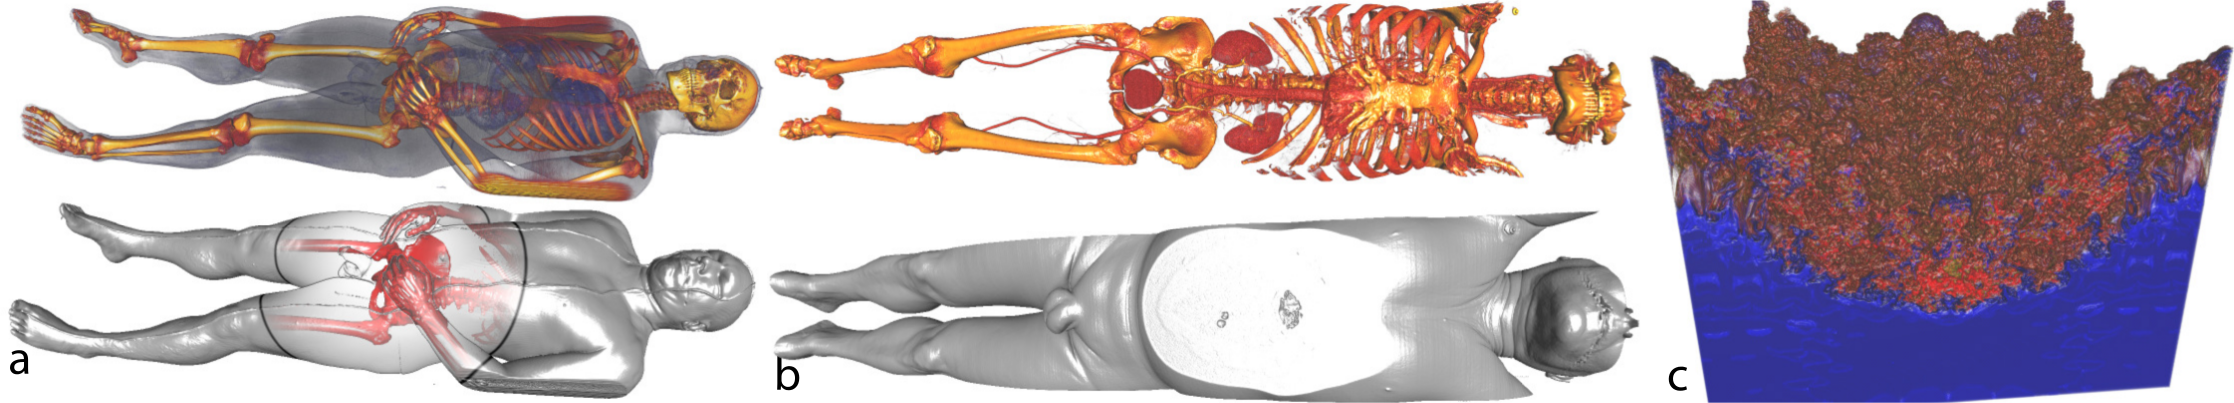
\includegraphics[width=\linewidth]{images/arch/vh-rm}

  \caption{Large data sets rendered with the \textit{Tuvok} framework.
  The Visible Human~\cite{Yoo:2000:VHuman} CT scan (a), the Wholebody
  data set (b) and a Richtmyer-Meshkov instability (c).}
	\label{figtvk:teaser}
\end{figure*}

In the past decade texture-based volume rendering on graphics hardware
has positioned itself as a powerful tool for interactive visual
analysis of modestly sized data sets. In earlier years slice-based
approaches~\cite{Cullip:1993:AVRW, Cabral:1994:AVRA} were utilized
due to the limited capabilities of older graphics hardware, with the
drawback of distracting visual artifacts. Later, GPU-based ray casting
became possible on consumer GPUs, producing superior image quality
and allowing for the integration of various acceleration
strategies~\cite{Krueger:2003:ATGV}.  In addition to improvements in
volume traversal methods, various approaches have been presented to
efficiently render data larger than the video or even the system's main
memory.

As data sizes grow, however, an efficient rendering system only solves
part of the visualization problem. Along a different line of research,
novel methods have been proposed to effectively interrogate, search,
highlight and present data with an increasing number of high resolution
features. In the course of this research multi
dimensional-~\cite{Kniss:2005:Multidim}
spatialized-~\cite{Roettger:2005:Spatialized},
size-based-~\cite{Correa:2008:Size-based}, motion
controlled-~\cite{Correa:2005:Motion},
topology-based~\cite{Weber:2007:Topology},
and style transfer functions~\cite{Bruckner:2007:Style}, as well as
other focus and context enhancing
techniques~\cite{Viola:2005:Illustrative, Wang:2005:Lens,
Krueger:2006:ClearView} have been developed. For a complete and
detailed survey on volume rendering we refer the reader to the state of
the art report, course, and books by Engel et
al.~\cite{Engel:2002:IHQV, Engel:2004:RTVG, Engel:2006:RTVG}.

Due to this vast body of research a large variety of different volume
rendering systems and prototypes exist both in academia as well as
in industry. Yet researchers and developers often reimplement the
same basic fundamentals for each new volume rendering application. It
may seem that there are many different good reasons for not reusing
existing, proven code, but one can usually categorize the decision into
one of three cases:

\begin{itemize}

  \item \textbf{System}:
	Often, the integration of new ideas and methods
	into large monolithic rendering systems proves to be a
	bigger issue than re-implementing the entire environment
	from scratch.

  \item \textbf{Software Environment}: The existing code may be
  implemented in the wrong environment, such as for an old operating
  system or graphics API. For instance, a DirectX implementation will
  not be suitable for a cross platform project. Further, many research
  prototypes are tailor-made for one system due to the lack of time and
  need for a more general implementation.

  \item \textbf{Licensing}: while largely irrelevant in the academic
  environment, license issues often prevent developers in commercial
  environments from reusing existing code. Even code that is released
  under Open Source conditions may come with untenable requirements for
  some commercial entities, such as the GPL's stipulation that related
  yet non-derivative code be released under the GNU license.

\end{itemize}

Research groups and companies often release their work and thus a
number of systems for volume rendering structured data exist as free
or open source programs. One of the earliest examples of such an
open source volume rendering system is Stanford's VolPack
software~\cite{VolPack}.  Unfortunately it has not been under
development for two decades. A more recent example is the Simian system
developed
by Kniss \textit{et al}~\cite{Simian}. Released under a very liberal
open source license, it features both a very polished user interface as
well as multi-dimensional transfer function support. Unfortunately it
falls short as far as data import is concerned and development ceased
years ago; therefore no novel render modes are implemented. Other such
discontinued frameworks and toolkits are the OGLE~\cite{OGLE} system,
optimized for large data, and OpenQVis~\cite{OpenQVis}, optimized for fast GPU
rendering. A program tailored for 3D Microscopy,
Voxx~\cite{Indiana:2009:Voxx}, has been released by Indiana University;
while it has very promising features, including support for 4D data,
it is only published in binary form.  While Bruckner and Gr\"oller's
`volumeshop'~\cite{Bruckner:2005:VolumeShop} implements unique GPU
accelerated illustrative render options, its development ceased in 2005
and no current version is available. Further, it only supported their
proprietary volume format and the current license disallows the use of
the code in commercial environments.

For medical applications the MITK toolkit~\cite{Tian:2008:MITK}
delivers many interesting features, including support for large data
sets and data manipulation routines, but it offers only basic transfer
function support and slow performance compared to highly optimized
out-of-core GPU volume rendering systems. Solely on the Apple Mac
OS X platform, OsiriX~\cite{OsiriX} offers unmatched DICOM support in
an open source application, but as the tool is tied closely to Apple's
Cocoa framework and implemented in Apple-extended Objective-C, it is
nigh-impossible to port to any other platform.

Instead of using a specialized volume rendering application,
existing visualization toolkits can be utilized to render
volumetric data. The most prominent examples are the
VTK~\cite{Schroeder:2006:VTK} and ITK~\cite{Yoo:2002:ITK} systems,
which allow for extremely versatile and flexible rendering and
modification of many types of data sets. The major drawback is the lack
of support for out-of-core processing, forcing application developers
to concoct external strategies to handle
large data sets. Built on top of VTK,
ParaView~\cite{Ahrens:2005:ParaView} addresses the large dataset
issue with a distributed memory approach but---like the underlying
toolkit---does not efficiently utilize the capabilities of modern
graphics cards, resulting in interactive performance only at very low
quality even for modestly sized data sets. Recently, the VisCG at the
Universit\"at M\"unster developed the Voreen
system~\cite{Voreen:2009}, a prototyping environment for volume
visualization.  The interface provided exposes the underlying data
flow network and many visualizations require knowledge as to how they
are technically realized, which we found was not suitable for a large
segment of our user base. Other non commercial visualization toolkits
are the OpenDX system that is no longer under active development, and
finally the SCIRun~\cite{Macleod:2004:SCIRun} and
VisIt~\cite{Childs:2005:Contracts, Childs:2012:VisIt} systems. As these
systems suffered some of the problems of previously mentioned solutions
(e.g. outdated render modes, slow performance, or limited support
for large data sets) Tuvok is currently being integrated into these
solutions. Besides these free \& open source solutions, a number of
commercial products exist such as AVS2, Amira, Ensight, syngo, VGStudio
Max, or AltaViewer. As these systems are closed source, obtaining
detailed information on their operation is difficult; the possibility
of integrating Tuvok into these systems is intriguing, but we do not
discuss them in detail for this work.

In order to address the aforementioned three issues and to overcome the
limitations of existing systems, we present \textit{Tuvok}, a system
built of cleanly separated components that can
be used together, such as in the \textit{ImageVis3D} application,
or stand-alone. The entire system is implemented in C++ with OpenGL
graphics and is designed to be completely platform independent. When
necessary, Tuvok's components can be compiled into a shared library
and accessed from another programming language. Tuvok is also released
with a modest open source license that allows unrestricted academic and
commercial use of the code. Specifically,
\textit{Tuvok} offers the following benefits:

\begin{enumerate}

\item \textbf{Large Data Support}
Given sufficient storage space, the system can theoretically
handle data sets of up to 16 Exabytes in size.
\item \textbf{Modular Design}
While the application ImageVis3D presents itself to the
end-user as a single application, it is composed of a
collection of independent Tuvok frameworks.
\item \textbf{Self contained}
While ImageVis3D requires Nokia's Qt library
as an external dependency, \textit{Tuvok} itself does not rely on
external libraries at all.
\item \textbf{Cross platform support}
\textit{Tuvok} as well as \textit{ImageVis3D} support all major platforms,
including various versions of Microsoft Windows, Apple
Mac OS X, and many Linux variants.
\item \textbf{Legacy hardware support}
Tuvok has been extensively tested to work even with the
very limited GPU capabilities of older or less capable
systems.
\item \textbf{Up To Date Rendering algorithms}
Besides its support for 2D and 3D texture based slice
based volume rendering---mostly for older graphics
hardware---\textit{Tuvok} features GPU based ray casting to
interactively render images of the highest quality.
\item \textbf{Provenance Support}
\textit{Tuvok} and \textit{ImageVis3D} provide provenance hooks, with
provenance recording and playback realized via
VisTrails~\cite{Bavoil:2005:VisTrails}.
\item \textbf{Open Source}
Tuvok and ImageVis3D are released under the very liberal
MIT license, which means that practically no usage
restrictions exist---including the use of ImageVis3D or its
components in commercial applications.

\end{enumerate}

The remainder of this chapter is organized as follows. In
Section~\ref{sec:tvk-design} we discuss the design of \textit{Tuvok},
focusing on the ways in which the library handles large data. To
demonstrate
the versatility of \textit{Tuvok} and \textit{ImageVis3D}, we describe
extensions
to the system in Section~\ref{sec:tvk-extensions}, and projects that
have
incorporated \textit{Tuvok} in Section~\ref{sec:tvk-uses}. We conclude
with a summary of the presented system and future research directions.

\section{Design}
\label{sec:tvk-design}

The ImageVis3D system is composed of three major
components, the Tuvok Volume rendering library, the Tuvok IO
library, and the Qt based UI toolkit. Note that these
components are designed to work well together but can also be
used separately or replaced by other external libraries (see
Section~\ref{sec:tvk-uses} for examples). In fact, during the
compilation process of Tuvok the subcomponents are compiled as separate
libraries that are simply linked together. During the design of these
components care has been taken to create flexible and simple interfaces
between the subcomponents. As an example of this decoupled design,
the communication from the UI to the rendering and IO systems happens
through a single entity, named the \texttt{MasterController}. This concept makes
it easy to intercept all the communication to and from the
UI (see Section~\ref{sec:tvk-extensions}) and is also the heart of the
scripting interface built into ImageVis3D, which allows programmatic
control over the application.

\subsection{The volume rendering library}

The Tuvok volume rendering library contains the core graphics
algorithms to render volumetric data. Currently, a slice based volume
renderer as well as GPU based ray casting renderer are available via
OpenGL. For pure software based rendering the system currently relies
on the Mesa library.

\subsection{Interactivity and quality}

One of the primary design goals of Tuvok is that it should be able
to visualize data sets of incredible size on almost any commodity
system. We have previously scaled the renderer to
data sizes greater than 2 terabytes~\cite{Fogal:2010:HPG}, including
the 5
terabyte rabbit eye from Figure~\ref{fig:rabbit5tb}.

This is achieved using a streaming, progressive rendering
system guaranteeing interactive frame rates with adaptive
quality. The generation of full quality imagery is also
guaranteed on all configurations, with any data set, but may not
happen interactively.

To achieve this goal Tuvok utilizes a multiresolution level of detail
(LoD) data representation. It queries the volume parameters from the
Tuvok IO Library---or an external IO framework through a documented
API if the IO library is not used---and uses that information together
with the current viewing parameters and system performance history to
compute a work order for the current render task. More
details are available in Section~\ref{sec:tvk-data}.

To achieve goals 4-6 in the list above, renderers contain a variety of
extra code paths for compatibility settings, as a means to address a
number of issues discovered in OpenGL drivers. Tuvok contains multiple
renderers, based on ray casting, 3D slicing, and 2D slicing, which span
a large range of quality versus portability across GPUs and drivers.
This has been important to support a breadth of collaborations, as
less technical users tend to have integrated graphics chips that
lack support for even 3D textures. One feature driven by this
requirement is the ability to select the bit width of the framebuffer
object (FBO) used for rendering, because we found that some drivers
would switch to a software path when rendering into a 32-bit FBO.

Table 1 gives timings for multiple data sets on different
systems, demonstrating the system's compatibility and scalability.
For these timings the progressive rendering has been
disabled: only the time to render the maximum quality
image for the given view was measured. With the progressive
rendering turned on all data sets render at the chosen refresh
rates on all systems. Note that the systems used in the test
cover chipset integrated GPUs as well as also high end PC
configurations. Timings are presented for small data sets as
well as reasonably sized CT scans and simulations. Using
even larger data sets does not significantly impact the
performance of the system, as the amount of data accessed is
bounded by the screen resolution.

\begin{table}
	\begin{tabular}{l|c|c|c}
	data set & Air & Pro & Vista \\\hline

	\begin{minipage}{0.4\linewidth}
	\textbf{C60 Molecule}\\128x128x128 8bit = 2 MB\\See	Figure~\ref{figtvk:modes}
	\end{minipage}
	& 110 / 184 & 80 / 124 & 12 / 14\\\hline

	\begin{minipage}{0.4\linewidth}
	\textbf{VH Male CT}\\512x512x1884 8bit = 471 MB\\See
	Figure~\ref{figtvk:teaser}a
	\end{minipage} & 380 / 500 & 526 / 744 & 48 / 76\\\hline

	\begin{minipage}{0.4\linewidth}
	\textbf{Wholebody}\\512x512x3172 16bit = 1586 MB\\See
	Figure~\ref{figtvk:teaser}b
	\end{minipage} & 680 / 700 & 587 / 984 & 126 / 301\\\hline

	\begin{minipage}{0.4\linewidth}
	\textbf{RM Instability}\\2048x2048x1920 8bit = 7680 MB\\See
	Figure~\ref{figtvk:teaser}c
	\end{minipage} & 5523 / 6112 & 3112 / 3520 & 196 / 321 \\

	\end{tabular}

  \caption{Tuvok timings in \textbf{milliseconds} for various data sets
  and configurations.  ``Air'': MacBook Air, 2GB RAM, onboard GeForce
  9400, ``Pro'': MacBook Pro, 4GB RAM, GeForce 9600, ``Vista'': PC
  running windows Vista, 24 GB RAM, Quadro 5800.  All tests were
  performed in isosurface mode (first value) and in 1D transfer
  function mode (second value), using the ray casting renderer and
  sampling twice per voxel into a 1024x1024 viewport.  The camera was
  zoomed such that the data set covered the entire viewport, and the
  datasets were divided into bricks of size $256^3$.}

\end{table}

\begin{figure*}
	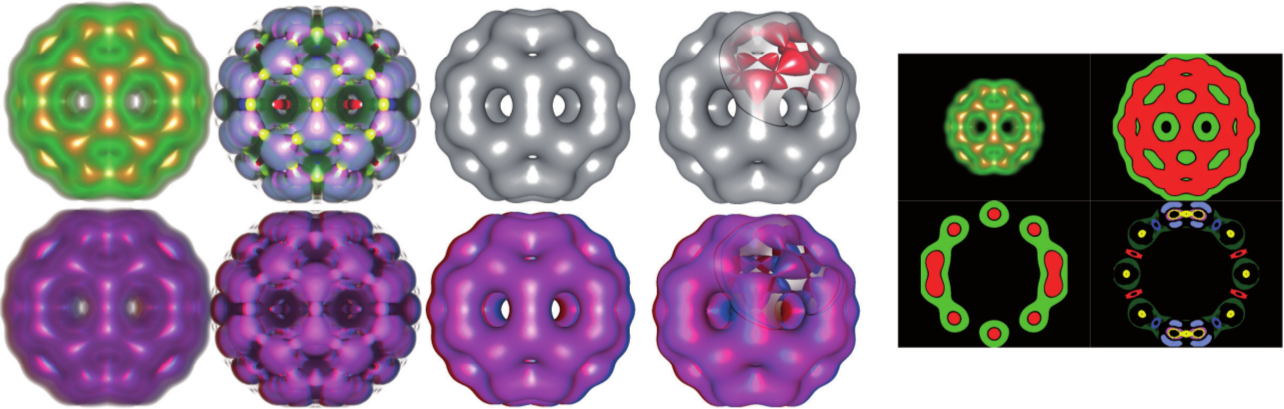
\includegraphics[width=\linewidth]{images/arch/c60modes}

  \caption{Various render modes applied to the C60 dataset.  In the
  top row 1D and 2D transfer functions, isosurface extraction, and
  ClearView are shown.  The bottom row shows the same views in anaglyph
  stereo mode.  On the right is two by two mode featuring a 3D view, a
  MIP view (top right) and two slice views (bottom).}
	\label{figtvk:modes}

\end{figure*}

\subsection{Large scale data handling}
\label{sec:tvk-data}

While Tuvok can take advantage of recent advances in hardware
capabilities, it is still true that data are growing and have been
growing faster than hardware capabilities allow. Thus, while the size
of data sets that we can interactively render is increasing with each
hardware revision, we still find that a larger percentage of our data
sets cannot be rendered interactively.  It would be unreasonable to
assume this trend would reverse in the coming years. Therefore, it is
critical that interactive visualization systems incorporate progressive
renderers.

Tuvok's progressive renderer is based on overloaded
concepts of frames and subframes. In the context of Tuvok, a
frame is a single, complete rendering of the data at native
screen and data resolution. A subframe is an intermediate
state between no rendering and a frame, which includes the
full spatial range of the data and any annotations present in
the visualization. The quality of successive subframes
monotonically increases. A sequence of these subframes are
rendered before the final frame is displayed, detailing different
approximations of the complete rendering much more
quickly than a frame can be displayed. We guarantee that
there is always at least one subframe which can be displayed
interactively (within a couple hundred milliseconds). The
system turns to such a subframe when the user is actively
interacting with the data.

To model the concepts of frames and subframes, Tuvok
uses a multiresolution, level of detail representation of data.
For the most part, a subframe corresponds to the data at
a particular level of detail. At the coarsest level of detail,
the data are small enough that they can easily be read from
disk under our real time requirements. However, we found
that older GPUs could not always render such data quickly
enough for our needs. Therefore Tuvok always makes available
up to three additional subframes. These are generated
by lowering the screen resolution of the rendering (and upscaling
before display to the user), lowering the sampling
rate used by the renderer, or both. Lowering resolution and
sample rate significantly reduces the strain on the fragment
processing stage of the graphics pipeline, allowing Tuvok
to respond quickly even on low end hardware. We do not
know any OpenGL 2.0-capable GPU which Tuvok does not
perform acceptably on, and (through extensions) Tuvok can
render even on some cards that do not report OpenGL 2.0
capabilities.

\subsubsection{Preprocessing}

Most data are not fed to visualization software with multiple
levels of detail included. To accommodate such data, Tuvok's IO
subsystem implements a preprocess which generates a multiresolution
hierarchy. The data at their native resolution form the finest level
of detail, and we subsample by two recursively until a level of detail
exists which is less than or equal to a predefined user-configured
limit. We also use this opportunity to perform other operations on
the data, such as ensuring a consistent endianness.  In most cases
preprocessed data can be loaded from disk directly into GPU memory.

The primary issues we face when loading large data are
32-bit address spaces, limitations on GPU 3D texture sizes,
and managing the IO in an efficient manner. The address
space limits us to only handling two gigabytes of data at any
one time. Limitations on texture sizes prevent us from `simply'
loading the data into a single, large 3D texture. Typical
IO performance on desktop-class and predicted future hardware
informs our strategy for how we access and consume
data.

To tackle these issues, the preprocess divides each level of
detail into a set of bricks, with each brick small enough to fit
into the texture memory of any modern GPU. The rendering
core will render each level of detail in an out-of-core fashion:
a brick will be loaded, rendered, and discarded as a single
atomic operation. This allows the renderer to load data of
virtually unlimited size with very little available memory, as
the required amount of memory is independent of the data
set size. To achieve the IO performance we require, the IO
library uses large reads (by default, 16 megabytes) that make
seek times virtually irrelevant.

A simple survey of modern disk drives finds reported seek
times ranging from 3.75 up to 8.9 milliseconds. Sustained
transfer rate capabilities can be as low as 65 MB/s; see
Table~\ref{tbl:disks}.  While there are of course differences across
drives and manufacturers, multi-megabyte reads very quickly overtake
seek times as the predominant factor in disk transfers. At 65 MB/s,
it takes almost a quarter of a second to read 16 megabytes of data,
yet only 8 milliseconds to seek to the position of that block. Even as
one gets into the higher end drives, the story is the same; a Cheetah
15K.5 would take 0.12 seconds to read a 16 megabyte chunk of data, and
only 3.75 milliseconds to seek to the appropriate location on disk.
In relative terms, seek time makes up approximately 3\% of the time
required to read the data block. Based on these simple calculations, it
is clear that transfer rates will have to improve drastically before
seek times become a relevant parameter.

\begin{table}
	\begin{center}
	\begin{tabular}{l|cc}
	\textbf{Drive name} & \textbf{Seek time (ms)} &
		\textbf{Sustained transfer rate (MB/s)}\\\hline
	Cheetah 15K.5 SAS & 3.75 & 73 to 125\\
	WD Caviar RE2-GP & 8.9 & 84\\
	Barracuda 7200.8 & 8 & 65\\
	WD 740GD & 5.2 & 72\\
	\end{tabular}
	\end{center}

	% note to self: you already updated the year, here, for your dissertation!
  \caption{Relevant disk performance characteristics for disks ranging
  from high-end server drives (Cheetah 15K.5) to an aging model
  released 11 years ago (WD 740 GD)}
	\label{tbl:disks}
\end{table}

We have also benchmarked our I/O subsystem using solid
state drives. Table~\ref{tbl:ssd} shows the time spent on I/O when
loading a 648-brick data set via Tuvok. The SSD boasts vastly better
seek times, on the order of microseconds instead of the normal
milliseconds for mechanical drives, and a factor of two to three
improvement in bandwidth. Using large reads, the seek time matters
little in this case, but as shown in Table~\ref{tbl:ssd} Tuvok benefits
from the improved transfer times offered by SSDs.

\begin{table}
	\begin{center}
	\begin{tabular}{|c|c|}\hline
	\textbf{3-disk SATA RAID5} & \textbf{Solid state drive}\\\hline
	64.8704 & 27.6723\\\hline
	\end{tabular}
	\end{center}

  \caption{I/O component (seconds) for rendering a 9 gigabyte timestep
  from a simulation of a Richtmyer-Meshkov instability.}
	\label{tbl:ssd}
\end{table}

\subsubsection{Paging strategy}

Transfer time forms the majority of our pipeline execution time when
using high end GPUs. Therefore, by maintaining a cache for individual
bricks, we can improve the overall rendering time by obviating the
transfer time for oft-requested bricks.

A straightforward paging strategy for such a cache would
be Least Recently Used (LRU), however this strategy delivers
poor performance in many situations. Consider a dataset
with 10 bricks, and a brick cache capable of storing 9 bricks.
In the first frame, all ten bricks must be paged. Further, loading
the final brick of the first frame will evict the first brick
of that frame. Assuming any reasonable amount of frame-to-frame
coherence, the next frame will again need the same 10
bricks, and they are likely to require a similar depth ordering.
Thus, in the second frame, the first brick we will need
is the brick we just evicted at the end of the last frame; further,
the second brick we need will be evicted while loading
the first brick of the second frame, and so on throughout the
entire frame.

We have implemented a custom paging strategy that
takes into account our progressive rendering system. In this
strategy, we evict bricks \emph{within} a frame using the Most Recently
Used (MRU) strategy; we evict bricks \emph{between} frames using the
LRU strategy. The rationale for the former is that once we have used a
brick in a subframe, it will not be used in the rendering of that frame
again until the progressive renderer starts over, and we may service
a large number of bricks in the interim. However, if we do start the
frame from its earliest subframe again, particularly before finishing
the frame, we are likely to need the oldest bricks which are present
in the cache. Between frames, we rely on frame-to-frame coherence. If
a brick was not used in the previous frame, and is not used in the
current frame, it is likely to not be required in subsequent frames as
well; a common example is if the user has enabled a clip plane: any
viewing transform will not affect the bricks that are clipped away by
the plane. Therefore the LRU strategy will tend to evict bricks that
are not visible under the current transfer function, isosurface, or
viewing parameters.

\subsection{UI and networking library}

To facilitate rapid development of other visualization applications,
all those components built on top of Qt which are
not specific to the application level were separated, allowing
them to be shared and reused in future applications. These
components can be roughly categorized as the UI and networking
components. The independent networking components
include the bug reporting, update checking, and data
set sharing subsystems, while the UI components include
the base classes that define the look and feel of ImageVis3D,
such as dialogs, tool widgets, user interaction, and persistence.

\section{Extensions to \textit{Tuvok} and \textit{ImageVis3D}}
\label{sec:tvk-extensions}

In this section we present a couple of examples to
demonstrate how simple it is to add new features or extend
existing functionality. We present examples from research
projects implementing a prototypic environment to experiment
with new methods (\tjfsec{sec:arch-rendering-exts}) as well as new
features to ImageVis3D to use it for other research.

Due to the modular design, the scripting interface, and
the \texttt{MasterController} concept, integration with external
software is simple. As the UI and execution layer communicate
strictly through a single class, the \texttt{MasterController}, any
type of external communication channel can simply attach
itself to this class and track changes. Control of the library
can also happen through the \texttt{MasterController} via script
commands that allow programmatic modification of all of
Tuvok's features.

\subsection{Extensions to the rendering subsystem}
\label{sec:arch-rendering-exts}

ImageVis3D has been extended to provide domain specific
visualization capabilities. In some domains, it is necessary
to visualize multiple data sets simultaneously. A student has
modified ImageVis3D to render multiple data sets that live in
overlapping space, and added domain-specific widgets for
ease of use in a particular scientific domain. One such example
is a dialog to automatically create transfer functions,
based on external knowledge of characteristic data distributions
within data sets common to that field. A second example
is repurposing the 2D transfer function editor to utilize
different metadata along each axis.

\subsection{Extensions to \textit{Tuvok}'s controller}

For provenance tracking, we have integrated VisTrails, a production
provenance framework with well-developed APIs
for integration with external systems. The integration of
VisTrail’s provenance tracking features required a two way
communication from and to Tuvok. Interactions made by
the user need to be communicated to VisTrails to track the
provenance, but also VisTrails needs to be able to control Tuvok
to perform undo/redo operations. Thus, this example is
prototypic for any type of recording or remote control of Tuvok,
such as cluster extensions or connections to novel input
devices.

\section{Use cases of \textit{Tuvok}}
\label{sec:tvk-uses}

\begin{figure*}
	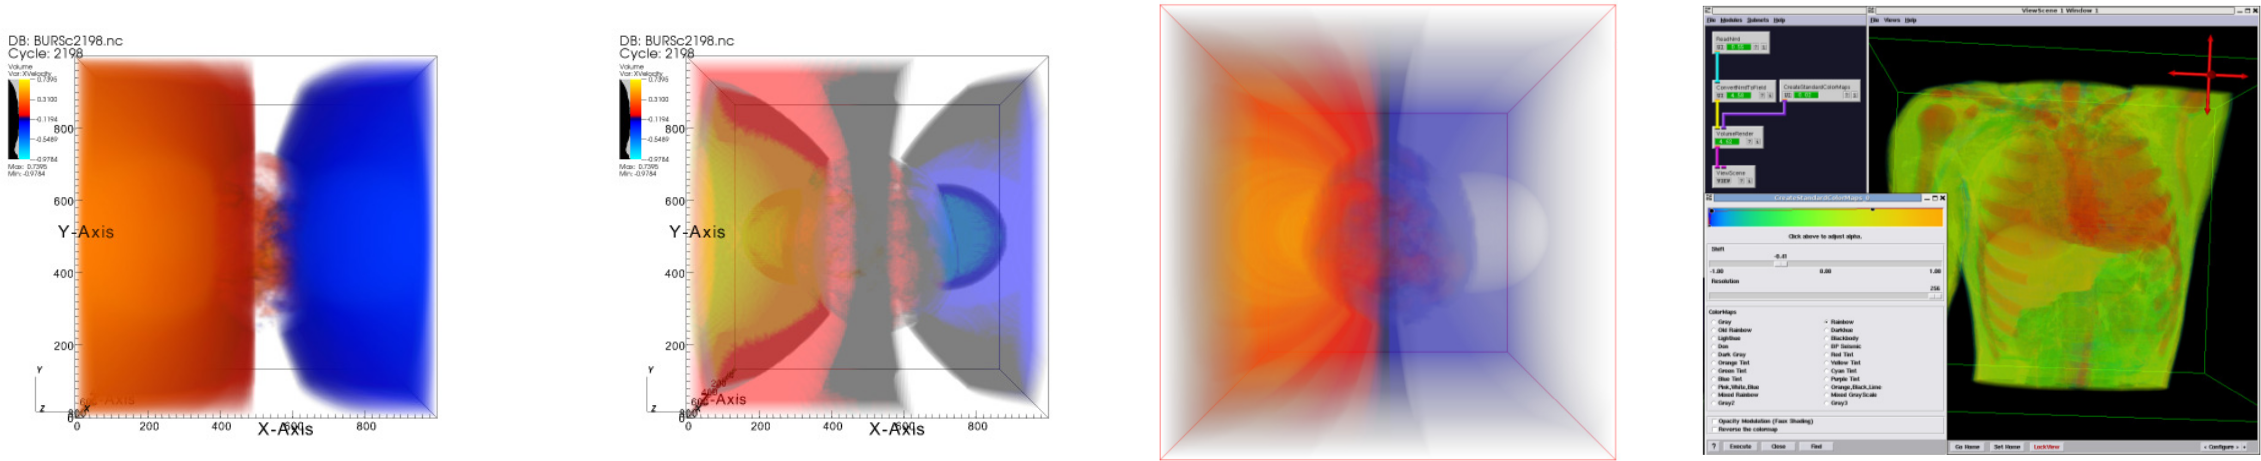
\includegraphics[width=\linewidth]{images/arch/integration}

  \caption{3D texture, SLIVR, and \textit{Tuvok} volume renderers in
  VisIt (left); \textit{Tuvok} rendering a torso in SCIRun (right).}
	\label{figtvk:integration}
\end{figure*}

In the following we present examples where Tuvok---or only some of it
components---have been integrated into rendering environments other
than
\textit{ImageVis3D}. Figures~\ref{figtvk:integration}
and~\ref{figtvk:altaviewer} demonstrate the integrations presented here.

\subsection{SCIRun}

SCIRun is a problem solving environment for modeling,
simulation, and visualization of scientific data. It is an example
of what we refer to as a legacy application, in that it
was developed without the ideas implemented by Tuvok in
mind. In particular, this means that the system must work
with in-core, `unbricked' data sets of a single resolution.

To support such an environment, Tuvok has a simplified
API for existing systems which do not include level of detail
or bricking concepts. The information flows one way from
the controlling application to Tuvok, and includes a reference
counted smart pointer to the data, as well as metadata
and rendering parameters. For small changes in rendering
parameters, data shared from previous frames is retained and
simply re-rendered. When changing or passing a new data
set to Tuvok, the old data set is removed and replaced by
a new reference counted smart pointer. This scheme allows
us to avoid data copying between the host application and
rendering library. In these kinds of systems, Tuvok does not
have access to a multiresolution form of the data, and thus
cannot guarantee interactive performance.

\subsection{VisIt}

VisIt is a data visualization and analysis application which is
well-suited to large scale data processing on leadership computing
platforms. We have integrated the underlying rendering
core as an option alongside VisIt's existing volume renderers.
Since VisIt already supported domain-based data set
decomposition, it can easily take advantage of an additional
Tuvok feature: bricking. This allows VisIt to volume render
data of arbitrary size on the GPU, whereas it was previously
limited to resampling the data or utilizing software rendering.

Though data do not come directly from a data file in this
and other integration work, the abstraction provided by Tuvok's
IO layer allows the rendering core to remain ignorant
about the source of the data. The metadata which must be
supplied to Tuvok scales with the complexity of the application:
in the unbricked, SCIRun case, Tuvok can be told only
the brick size (assuming the brick lies centered on the origin);
with decomposed data, Tuvok must be informed of the
world space location of the bricks; for progressive rendering
applications, such as ImageVis3D, the LoD that a brick belongs
to must also be given. Should an application choose, it
can also supply additional metadata to allow advanced rendering
optimizations.

An issue that arose specifically in the VisIt integration
was state management in large, established software systems.
The OpenGL API is a global state machine, and VisIt
has many sub-libraries which can and will change the global
state in ways we cannot predict. Tuvok therefore makes very
few assumptions about OpenGL state. During the `setup'
stage, Tuvok takes state information---camera and viewing
reference points, data, etc.---and stores it locally.
A single method then uses all that information to configure
OpenGL state once before moving on to per-brick rendering.
For efficiency reasons, the system leaves the OpenGL
state `as-is' when finished rendering, much like other VisIt
subsystems and libraries do. Until OpenGL establishes an
object model, we have found this to be the best method for
managing OpenGL state.

\subsection{AltaViewer}

\begin{figure}
	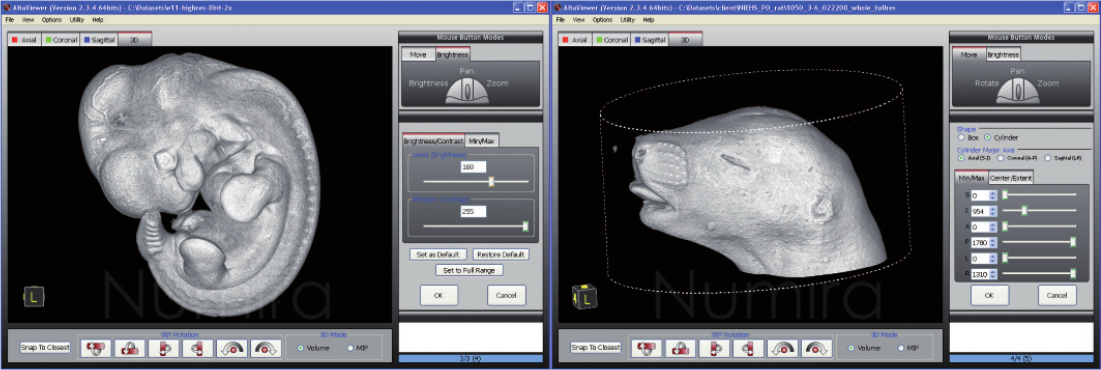
\includegraphics[width=\linewidth]{images/arch/altaviewer}

	\caption{The left image shows an E11 mouse embryo
	(2.4GB) while the right image depicts a P0 newborn rat
	(7.6GB). Both specimens were stained using Numira's custom
	protocol and scanned using microCT. Images courtesy
	of Numira Biosciences. Copyright 2009 \copyright{} Numira Biosciences.
	All rights reserved. AltaViewer Software available
	at \url{http://www.numirabio.com/}}
	\label{figtvk:altaviewer}
\end{figure}

Finally, we demonstrate the usability of Tuvok's components
in a commercial environment. Numira Biosciences is a specialty
contract research organization (CRO) which focuses
on high-resolution imaging and analysis of small animal
specimens, provides researchers with quantifiable, visible
evidence of disease progression, as well as drug efficacy and
drug side effects in their animal models. For the next generation
of their visualization suite `AltaViewer' (see
Figure~\ref{figtvk:altaviewer}) they have chosen to replace their
proprietary IO library in part by Tuvok's IO components to achieve
significantly better performance.

\section{Conclusion and future work}

In this paper we have presented the Tuvok framework as well
as ImageVis3D, an application built with Tuvok. We gave insight
into large data support in a production volume renderer.
We also gave a couple of examples of research projects and
commercial use of components of Tuvok.
We are currently working on three major extensions to
Tuvok. First, the support of time dependent data sets, in
particular we are working to extend the progressive rendering
concept to this data as well. Secondly, we are extending
Tuvok to render multiple data sets in overlapping 3D space;
due to the out-of-core nature of the system an efficient
implementation of this feature is non-trivial. Finally, we also
plan to add purely software based as well as OpenCL based
ray casters to allow for fast rendering of ultra large data sets
on headless clusters with and without GPUs.


\chapter{Ray-guided volume rendering}
\label{chp:rayguided}
\begin{figure*}
  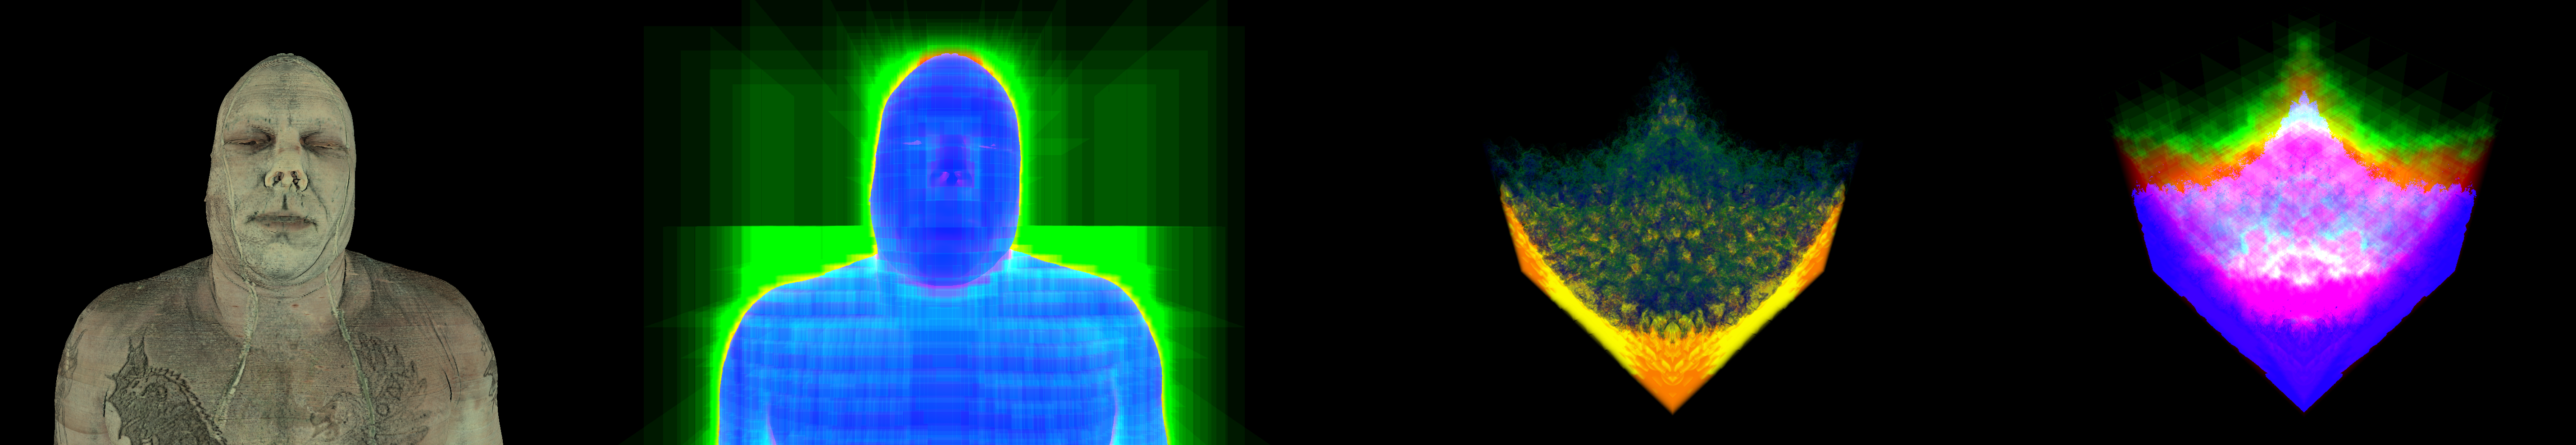
\includegraphics[draft=\isDraft, width=1.00\linewidth]{images/rg/teaser.png}
  \caption{The Visible Human male full color (\tjftilde{}12~GB) and
  a Richtmyer-Meshkov instability (\tjftilde{}8~GB) render in 34~ms
  and 58~ms, respectively, using our ray-guided volume rendering
  implementation.  On right are views that highlight the areas
  that take advantage of empty space leaping (green) and early ray
  termination (blue).}
  \label{figrg:teaser}
\end{figure*}

Volume rendering continues to be a critical method for analyzing
large-scale scalar fields, in disciplines as diverse as biomedical
engineering and computational fluid dynamics.
% On the one side,
% ever-increasing scanner capabilities has resulted in the proliferation
% of datasets with vastly increased resolution.  On the other, massive
% parallel supercomputing resources has enabled simulations at
% unprecedented resolutions.
Commodity desktop hardware has struggled to keep pace with data
size increases, challenging modern visualization software to
deliver responsive interactions for $O(N^3)$ algorithms such as
volume rendering.  We target the data type common in these domains:
regularly-structured data.

In this work, we demonstrate that the major limitation of most volume
rendering approaches is their inability to switch the data sampling
rate (and thus data size) quickly.  Using a volume renderer inspired by
recent work, we demonstrate that the actual amount of visualizable data
for a
scene is typically bound \emph{considerably} lower than the memory
available on a commodity GPU.  Our instrumented renderer is used to
investigate design decisions typically swept under the rug in volume
rendering literature.  The renderer is freely available, with binaries
for all major platforms as well as full source code, to encourage
reproduction and comparison with future research.

\section{Introduction}

Modern volume rendering is heavily focused on the concepts of empty
space skipping and the fast detection of ray saturation.  Both of
these concepts have extensive effects on the amount of compute work
required.  However, even more relevant is their ability to reduce the
working set of extremely large datasets down to a small kernel, which
can significantly reduce the amount of data that must be loaded from a
slow resource, such as the network or a local disk.  This has enabled
interactive volume rendering for very large data on commodity
hardware~\cite{Knoll:2010:BVH, Hadwiger:2012:Guided,
Crassin:2009:Gigavoxels}.

There are a variety of trade-offs in the development of a modern volume
renderer.  The choice of brick size, for example, can significantly
impact the effectiveness of empty space skipping.  We note that the
presentation of most volume rendering systems lacks detailed insight
into these parameters.  Further, these factors can interact in complex
ways.  As an example, empty space skipping works considerably better
with smaller bricks sizes, but disk throughput drops sharply with small
requests.  Compression can further complicate the issue.

We seek to rectify this situation by performing a thorough study of
the interaction of these parameters within the context of GPU-based
ray driven volume rendering.  We have surveyed recent volume rendering
literature and implemented a renderer by piecing together the best
ideas from a multitude of systems. These ideas were extended with
notions required for our environment---for example, by removing
the requirement that datasets fit in GPU memory.  Along the way,
we instrumented every corner of the renderer and utilized this
instrumentation to exhaustively explore relevant options.  The final
result achieves better performance than previous work and provides a
guided tour through the maze of design choices available in a modern
volume renderer.

\begin{figure*}
  \centering
  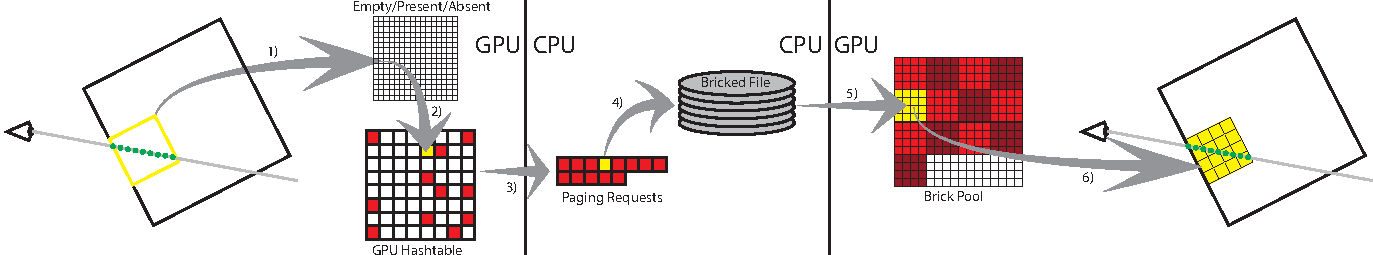
\includegraphics[width=1.00\linewidth]{images/rg/pipeline.pdf}
  \caption{The missing brick reporting / paging subsystem of our volume
  rendering approach.  Missing bricks are recorded into a hash table
  (1, 2), to be paged in (3, 4, 5) and rendered in subsequent frames
  (6).}
  \label{figrg:flow}
\end{figure*}

\section{Related Work}

Volume visualization on consumer graphics hardware has become widely
utilized as a means to cope with the growing sizes of data.  GPUs have
proven useful in both ray-tracing and rasterization
techniques~\cite{Reichl:2012:HybridSurface, Dick:2009:Terrain},
rendering of diverse scenes~\cite{Parker:2010:Optix}, as well
as considerably more general tasks~\cite{Owens:2007:GPGPU}.

Volume rendering accelerated by GPU hardware was established in the
mid-90's~\cite{Cullip:1993:AVRW, Cabral:1994:AVRA}, initially based on
hardware compositing of volume slices.  The ability to do raycasting
came later~\cite{Krueger:2003:ATGV}.  Since the time of the initial
GPU-based volume renderers, researchers have been concerned with
methods to work around the limited memory available on GPUs.  The
prominent technique for volume rendering large data on a GPU is to use
a multiresolution
representation~\cite{Boada:2001:Multires, LaMar:2000:Multires,
Weiler:2000:LoD}.  This method hinges on the concepts of empty space
leaping and early ray termination~\cite{Levoy:EarlyTermination}, two
techniques developed early on that demonstrate that sampling can be
significantly reduced in many instances of volume rendering.

There has been much work on accelerating ray-traced volume rendering in
recent years.  Voreen implements a more general architecture,
including GPU-based raycasting~\cite{Voreen:2009}.  Tuvok implements a
flexible volume rendering system with support for very large
datasets~\cite{Fogal:2010:Tuvok, Fogal:2009:SizeMatters}.  Knoll et al.
utilize a bounding volume hierarchy and optimized SSE to achieve very
fast
volume renderings~\cite{Knoll:2010:BVH}.  Gobbetti et al. and Boada et
al. detail methods for traversing tree structures on the GPU for
the purpose of volume rendering~\cite{Gobbetti:2008:VR,
Boada:2001:Octree}.
The Gigavoxels~\cite{Crassin:2009:Gigavoxels} system traverses
$N^3$-trees on the GPU to choose an effective resolution.  With the
large gap between processing power and data sizes, some communities
have turned to distributed memory systems for large-scale
volume rendering~\cite{Childs:2006:ScalableVR, Howison:2010:MPIHybrid,
Fogal:2010:HPG, Beyer:2012:DSM}.

Our algorithm employs a lock-free data structure on the GPU for
feedback information.  Highly-concurrent Lock-free structures are ideal
for the manycore GPU environment, however they have previously been
challenged by the lack of concurrency primitives available for the
OpenGL platform.  We make use of a lock-free hash table very similar to
that of Michael's~\cite{Michael:2002:LockFreeHT}, implemented in a
manner similar to Lux and Fr\"ohlich's implementation for terrain
rendering~\cite{Lux:2011:RCHeight}.

Hadwiger et al. presented a volume renderer similar to
ours~\cite{Hadwiger:2012:Guided}.  Their system is aimed at volume
rendering highly anisotropic data as it is streamed real-time from a
high-resolution microscope.  Our renderer improves upon theirs in a
number of ways:

\begin{itemize}
  \itemsep0em
  \item We perform brick lookup each brick, instead of every sample,
  maintaining the simple and familiar ray-marching core that is
  well-documented in volume rendering literature.

  \item We expound on how to use modern GPU features to implement our
  lock-free feedback data structure.  This enables the implementation
  to spend more time computing on the GPU and less time pushing data
  around.

  \item We utilize an out-of-core, progressive rendering methodology,
  breaking the GPU-memory-size barrier that limits data sizes from
  Hadwiger et al.'s work.  This also allows us to gracefully scale down
  to consumer-level graphics cards.
\end{itemize}

While we believe these to be novel additions, we do not consider them
to be this work's major contribution.  Rather, we provide new depth to
the discussions of a variety of parameters that are relevant in the
development of a ray-guided direct volume renderer:

\begin{itemize}
  \itemsep0em
  \item The strategy to be used to load higher resolution data when a
  variety of intermediate choices are possible;

  \item an understanding of the miasma of issues surrounding bricking
  and brick sizes;

  \item empirical evidence demonstrating that the working set for
  direct volume rendering is indeed bound more by the screen resolution
  than the dataset;

  \item a novel method for ray-guidance storage and propagation to the
  input system's logic;

  \item how to effectively handle real-time updates to the transfer
  function; and

  \item the effect of brick layout strategies on large volume access
  times.

\end{itemize}

% improvements upon gigavoxels:
%  . we don't require a hierarchy (but of course one can be used)
%  . they use MRTs to store their information on which brick is
%    needed.  this (a) wastes their MRTs, of which one only has 8
%    on modern GPUs, and (b) means that their memory for doing
%    this is extremely limited.  since we use image_load_store,
%    our HT for storing this is decoupled from the actual
%    rendering, and can scale up (or down) arbitrarily

In contrast to previous renderers, ray-guided volume renderers couple
the rendering process with the identification of which subvolumes
(`bricks') must be loaded.  We describe the operation of ray-guided
volume renderers, in Section~\ref{sec:algorithm}.
In Section~\ref{sec:performance} we detail a plethora of benchmarks
that demonstrate the performance of the renderer.

In many prior volume renderer evaluations, results are generally
limited to the raw performance of the renderer.  However, we note
that---for some reason---users of our volume renderer rarely ask how
many milliseconds it takes
to render the visual human.  One thing users \emph{do} ask is how large
the data can get before the renderer becomes unusable. For this reason,
we have engineered our renderer so that it does not require that the
volume fit in core.  Furthermore, users generally value a responsive
system over a performant system.  They are curious if money should be
spent upgrading a video card or buying a solid state drive.  Design
elements are carefully expounded and conclusions are drawn in
Section~\ref{sec:tradeoffs}.

Finally, Section~\ref{sec:conclusion} gives our final remarks, and note
both limitations and opportunities for future work.

\section{Ray-Guided Grid Leaping}
\label{sec:algorithm}

At the macro level, our algorithm is reminiscent of the recent work of
Hadwiger et
al.~\cite{Hadwiger:2012:Guided}, as well as Engel's
CERA-TVR~\cite{Engel:2012:CERA} that is in turn based on the Gigavoxels
system~\cite{Crassin:2009:Gigavoxels}.

With Hadwiger et al. we share the requirement of a set of simple
multiresolution Cartesian grids, along with an OpenGL-based table
to report missing bricks.  A multiresolution hierarchy is built as a
preprocess for input data that exist at only one resolution (details
are in Section~\ref{sec:tradeoffs}).  From the CERA-TVR system
we inherit the idea to only recompute and request grid cells at
boundaries.

\subsection{Overview}

We endeavor to create a volume renderer that can render massive 
datasets extremely fast on commodity GPU hardware.  The major issues in
such a renderer are:
\begin{enumerate}
  \itemsep0em
  \item Identifying regions that must be sampled densely.

  \item Precisely locating the transition between these regions and
  regions that exhibit considerable homogeneity.

  \item Terminating a ray as soon as possible.

  \item Efficiently communicating regions to be rendered in the future
  to the IO layer.

\end{enumerate}

Points (1) and (2) ensure we concentrate the computational effort on
the areas that require it.  Point (3) is critical because it means we
do not have to load the data beyond the point of early termination,
significantly reducing costly disk traffic.  If point (4) is not
sufficiently addressed, the renderer will load large amounts of data
that are not needed for rendering, at severe costs in performance.

% new subsection header here? we are switching from properties a
% Ray-guided VR needs to how we implemented said properties, here

To the first point, we employ an efficient metadata structure that
allows us to quickly identify these regions.  Points (2) and (3) are
handled through an educated choice of brick size, which is discussed
more thoroughly in Section~\ref{sec:tradeoffs}.  A major component to
modern volume renderers is how they address point (4), now by and large
based on \emph{ray guidance}.  That is, the sampling characteristics of
the ray determine which data to load.  Stated differently, the future
data requirements are computed \emph{in concert} with standard ray
traversal and accumulation.

% \todo{here we might want to say something about how regular disk I/O
% is in modern volume renderers, and allude to a later section where we
% discuss data organization}

The entire operation is detailed in Figure \ref{figrg:flow}. For each
ray we compute the level of detail required to maintain a pixel error
of less than one. With this level and the position in the volume we
compute a brick index.  This brick index is used to fetch information
from a lookup table
(Figure \ref{figrg:flow}.1) to identify whether the brick is a) empty, b)
non-empty and present on the GPU, or c) non-empty and absent. When it
is empty, we skip the brick and repeat the process at the brick's exit
point.  When it is non-empty and present, we ray-cast that brick. When
the brick is non-empty \emph{and} not resident in GPU memory, the
system returns the finest coarser level available and the missing entry
is added to a GPU hash table (Figure
\ref{figrg:flow}.2). This table is read back to the host memory at the
end of the frame (Figure \ref{figrg:flow}.3), and used to page in bricks
from
disk or cache (Figure \ref{figrg:flow}.4).  A paged-in brick is then
uploaded to a GPU texture pool
(Figure \ref{figrg:flow}.5), and a subsequent frame will use this
portion of the brick pool for sampling (Figure \ref{figrg:flow}.6).

% While we do not require a full hierarchy---only that coarser versions
% of the data exist---we generate a multiresolution hierarchy for such
% data as a preprocess.

The key component is that both ray-accumulation \emph{as well
as} identification of the bricks that are needed should occur
on the GPU.  The latter is natural to compute during standard
ray-casting operations.  Doing both operations on the GPU means brick
identification comes very cheap, as it parallelizes very effectively.
More importantly, performing this during ray-casting ensures that it
is optimally accurate: the program never loads data that will not be
used.

%---we get results which are as accurate as the brick size.

\begin{algorithm}
  \caption{Ray-guided volume rendering.  Each ray identifies the
  set of bricks that it needs for rendering independently, and
  reports this information for use in subsequent rendering passes.}
  \label{alg:vrender}
  \begin{algorithmic}[1]
%  \If{$rayResumePos = FINISHED$} \Return \EndIf
  \State \textit{color} = \textit{rayResumeColor}
  \State \textit{terminated} = \textbf{true} \Comment{assume ray will finish}
  \State \textit{rayResumePos} = \textbf{FINISHED}
  \Repeat
    \State \textit{LoD} = ComputeLOD(Depth(\textit{ray}))
    \State \textit{brick, samplingRate} = GetBrick(\textit{ray})
    \State \textit{offsets} = PoolOffsets(\textit{brick})
    \If{\textit{samplingRate} $\neq$ RequiredSamplingForLOD(\textit{LoD})}
      \State ReportMissingBrick(\textit{brick})
      \If{\textit{terminated}} \Comment{\emph{first} missing brick?}
        \State \textit{terminated} = \textbf{false}
        \State \textit{rayResumePos} = \textit{ray}
      \EndIf
    \EndIf
    \State Raycast(\textit{ray}, \textit{samplingRate}, \textit{offsets})
  \Until{\textit{ray} $\geq$ \textit{exit} $\lor$ Saturated(\textit{ray})}
  \State \textit{rayResumeColor} = \textit{color}
  \end{algorithmic}
\end{algorithm}

The basic algorithm is given in Algorithm \ref{alg:vrender}.  Briefly, the
appropriate sampling rate is identified and we look for the data at
that resolution (lines 6, 7).
\texttt{GetBrick} will always return some data, but the data may be at
a lower resolution than request; this is
communicated through the \texttt{samplingRate} and the situation is handled
on line 8.  If our data are too coarse, we note that we are missing a
brick (\texttt{ReportMissingBrick}) and where we are in the volume
(\texttt{rayResumePos}) when
this \emph{first} occurred (\texttt{terminated}).

% A key insight is that the relationship between \texttt{GetBrick} and
% multiresolution data can be entirely opaque.  The function simply
% takes a region and returns a chunk of memory to be ray-traced, with
% information as to how it should be sampled.  In contrast to the
% Gigavoxels system, a strict hierarchy is not required, and indeed our
% system does not organize data on the GPU in this manner.

% \begin{algorithm}
%   \caption{Ray-casting inner loop.  Operation is equivalent to a
%   traditional ray-casting volume renderer, with the minor addition
%   of offsets into the volume pool.  Checking in the outer loop is
%   sufficient and allows this core inner loop to stay simple.}
%   \label{alg:inner-loop}
%   \begin{algorithmic}[0]
%     \While{$ray \not\geq$ Exit($brick$)}
%       \State $v =$ sampleVol($ray$ + $offsets_{pool}$)
%       \State $c =$ TransferFunction($v$)
%       \State $color = color + (1 - \alpha) \times c$
%       \State $ray = ray + stepSize$
%     \EndWhile
%   \end{algorithmic}
% \end{algorithm}

Every iteration through the outer loop, we perform this identification
of the appropriate resolution.  This satisfies our first goal as
mentioned above: we identify the appropriate sampling resolution
at every brick boundary.  With small bricks, this means we will do
few integration steps before early ray termination is recognized.
Furthermore, we detect empty bricks at this stage as well.  The
standard
raycasting inner loop is hidden in the \texttt{Raycast} call.

% The \texttt{Raycast} function is listed in Algorithm
% \ref{alg:inner-loop}.  Note that this is equivalent to `standard'
% ray-casted volume rendering in more traditional volume renderers,
% sans the minor addition of \texttt{offsets} when sampling the
% volume data.  In fact, this is not a unique aspect of our renderer;
% any renderer which uses a volume pool would share this code.  The
% simplicity of the volume rendering loop is a prime benefit to our
% approach; the entire GLSL core consists of less than 600 lines of code,
% including all the debugging and profiling targets used to generate
% images and timing results for this paper.

% \subsection{Mixed Levels of Detail}
% 
% As the sampled resolution can differ at arbitrary points along the ray,
% a natural concern is what sampling methodology is required to ensure
% these boundaries are not visible in the rendering.  In this section, we
% demonstrate empirically that no advanced sampling schemes are required.
% 
% The appropriate sampling rate for a given region of space is a function
% of the frustum settings and the depth of the current sampling position.
% The depth is the only parameter which varies
% \emph{while} we progress along a ray.  Moreover, the appropriate
% sampling rate is aliased to the relatively few levels of detail which
% are available for a dataset.
% 
% \begin{figure}
%   \centering
%   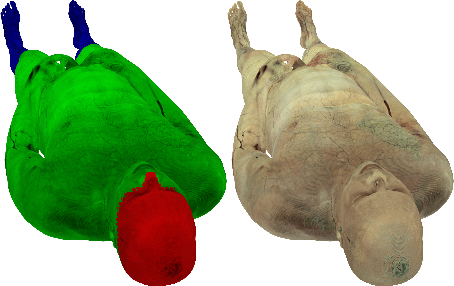
\includegraphics[width=\linewidth]{images/simultaneousLoDs-1}
%   \caption{Volume rendering of the full color visible human dataset
%   with color-coded levels of detail.  It is difficult to derive viewing
%   conditions for which a plethora of LoDs are required; the relatively
%   few LoDs visible here come from an extreme case.}
%   \label{figrg:LODs}
% \end{figure}
% 
% In practice, even for highly anisotropic data, it is difficult to
% derive frustum and viewing angles which result in the simultaneous
% visibility of more than three levels of detail.  Figure
% \ref{figrg:LODs} demonstrates this: as the ray switches from one level
% of detail to another, the color is flipped---bricks rendered at the
% highest resolution for the viewpoint are in red, and the lowest
% resolution data has a blue tint.  Looking at these areas side-by-side,
% it is clear that such boundaries are not visible in normal volume
% renderings.
 
%% this was moved to a single sentence at the beginning of sec:algorithm
% \todo{This paragraph feels really out of place here, but we need something
% similar \emph{somewhere} (reviewer comment)} Of course, many volume
% datasets are not provided in a multiresolution form.  For such data,
% we generate multiresolution representations as a preprocess.  This need
% only be done once, of course, and is relatively fast: 72 minutes on
% a modern Intel i7 machine for a typical case, the Richtmyer-Meshkov
% instability (`RMI', $2048x2048x1920$ voxels).  We note, however, that
% this process scales very poorly with the brick size: small brick sizes
% take considerably more time. More
% discussion is provided in Section~\ref{sec:tradeoffs}.

% or 5391.92 seconds / 60 = 89.87 minutes on a Xeon

\subsection{Missing Data}

As noted above, it is possible that data are undersampled while
rendering.  When this occurs, we display a coarser version of the data
initially, but progressively refine those regions with finer resolution
data until they are sampled at a rate of a single voxel per pixel, or
the maximum data resolution available.  This information is collected
by the GPU as it renders, but must be communicated back to the CPU to
coordinate disk access and update the appropriate area of the volume
pool.

One solution for this would be to use multiple render targets to store
information on which bricks are missing~\cite{Crassin:2009:Gigavoxels}.
The limitation of this method is the limited mapping operation from
the ray to the target buffer: there are only so many available render
targets.
Furthermore, this approach ignores the inherent spatial coherency
between rays.  Two neighboring rays are highly likely to request the
same set of bricks, or at least have substantial overlap within the
sets they require.  With the multiple render targets approach, both
pixels will encode the same value, and we will need to read back larger
textures that consist of predominantly duplicate values.

Instead of utilizing extra render targets, we take advantage of an
OpenGL extension that was promoted to core in version 4.2,
\texttt{GL\_ARB\_shader\_image\_load\_store}.  This extension allows
the creation of an image buffer that is independent of the current
rendering buffer.  Using the atomic load/store operations the extension
provides, we implement a set based on a linearly-probed lock-free hash
table stored in an \texttt{image\_load\_store} buffer.  Since we are
hashing based on the brick, multiple rays requesting the same brick hash
to the same position.  This allows us to keep the table---and therefore
how much information we read back per-frame---quite small.  We discuss
sizing of the hash table in more detail in
Section \ref{sec:ht-params}.

\begin{figure}[t]
  \centering
  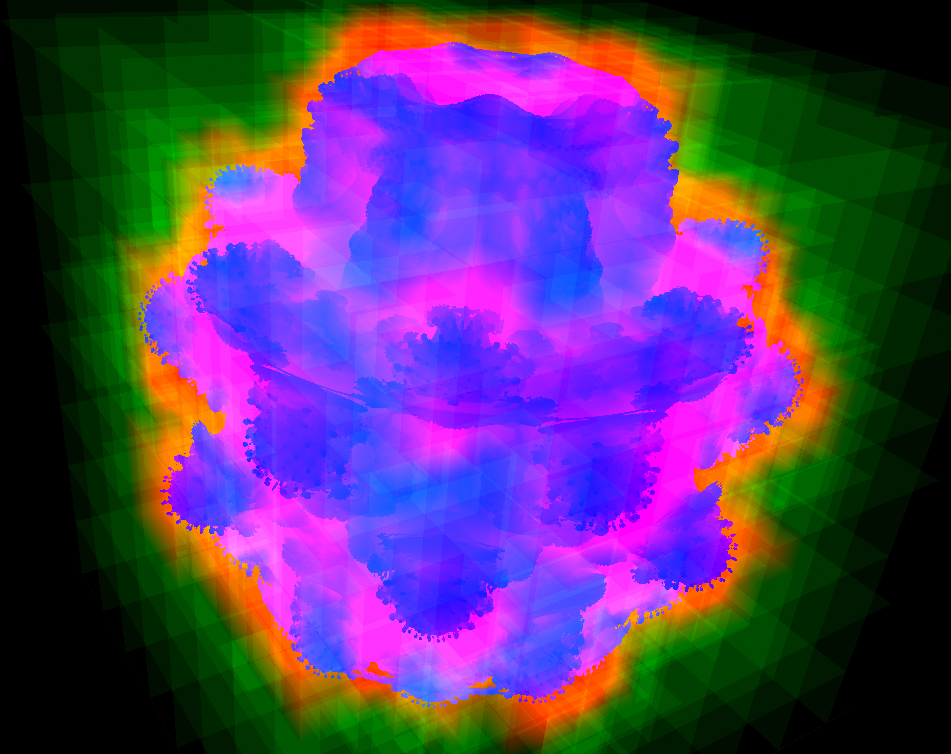
\includegraphics[width=0.95\linewidth]{images/rg/terminate-empty.png}
  \caption{Volume rendering behavior for the Mandelbulb dataset.
  Green indicates bricks that were skipped via empty space skipping.
  Red indicates bricks that were sampled densely.  Blue indicates
  bricks that were sampled but saturated quickly.
%  Most rays skip almost all of the data or terminate very quickly;
%  the lack of white regions in this rendering indicate that, here,
%  \emph{all} rays fall into a single category.
  }
  \label{figrg:bricks-empty}
\end{figure}

\begin{figure*}
  \centering
  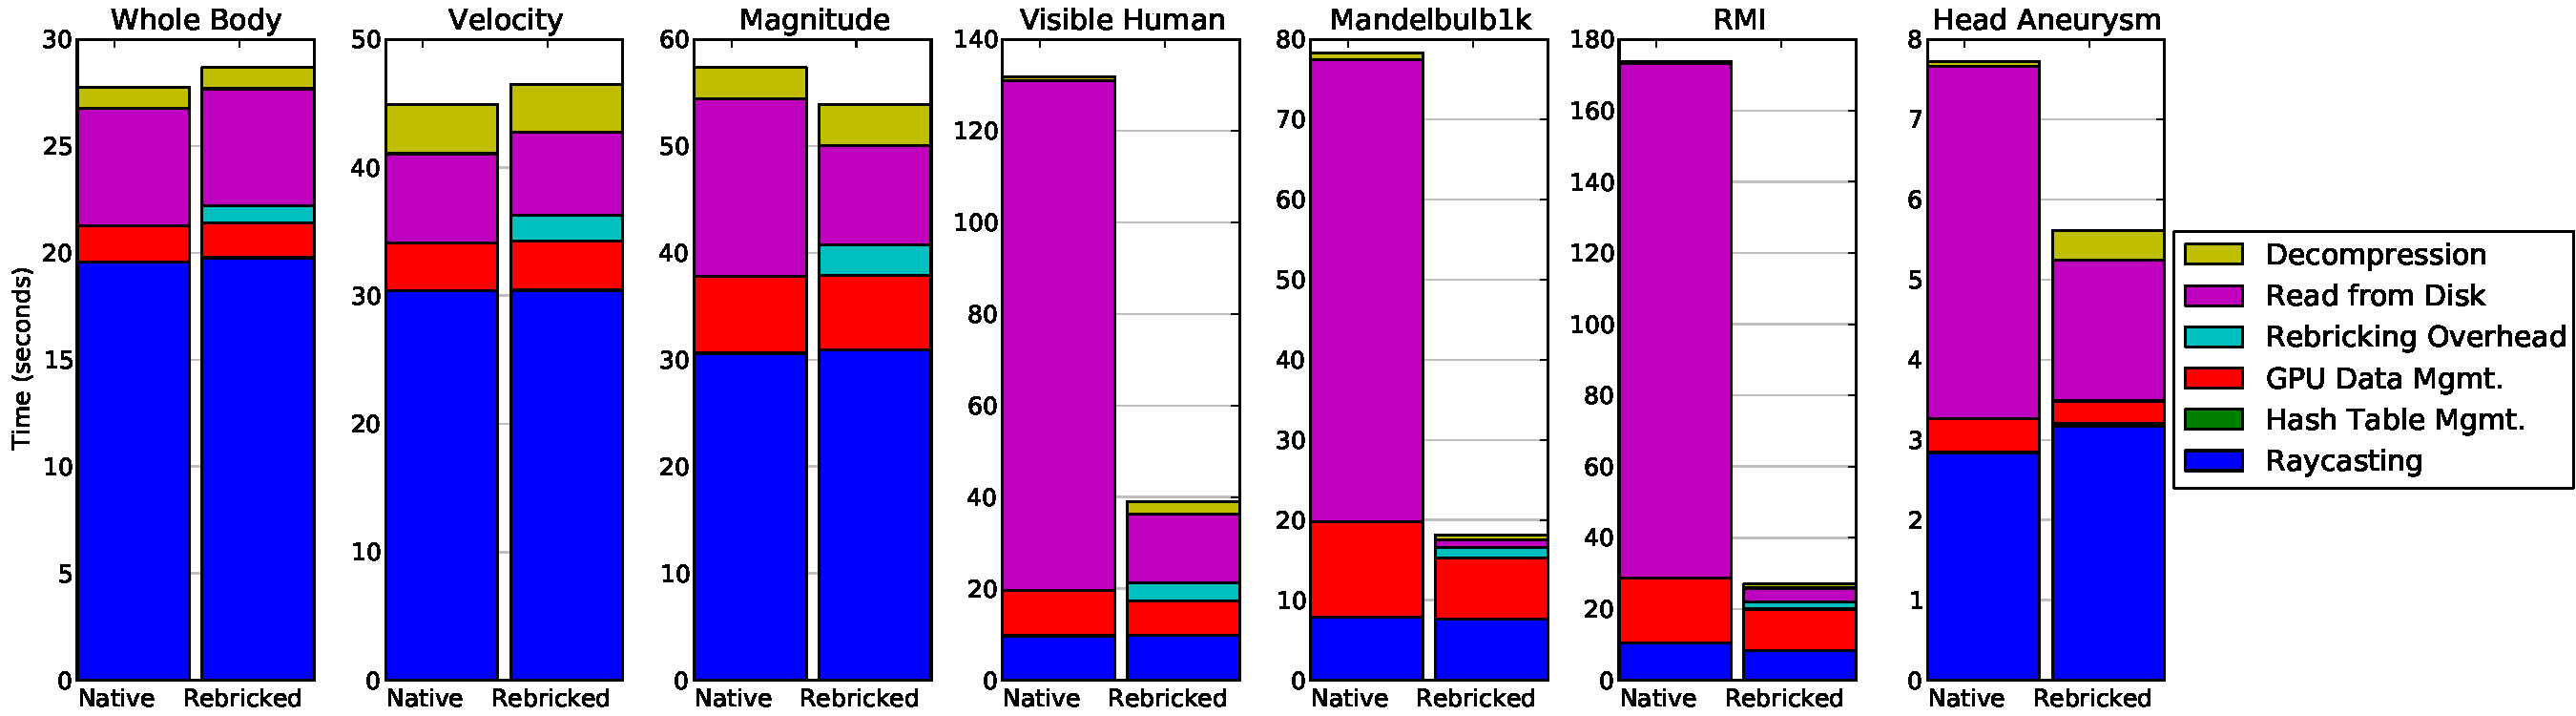
\includegraphics[width=1.00\linewidth]{images/rg/breakdown.pdf}

  \caption{Time spent at various stages of our pipeline, aggregated
  over the generation of a rotation sequence.  Comparisons are made
  between data stored with the ideal brick size for that dataset
  (`Native'), and data stored at a large brick size of $256^3$ with
  the ideally-sized bricks created at run-time (`Rebricked').  `Whole
  Body', `Velocity', and `Magnitude' suffer from a lack of ray
  saturation.}

  \label{figrg:breakdown}
\end{figure*}

\subsection{Brick Classification}
\label{sec:brick-classification}

Considering our target goals (1) through (3) given at the beginning of
this section, one could classify a brick into one of three categories:
\begin{itemize}
  \itemsep0em
  \item skipped due to empty space skipping,

  \item early termination due to ray saturation, or

  \item sampled densely without saturating.
\end{itemize}

An important observation is that---in a very large number of
cases---bricks fall into \emph{either} the `empty' or `saturating'
categories, and only \emph{rarely} in the `non-saturating' category.
The factor that has the greatest effect on performance is how quickly
a renderer can classify data into one of the first two categories, and
therefore bypass a large set of the work.

To make this identification effective, ray-guided volume renderers
maintain the state of each brick, shared on both the GPU and host
memories.  During rendering, one uses the table to identify if a brick
is empty.  If so, the renderer leaps over that space instead.  We store
this as an array consisting of one 32-bit integer per brick of the
dataset.

Figure \ref{figrg:bricks-empty} visualizes this classification for a
large dataset under a typical view and transfer function.  As shown
there, the majority of the visualization falls into either the `blue'
(saturated quickly) or `green' (skipped) sets. This also demonstrates
how little data is actually required for a typical volume rendering.  A
similar rendering is given in the rightmost image of
Figure~\ref{figrg:teaser}, in which only the rays in the middle of the
volume require high computation.

Of course, this classification depends largely on the transfer function
and viewing parameters.  In practice, however, transfer functions that
produce \emph{informative} visualizations tend to exhibit such ternary
classifications.

When the transfer function is changed, this metadata information
must be recomputed.  For datasets with many bricks, this can induce
a noticeable delay.  Our current test platform can process about
7.5 million bricks per second, but even a 1 second delay between
interactions is too much.  Therefore, we offload this update to a
background thread.  Until the thread completes its work, the renderer
considers all unprocessed bricks to be `missing', causing it to request
bricks that might be empty.  Those bricks' metadata are directly
updated and they are only loaded if they fail the empty check.  The
overall performance effects may be large, but the system remains
responsive during this period.

\section{Performance}
\label{sec:performance}

In this section, we give an overview of the various stages of the
renderer and how they perform.  Unless otherwise noted, all timings
were performed on a dual quad-core Xeon 2.2~GHz system using an NVIDIA
GeForce GTX 680, with 24~GB of system memory and 4~GB of GPU memory.
We mostly report results from commodity hard drives, explicitly noting
some specific relevant uses of SSDs.  In many cases, results were
obtained from multiple screen resolutions, but we report results from
an HD viewport ($1920\times1080$) unless noted otherwise.  Details of
the data utilized and renderer timings are given in
Appendix~\ref{sec:data}.

\subsection{Benchmarks}

We have chosen a variety of benchmarks to evaluate the performance of
our renderer, and we elucidate the logic behind those choices here.
First, the choice of HD resolution is motivated by voxel-to-pixel error
ratios.  All modern high-performance volume renderers try to maintain a
1-to-1 ratio between projected voxels and pixels.  Adaptive resolution
selection is used to ensure this ratio.  Without this feature, results
will be aliased, too much information will be compressed to a single
pixel, and performance will suffer.  Adaptive resolution means that
small viewports will not stress renderers: a 512$\times$512 viewport
can get along fine with a paltry few hundred megabytes of memory,
irrespective of the input dataset size.

We utilize zoom-ins, as in the accompanying video and results such as
those in Figure~\ref{figrg:working-set} and some in
Table~\ref{tbl:timings}, to accentuate these high resolution issues.
When the volume is far away, a very coarse resolution is utilized that
maintains accurate voxel-to-pixel error ratios.  As the camera comes
closer, higher resolutions of the source data must be utilized.  We
terminate zoom-ins slightly after they fill the screen; beyond this
point, frustum culling's effect dominates (see
Figure~\ref{figrg:working-set}).  The most challenging cases for a
volume renderer are when data are close enough to be seen at native
resolution, but far enough away that no data can be culled by the
frustum.

Rotations are used to demonstrate that the renderer does not rely
solely on early ray termination.  As described in
Section~\ref{sec:brick-classification} and depicted in
Figure~\ref{figrg:bricks-empty}, most rays either skip large parts of
the volume, or terminate very quickly.  With a transfer function that
produces a dense volume, bricks in the front will prevent bricks in the
rear from ever being paged in, effectively meaning the volume renderer
need only cope with the front \emph{half} or even less of the volume.
Barring pathological volumes and transfer function choices, rotations
ensure all of the data has a chance to contribute to a sequence.

\paragraph{Transfer functions.} Changing a transfer function is also
an important benchmark in any volume rendering system.  Doing so
invalidates our brick metadata concerning which bricks are empty,
causing some hash table entries in the next frame to make little sense
(i.e. request bricks that are visible under the old transfer function
but empty under the new one).  Furthermore, the bricks in the GPU
volume pool may be inappropriate for the new transfer function.

Renderer performance as measured by response time during such an
interaction actually changes very little, and can even improve.
However, quality suffers rather drastically.  This is evident in the
time to convergence after a change in the transfer function: in a
typical case with the RMI data set (see Section~\ref{sec:data}), time
to convergence increased over 6x after changing the transfer function
(from $\sim$380ms to $\sim$2300ms).

\begin{figure*}
  \centering
  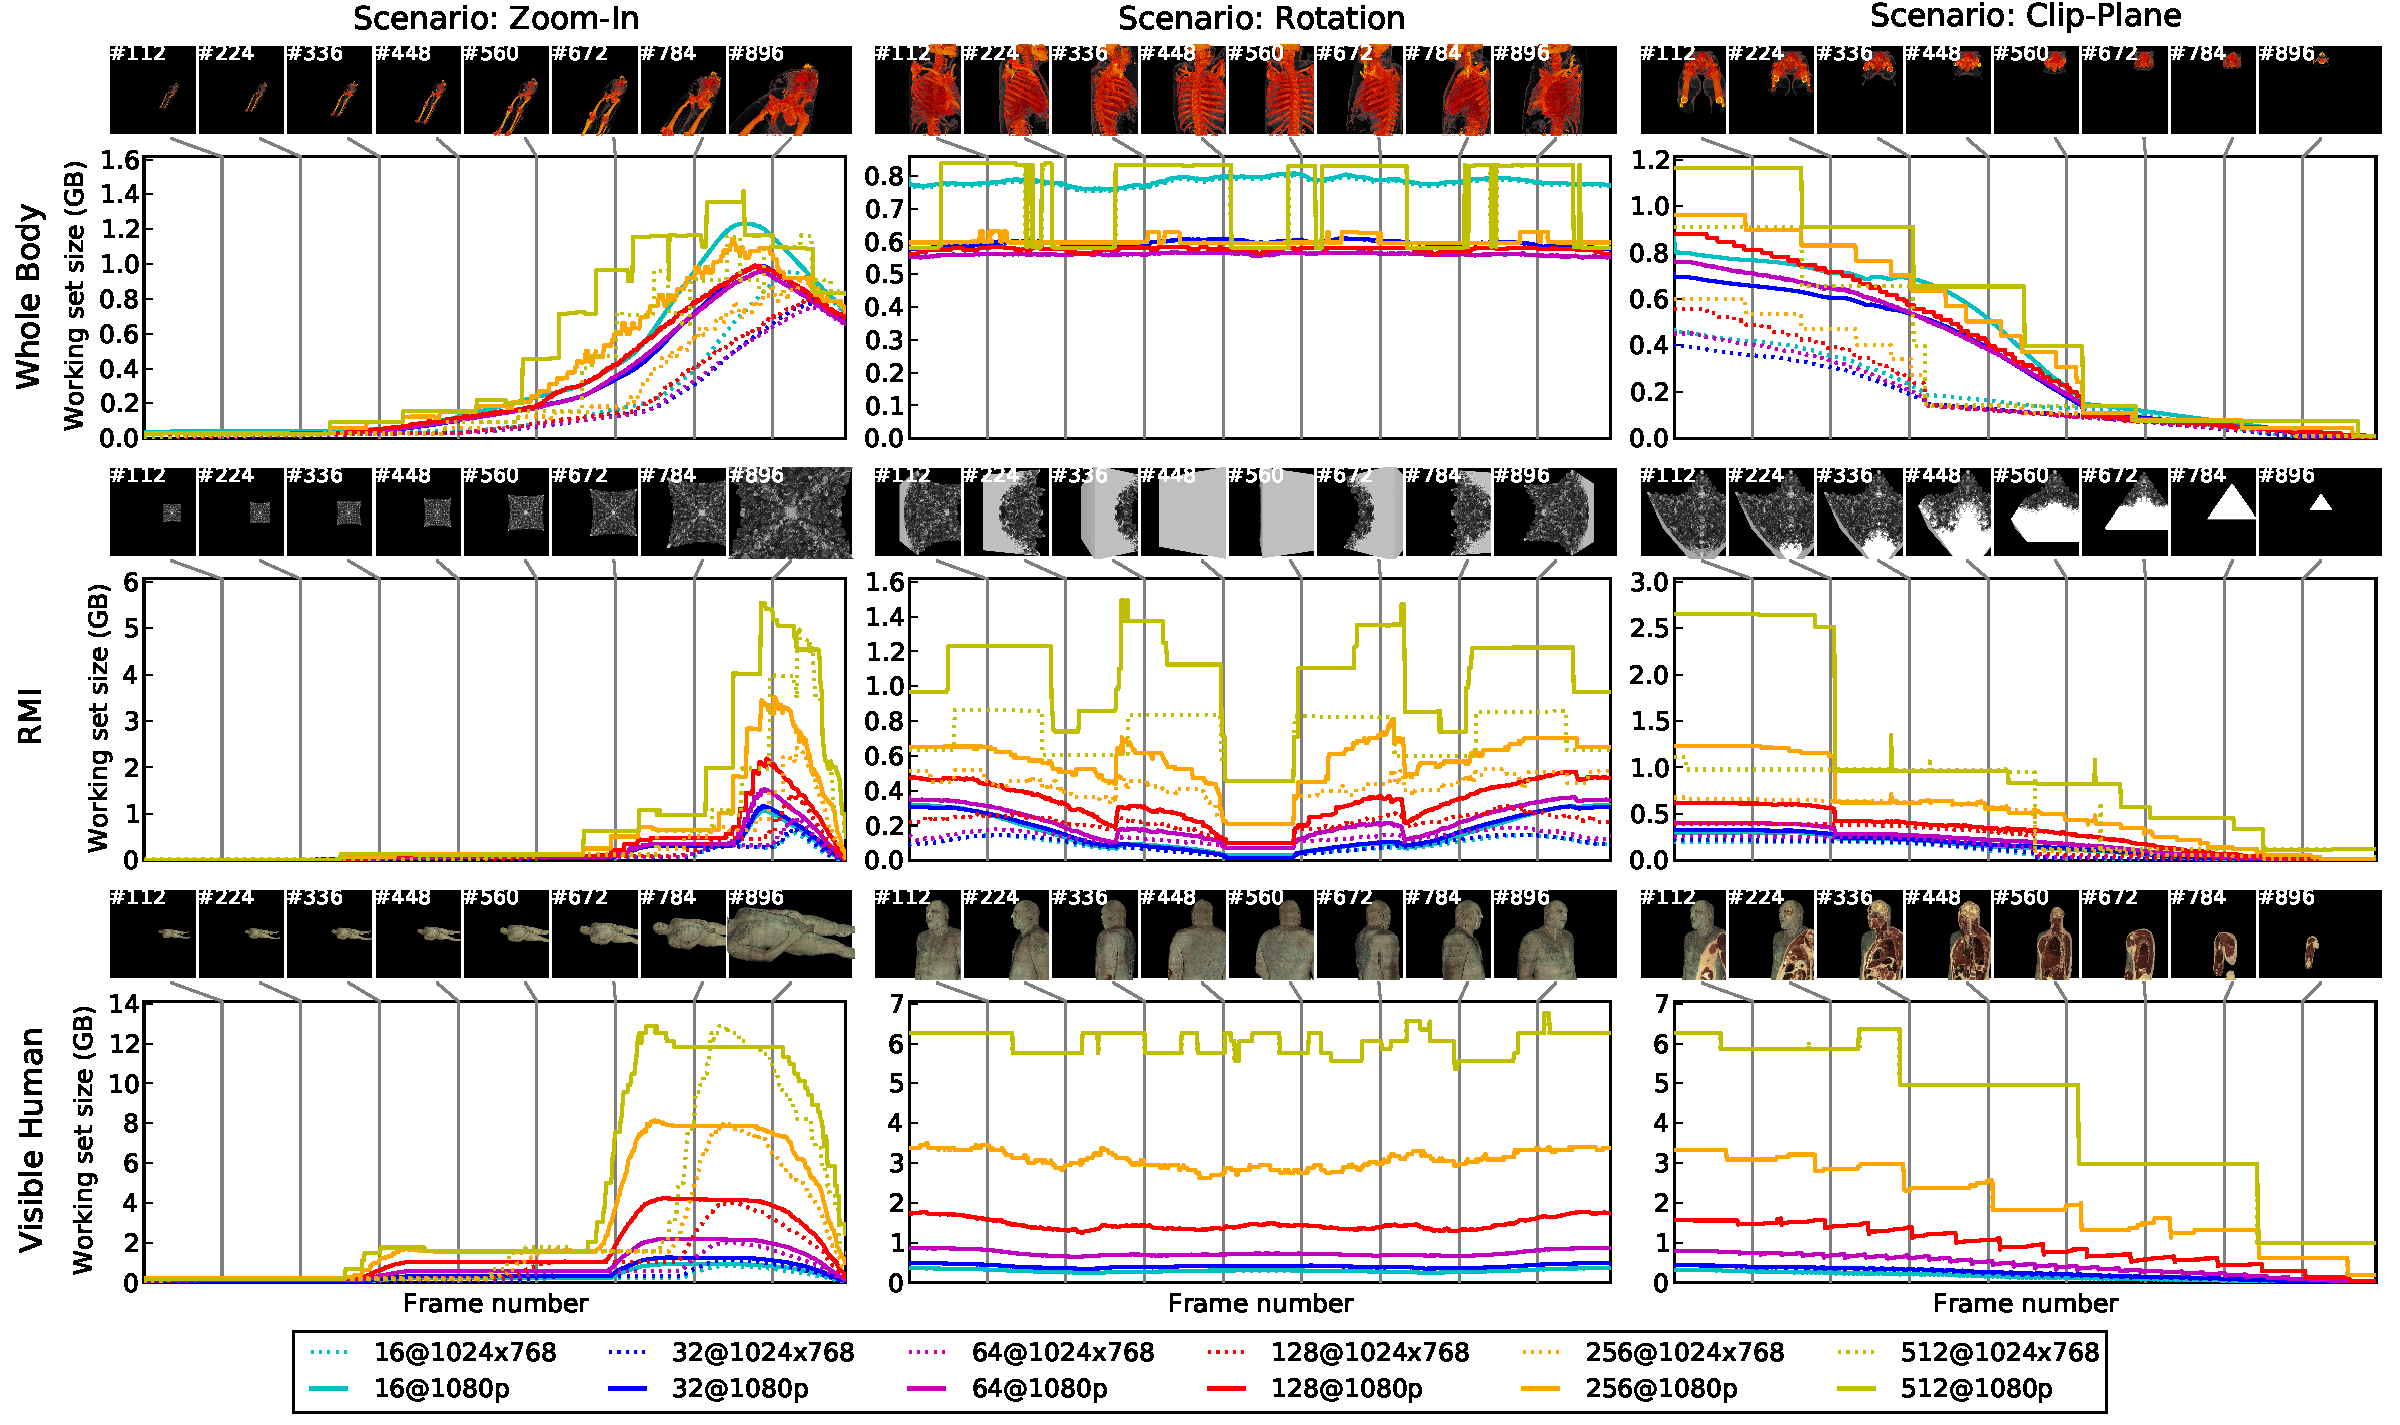
\includegraphics[width=0.98\linewidth]{images/rg/workingSets1-150dpi.pdf}
  \caption{Working set sizes across three different scenarios for
  multiple datasets.  Smaller brick sizes approximate the working set
  better.}
  \label{figrg:working-set}
\end{figure*}

\subsection{Results}
\label{sec:results}

To evaluate our renderer in different scenarios, we used a standard
rotation scenario with a variety of datasets, measuring the length of
each pipeline stage.  Figure~\ref{figrg:breakdown} has these results.  As
IO is the prime bottleneck in many cases, we implemented a `rebricking'
scheme to mitigate the amount of IO performed.  Using large reads and
caching, this significantly lowers the time spent doing IO.  We used
`LZ4' compression when recording this performance data, which trades
CPU time for IO time.

The majority of the time is spent ray-casting, pulling data from disk,
and uploading the bricks to the pool.  Our novel hash table approach
keeps the table small, and so reading it is very cheap: even for large
data, this component does not factor in to the overall performance.
The other GPU data to manage is metadata information for our volume
pool (i.e. which bricks are resident), but at a single machine word per
brick it costs very little to push it down to the GPU, even for very
large data.

Interestingly, the time spent managing GPU data is an increasing
function of volume size \emph{until} it peaks around the size of the
RMI ($2048\times2048\times1920$).  This reinforces our assertion that
there is only so much data visible in a given frame---dependent only on
the view
frustum, and \emph{not} the dataset size---and so at some point we
saturate the set of visible data.  Figure~\ref{figrg:working-set} and
Section~\ref{sec:subdivision} include more discussion about working set
sizes.

% \todo{datasets to beat/compare with:
% 2048x1024x1080, 16bit, 640x480 viewport: 95 minutes to preprocess
% ($32^3$). biomedical data (lizard scan?).  12 to 30 Hz range; avg 16 Hz
% for volume rendering, avg 20 Hz for
% iso. dvr had peak memory use of: 153.125 megabytes\cite{Gobbetti:2008:VR}.\\
% 21494x25790x1850, 1024x768 viewport. ``mouse cortex''. two transfer
% functions: one runs at 75 Hz, another at 12.\cite{Beyer:2012:DSM}\\
% 18000x18000x304, 1024x768 viewport.  77 Hz and 19
% Hz\cite{Beyer:2012:DSM}.\\
% $2048^3$, 1024x768 viewport.  55 and 30 Hz.\cite{Beyer:2012:DSM}.
% }

\section{Design Tradeoffs}
\label{sec:tradeoffs}

In this section, we try to explore aspects that have not been
thoroughly addressed by previous literature.  Details on trade-offs and
the reasoning behind our final implementation choices are given.

% There are a variety of considerations in a ray-guided volume renderer
% which have not been thoroughly addressed in previous literature.  We
% endeavor to explore some of these choices here, and explicitly detail
% the inherent trade-offs and reasoning behind our final decisions.

\subsection{Subdivision}
\label{sec:subdivision}

How a system subdivides the volume into manageable pieces can have
a large effect on the performance of the renderer.  The primary
considerations are in regard to early ray termination and empty space
skipping: small bricks are much more likely to be composed of a small
range or even uniform values, which will make it more likely that the
brick can be skipped under a large set of transfer functions.  Further,
small bricks means one will detect ray saturation much more quickly, as
this is checked only when exiting a brick.

\paragraph{Internal Overhead}

The primary drawback is reduced disk throughput due to utilizing many
small requests.  A further drawback is the data size overhead: each
brick needs two voxels of ghost data in each dimension, for sampling
and gradient computation purposes.  This is negligible for large
bricks, but grows sharply as the brick size approaches one, as shown in
Figure
\ref{figrg:brick-size}. Figure~\ref{figrg:hierarchy-build} demonstrates
that this is not strictly a theoretical result: a small brick size
greatly increases not just size overhead, but also the time to
reorganize the data on disk.  From these Figures we can derive that for
large datasets a brick size of less than $16^3$ is impractical.

\paragraph{External Overhead}

We have performed a number of experiments to identify the working set
size for multiple different brick sizes.  Starting with the smallest
practical size of $16^3$, we increase the brick size up to $512^3$.

As can be seen in Figure~\ref{figrg:working-set} the working set is bound
not by just the data size, but the screen resolution as well.  It can
also be seen that the brick size heavily influences the working set
size: larger bricks allow for less efficient utilization of empty
regions. From the images we can derive that a brick size of less than
$128^3$ is desirable to reduce the working set to roughly the memory
size of a GPU.

We note that the working set size is not a strict function of the brick
size, however.  Figure~\ref{figrg:working-set} and
Table~\ref{tbl:timings} also show that the choice of brick size is not
clear-cut.  The Visible Human male performs best with $16^3$ bricks,
for example, whereas the ideal brick size for the `Magnitude' data is
$64^3$.  For the `Whole Body' dataset, using brick sizes of
$16^3$ actually resulted in \emph{larger} working sets than $32^3$.
This occurs when the transfer function produces large regions
of semi-transparency but never reaches saturation.  Indeed, when datasets
contain large swaths of semi-transparent regions, the conventional
wisdom is reversed: large brick sizes are generally preferred, since
they significantly improve disk throughput.

% \paragraph{Performance}
%
% There are three primary metrics to be concerned with when evaluating
% a volume renderer's performance.  One of them is the commonly
% evaluated metric: the time required to render the data at the
% required resolution.  The second is system responsiveness: if the
% user changes a viewing parameter, a transfer function, or any other
% state, the renderer should respond quickly.  A third consideration is
% the time to generate these data: converting a large dataset into a
% bricked representation grows sharply as the brick size shrinks.
%
% \todo{table or graph of brick size (X) and `time to build hierarchy' (Y)}

%% moved this up into other paragraph
% As can be seen Table \ref{tbl:timings} and Figure
% \ref{figrg:working-set}, the brick size choice is not clear-cut.
%   The
% Visible Human male performs best with $16^3$ bricks, for example,
% whereas the ideal brick size for the `Magnitude' data is $64^3$.  When
% the transfer function keeps large regions mostly transparent, as is the
% case for the `Whole Body' and `Velocity' datasets, then the improved IO
% performance gleaned from large requests derives the most benefit.

If we begin to consider secondary metrics, such as the response time of
the system, the choice of brick size becomes even more complex.  Since
bricks are the atomic building blocks in a volume renderer, one cannot
load less than a single brick from disk. Therefore a larger brick size
imposes a larger response time on the system.  These concerns would
generally push a designer to choose smaller bricks.

However, disk performance falls very sharply with small
requests~\cite{Fogal:2011:PracticalIO}.  It is nice for a system to
respond within a few tens of milliseconds, but such concerns should not
dictate the design to the point that end-to-end performance suffers
drastically.  Furthermore, small brick sizes are accompanied with
significant
overhead, as discussed in Figure \ref{figrg:brick-size}, and do not
compress as effectively as their larger counterparts.

Systems such as Reichl et al.'s hybrid surface rendering, CERA-TVR, and
Gigavoxels utilize a static brick size of
$32^3$~\cite{Reichl:2012:HybridSurface, Engel:2012:CERA,
Crassin:2009:Gigavoxels}.  This brick size exhibits few extremes of the
performance issues mentioned above. However, it is certainly not the
ideal choice for all circumstances.

\begin{figure}
  \centering
  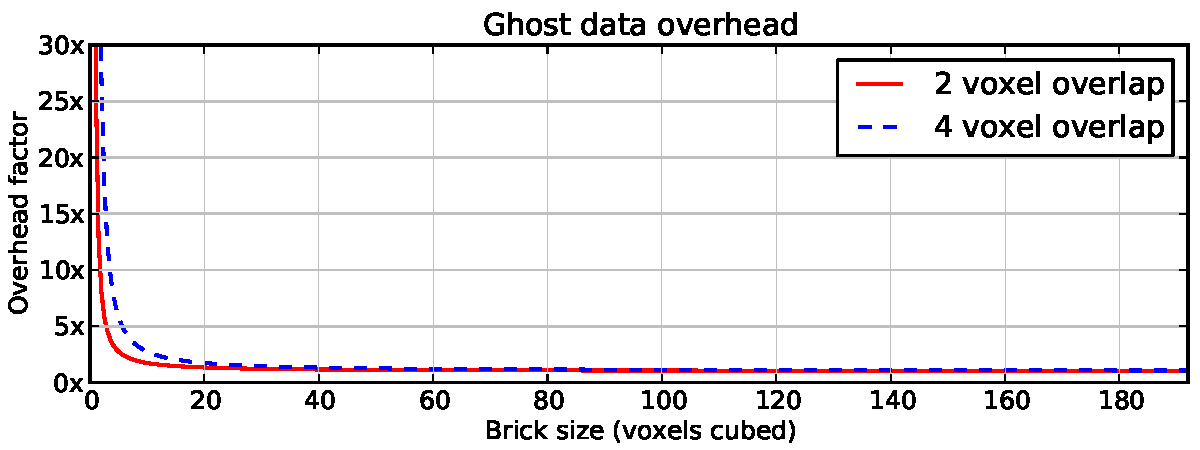
\includegraphics[width=0.99\linewidth]{images/rg/BS-overhead.pdf}
  \caption{Brick size overhead.  As bricks get smaller, the overhead
  for the additional ghost data grows significantly.  At a larger brick
  size of $128^3$, the overhead with 2 ghost voxels per dimension
  amounts to a few percent, whereas with $32^3$ bricks this increases
  the dataset size by almost 50\%.}
  \label{figrg:brick-size}
\end{figure}

\subsection{Disk IO}

\subsubsection{Brick Layout}

Figure~\ref{figrg:layout} demonstrates how this changes with the brick
size.  Both disk IO times as well as decompression times are displayed
there.  As shown in the figure, reading data from disk becomes quite
severe with small brick sizes.  However, as brick sizes grow to $64^3$
and beyond, decompression time becomes more important and overall time
plummets.  This effect is even more pronounced using a hard disk in
place of the SSD used here.  Intelligent layout strategies purport to
minimize seek times; our results corroborate this, with the important
caveat that seek times are not relevant with larger brick sizes.

\begin{figure}[tb]
  \centering
  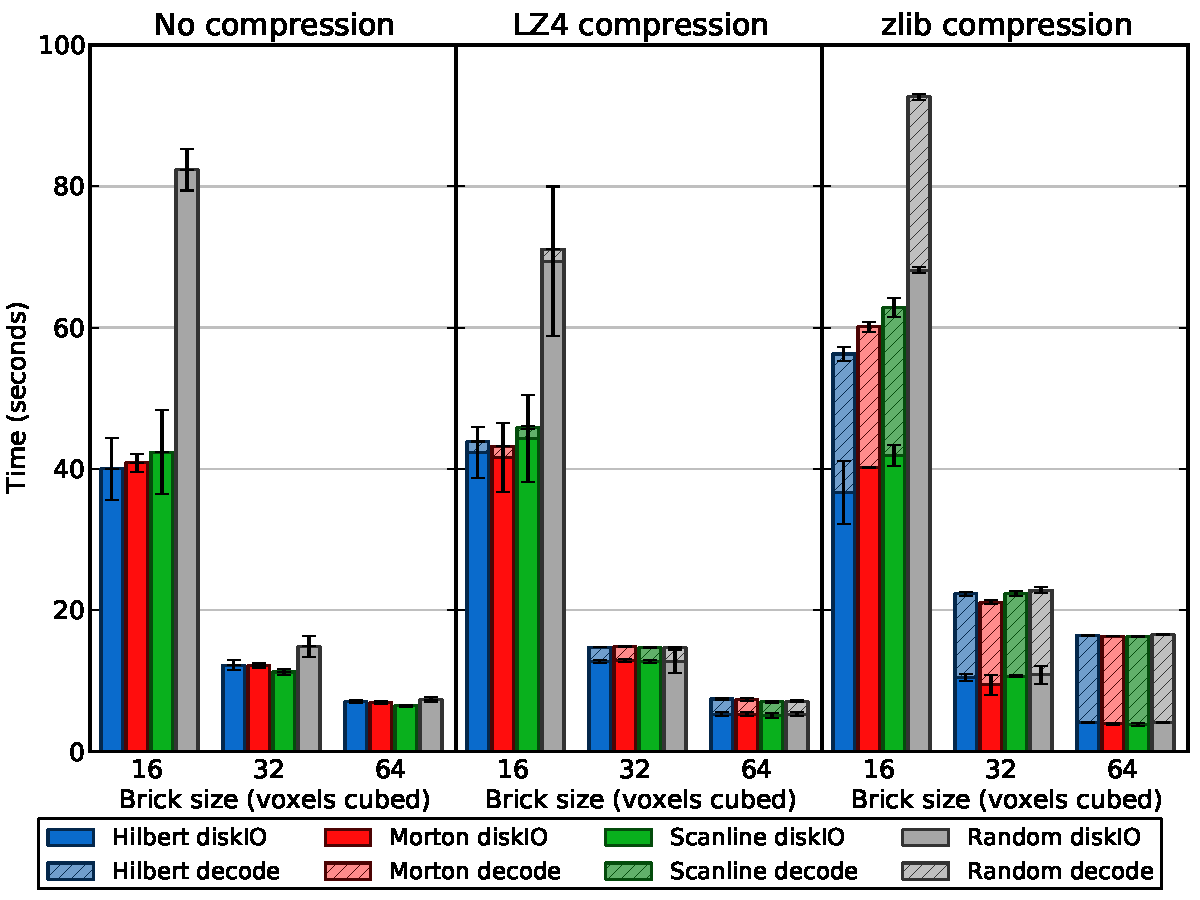
\includegraphics[width=1.00\linewidth]{images/rg/brickIO-RichtmyerMeshkov-ZoomIn-SSD.pdf}

  \caption{Time spent with IO-related tasks using an SSD for the
  RMI dataset's zoom-in scenario, sampled with 100 frames and a
  $1024\times768$ viewport.  Layout strategies only see utility at
  small brick sizes.}

  \label{figrg:layout}
\end{figure}

% \begin{figure}
%   \centering
%   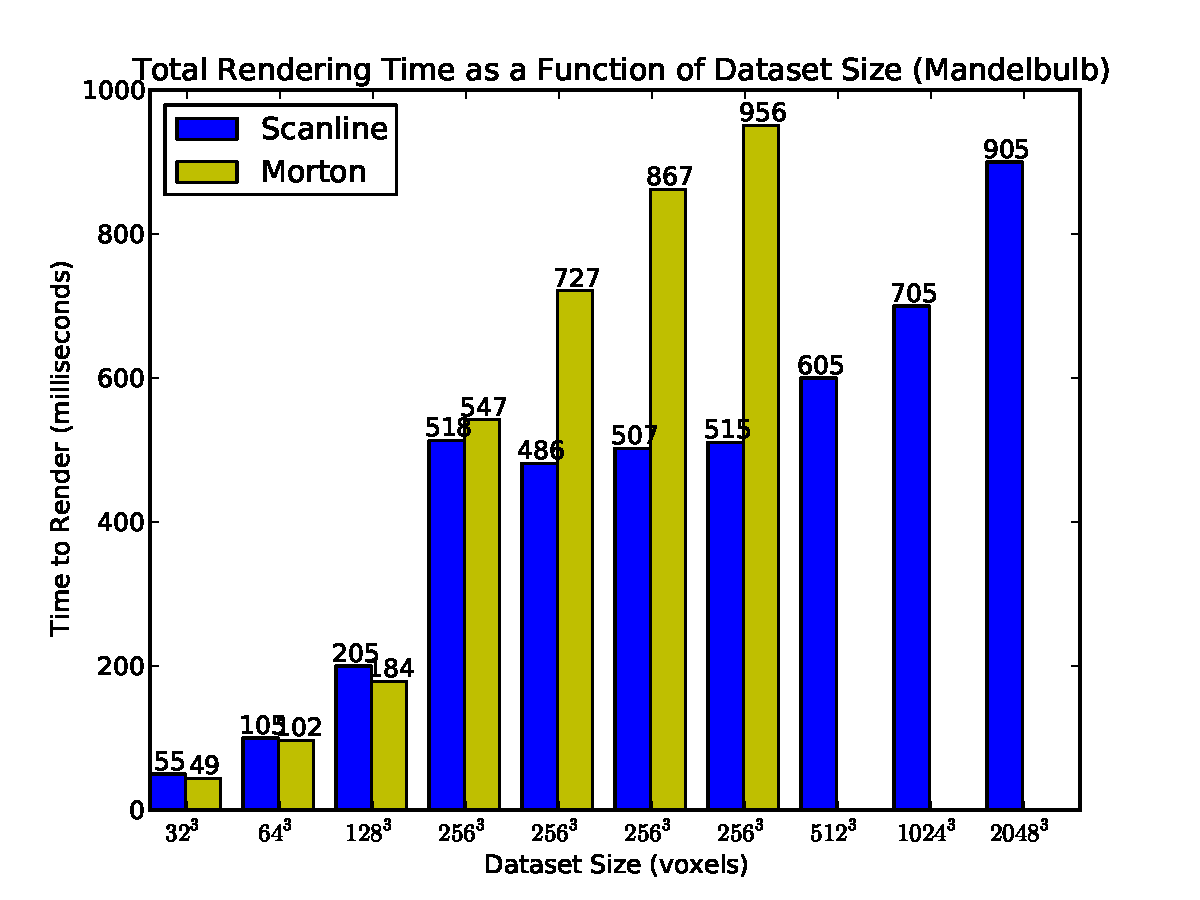
\includegraphics[width=\linewidth]{images/dsize-rtime}
%   \caption{\todo{needs update, data is made up (alex: benchmark! run
%   dsize-performance.lua)} Total rendering time, including brick IO,
%   to generate animations for the `mandelbulb' dataset at various
%   sizes and two distinct layouts.  Brick size was $32^3$ for all
%   runs.  Layout scheme has relatively little impact: disk read time is
%   negligible relative to the entire process.}
%   \label{figrg:rtime-layout}
% \end{figure}

\subsubsection{Dynamic Rebricking}
\label{sec:rebricking}

% \todo{this is too long. important message: rebricking is a good idea,
% because it avoids absurd hierarchy build times and gives good I/O
% performance. the overhead is demonstrably minor.}

The renderer desires small bricks, as discussed in
Section~\ref{sec:subdivision}, as small bricks will help with early ray
termination and empty space leaping.  However Figures~\ref{figrg:layout}
and \ref{figrg:brick-size} clearly demonstrate that large brick sizes
are preferable for disk performance and overhead reasons.  To provide
the best of both worlds, we implemented a `dynamic' bricking scheme,
whereby bricks are stored on disk in a rather large size (e.g. $256^3$)
but presented to the renderer as if they exist at some small resolution
($32^3$).  The small bricks are dynamically generated from the large ones on
request.

Since requesting a large brick for every small brick would only
increase the disk traffic, we keep an additional brick cache in memory
to source these copies from.  Our cache uses a standard LRU strategy.
This is advantageous when the working set of the data fits into the
host memory, however when the working set exceeds the host memory we
will evict entries before finishing a rendering.  We stuck with this
strategy since the working set
often \emph{does} fit into host memory, as established by
Figure~\ref{figrg:working-set}.  If the renderer is to be used in an
environment in which working sets are routinely larger than memory, an
MRU strategy would be more appropriate.

\paragraph{Hierarchy Generation}

Reorganizing data into a set of bricks is mostly ignored in volume
rendering literature, but becomes a significant bottleneck in
real-world usage.
Figure~\ref{figrg:hierarchy-build} shows the time our preprocess needs
to generate this hierarchy, which increases sharply for small brick
sizes.  This time also increases with respect to dataset size.  At
the extreme scale, such data reorganization is completely infeasible:
merely reading every datum might take months.  We believe such
reorganization will be feasible up to a few tens of terabytes.  In
practice, the authors and collaborators thereof tolerate this for up to
4 terabytes at present.

% For the case of visualization-based verification, a dataset might
% only need to be loaded once to identify that a parameter was set
% wrong; this data reorganization is then a very high cost to pay.

Rebricking the data at run time alleviates this problem.  The data can
be generated at very large brick sizes, enabling fast conversion and
effective disk throughput, and then dynamically rebricked to very small
sizes.  Both disk and renderer deal with their ideal cases, then.  The
`Rebricking' case of Figure~\ref{figrg:breakdown} shows performance in
this mode.

%% compression isn't unique enough to have its own story, particularly
%% since we need space.

% \subsubsection{Compression}
% 
% Regular gridded data typically contains large areas of uniform
% values.  One example is in the outer regions: most scanners as well as
% simulation software produce many layers of zeroes outside the region of
% interest.  Especially in simulation output, there may be large areas in
% a dataset which change at a very low frequency, producing runs of the
% same data value. All of these regions compress very effectively.
% 
% \todo{make it clear we are compressing each brick in isolation, storing
% it compressed on disk, and decompressing it when it is read---before it
% makes it to the renderer}
%
% \begin{figure}
%   \centering
%   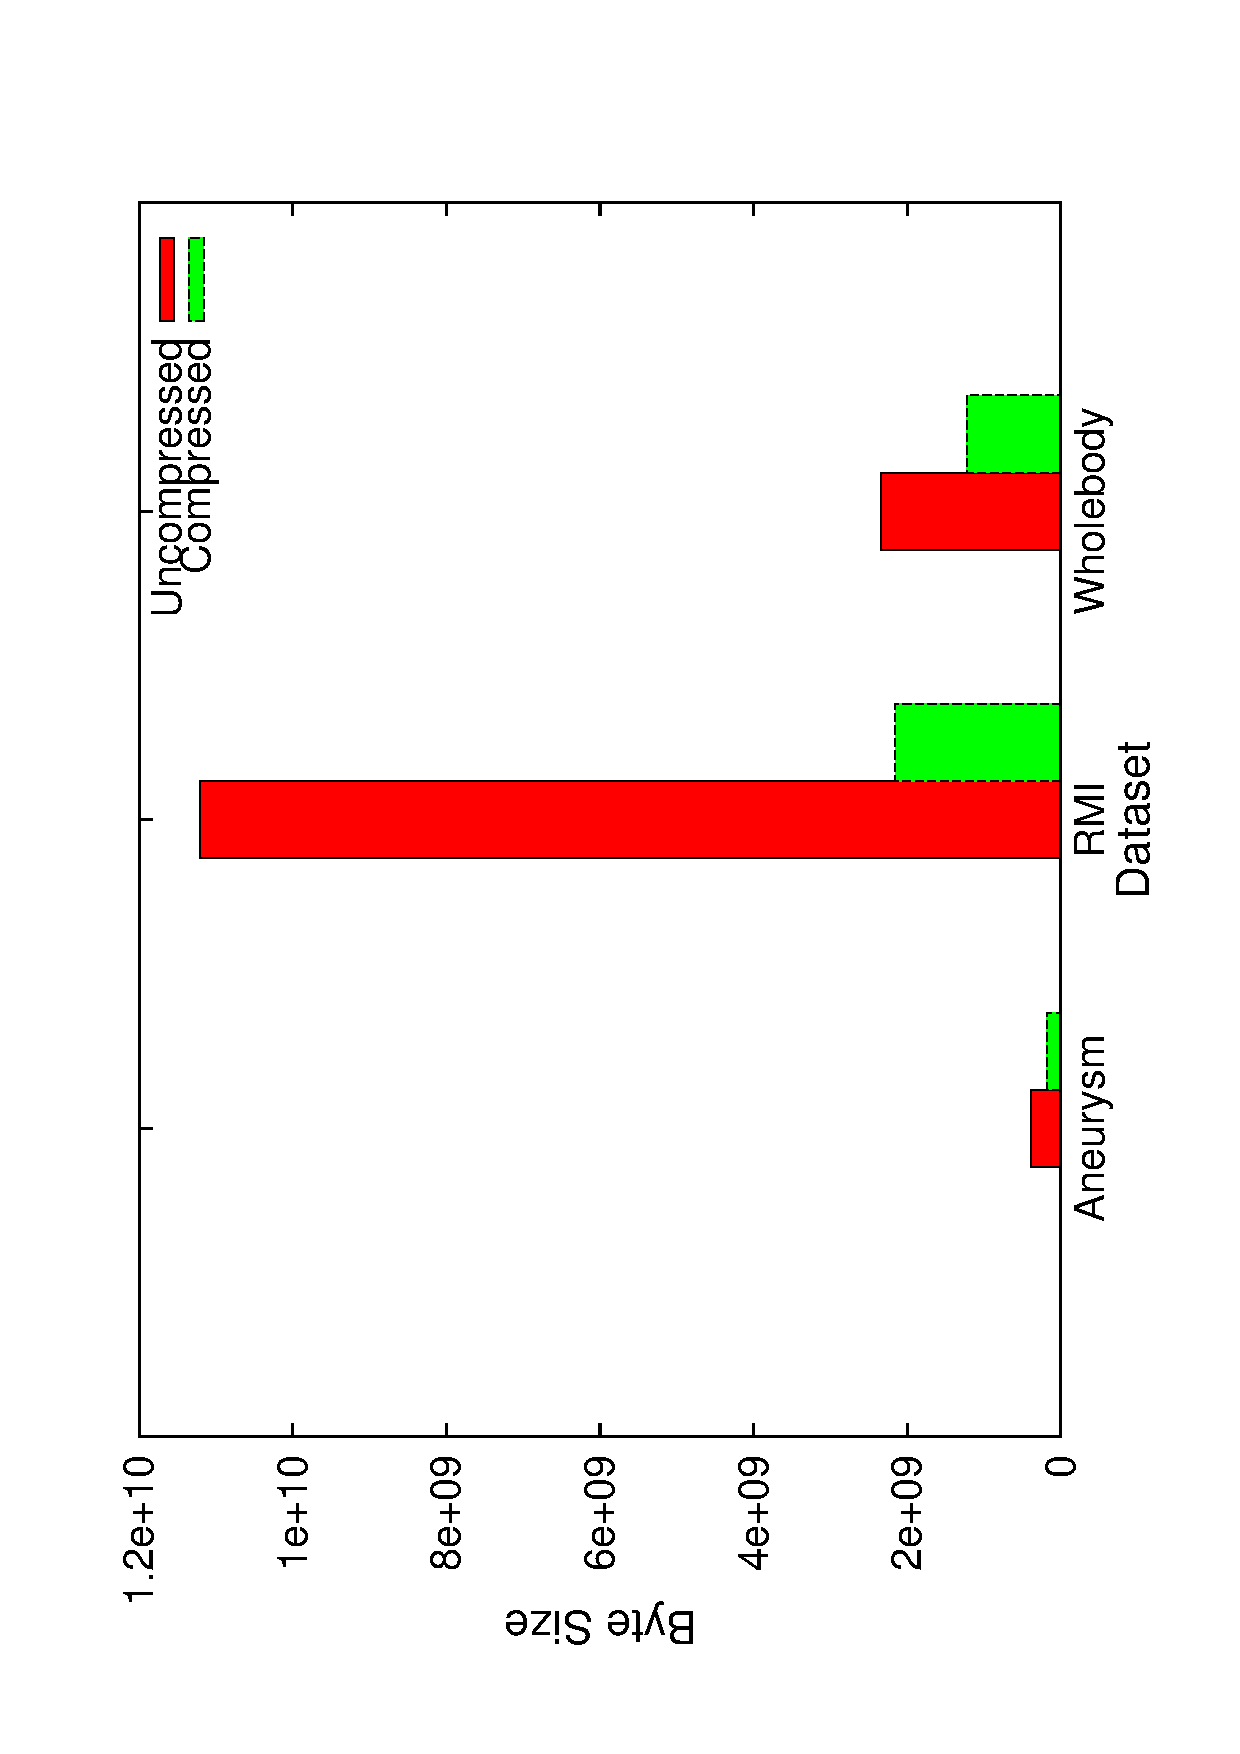
\includegraphics[width=\linewidth]{images/Compression}
%   \caption{Compression ratios for a variety of datasets using the
%   `fastest' zlib compression mode.  Very often, data compress to a
%   factor of less than half their original size. \todo{Alex will replace
%   this graph}}
%   \label{figrg:compression}
% \end{figure}
%
% \todo{Need results for (\emph{many}!) more datasets!}

% The zlib libary has given us very good results for many datasets.
% Some results on the compression ratio are given in Figure
% \ref{figrg:compression}.  Our system compresses data per-brick, and is
% instrumented to keep track of the data sizes both before and after
% compression.  Interestingly, these brick sizes \emph{always} shrink:
% we have not identified a single brick in any depicted (as well as many
% other) datasets for which the post-compression size is increased.  We
% attribute this to the addition of ghost data, which enlarges even the
% smallest brick to $3^3$.

\begin{figure}[tb]
  \centering
  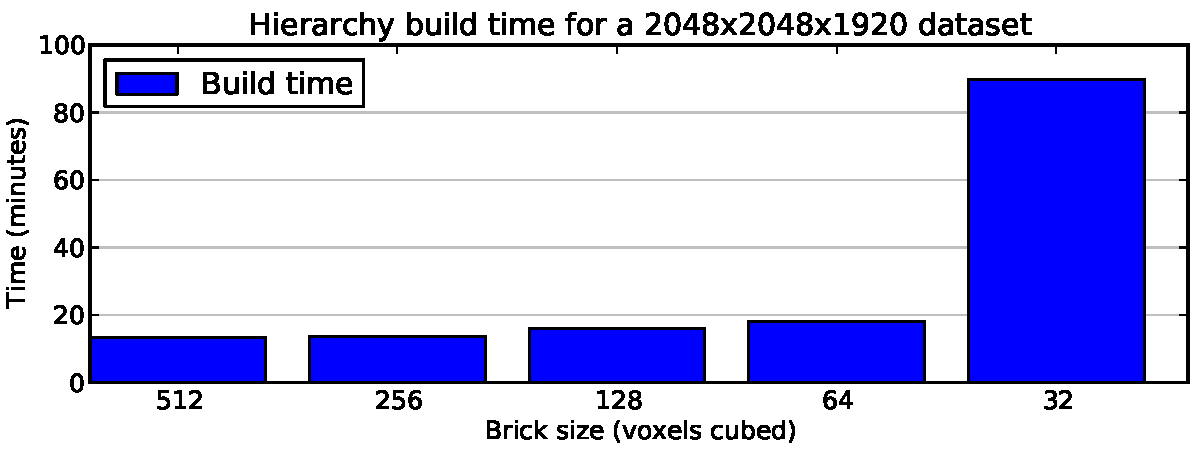
\includegraphics[width=0.98\linewidth]{images/rg/HierarchyBuildTime.pdf}
  \caption{Time to build bricked representation for a medium-sized dataset,
  as a function of brick size.  Renderers desire small bricks to
  perform efficiently, but generating such bricks takes significant
  preprocessing resources.}
  \label{figrg:hierarchy-build}
\end{figure}


\begin{figure*}
  \centering
 \begin{minipage}[t]{0.3651225\linewidth}
   \begin{algorithm}[H]
   \caption{Greedy algorithm: request all bricks at all
   resolutions.\vspace{0.1em}}
     \begin{algorithmic}[H]
     \State ReportMissingBrick(\textit{b}) \Repeat
       \State \textit{LoD++}
       \State \textit{b} = LookupBrick(\textit{ray}, \textit{LoD})
       \If{Missing(\textit{b})}
         \State ReportMissingBrick($b$)
       \EndIf
     \Until{$\lnot$Missing(\textit{b})}\\
     \end{algorithmic}
   \end{algorithm}
 \end{minipage}
 \hfill
 \begin{minipage}[t]{0.55\linewidth}
   \begin{algorithm}[H]
   \caption{Global algorithm: only request bricks required to satisfy
   the final rendering request.\vspace{0.000em}}
     \begin{algorithmic}[0]
       \State ReportMissingBrick(\textit{b})
       \Repeat
         \State \textit{LoD++}
         \State \textit{b} = LookupBrick(\textit{ray}, \textit{LoD})
       \Until{$\lnot$Missing(\textit{b})}
     \end{algorithmic}
   \end{algorithm}
 \end{minipage}

  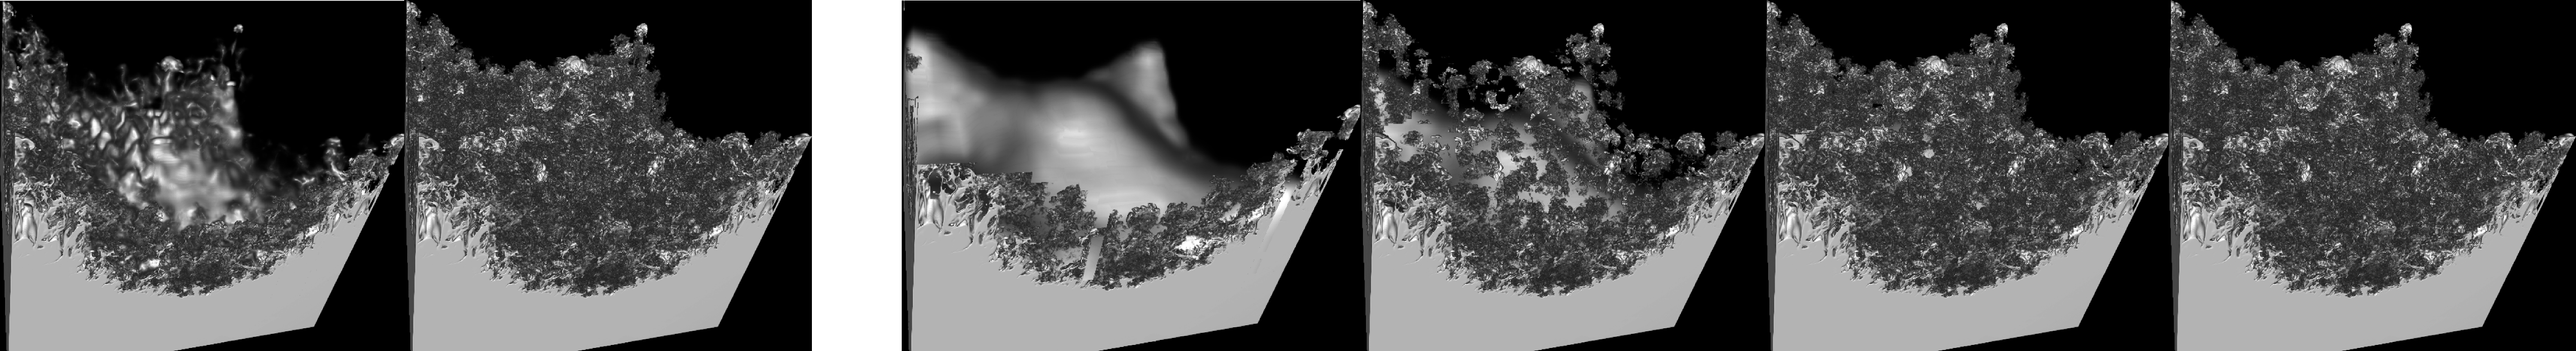
\includegraphics[width=\linewidth]{images/rg/strategy.png}
%   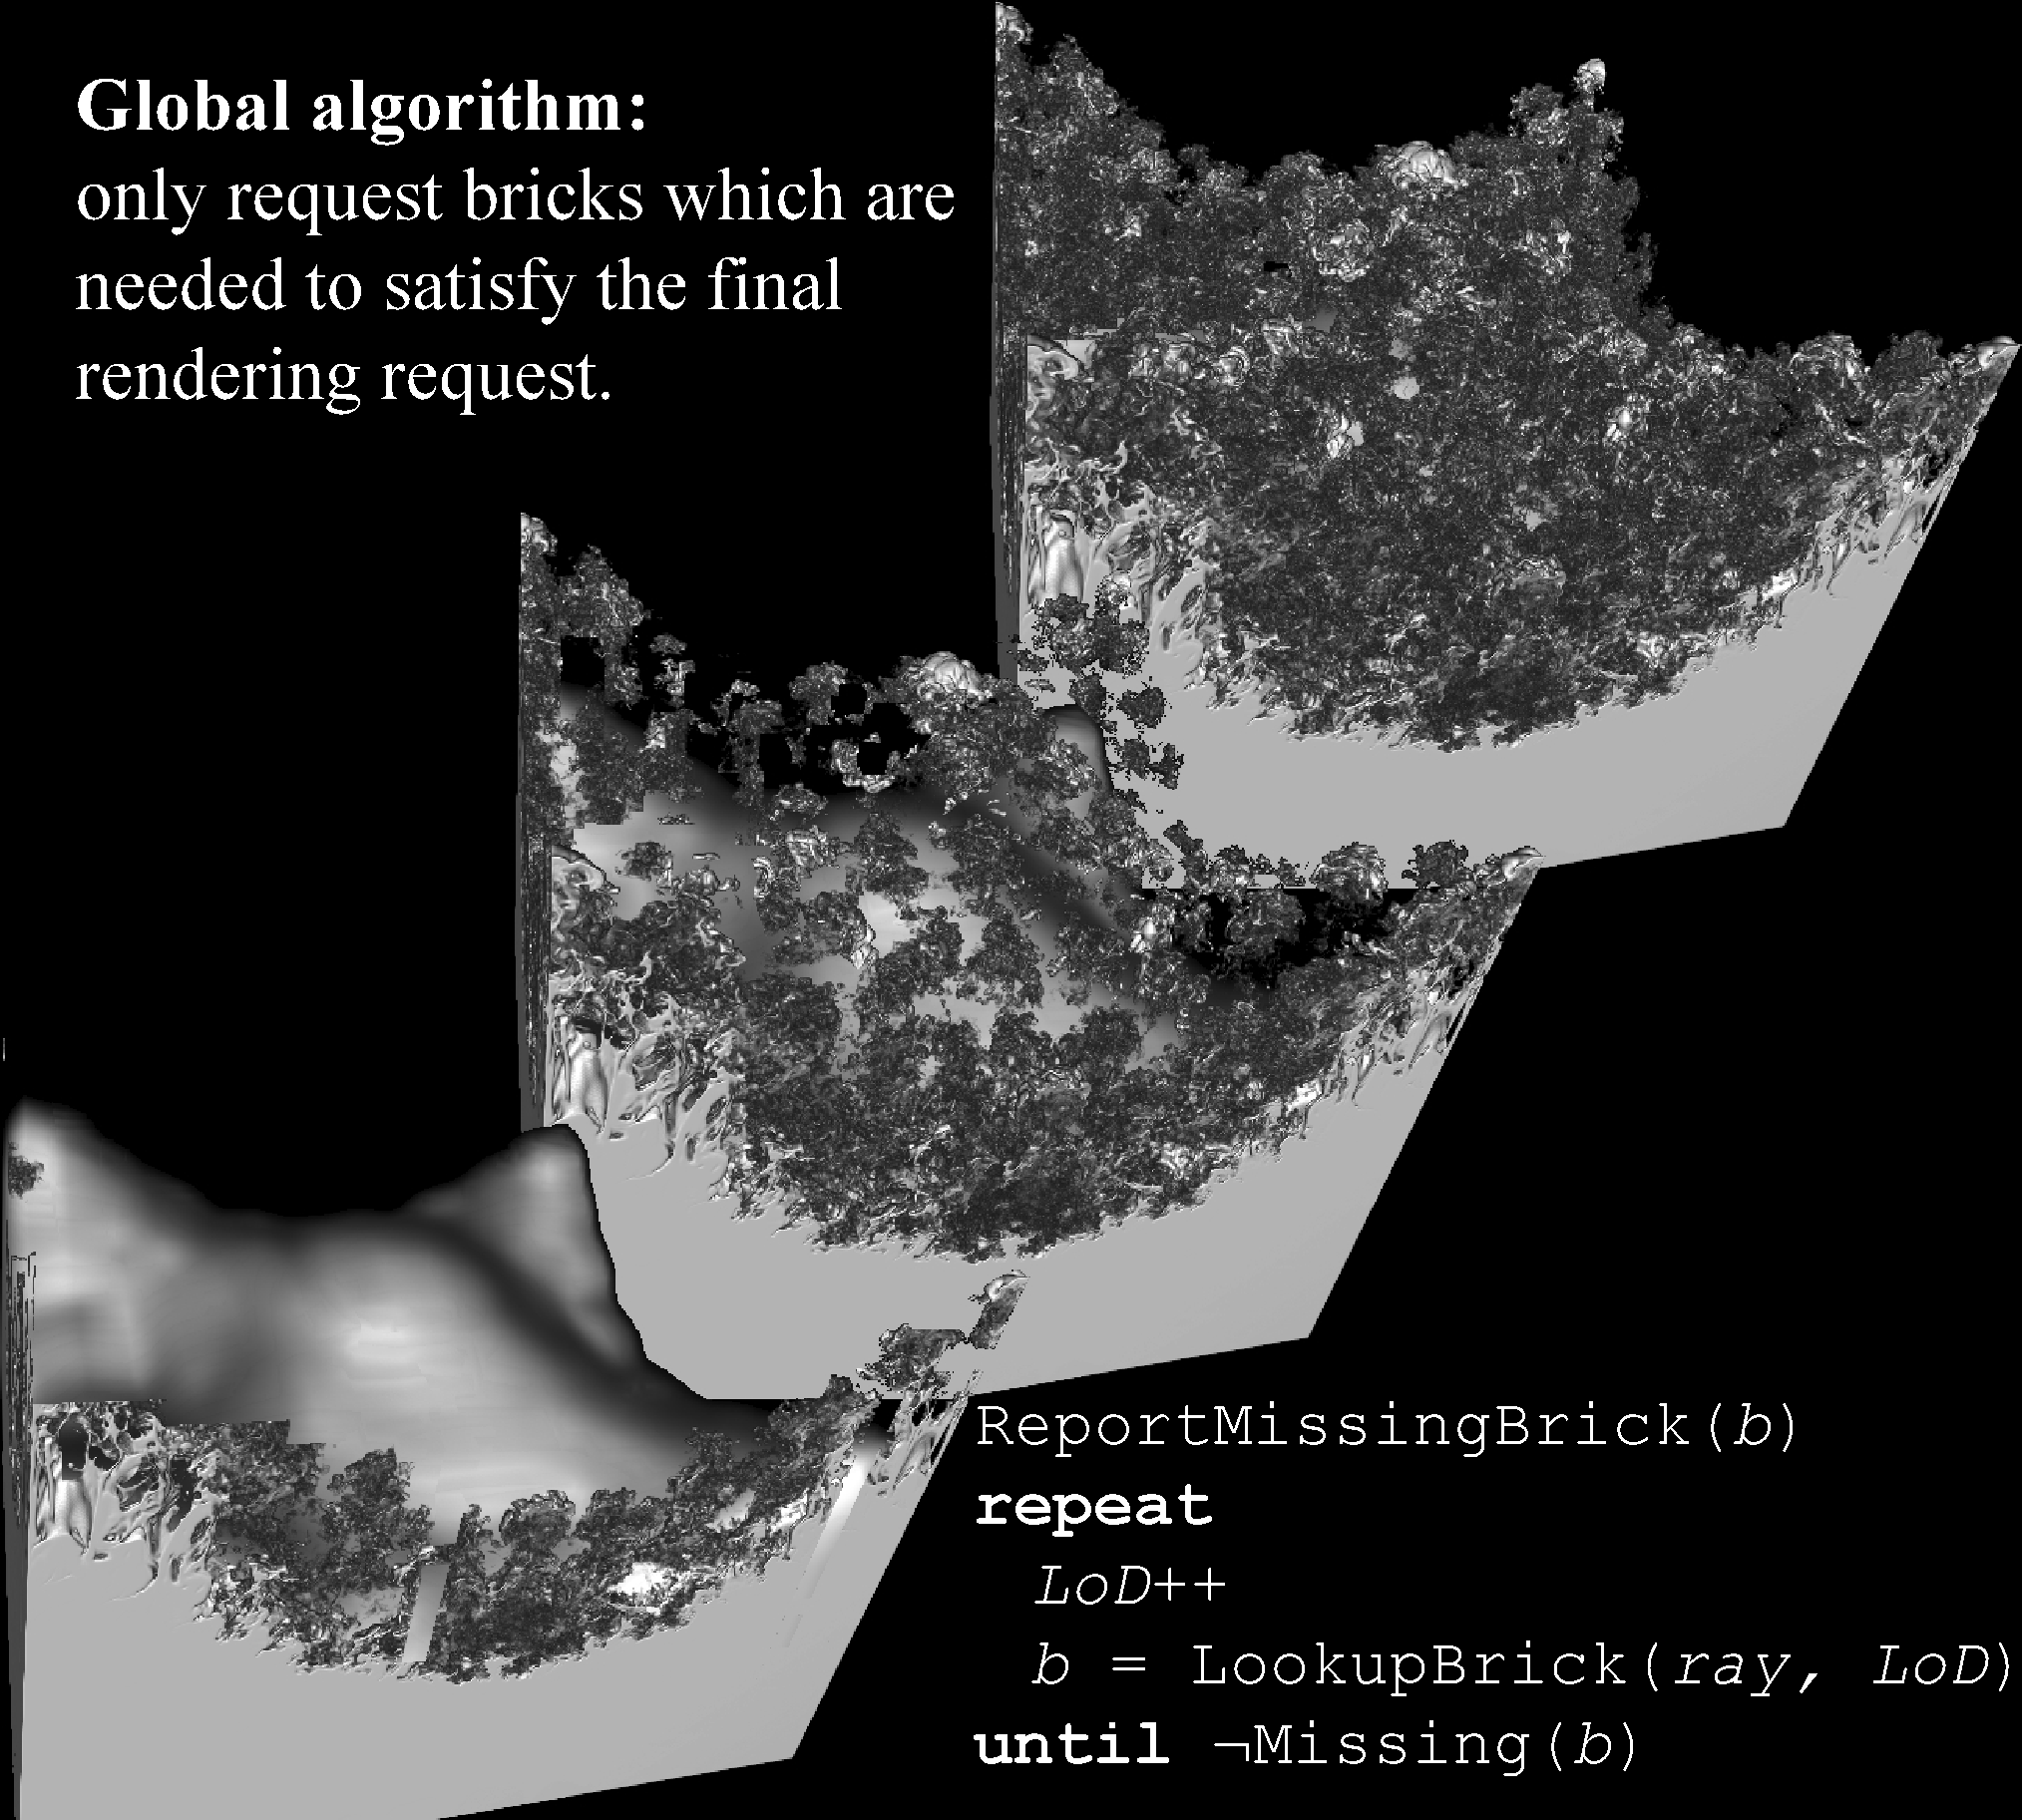
\includegraphics[width=0.99\linewidth]{images/Algorithm-Global}
%   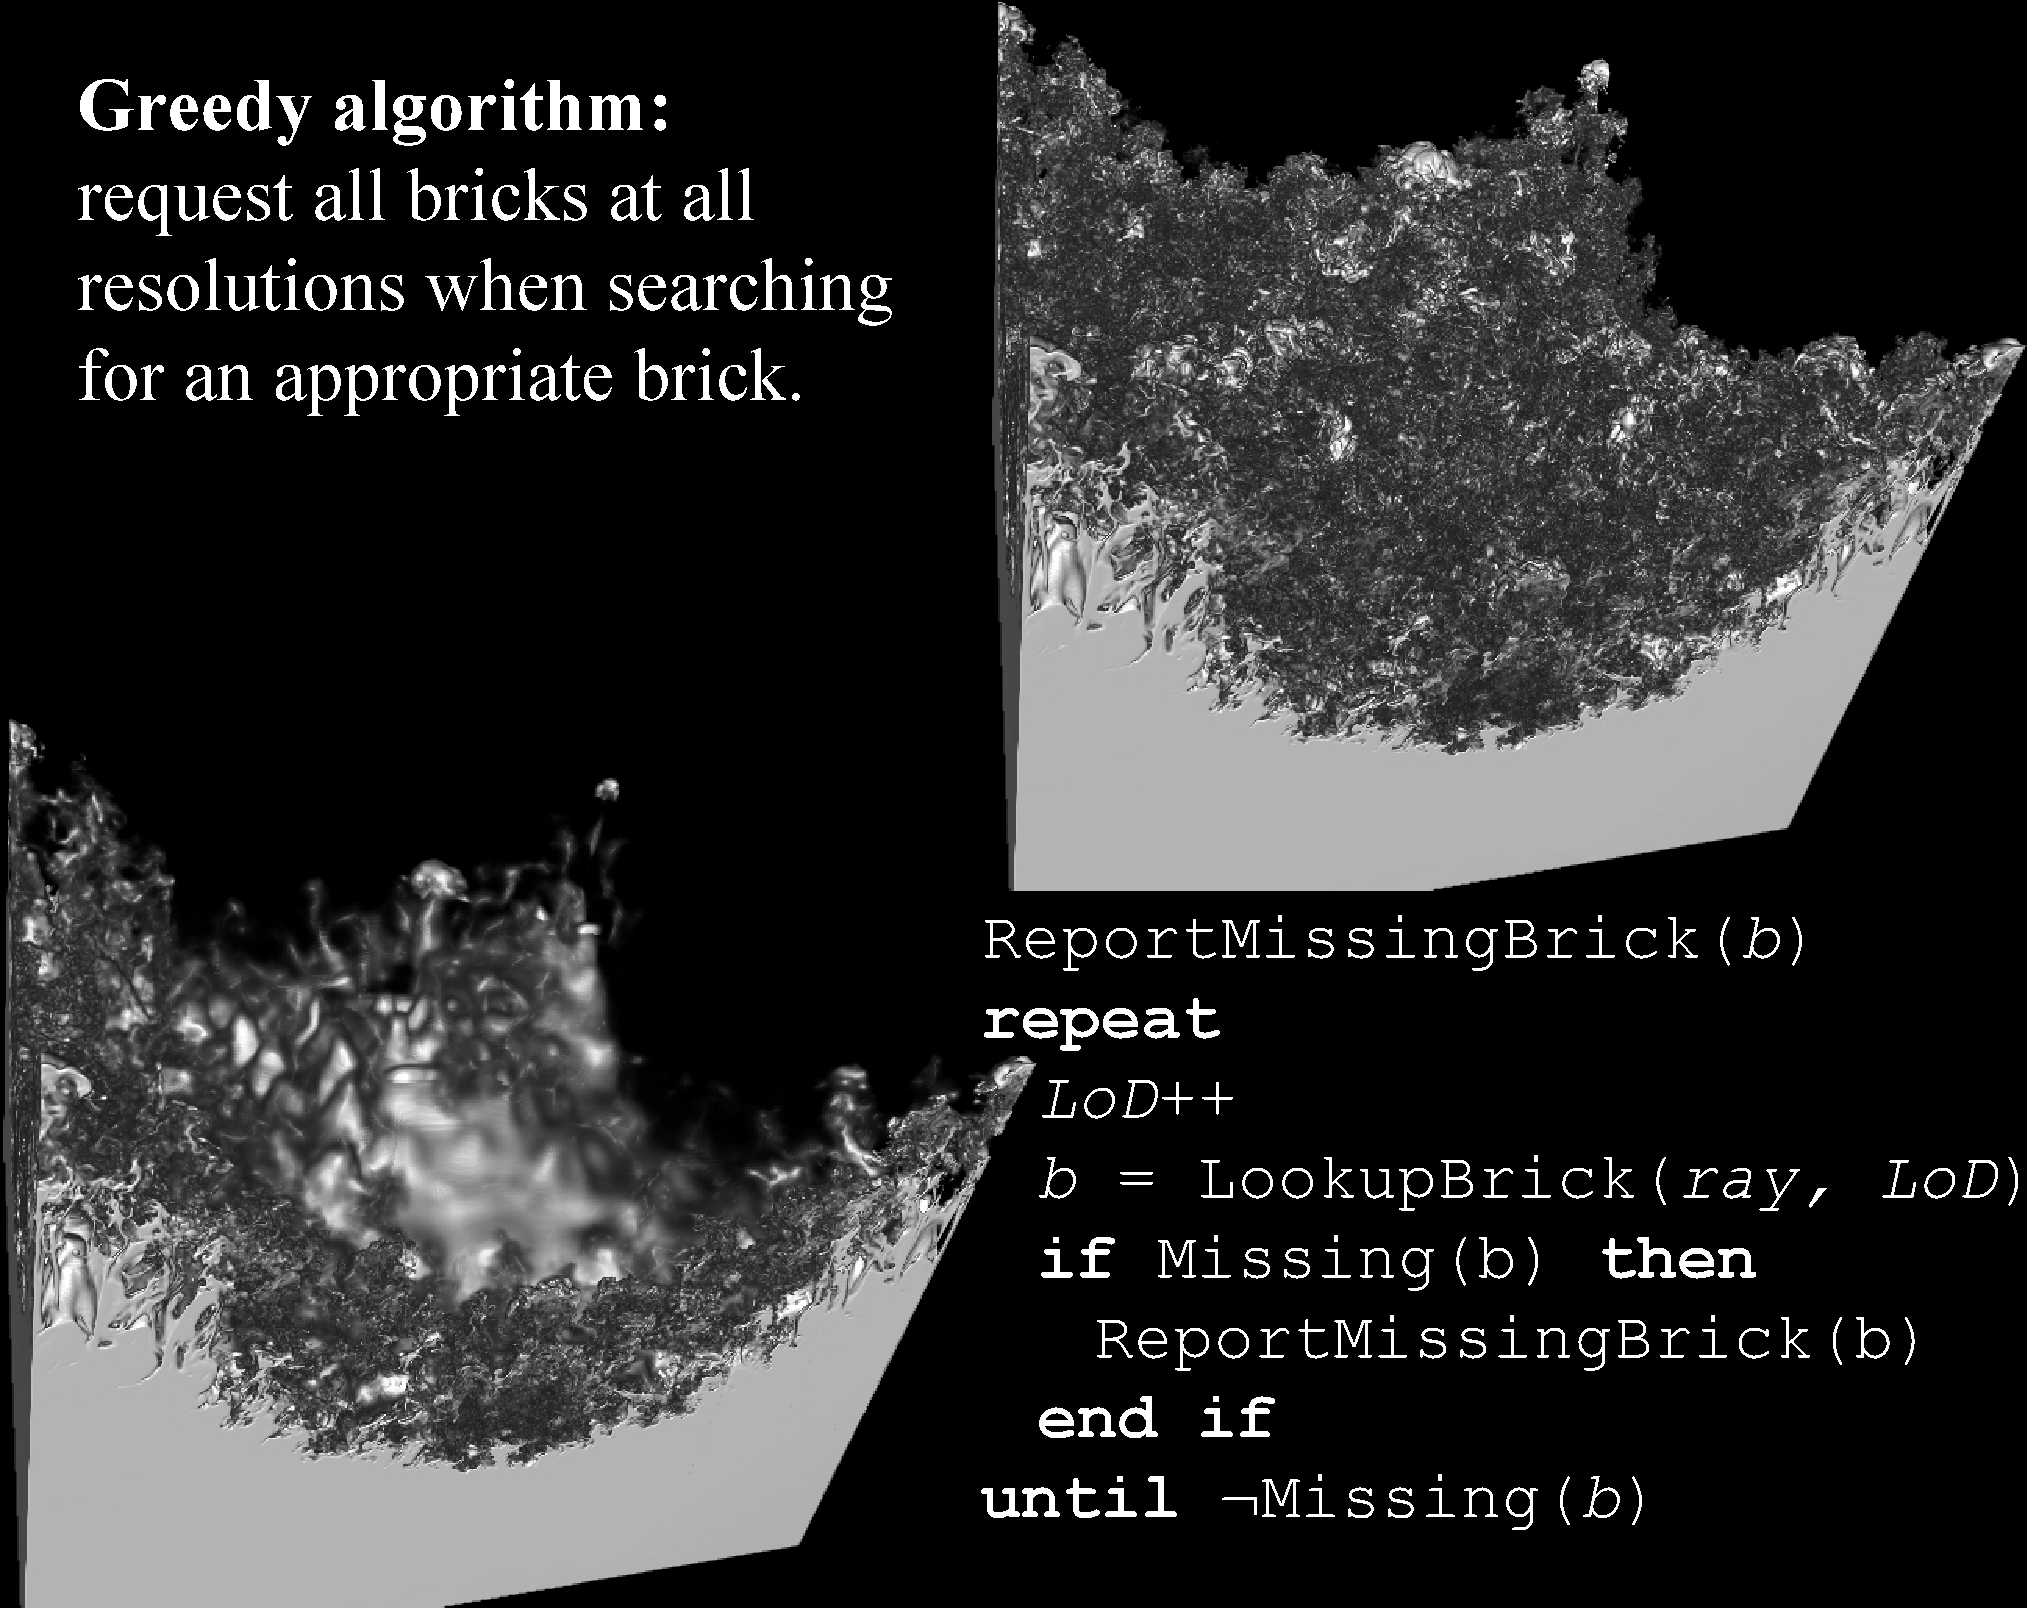
\includegraphics[width=0.99\linewidth]{images/Algorithm-Greedy}
  \caption{The effect of multiple brick replacement strategies.
  Renderings are select intermediate frames from the corresponding
  strategy.  `Greedy' strategies converge quicker and produce more
  densely-packed intermediate progress.}

  \label{figrg:strategy}
\end{figure*}

\subsection{CPU/GPU Interface}

Point (4) in our overview is the efficient communication of the ray
guidance information from the location it is generated---the GPU---to
the location it is utilized---the IO layer of a volume renderer.  This
section details how that communication happens.

We utilize a GPU-based hash table to store this data, though we note
that we really only require a set.  That is, our keys (brick IDs) are
our values, and we only care about their \emph{presence} in the table,
which we will read back and process as a list later.  A list would work
as well, but a hashing scheme allows concurrent inserts to proceed with
less contention.  During rendering, a ray may write into this table to
indicate that it
needs a non-resident brick to continue (see Figure \ref{figrg:flow},
(c)).  This small table will be read back from the GPU at the end of a
frame and utilized to fill the volume pool with new data.

As locks do not exist in current GLSL versions (and potentially never
will), lock-free structures are the only hazard-prone data structures
that can be correctly implemented.  Crassin et
al.\cite{Crassin:2009:Gigavoxels} workaround this by using multiple
render targets: each pixel has its own unique set of memory to
write into, and so there are no write hazards.  Our scheme requires
significantly less memory, but we must deal with these write hazards.

\subsubsection{Hash Table Parameters}
\label{sec:ht-params}

We map from the 4D index of the requested brick (spatial index + LoD)
to a unique 1D index in the hash table.  The mapping we utilize is
simply converting the 4D index into its equivalent 1D form, as if it
were stored in a 1D array.  We increment the index by 1 so that we may
use 0 to indicate that there is no entry at a location.

In a normal concurrent hash table, a lock is acquired for a table or
bucket before an access.  In lock-free data structures the primitives
used to implement locks are instead used directly on the data values
in question.  Inserts into our table proceed mostly as described in
previous
work~\cite{Michael:2002:LockFreeHT}.  In the face of concurrent
writes, this operation fails, and we attempt to probe a few times
(presently: 10) before giving up.

The critical piece to note is: \emph{it is not an error if a
missing brick is not recorded}.  As long as \emph{some}
missing bricks are recorded, the next frame \emph{will} make progress.
Each ray is either: finished, able to make progress, or unable to make
progress due to a lack of bricks that it requires.  Since our hash
table only contains entries for bricks that were requested by a ray,
then an invariant of our system is that: volume rendering is done, or
there exists at least one ray that can make progress.

% When a large number of bricks are needed, the hash table fills
% consistently, implying that collisions are infrequent or unimportant.
% If we vary the number of times rehashing is attempted from 5 to 100,
% for example, then performance differs by less than sampling noise,
% and the number of subframes decreases by barely 5\%, suggesting that
% collisions happen infrequently.

% Intuitively, the hash table size would have a large effect on
% performance.  Large tables should enable recording \emph{every}
% missing brick in a single pass, reducing the number of total passes
% required before convergence.  However, we found the size parameter
% to be negligible.  Regardless of how many rendering passes one does,
% the overall work is the same: the number of rendering passes will not
% change the number of bricks which must be loaded and rendered.  The
% only additional cost to an extra pass is the per-frame setup, which
% is independent of data size.
%
% One effect that small hash tables \emph{do} have is that they improve
% the response time of the renderer.  Since the next frame cannot begin
% until all bricks in the hash table are loaded, a small hash table
% creates a more iterative, progressive rendering experience.

\subsubsection{Strategies for Loading Coarser Bricks}

When the resolution required is missing during ray-casting, a ray's
brick requests can be what we call `greedy' or `global'.  In the
`greedy' case, the ray requests intermediate levels of detail along the
way, flooding the hash table with
requests that \textit{this} ray wants.  In the `global' case, each
ray only requests what it absolutely needs, leaving space for other
rays to request what they need.  These cases are visually depicted and
expounded in Figure
\ref{figrg:strategy}.

% \begin{figure}
%   \centering
%   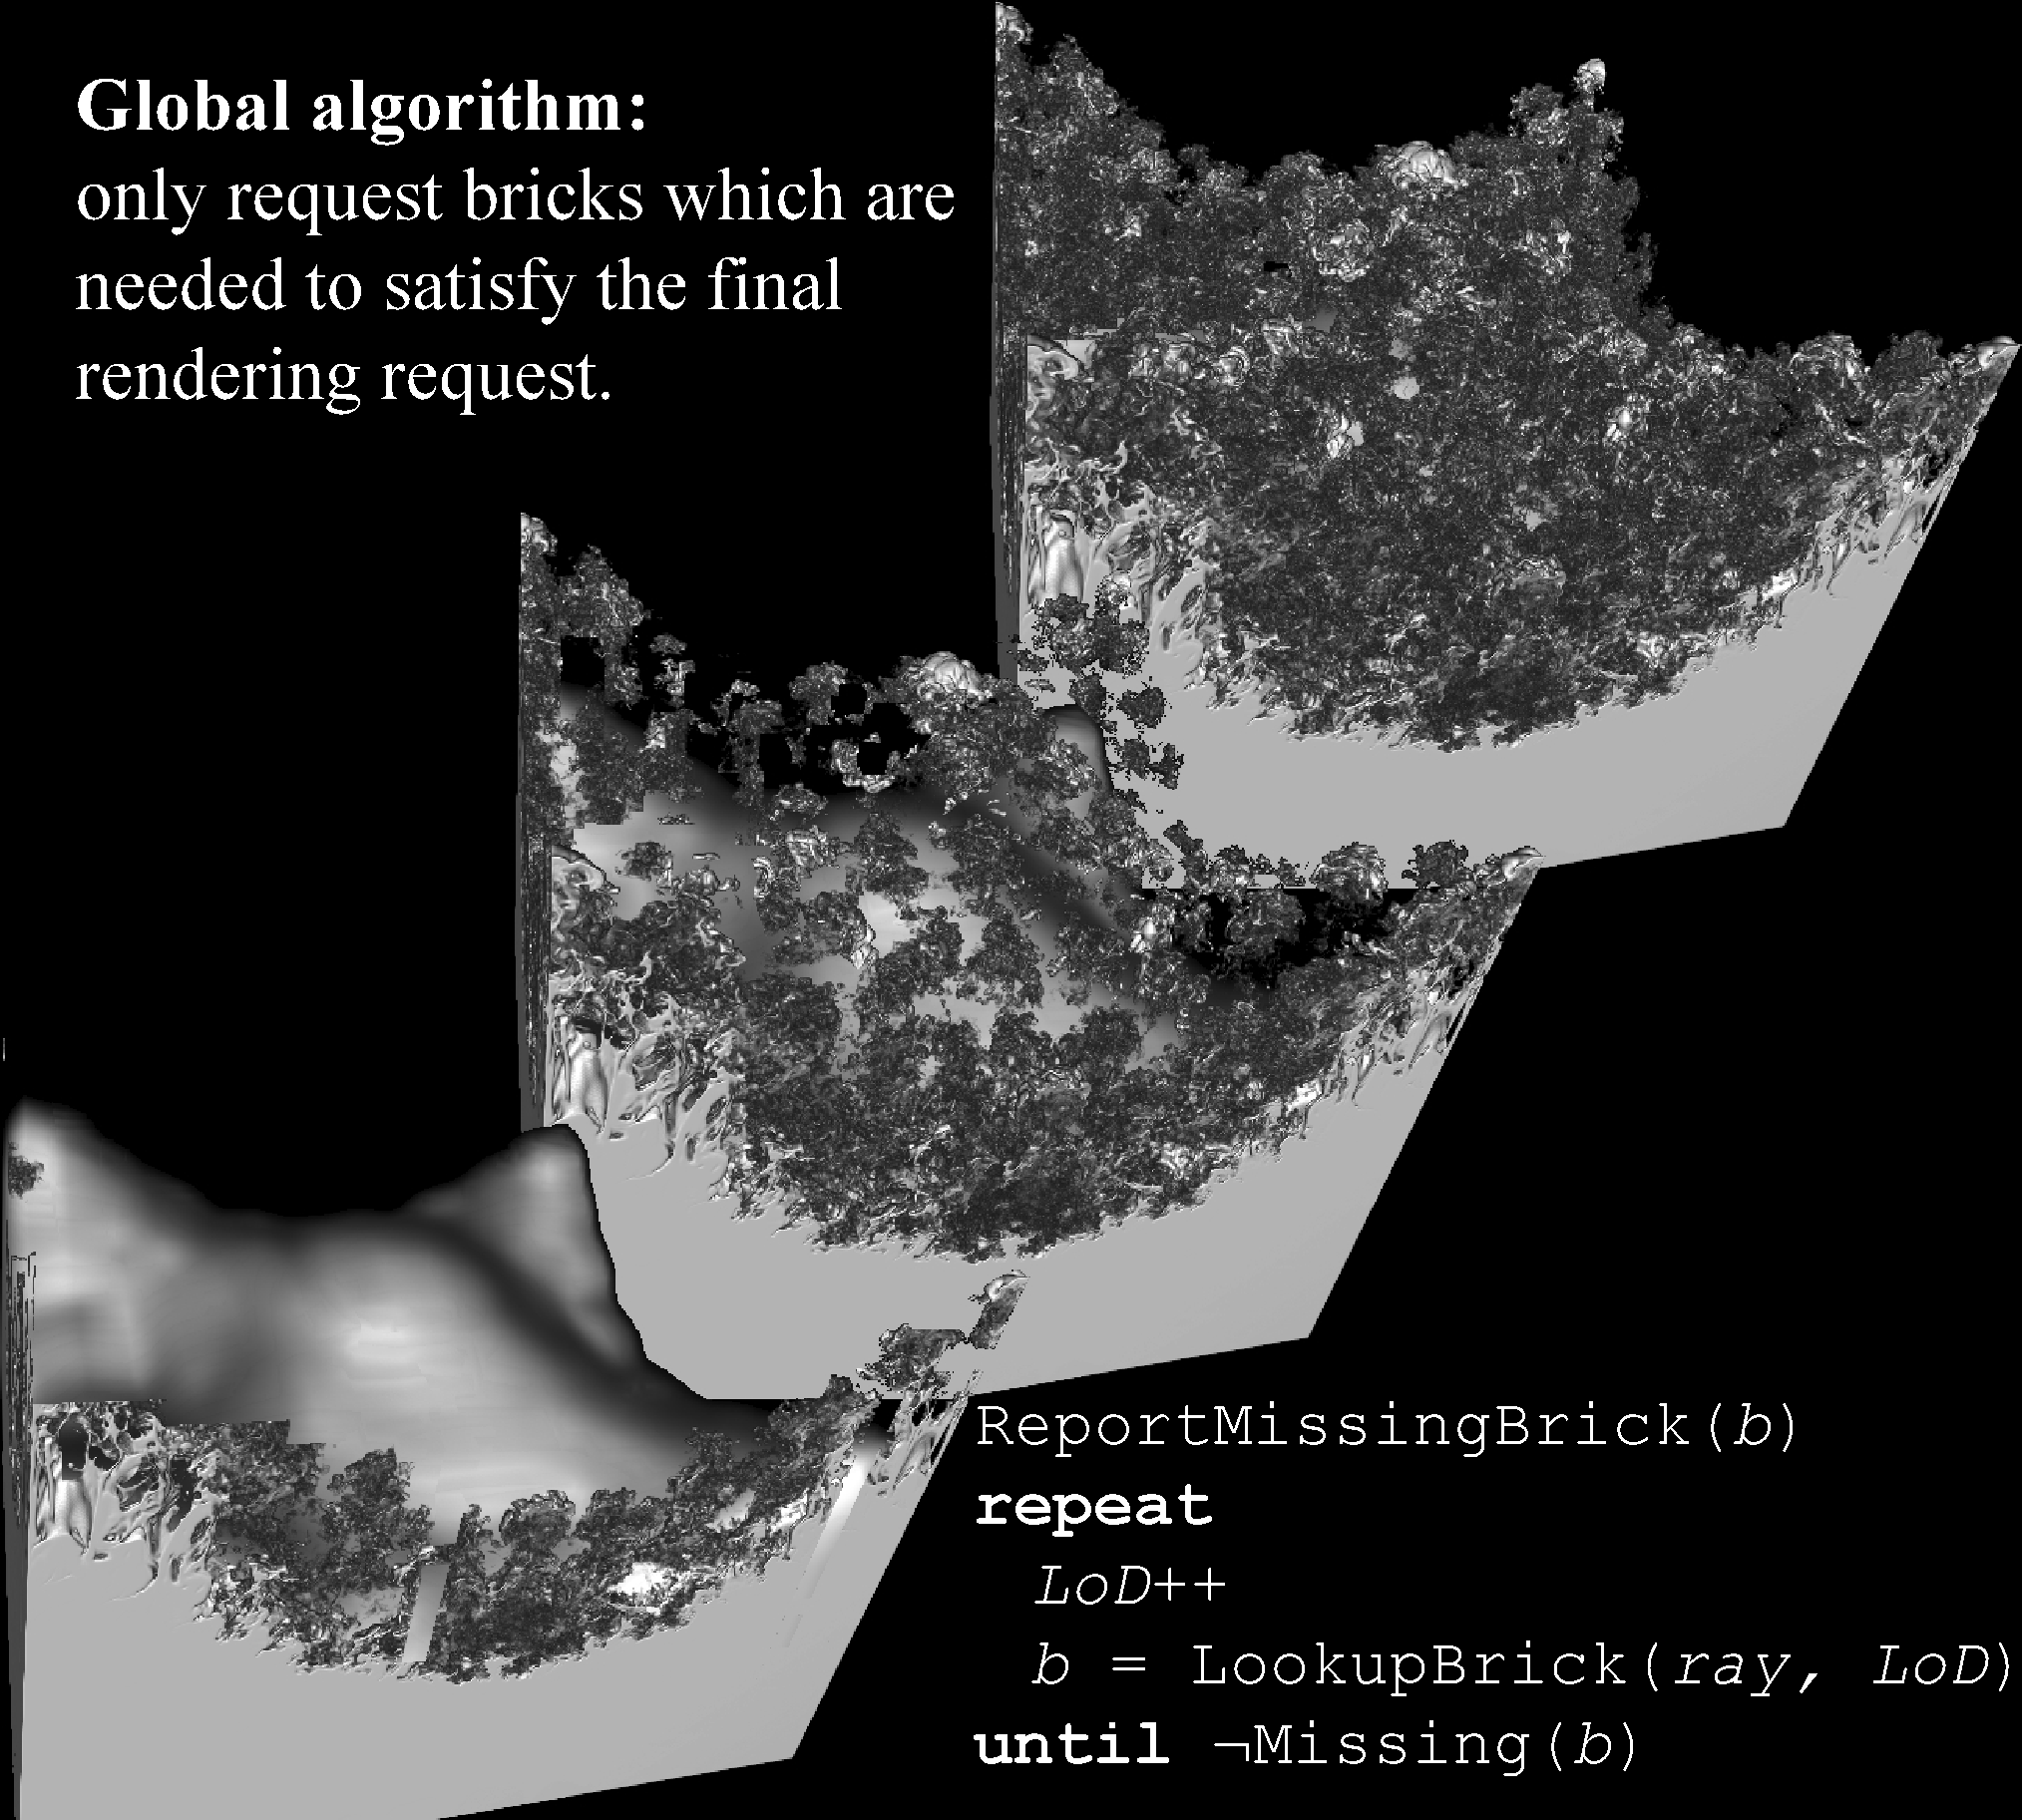
\includegraphics[width=0.99\linewidth]{images/Algorithm-Global}
%   \caption{The effect of multiple brick replacement strategies.
%   Renderings are select intermediate frames from the corresponding
%   strategy.  `Greedy' strategies converge quicker and produce more
%   densely-packed intermediate progress.}

%   \label{figrg:strategyGlobal}
% \end{figure}

% \begin{figure}
%   \centering
%   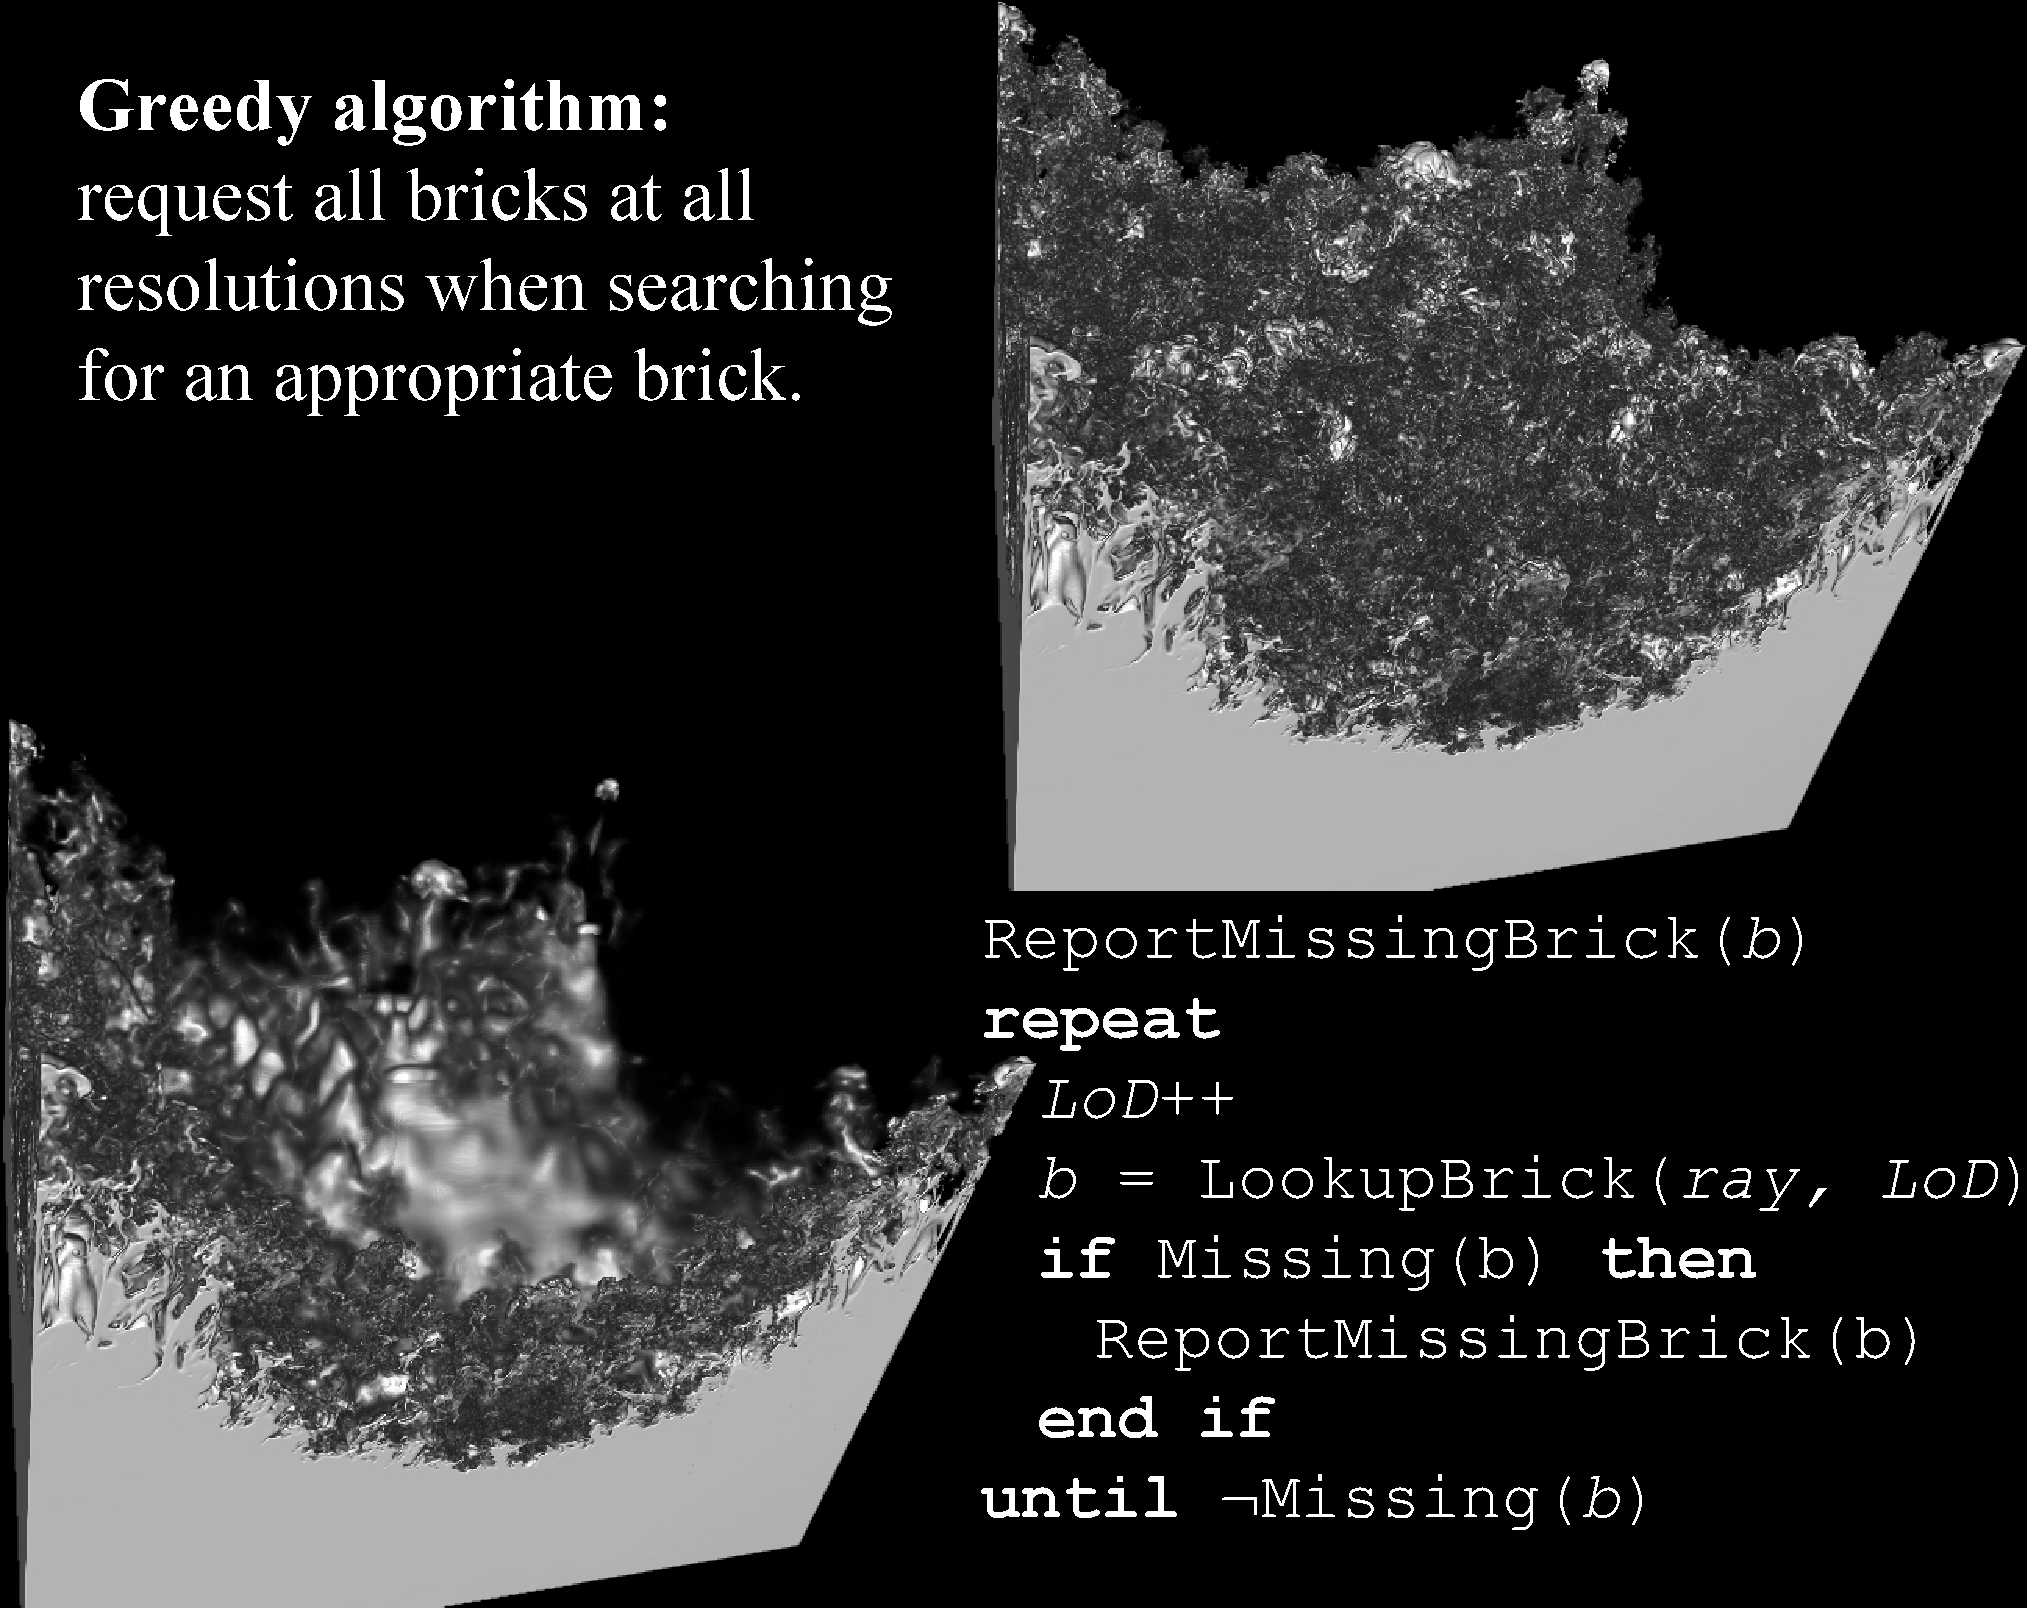
\includegraphics[width=0.99\linewidth]{images/Algorithm-Greedy}
%   \caption{The effect of multiple brick replacement strategies.
%   Renderings are select intermediate frames from the corresponding
%   strategy.  `Greedy' strategies converge quicker and produce more
%   densely-packed intermediate progress.}

%   \label{figrg:strategyGreedy}
% \end{figure}

The intuitive interpretation is that the `greedy' approach will produce
a more responsive, iteratively-refined image, whereas the `global'
approach will generate the final correct image quickest.  However, the
authors were surprised to find that the `greedy' approach both produces
more pleasing progress information \emph{and} converges in the fewest
number of frames.  This is because it allows a ray to sample at its
final resolution quickly, which can cause earlier ray termination.

\section{Conclusions, Limitations, \& Future Work}
\label{sec:conclusion}

In this work, we have introduced an efficient, out-of-core, ray guided
GPU volume renderer that scales to extremely large data.  The system
pulls inspiration from a patchwork of recent renderers, combining the
advantages of many and reimplementing some ideas in light of modern GPU
features.  We have also contributed an evaluation and discussion of the
tradeoffs inherent in the development of a modern ray-guided volume
renderer.

Based on the data here, we conclude that a ray-guided volume renderer
should work with bricks that are, on disk, $64^3$ or larger.  This
minimizes time spent doing IO (Figure~\ref{figrg:layout}), and makes
data layout irrelevant, obviating the need for a complicated component
of the code.  Since the required memory shrinks with the brick size,
generating $32^3$ or even $16^3$ bricks on-the-fly is desirable,
though exactly which size is unfortunately too data-specific to answer
generally.  While `bzlib' gives ideal compression ratios, it is very
slow to decompress, and therefore most implementations will want to
utilize `LZ4' compression.  A cache is a boon when data will not fit in
GPU memory but will fit in the host's memory.

We have made a best-effort attempt to design both favorable and
unfavorable conditions with which to test a volume renderer, but it
is possible some considerations have been omitted.  In particular,
this renderer and many others rely heavily on the assumption that
rays will saturate quickly.  Subjectively, we have found this to be
overwhelmingly valid for all our work in volume rendering, but this is
not a rule and has not been thoroughly evaluated.

A second issue is the rendering modes evaluated.  While our system
supports 2D transfer functions as well, all performance results
presented here utilized the 1D transfer function mode.  Advanced
rendering effects as well, such as those similar to ambient
occlusion~\cite{Schott:2009:DAOVR}, are omitted.  Such effects should
have a variable impact, positively correlating to the proportion of
rendering vs. IO times presented in
Figure~\ref{figrg:breakdown}.  Screen-space methods may provide
acceptable quality without (comparatively) impacting performance.

Finally, reformatting the data into a bricked hierarchy continues to
be the bane of high-performance volume rendering.  This result is not
expounded often enough in the literature.  We hope this paper helps
to reiterate to the community that the FLOPs may be free, but data
movement will kill performance.

Most importantly, we have contributed an evaluation and discussion
of the issues inherent in the development of a ray guided volume
renderer. As has been demonstrated, many of these choices are not as
clear as previous reports may have inadvertently implied.  The results
presented in this work clearly depict the tradeoffs, to aid system
designers in creating volume renderers that suit their particular
environment.

We hope to extend this work to more diverse visualization scenarios.
Ray-guidance-based isosurface generation is a natural candidate for
these ideas.  Furthermore, a common use case is combining an isosurface
with volume rendering, which has the potential to significantly change
such aspects as the working set size.  The general idea that rendering
should drive the visualization pipeline---as opposed to passively
consuming the output of earlier operations---is one that is applicable
in a much wider sense than that presented here.

%\appendix
\section{Data and Performance Details}
\label{sec:data}

\begin{figure}
  \centering
  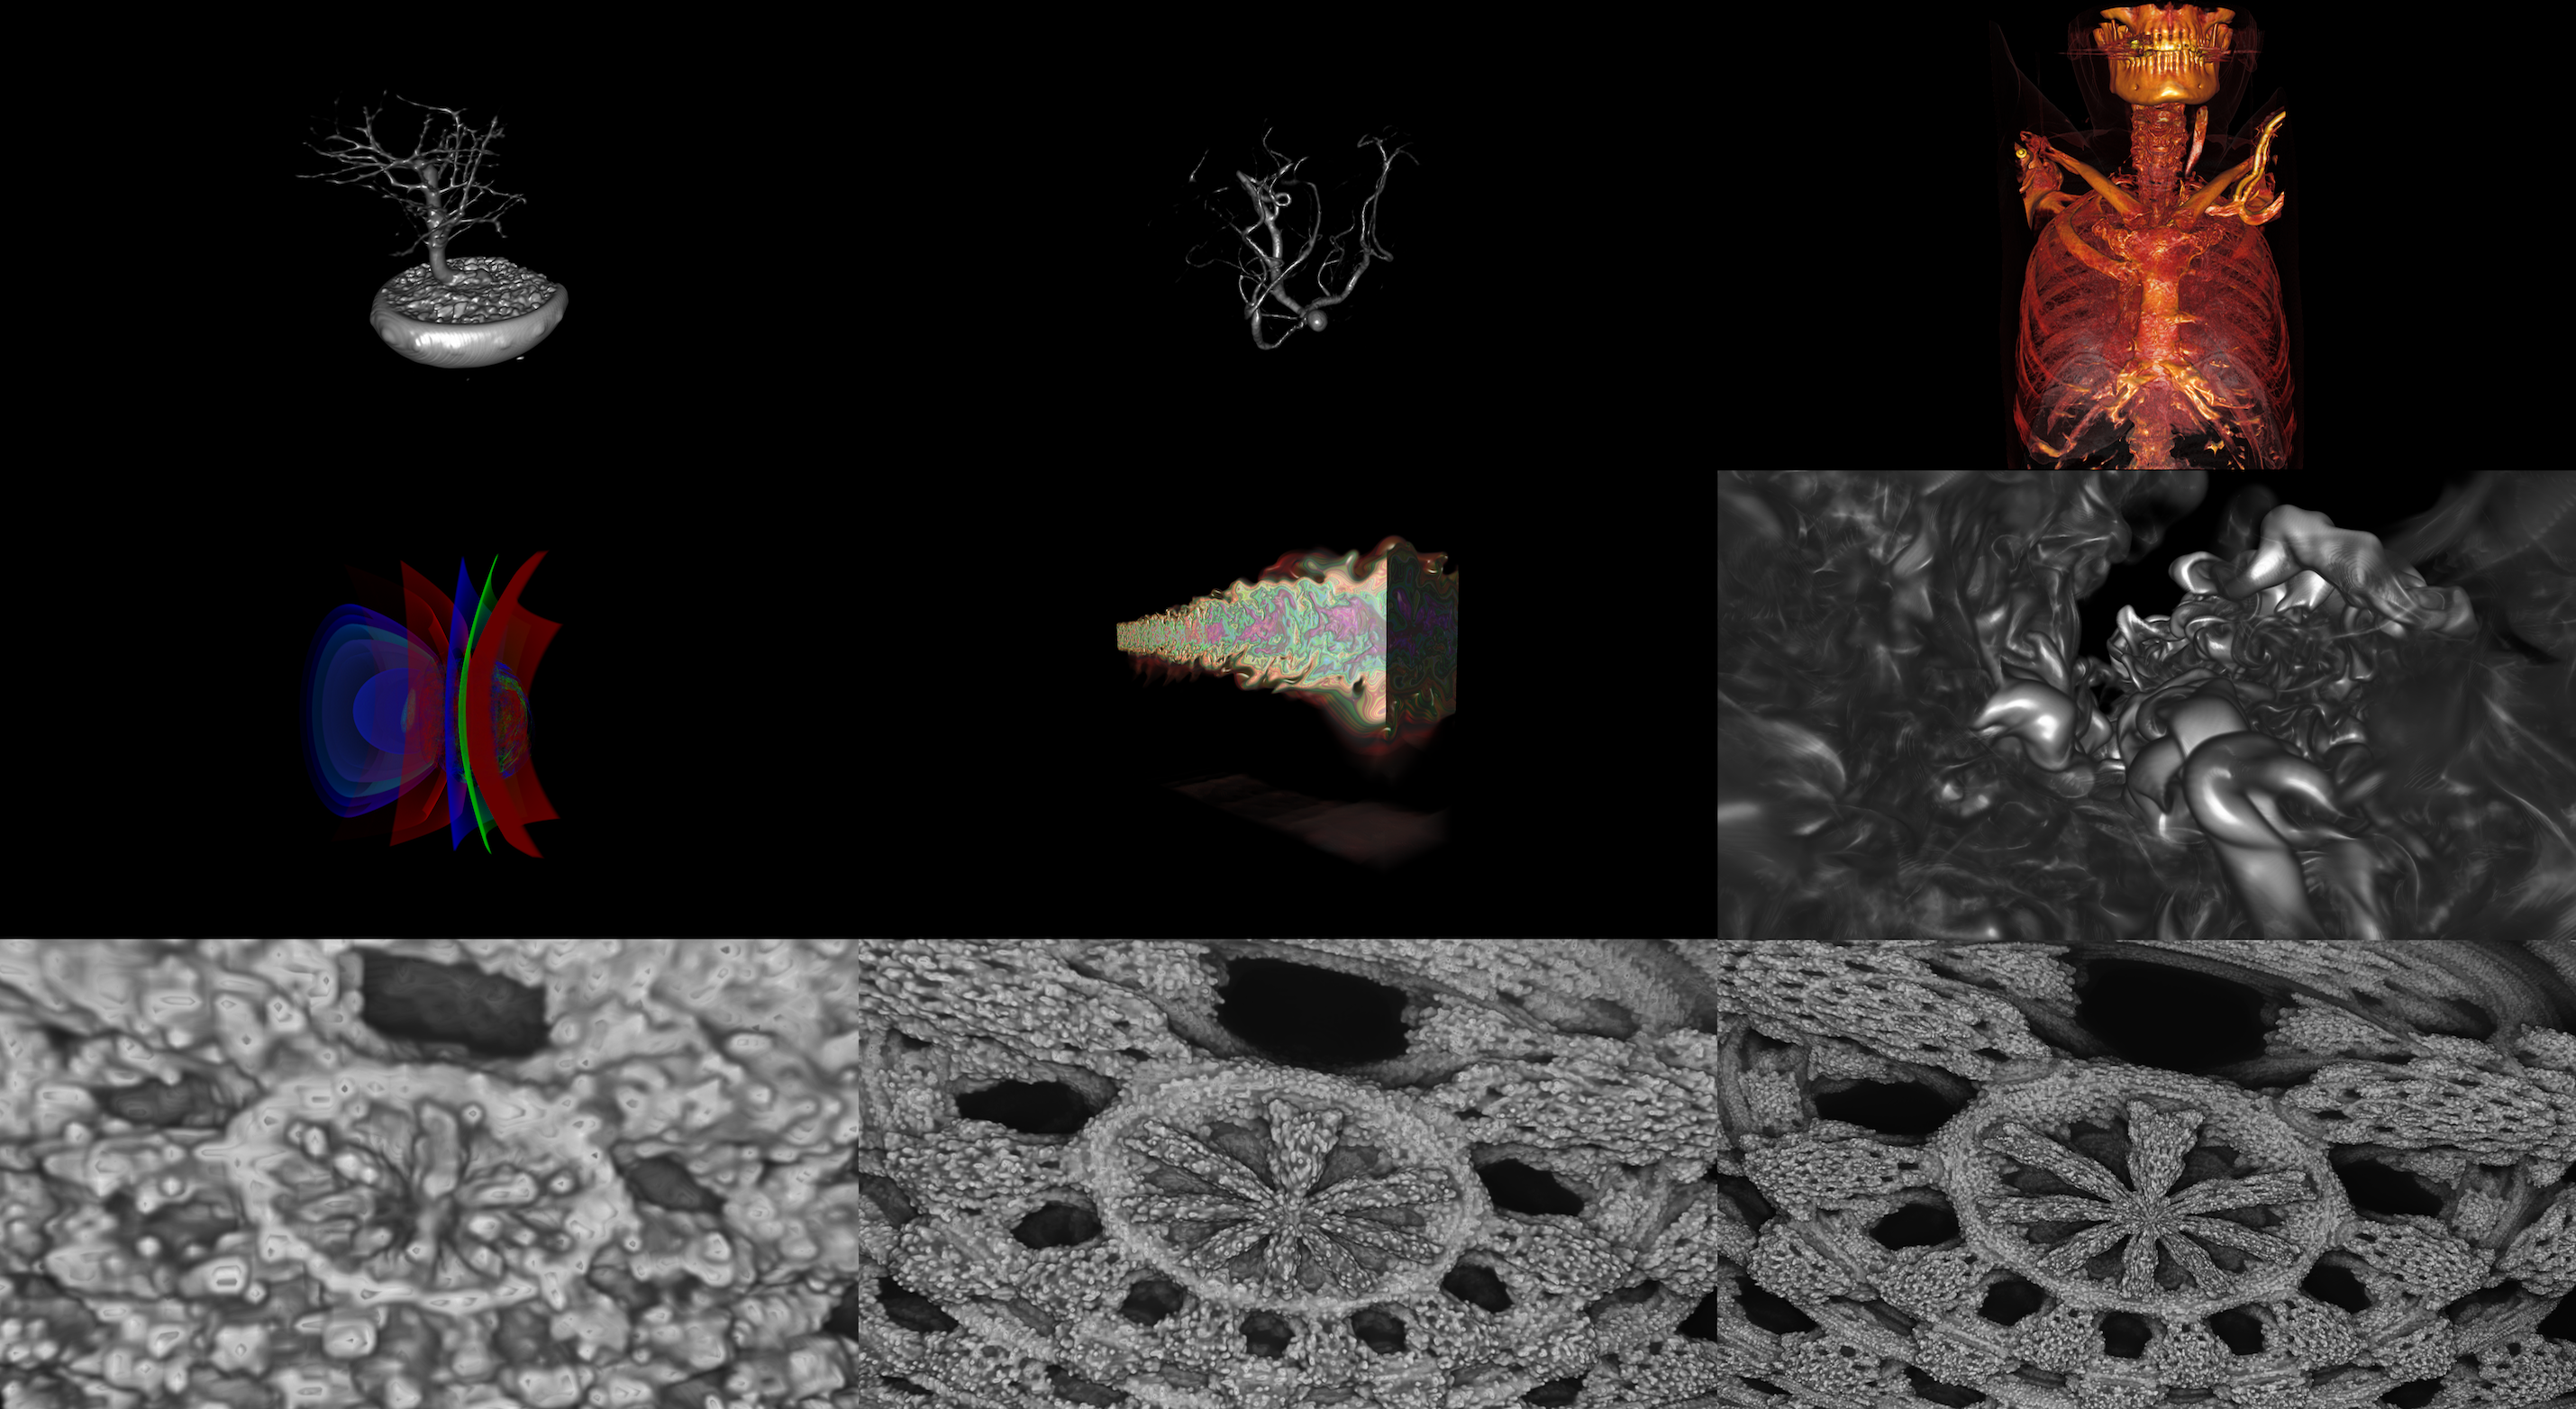
\includegraphics[width=0.98\linewidth]{images/rg/perFramesSmall.png}
  \caption{Selected frames from interactions used to record data for
  Table~\ref{tbl:timings} or Figure~\ref{figrg:breakdown}}
  \label{figrg:perFrames}
\end{figure}

We tested our renderer with a plethora of datasets, both real and
artificially created.  For space reasons, we discuss only a subset that
proved to be a reasonable sampling of our available data.
Renderer performance is depicted for a variety of datasets in
Table~\ref{tbl:timings}.  We discuss these in order of increasing size
here.

Two small datasets are the Bonsai tree (``Bonsai'') and ``Aneurysm''
datasets (Figure~\ref{figrg:perFrames}, top, left \& middle). While
small by today's standards, effective empty space leaping and early ray
termination still double the performance
(Table~\ref{tbl:timings}, note how performance doubles with smaller
brick sizes).

The ``WholeBody'' dataset (Figure~\ref{figrg:perFrames}, top, right) is
a contrast-enhanced CT scan of a human body.  As sometimes happens in
the biomedical domain, these data have limited slice resolution but a
plethora of slices.  Coarser resolutions must be careful to downsample
anisotropically, else the in-plane resolution washes out too quickly.

``Velocity'' (center, left) comes from the simulation of an exploding
star; we chose this dataset because our ideal transfer function for it
is quite transparent, preventing the renderer from taking advantage of
early ray termination.  Highly transparent transfer functions that
still produce informative results are a rarity but still occur.  For
these data, the additional overhead of small bricks can have a fairly
drastic effect on performance.  This dataset is one of the rare datasets
for that lighting actually makes the visualization \emph{more
difficult} to interpret, and so we always render this dataset with
lighting off.

The ``magnitude'' dataset (center, middle) comes from a combustion
simulation and represents another intermediate step towards larger
data.  The lower half of this dataset actually has a very faint trace
of data, which causes the renderer to sample densely.  The expense
of computing lighting information for fragments that ultimately
contribute very little has a notable effect on performance.

The Richtmyer-Meshkov Instability (``RMI'',
Figure~\ref{figrg:teaser} right and Figure~\ref{figrg:perFrames}, center,
right) and the Visible Human (Figure~\ref{figrg:teaser} left) are popular
datasets in the volume rendering literature; details can be found in
previous work.

We created a series of ``Mandelbulbs'' at various resolutions ($1k^3$,
$4k^3$, $8k^3$).  These are an extension of the mandelbrot fractal into
3 dimensions.  This has many of the same properties of the data used in
Crassin et al.~\cite{Crassin:2009:Gigavoxels}, in which Perlin noise
was added to a large bone scan to increase the sampling requirements.
We
create the high-resolution features \textit{a priori}, so no GPU
features were used to accelerate this process.  At equivalent
resolutions to that work, we see double to an order of magnitude
improved performance, but for this work we report results at 1080p HD
resolution.  A descriptive view of the Mandelbulb is
given in Figure~\ref{figrg:bricks-empty} and there
are close-ups visible in Figure~\ref{figrg:perFrames} (bottom row;
center, right).

\begin{table}
  \centering
  \caption{Per-frame rendering time at 6 different brick sizes, for
  a variety of datasets depicted in Figures~\ref{figrg:perFrames} and
  \ref{figrg:teaser}.  \textbf{Optimal brick sizes} are
  dataset dependent.}
  \label{tbl:timings}
  \rowcolors{4}{gray!20}{white}

  \begin{tabular*}{\linewidth}{|p{0.25825\linewidth}|p{0.11\linewidth}|p{0.11\linewidth}|p{0.11\linewidth}|p{0.11\linewidth}|p{0.11\linewidth}|}\hline
    & \multicolumn{5}{c|}{\textbf{Rendering Time (ms)}}\\
    \cline{2-6}
    \multicolumn{1}{|l|}{\textbf{Dataset}}
                  & $16^3$ & $32^3$ & $64^3$ & $128^3$ & $256^3$ \\\hline
    Bonsai        & {\bf 16} & 20     & 26         & 31  & 28        \\
    Head Aneurysm & {\bf 27} & 34     & 40         & 55  & 85        \\
    Whole Body    & 140      & 94     & 82         & 77  & {\bf 67}  \\
    Velocity      & 376      & 208    & 146        & 118 & {\bf 110} \\
    Magnitude     & 132      & 93     & {\bf 80}   & 82  & 85        \\
    RMI           & {\bf 60} & 64     & 61         & 67  & 67        \\
    Visible Human & {\bf 34} & 37     & 47         & 67  & 123       \\
    Mandelbulb1k  & {\bf 21} & {\bf 21} & {\bf 21} & 22  & 25        \\
    Mandelbulb4k  & {\bf 27} & 30     & 37         & 47  & 47        \\
    Mandelbulb8k  & {\bf 33} & 37     & 45         & 60  & 78        \\\hline
  \end{tabular*}
\end{table}

\begin{table}
  \centering
  \caption{Dataset properties for test datasets.}
  \label{tbl:sizes}
  % color breaks the r@{sep} stuff.  great! <3 TeX.
  %\rowcolors{2}{gray!20}{white}
  \begin{tabular*}{\linewidth}{|p{0.27\linewidth}|p{0.091\linewidth}@{$\times$}p{0.091\linewidth}@{$\times$}p{0.091\linewidth}p{0.105\linewidth}@{\quad}|p{0.16175\linewidth}|}\hline
    \multicolumn{1}{|l|}{\textbf{Dataset}} &
    \multicolumn{4}{c|}{\textbf{Resolution}} &
    \multicolumn{1}{c|}{\textbf{Size}}\\\hline
    Bonsai        & ~256 &$~256$ &$~256$ & 8 bpp  & 16 MB\\
    Head Aneurysm & ~512 &$~512$ &$~512$ & 16 bpp & 256 MB\\
    Whole Body    & ~512 &$~512$ &$3172$ & 16 bpp & 1.5 GB\\
    Velocity      & $1000$ &$1000$ &$1000$ & 16 bpp & 1.9 GB\\
    Magnitude     & $2025$ &$1600$ &$~400$ & 16 bpp & 2.4 GB\\
    RMI           & $2048$ &$2048$ &$1920$ & 8 bpp  & 7.5 GB\\
    Visible Human & $1728$ &$1008$ &$1878$ & 32 bpp & 12.2 GB\\
    Mandelbulb1k  & $1024$ &$1024$ &$1024$ & 8 bpp  & 1 GB\\
    Mandelbulb4k  & $4096$ &$4096$ &$4096$ & 8 bpp  & 64 GB\\
    Mandelbulb8k  & $8192$ &$8192$ &$8192$ & 8 bpp  & 512 GB\\\hline
  \end{tabular*}
\end{table}

\section{Source Code}

The renderer used in this work is freely available, as part of the
ImageVis3D~\cite{Fogal:2010:Tuvok} package.  We encourage others to
reproduce and build upon our results.


\chapter{Multi-scale parallel volume rendering}
\label{chp:multiscale}
\section{Abstract}

Data sets of immense size are regularly generated on large scale
computing resources.  Even among more traditional methods for
acquisition of volume data, such as MRI and CT scanners, data that is
too large to be effectively visualized on standard workstations is now
commonplace.

One solution to this problem is to employ a `visualization cluster,' a
small- to medium- scale cluster dedicated to performing visualization
and analysis of massive data sets generated on larger scale
supercomputers. These clusters are designed to fit a different
need than traditional supercomputers, and therefore their design
mandates different hardware choices, such as increased memory, and
more recently, graphics processing units (GPUs).  While there has
been much previous work on distributed memory visualization as well
as GPU visualization, there is a relative dearth of algorithms
that effectively use GPUs at a large scale in a distributed memory
environment.  In this work, we study a common visualization technique
in a GPU-accelerated, distributed memory setting, and present
performance charactersitcs when scaling to extremely large data sets.

\section{Introduction}
\label{sec:introduction}

Visualization and analysis algorithms, volume rendering in particular,
require extensive compute power relative to data set size.  One
possible solution is to use the large scale supercomputer that
generated the data, which clearly has the requisite compute power.
However it can be difficuilt to reserve and obtain the compute
resources required for viewing large data sets.  An alternative
approach, one explored in this work, is to use a smaller scale
cluster equipped with GPUs.  Such a cluster can provide the needed
computational power at a fraction of the cost---provided the GPUs
can be effectively utilized.  As a result, a semi-recent trend has
emerged to procure GPU-accelerated visualization clusters dedicated
to postprocessing the data generated by high-end supercomputers;
examples include ORNL's Lens, Argonne's Eureka, TACC's Longhorn, SCI's
Tesla-based cluster, and LLNL's Gauss.

Despite this trend, there have been relatively few efforts studying distributed
memory, GPU-accelerated visualization algorithms that can effectively utiliaze
the resources available on these clusters.  In this work, we report parallel
volume rendering performance characteristics on large data sets for a typ[ical
machine of this type.

Our system is divided into three stages:

\begin{enumerate}

  \item \emph{An intelligent pre-partitioning} that is designed to make
  combining results from different nodes easy.

  \item \emph{A GPU volume renderer} to perform per-frame volume
  rendering at interactive rates.

  \item \emph{MPI-based compositing} using a sort-last compositing framework.

\end{enumerate}

M\"uller et al. presented a system similar to our own that was limited
to smaller data sets~\cite{Needed}.  We have extended the ideas in that
system to allow for larger data sets, by removing the restriction that
a data set must fit in the combined texture memory of the GPU cluster
and adding the ability to mix in CPU-based renderers, enabling us to
analyze the parallel performance on extremely large data sets.  The
primary contribution of this component of our work is an increased
understanding of the performance characteristics of a distributed
memory GPU-accelerated volume rendering algorithm at a scale (256 GPUs)
much larger than previously published.  Further, the results presented
here (data sets up to $8192^3$ voxels) represent some of the largest
parallel volume renderings attempted thus far.

Our system and benchmarks allow us to explore issues such as:

\begin{itemize}

  \item the balance between rendering and compositing: a well-studied
  issue with CPU-based rendering, but currently with unclear
  performance tradeoffs for rendering on GPU clusters;

  \item the overhead of transferring data to and from a GPU;

  \item the importance of process-level load balancing; and

  \item the viability of GPU clusters for rendering very large data.

\end{itemize}

This chapter is organized as follows.  In Section~\ref{sec:previous},
we overview previous work in parallel compositing and GPU volume
rendering.  In Section~\ref{sec:arch}, we outline our system in detail.
Section~\ref{sec:eval} discusses our benchmarks and presents their
results. Finally, in Section~\ref{sec:conclusions} we draw conclusions
based on our findings.

\begin{figure}
  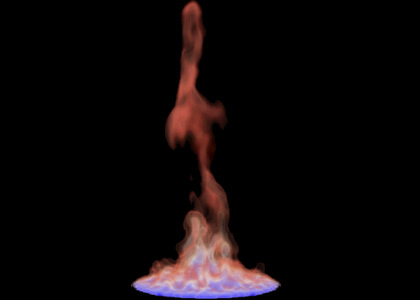
\includegraphics[width=\linewidth]{images/multiscale/teaser}
  \caption{Output of our volume rendering system with a data set
  representing a burning helium flame.}
  \label{fig:sample}
\end{figure}

\section{Previous work}
\label{sec:previous}

Volume rendering in a serial context has been studied for many years.
The
performance of the basic algorithm~\cite{Needed} was improved
significantly by incorporating empty space leaping and early ray
termination~\cite{Levoy:EarlyTermination}.  Max provided one of the
earliest formal presentations of the complete volume rendering equation
in~\cite{Needed}.  Despite significant algorithmic advances from
research such as~\cite{Levoy:EarlyTermination}, the largest increase in
performance for desktop volume renderers has come from taking advantage
of the 3D texture capabilities~\cite{Needed, Needed, Needed} and
programmable shaders~\cite{Krueger:2003:ATGV} available on modern
graphics hardware.

Extensive research has been done on parallel rendering and parallel
volume rendering.  Much of this work has focused on achieving
acceptable compositing times on large systems.  Molnar et al. conveyed
the theoretical underpinnings of rendering
performance~\cite{Molnar:199?:???}.  Earlier systems for parallel
volume rendering relied on direct send~\cite{Hsu:1993:???,
Ma:1993:???}, which divides the volume up into at least as many
chunks as there are processors, sending ray segments (fragments) to a
responsible tile node for compositing via the Porter and Duff
\emph{over} operator~\cite{PorterDuff:1984:Compositing}.  These
algorithms are simple to implement and integrate into existing systems,
but have sporadic compositing behavior and the potential to exchange a
large a number of fragments, straining the network layers when scaling
to large numbers of processors.  Tree-based compositing algorithms
feature more regular communication patterns, but impose an additional
latency that may not be required, depending on the particular frame
and data decomposition.  Binary swap and derivative algorithms are a
special case of tree-based algorithms that feature
equitable distribution of the compositing workload~\cite{Ma:1994:???}.
Despite advancements in compositing algorithms, network traffic remains
unevenly distributed in time, and thus high-performance networking
remains a necessity for subsecond rendering times on large numbers of
processors.

In the area of distributed memory parallel volume rendering of very
large data sets, the algorithm described by Ma et al
in~\cite{Ma:1993:???} has been taken to extreme scale in several
followuip publications.  In~\cite{Childs:2006:???}, data set sizes of
up to $3000^3$ are studied using hundreds of cores.  In this regime,
the time spent ray casting far exceeds the composite time.
In~\cite{PYRM:2008:???, PYR:2009:???}, the data set sizes range up to
$4480^3$, while core counts of tens of thousands are studied.
In~\cite{HBC:2010:???}, the benefits of hybrid parallelism are explored
at concurrency ranges going above two hundred thousand cores.  For both
of these studies, when going to extreme concurrency compositing time
becomes large and dominates ray-casting time.  This suggests that a
sweet spot may exist with GPU-accelerated distributed memory volume
rendering.  By using hardware acceleration, the long ray
casting times encountered in~\cite{Childs:2006:???} can be overcome.
Simultaneously, the emerging trend of composite-bound rendering
observed in~\cite{PYR:2009:???} and~\cite{HBC:2010:???} will be
mitigated by the ability to use many fewer nodes to command the same
compute power.

Numerous systems have been developed to enable parallel rendering in
existing software.  Among the most well-known is
Chromium~\cite{HHN:2002:???}, a rendering system that can transparently
parallelize OpenGL-based applications.  The Equalizer framework boasts
multiple compositing strategies, including an improved direct
send~\cite{EP:2007:???}.  The IceT library provides parallel rendering
with a variety of sort-last compositing strategies~\cite{MWP:2001:???}.

There has been less previous work studying volume rendering on
multiple GPUs.  Strengert et al. developed a system that used wavelet
compression and adaptively decompressed the data on small GPU
clusters~\cite{SMW:2004:???}.  Marchesin et al. compared a volume that
ran on two different two-GPU configurations: two GPUs on one system,
and one GPU on two networked systems~\cite{Marchesin:2008:MultiGPU}. The
use of just one or two systems, coupled with an in-core renderer,
artificially constrained the data set size.  M\"uller et al. developed
a distributed memory volume renderer that ran on
GPUs~\cite{Mueller:2006:???}; their system differs from ours in a few
key ways.  First, we use an out-of-core renderer and therefore can
exceed the available texture memory of the GPU by also utilizing CPU
memoryor disk.  To further reduce memory costs, we compute gradients
dynamically in the GLSL shader~\cite{KW:2003:???}, obviating the need
to upload a separate gradient texture.  This also has the benefit of
avoiding a pre-processing step, which is normally software-based in
existing general-purpose visualization applications (including the one
we chose to implement our system within) and can be time consuming for
large data sets.  Further differentiating our system and in line with
recent trends in visualization cluster architectures, we enable the use
of multiple GPUs per node.  M\"uller et al. used a direct send
compositing strategy~\cite{Hsu:1993:???, MPHK:1993:???}, whereas we use
a tree-based compositing method~\cite{MWP:2001:???}.  Finally, and
most importantly, we report performance results for substantially more
GPUs and much larger data sets, detailing the scalability of GPU-based
visualization clusters.  We therefore believe our work is the first
to evaluate the usability of distributed memory GPU clusters for this
scale of data.

\section{Architecture}
\label{sec:arch}

We implemented our remote rendering system inside of
VisIt~\cite{Childs:???:???}, which is capable of rendering data in
parallel on remote machines.  The system is comprised of a lightweight
`viewer' client application, connected over TCP to a server that
employs GPU cluster nodes.  All rendering is performed on the cluster,
composited via MPI, and images (optionally compressed via zlib) are
sent back to the viewer for display.  Example output from our system is
in Figure~\ref{fig:sample}.

Although VisIt provided a good starting point for our work, we needed
to make significant changes in order to implement our system.  In this
section, we highlight the main features of our system, taking special
care to note where we have deviated from existing VisIt functionality.

\subsection{Additions to VisIt}

\subsubsection{Multi-GPU access}

At the outset, VisIt's parallel server supported only a single GPU per
node.  We have revamped the manner in which VisIt accesses GPUs to
allow the system to take advantage of multi-GPU nodes.  When utilizing
GPU-based rendering, each GPU is matched to a CPU core that feeds
data to that GPU.  Additionally, when the number of CPU cores exceeds
the number of available GPUs, we allow for the use of software-based
renderers on the extra CPUs.  This code has been contributed to the
VisIt project.

\subsubsection{Partitioning}

VisIt contained a number of load decomposition stratgies prior to our
work.  However, we found these stratgies to be insufficient for a
variety of reasons:

\begin{enumerate}

  \item \textbf{Brick-based} Equalizing the distribution of work in
  VisIt was entirely based on \emph{bricks}, or pieces of the larger
  data set.  Our balancing algorithms use the time taken to render the
  previous frame to determine the weighted distribution of loads.

  \item \textbf{Master-slave} Dynamic balance algorithms in VisIt are
  based on a \emph{master} node that tells slaves to process a brick,
  waits for the slaves' completion, and then sends them a new brick to
  process.  We implemented a flat hierarchy, as seems to be more common
  in recent literature~\cite{Marchesin:2006:???, MSE06}.

  \item \textbf{Compositing} \emph{Most importantly}, for our
  object-based decomposition to work correctly, we needed a defined
  ordering to perform correct compositing.  The load balancing and
  compositing subsystems in VisIt were independent prior to our work.

\end{enumerate}

Our system relies on a \emph{k}d-tree for distributing and balancing
the data.  The spatial partitioning is done once initially and can
be adaptively refined by the rendering times from previous frames.
The initial tree only considers the number of bricks in the available
data set and attempts to distributed them evenly among processes, to
the extent that is possible.  When using static load balancing, this
decomposition is invariant for the life of the parallel job.
Figure~\ref{fig:decomposition} depicts a possible configuration
determined by the
partitioner, and shows the corresponding \emph{k}d-tree.

\begin{figure*}
  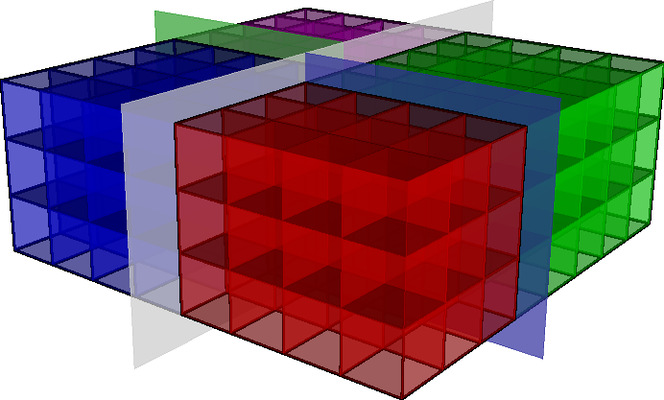
\includegraphics[width=0.49\linewidth]{images/multiscale/bricks.jpg}
  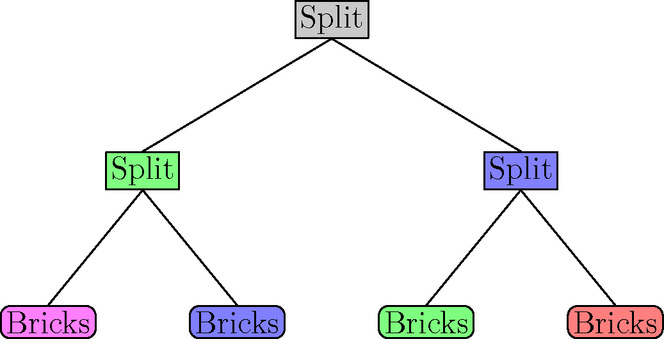
\includegraphics[width=0.49\linewidth]{images/multiscale/tree.jpg}
  \caption{Decomposition and corresponding kd-tree for an 8x8x3 grid
  of bricks divided among 4 processors.  Adjacent bricks are kept
  together for efficient rendering and compositing.  A composite order
  is derived dynamically from the camera location in relation to the
  splitting planes.  Note that the number of leaves in the tree is
  equal to the number of processes in the parallel rendering job.}
  \label{fig:decomposition}
\end{figure*}

When the dynamic load balancer is enabled, we use the last rendering
time on each process to determine the next configuration.  In our
initial implementation, the metric we utilized was the total pipeline
execution time to complete a frame.  This included the time to read
data from the disk, as well as the compositing time, among other
inputs.  However, we found that I/O would dwarf the actual rendering
time.  Further, compositing time is not dependent on the distribution
of bricks.  This therefore proved to be a poor metric.  Switching the
balancer to use the total render time for all bricks on that process
gave significantly better results.

In order to compare different implementations, we implemented multiple
load balancing algorithms, notably those described in Marchesin et al.
and M\"uller et al.'s work~\cite{Marchesin:2006:???, MSE06}.  In both cases, leaf
nodes represent processes, and each process has some number of bricks
assigned to it.  In the Marchesin-based approach, we start at the
parents of the leaf nodes and work our way up the tree, searching for
imbalance among siblings.  If two siblings are found to be imbalanced,
a single layer of bricks is moved along the splitting plane.  This
process continues up the root of the tree, at which time the virtual
results are committed and the new tree dictates the resulting data
distribution.  In the M\"uller-based approach, we begin with the root
node and use a pre-order traversal to find imbalance among siblings.
Once imbalance is found, the process stops for the current frame.
Instead of blindly shifting a layer of bricks between the siblings,
the method derives the average rendering cost associated with a layer
of bricks along the split plane, and shifts this layer if the new
configuration is projected to improve rendering time.

In addition to achieving a relatively even balance among the data, the
\emph{k}d-tree is used in the final stages to derive a valid sort-last
compositing order.

\section{Evaluation}
\label{sec:eval}

We implemented and tested our system on \textit{Lens}, a GPU-accelerated
visualization cluster housed at ORNL.  However, we were only able to access 16
GPUs on that machine.  In order to access a larger number of GPUs, we
transitioned to \textit{Longhorn}, a larger cluster housed at the Texas
Advanced Computing Cluster (TACC).  Specifications for each cluster are listed
in Table~\ref{tbl:clusters}.  Due to machine availability and configuration, we
were not able to fully utilize either machine.

\subsection{Rendering times}

The two dominant factors in distributed memory visualization
performance are the time taken to render the data and the time taken
to composite the resulting sub-images.  These have the largest impact
on usability because they comprise the majority of the latency a user
experiences: the time between when the user interacts with the data and
when the result of that interaction are displayed.

\begin{figure}
  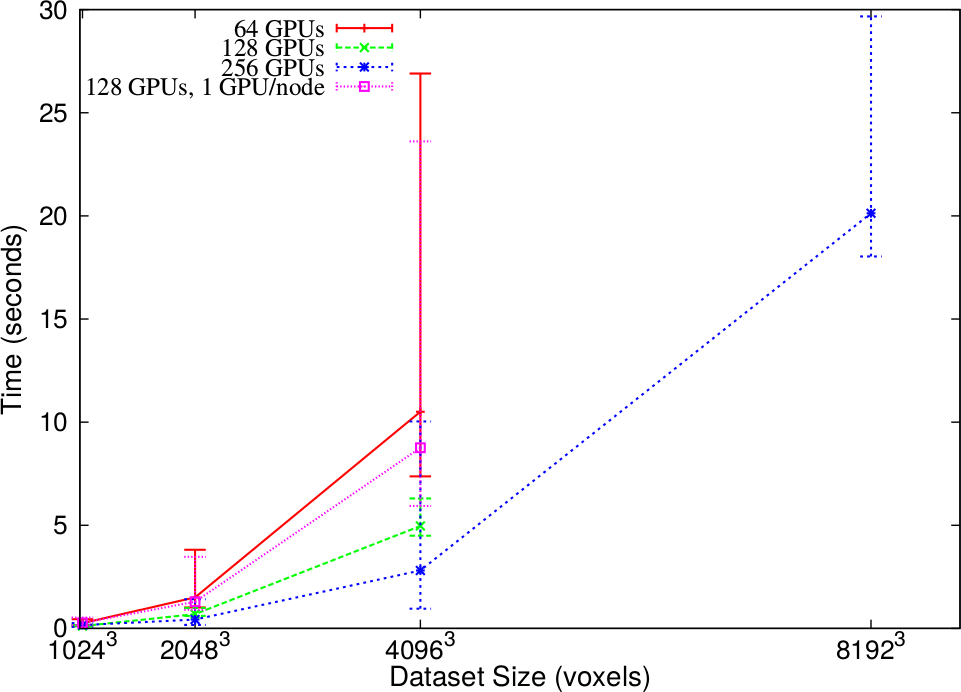
\includegraphics[width=\linewidth]{images/multiscale/rtime}

  \caption{Overal rendering time when rendering to a 1024x768 viewport
  on Longhorn.  This incorporates both rendering and compositing, and
  therefore shows the delay a user would experience if they used the
  system on a local network. Data points are the average across many
  frames, and error bars indicate the rendering timesor the slwoest and
  quickest frames, respectively.  For these results we used a domain
  consisteing of $13^3$ bricks (varying brick size) with the exceptions
  that all runs in the 128 GPU cases used $8^3$ bricks, and the run for
  the $8192^3$ data set was done using $32^3$ bricks.}
  \label{fig:rtime}
\end{figure}

Our data originated from a simulation performed by the Center for Simulation of
Accidental Fires and Exploisions (C-SAFE), desinged to study the instabilities
in a burning helum flame.  In order to study performance at varying
resolutions, we resampled this data to $1024^3$, $2048^3$, $4096^3$, and
$8192^3$, at a variety of bricks sizes.  We then performed tests, varying data
resolution, image resolution, choice of brick size, and number of GPUs, up to
256.  Unless noted otherwise, we divided the data into a grid of $8x8x8$ bricks
for parallel processing (larger data sets used larger bricks), and rendered
into a 1024x768 viewport.

Figure~\ref{fig:rtime} shows the scalability on the \textit{Longhorn}
cluster.  The principal input that affects rendering time is the data
set size, as one might expect.  These runs were all done using 2 GPUs
per node, except the ``128 GPUs, 1 GPU/node'' case, which was run on
128 nodes, each accessing a single GPU.  With very large data, there is
a modest increase in performance for this experimental setup.

\begin{figure}
  %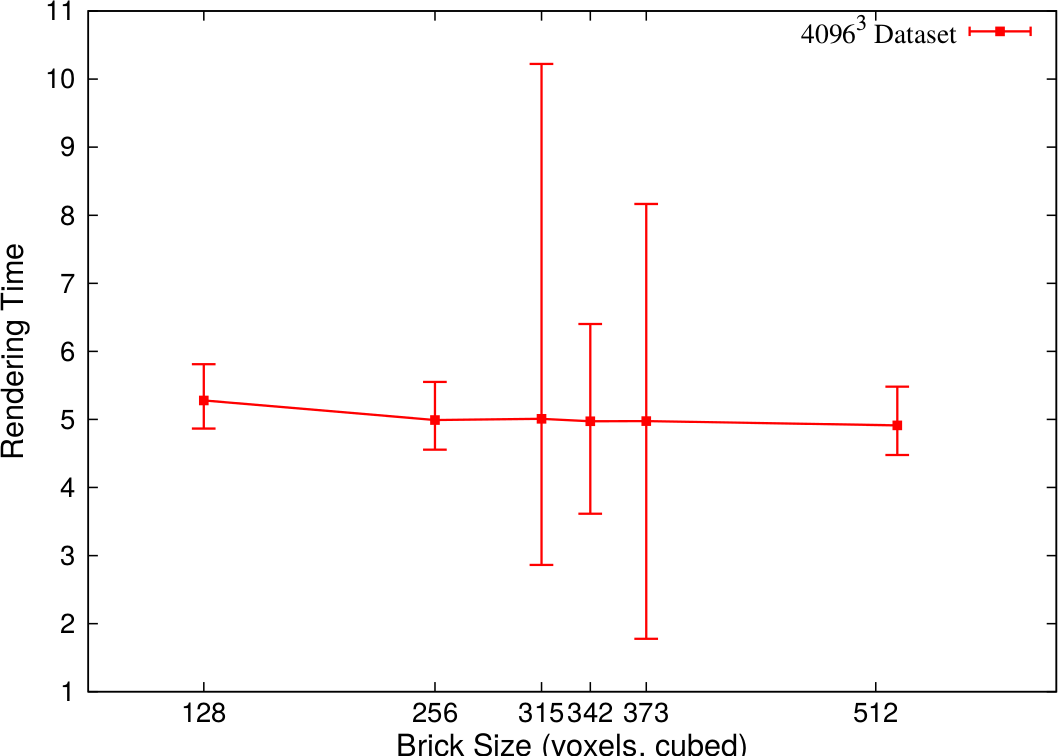
\includegraphics[width=\linewidth]{images/multiscale/bsize}

  \caption{Rendering time as a function of brick size.  Error bars
  indicate the minimum and maximum times recorded, across all nodes,
  for that particular brick size; high diswparity indicates the
  rendering time per-brick was highly variable, and load imbalance
  was therefore likely.  All tests were done with a $4096^3$ data
  set statically laod balanced across 128 GPUs on 64 nodes, using a
  scripted camera that requested the same viewpoints each run.  Note
  that the choice of brick size matters little in the average case, but
  bricks using non-power-of-two sizes give widely varying performance.
  Though raw data shows it is only hundreths of a second faster than
  $256^3$.}
  \label{fig:bsize}
\end{figure}

As can be seen in Figure~\ref{fig:bsize}, the brick size
\emph{generally} has little impact on performance.  A parallel volume
renderer's performance is, however, dictated by the slowest component,
and therefore the average rendering time is less important than the
maximum rendering time.  Taking that into account, it is clear that
brick sizes that are not a power of two are poor choices.  Dropping
down to $128^3$, we can see that per-brick overhead begins to become
noticeable, impacting overall rendering times.  We found larger bricks
sizes of $512^3$ give the absolute best performance, with $256^3$ a
good choice as well, as the differences are minor enough that they may
almost be considered sampling error.  Of course, such recommendations
may be specific to the GPUs
used in \textit{Longhorn}

We were initially surprised to find that the image resolution, while
relevant, was not a significant factor in the overall rendering
time.  When developing single GPU applications that run on a user's
desktop, our experience was the opposite: that image size does play a
significant role in performance.  We at first thought this was due to
skipping bricks that were `empty' under our transfer function---our
domain is perfectly cubic, yet as is displayed in
Figure~\ref{fig:sample} very little of the domain is actually
visible---but even after changing to a transfer function with no ``0''
values in the opacity map, rendering times changed very little.  We
concluded that the data sizes are so large compared to the number of
pixels rendered that the image size is dwarfed by comparison.

In our initial implementaion on \textit{Lens}, we noticed that we
began to strain the memory allocators while rendering a $3000^3$ data
set, as we approached low memory conditions.  Our volume renderer
automatically accounts for low memory conditions and attempts to free
unused bricks before failing outright.  However, an operating system
will thrash excessively before finally deciding to fail an allocation,
and therefore during the time leading up to a failed allocation,
performance will drop considerably.  Worse, we are working in a large
existing code base, and attempting to manage allocations outside our
own subsystems would prove unwieldy.  As such, we found the original
scheme to be unstable; the rendering system would create memory
pressure, causing other subsystems to fail an allocation in areas where
it may be difficult or impossible to ask our volume renderer to free up
memory.

To solve this problem, we render the data in a true out-of-core
fashion: bricks are given to the renderer, rendered into a framebuffer object,
and immediately thrown away.  One might expect that out-of-core algorithms would
have more per-block overhead and therefore be slower than an in-core algorithm.
As shown in Figure~\ref{fig:ooc}, the out-of-core approach actually
outperforms the analogous in-core approach even when there is
sufficient memory to hold the data set at once.  The reasoning
turned out to be that bricks were searched for in a logarithmic data
structure; the conservative approach taken by the out-of-core algorithm
meant that the container maxed out at a single element, accounting for
a minor performance improvement.

\begin{figure}
  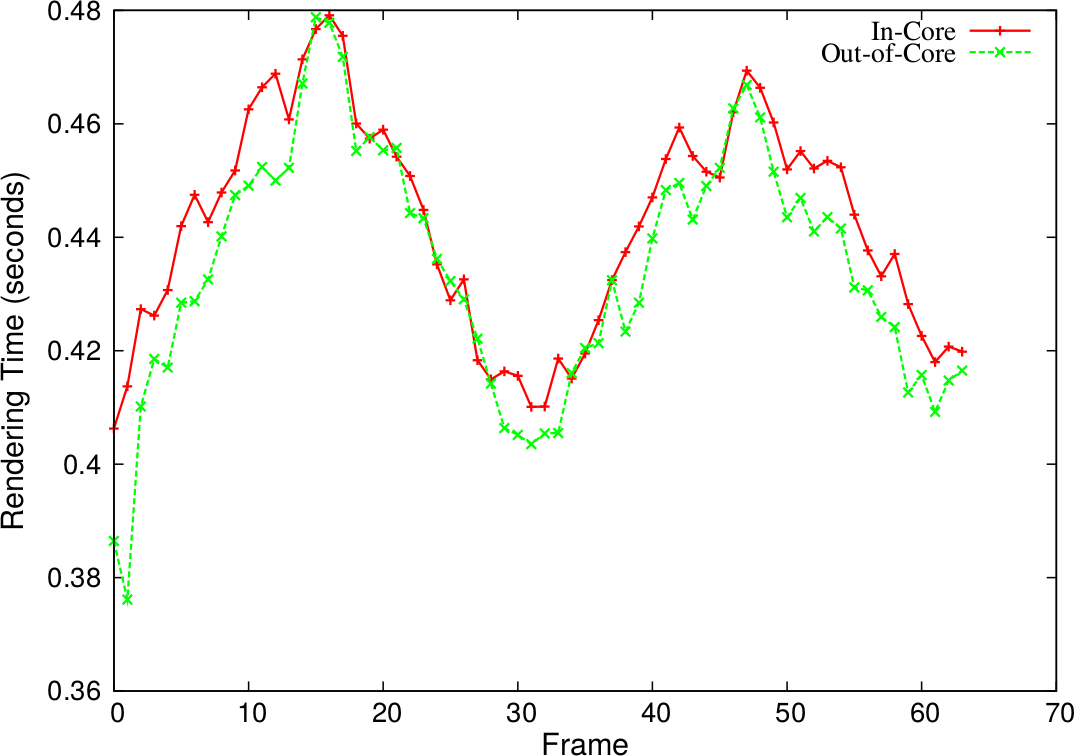
\includegraphics[width=\linewidth]{images/multiscale/ooc}
  \caption{Rendering times, per frame, for the in-core and out-of-core
  approaches to rendering a $1024^3$ data set (which fits comfortably
  in memory) across $16$ GPUs.  Additional processing in the
  out-of-core case doeds not negatively impact performance.}
  \label{fig:ooc}
\end{figure}

\subsubsection{Readback and compositing}

In earlier results, particularly with GPU-based rendering
architectures, the community was generally concerned with the time
required to read the resulting image data from the GPU and into the
host's
memory~\cite{Marchesin:2008:MultiGPU}.  Our study did not provide
corroboration of this concern, which we interpret as a positive data
point with respect to evolving graphics subsystems.  Our system did
demonstrate that this time increased as the resolution grew, but as can
be seen
in Table~\ref{tbl:breakdown}, even at 1024x768 this step took only
thousandths of a second.

\begin{table}
	\begin{tabular}{|c|ccc|c|}\hline
	\textbf{Dataset size} & \textbf{Rendering (s)} & \textbf{Readback (s)} &
		\textbf{Compositing (s)} & \textbf{Total (s)}\\\hline
	$1024^3$ &  0.06141 & 0.00328 & 0.06141 &  0.12610 \\
	$2048^3$ &  0.35107 & 0.00377 & 0.07673 &  0.43157 \\
	$4096^3$ &  2.50984 & 0.00377 & 0.29533 &  2.80894 \\
	$8192^3$ & 19.60648 & 0.00373 & 0.51799 & 20.12820 \\\hline
	\end{tabular}

  \caption{Breakdown of different pipeline stages for various data set
  sizes on 256 GPUs rendering into a $1024 \times 768$ viewport.  All
  times are in seconds.  The $1024^3$, $2048^3$, and $4096^3$ case used
  $13^3$ bricks (varying brick size); the $8192^3$ case used $32^3$
  bricks, making each brick $256^3$ voxels.  Compositing time rises
  only artificially; if a node finishes rendering before other nodes,
  the time it must wait was included under `Compositing' due to an
  artifact of our sampling code.  Thus, the data imply that larger data
  sets see more load imbalance.}

	\label{tbl:breakdown}
\end{table}

The time required for image composition is significantly reduced when
taking advantage of the GPUs available in the visualization vluster.
Since a GPU can render much faster than a software-based renderer, one
can achieve acceptable rendering performance using far fewer nodes.
Compositing, as it scales with the number of nodes involved in the
compositing process, improves significantly by utilizing many fewer
nodes.

\subsection{Load balancing}

We also sought to examine the utility of load balancing algorithms for
our system. We have implemented the algorithms as presented in two
recent parallel volume rendering papers, and compared rendering times
to each other and to a
statically balanced case.  Figure~\ref{fig:balance} illustrates
the comparisons, where the times shown are the maximum across all
processes.

\begin{figure}
  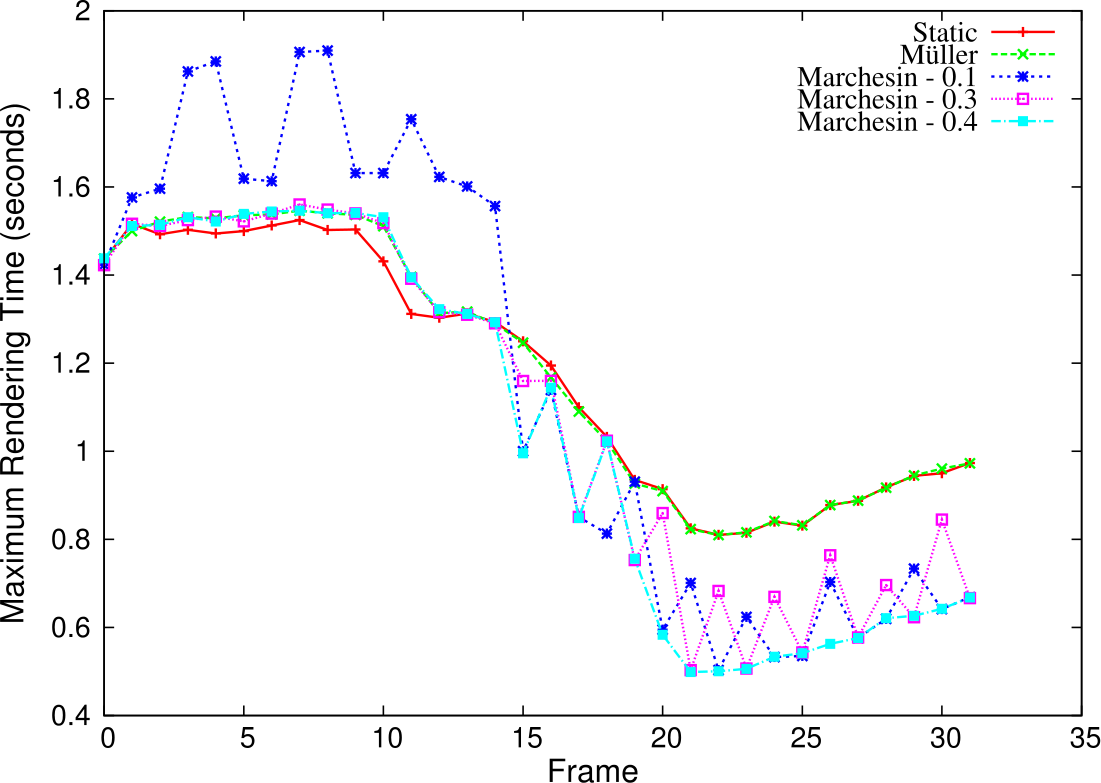
\includegraphics[width=\linewidth]{images/multiscale/balance}
  \caption{The maximum rendering time across all nodes under various
  load balancing algorithms.  The numbers after the `Marchesin'
  algorithms indicate thresholds: rendering disparity under these
  thresholds is ignored.}
  \label{fig:balance}
\end{figure}

We did a variety of experiments with multiple load balancer
implementations, using 8 or 16 GPUs.  Our initiali flythrough dequence
proved to be inappropriate for the application of a load balancer, as
there was not enough imbalance in the system to observe a significant
benefit.  We then attempted to
a `zoom out' flythrough, but rendering times decreasing on \emph{all}
nodes was not a case the the balancers we implemented could effectively
deal with: we found many cases where the balancers would shift data
to a node that was previously idle or at least doing very little
work, and a frame or two later the workload on such nodes would
spike.  This occurred because these nodes had both 1) received new
data as part of the balance and, 2) retained old data as part of the
initial decomposition or previous balancing processes.  The sudden
additional workload of previously invisible bricks caused these nodes
to overcompensate, sending data to other ``idle'' nodes---nodes that
would experience the sample problem in subsequent frames.

In previous work, authors have praised the effect load balancing has
when
zooming \emph{in} to a data set.  This naturally creates imbalance, as
some nodes end up with data that are not rendered under the current
camera configuration, and therefore the node has no work to do.

With the implementations we recreated as faithfully as possible, we did
find that zooming in to the data set was a task that was well-suited
for load balancing.  Still, we encountered issues even with this case.
For the
algorithm given in~\cite{Marchesin:2006:???}, we observed that the
data would move back and forth between nodes quite frequently, having
a negative impact on overall rendering time.  We therefore introduced
a `threshold' parmaeter to the existing algorithm, in an attempt to
limit this `ping-pong' behavior.  As we move up the tree, imbalance
between the left and right subtrees is subject to this threshold; if
it does not exceed the threshold, the imbalance is ignored.  This
is a very useful parameter for ensuring that we do not move data
too eagerly.  Generally, setting this threshold too high will yield
behavior equivalent to the static case; setting it to low leads to a
considerable amount of unnecessary data shifting, and we found that
this in many cases overcompensated for minor, expected variations (such
as those one might expect
from differing brick sizes; see Figure~\ref{fig:bsize}).  For example,
see
Figure~\ref{fig:balance}, in which low thresholds display an obvious
`ping-pong' effect as nodes overcompensate for increased rendering
load.

M\"uller et al. describe a different balancing system~\cite{MSE06}.
This system calculates the average cost of rendering a brick, and
therefore has a clearer idea of what the effect of moving a given set
of bricks will have on overall system performance.  Further, they
introduce additional parameters that add some hysteresis to the system,
and this helped reduce the `ping-pong' effect of nodes sending data
to a neighbor just to receive it in the next frame when the neighbor
becomes overloaded.

We found that this algorithm did do intelligent balancing for
reasonable settings of these parameters, and the additional parametes
could be successfully used to reduce excess data reorganization.  Still
we found two issues with the approach: for one, the assumnption that
`all bricks are equal' did not pan out for our work.  Even assuming
uniform bricks for a data set (true for our case, but likely not in a
general system), one can see in
Figure~\ref{fig:bsize} that the time to render a brick sees variation
on the orde rof a second.  Secondly, despite experimenting with
parameter settings, we found it difficult to get the algorithm to
choose the `best' set of nodes for balancing.  In many cases, we found
a particular node was an outlier, consistently taking the most time
to render per frame.  Yet it was common for this algorithm to balance
different nodes.  While rendering times would generally improve, the
system's performance is determined by the slowest node, and therefore
making the fast nodes faster does not help overall performance.

\begin{figure}
  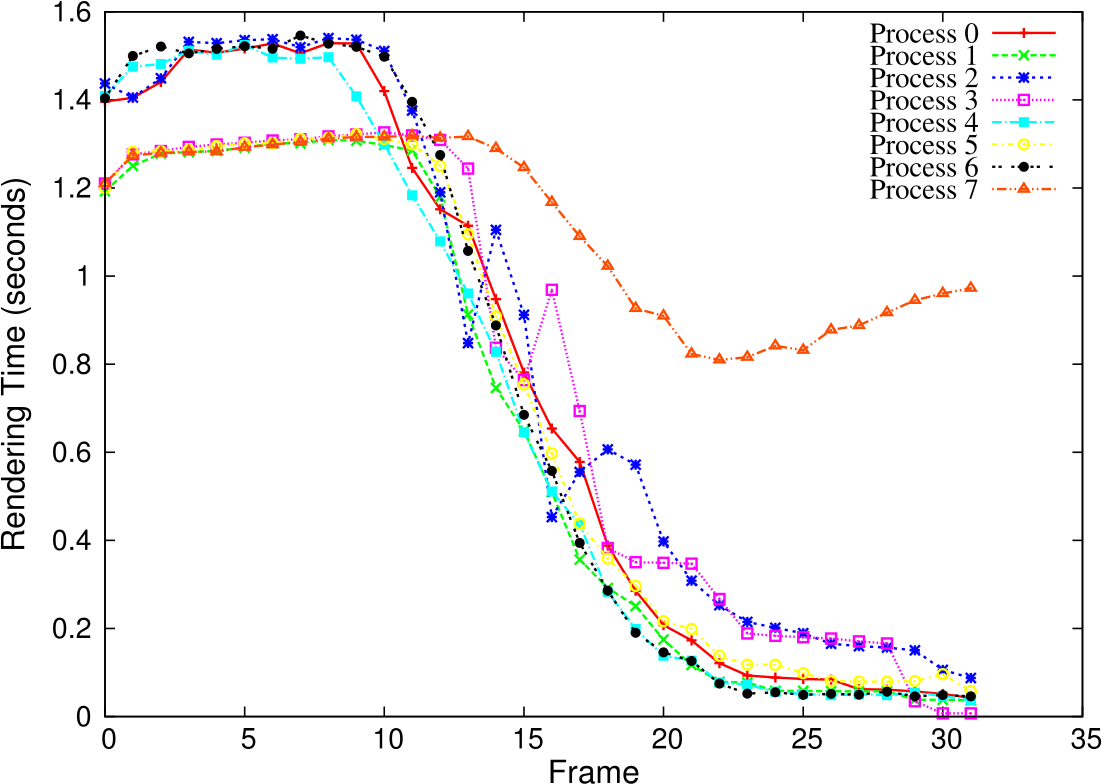
\includegraphics[width=\linewidth]{images/multiscale/mueller}

  \caption{Per-process rendering times for the `M\"uller' line given in
  Figure~\ref{fig:balance}}
  \label{fig:mueller}
\end{figure}

This was apparent in the tests described in Figure~\ref{fig:balance}:
the algorithm balanced between some of the nodes, but the slowest node
was never balanced, and therefore the user-visible performance fror
this run was
equivalenty to the static case.  Figure~\ref{fig:mueller} shows a more
detailed analysis of the execution of the M\"uller algorithm that
generated the data in
Figure~\ref{fig:balance}.  The per-node rendering times in
Figure~\ref{fig:mueller} show that process 7 is usually the last
process to
finish and is often \emph{considerably} slower than the next-to-last.
As evident from the lack of sudden discontinuities in process 7's
rendering times, however, no bricks from process 7 move to other nodes.
Rendering times decrease across other nodes, but the maximum rendering
time does not change.

We theorize that additions to the algorithm to learn weights for each
individual brick would yield friutful results.  Furthermore, the algorithm
explicitly attempts to avoid visiting the entire tree, as an attempt to bound
the maximum time needed to determine a new balancing.  In our work, we did not
observe cases where iterating through nodes in the tree had a measurable
impact on performance, and feel that  by doing so the algorithm could obtain
the global knowledge it needs to balance data effectively.  Both of these
extensions are left for future work.

In Section~\ref{sec:introduction} we noted a variety of quesitons that the
design of our system allows us to answer.

\begin{itemize}

  \item \textit{Rendering vs. compositing}.  As shown in
  Table~\ref{tbl:breakdown}, subsecond rendering times are achieved
  using a very small number of nodes, relative to previous work.  This
  relieves a significant source of work for compositing algorithms.

  \item \textit{Overhead of GPU transfer}.  Table~\ref{tbl:breakdown}
  shows readback time to be on the order of thousandths of a second for
  common image sizes.  Measuring texture upload rates is difficult due
  to the asynchronous nature of OpenGL and current drivers, but we did
  not find evidence to suggest this was a bottleneck.

  \item \textit{Importance of load balancing}.  A dynamic load balancer
  can have a worthwhile impact on perfprmance.  However, it can also
  lower the performance of the system.  Load balancers generally come
  with some number of tunable parameters, and useful settings for
  these parametrs are difficult to determine \textit{a priori}, and
  likely impossible for an end-user to effectively set.  We observed
  that dynamic load balancing for volume rendering struggled in cases
  often encountered in real-world environments and, for this reason,
  believe there is still a gap before deploying these techniques in
  \emph{production} systems.  There is a great opportunity for future
  work in this area.

  \item \textit{Viability}.  As displayed in Figure~\ref{fig:rtime} and
  Table~\ref{tbl:breakdown}, rendering extremely large data sets---up
  to $8192^3$ voxels---is possible on relatively few nodes.  Further,
  data sets up to $2048^3$ can be rendered at an interactive two frames
  per second.

\end{itemize}

\section{Conclusions}
\label{sec:conclusions}

With this study, we demonstrated that GPU accelerated rendering
provides compelling performance for large scale data sets.
Figure~\ref{fig:rtime} demonstrates our system rendering data sets
that are among some of the largest reported thus far, using far fewer
nodes than previous work.  This work shows that a multi-GPU node is a
great fojundational `building block' to compose larger systems cpaable
of rendering very large data.  As the price-performance ratio of a
GPU is better (provided it can effectively parallelize the workload)
than CPU-based solutions, this work makes the case for spending more
visualization supercomputing capital on hardware accleration, and
acquiring smaller yet more performant clusters.

Reports on the time taken for various pipeline stages demonstrate that
PCI-E bus speeds are fast enough that readback performance is not as
great of a concern as it was a few years ago.  Howeever�, it remains to
be seen if contention will become an issue if individual nodes are made
`fatter', utilizing additional GPUs.  The 1 GPU per node given in
Figure~\ref{fig:rtime} suggest that multiple GPUs do contend for
resources, but at this scale the differences are not yet significant
enough for warrant moving away form the more cost-effective `fat'
node architecture.  Given the relatively few nodes needed for good
performance on large data, and external work scaling compositing
worklaod out to tens of thousands of cores, it seems likely that the
relatively `thin' 2-GPU-per-system archietcture can be made to scale
to even larger systems.

We would like to study our system with higher image resolutions, such
as those available on a display wall, and larger numbers of GPUs. At
some point, we expect compositing to become a significant factor in
the amount of time needed to volume render large data, but we have
not approached the cross-over point in this work, due to the use of
`desktop' image resolutions and low numbers of cores.

Our system allows substituting a Mesa-based software renderer when
a GPU is not available. This provided a convenient means of
implementation for an existing large software system, in particular
because it allows pipeline execution to proceed unmodified through
the rendering and compositing stages. However, tests very quickly
showed that using software renderers when a GPU was available was
not worthwhile, and usually ended up hurting performance more than
helping. Therefore, we traded access to more cores for the guarantee
that we will obtain GPUs for each core we do get.

An alternate system architecture would be to decouple the rendering
process from the other work involved in visualization and analysis,
such as data I/O, processing, and other pipeline execution steps. In
this architecture, all nodes would read and process data, but
processed, visualizable data would be forwarded to a subset of nodes
for rendering and compositing. The advantage gained is the ability to
tailor the available parallelism to the visualization tasks of data
processing and rendering, which, as we have found, can benefit from
vastly different parallel decompositions. The disadvantages are the
overhead of data redistribution, and the wasted resources that arise
from allowing non-GPU processes to sit idle while rendering.

Our compositing algorithm assumes that the images from individual
processors can be ordered in a back-to-front fashion to generate the
correct image. For this paper, we met this requirement by using regular
grids, which are easy to load balance in this manner. It should be
possible to also handle certain types of curvilinear grids and perhaps
AMR grids.  Extensions to handle unstructured grids would be difficult,
but represent an interesting future direction.

Load balancing is an extremely difficult problem, and we have just
scratched the surface here. The principal difficulty in load balancing
is identifying good parameters to control how often and to what extent
the balancing occurs. We would like to see ideas and algorithms
which move in the direction of user-friendliness: determining the
most relevant parameters and deriving appropriate values for them
automatically.


\chapter{Large-scale data access}
\label{chp:io}
While additional cores and newer architectures, such as those provided
by GPU clusters, steadily increase available compute power, memory
and disk access has not kept pace, and most believe this trend will
continue.  It is therefore of critical importance that we design
systems and algorithms that make effective use of off-processor
storage.  This work details our experiences using parallel file
systems, details performance using current systems and software,
and suggests a new API that has greater potential for increased
scalability.

\section{Introduction}

Large scale parallelism is widely used not only to simulate complex
phenomenon, but also to process the resultant data for understanding
and insight.  Parallel visualization and analysis applications exist
to aid in this process, but I/O performance analysis generally takes
a back seat to other metrics, such as renderer performance, with the
justification that one only reads the data once and then spends much
more time interacting with it.  However, as we scale visualization
tools up, we find that the time taken for the initial reading of
the data is prohibitive, and becomes a significant barrier to the
scientist's task: to understand their data and gain new insight in
their science.

In developing any application, there are a number of practical
concerns that must be considered to obtain acceptable performance.
In the space of I/O, and especially distributed filesystems, many
visualization and analysis developers pay little heed to these
concerns.  In this work we hope to elucidate some `best practices' for
writing applications that will utilize parallel filesystems, as well
as steer a convergence between application and filesystem developers.

\subsection{Previous Work}

Since the performance of most large scale visualization systems is
clearly bound by I/O performance a significant body of literature
exists to analyze and improve this component of parallel software.  We
provide a brief overview of a subset of that literature here.

The predominant file systems in use in modern supercomputers are the
Network File System (NFS) filesystem and Lustre.  NFS was originally
developed by Sun and is now in its fourth revision.  However, despite
the third revision's release almost twenty years
ago\cite{Callaghan:1995:NFSv3,Hildebrand:2004:NAHP}, it is still in
wide deployment.  The ``Linux Cluster'' filesystem,
Lustre\cite{Sun:2008:PSIW}, is a newer filesystem that distributes
the I/O workload across multiple nodes, and thus has been demonstrated
to scale considerably better.  Both systems have characteristics that
should inform how we develop software to run on such systems.  We focus
this work on these two filesystems due to their prevalence in high
performance computing environments.

Collective I/O (CIO)~\cite{Nitzberg:1995:PIO, Seamons:1995:SDCI,
Kotz:1997:DIMF} was introduced as a very versatile concept where the
I/O bandwidth is increased by coalescing a number of I/O requests to be
sent to the storage system as a single large request.
Memik et al.~\cite{Memik:2002:EIA} extended CIO as Multi-Collective
I/O (MCIO) by optimizing I/O accesses to multiple arrays
simultaneously. They show that optimal MCIO patterns require the
solution to an NP-complete problem but are able to demonstrate up to
85\% speedups over CIO using a heuristic approach.

A similar concept was recently presented by Kendall et
al.~\cite{Kendall:2009:TDO}. They showed that, with a carefully chosen
greedy algorithm, end-to-end access times of under a minute are
possible in the visualization of terascale data.  Their system accessed
multi-file netCDF~\cite{Rew:1990:NAIF} data using the Parallel netCDF
library~\cite{Li:2003:PNAH} that is in turn built on top of MPI-2
\cite{Gropp:1998:MTCR}.

Lofstead et
al.~\cite{Lofstead:2008:FIAI,Lofstead:2009:AMRI,ADIOS:Manual} report
that on current supercomputers, independent I/O tends to outperform
collective I/O. They present the ADaptable IO System (ADIOS) and ---
in combination with MPI-IO and collective MPI-IO --- report speedups
of about an order of magnitude compared to a serial HDF5 access. To
improve access to data stored in HDF5
Howison et al.~\cite{Howison:2010:THFL} present optimizations for the
Lustre File System.

Specifically targeting scientific visualization of large-scale
earthquake simulations on parallel systems, Ma et
al.~\cite{Ma:2003:VVLS} demonstrated that overlapping I/O with
rendering can significantly reduce inter frame delay. This concept was
extended into a general parallel visualization pipeline for large
earthquake simulations by Yu et al.~\cite{Yu:2004:PVPF}.

Yu et al.~\cite{Yu:2008:PADP} conducted an extensive characterization,
tuning, and optimization of parallel I/O on Jaguar, a Cray XT based
supercomputer at Oak Ridge National Laboratory that uses Lustre
\cite{Sun:2008:PSIW} for its IO subsystem.

Yu et al.~\cite{Yu:2004:ISFP} demonstrated general I/O solutions
for the visualization of time-varying volume data in a parallel and
distributed computing environment.

Peterka et al.~\cite{Peterka:2009:ETES} also present optimization
strategies for the problem of volume rendering large time dependent
datasets, focused specifically on the IBM Blue Gene/P system
system. Their summary result is that even with optimized storage and
access systems I/O still severely limits the overall performance and
more research is required in this area.

Recently, Lang et al.~\cite{Lang:2009:IPCA} performed a comprehensive
study of I/O on Intrepid, the IBM Blue Gene/P system at the Argonne
Leadership Computing Facility. In their work they also give a broad
overview of existing parallel file system evaluations and HPC system
scaling studies.

Ching et al. contribute a a more modern take on file and range locking
in distributed filesystems~\cite{Ching:2007:Locking}.  Using their
distributed lock manager, they demonstrate scalability up to 32
servers, something the POSIX locking model cannot provide.

\subsection{Contribution}\label{sec:contribution}

Our primary goal with this work is to inform developers writing
visualization and analysis applications on the characteristics of
I/O systems at a multitude of scales.  We desire to show methods by
which parallel applications can be written to maximize performance for
developers' constituency, without working directly with their user base
or clusters that the application will run on.  As a community, we will
never have the resources required to address the specific machines that
every supercomputing-based science group needs to utilize.  Therefore
we must design applications that perform well on such machines without
investing weeks (or months) of a visualization or I/O expert's time to
achieve that performance.

Most I/O studies focus on a particular machine and even a specific
application on that machine.  This approach would not, however,
serve our purpose of identifying I/O best practices that are widely
applicable.  We contribute end-to-end scalability results of a typical
analysis problem on volume data, for numerous clusters and a variety of
I/O backends.

Finally, based on our work developing parallel visualization and
analysis applications like the one in this work, we propose an
extension to the ubiquitous POSIX API that has the potential to
greatly improve the performance of parallel I/O systems.

The remainder of this paper is organized as follows.  First, we review
some disk and I/O characteristics that are common to both serial and
parallel environments.  In Section \ref{sec:parallel_fs} we describe
filesystems in common use in modern cluster computing environments.
Then we expound the design of a program that has I/O as a major
component, and describe implementations using numerous backend APIs, in
Section \ref{sec:access}.  In Section \ref{sec:design} we use the
knowledge gained in Sections
\ref{sec:parallel_fs} and \ref{sec:access} to enumerate an API that
would allow improved scalability on current and future parallel
filesystems.  Finally, we conclude by highlighting the limitations,
drawbacks, and opportunities for mistaken conclusions that arise due
to our methods.

\section{Data Access Time}\label{sec:basics}

The overall time to perform any I/O operation is well studied.
Generally we consider this to follow the simple equation:
\begin{align*}
  T_{total} = T_{access} + T_{trans}
\end{align*}
that is, the total time to perform an I/O operation is equal to the
time to seek to the desired track along with the time for the start of
the needed sector to spin under the disk head, plus the time for the
platter to spin until all the required sectors have passed under the
head.

We will utilize a hypothetical modern disk with an average access
time of 8 msec, and a sustained transfer rate of 100 MB/s. The access
time time is a conservative median for current consumer level disk
drives. The 100 MB/s sustained transfer rates are not yet possible with
current consumer level disks, but the number is close enough and serves
our purpose well.

\begin{figure}
  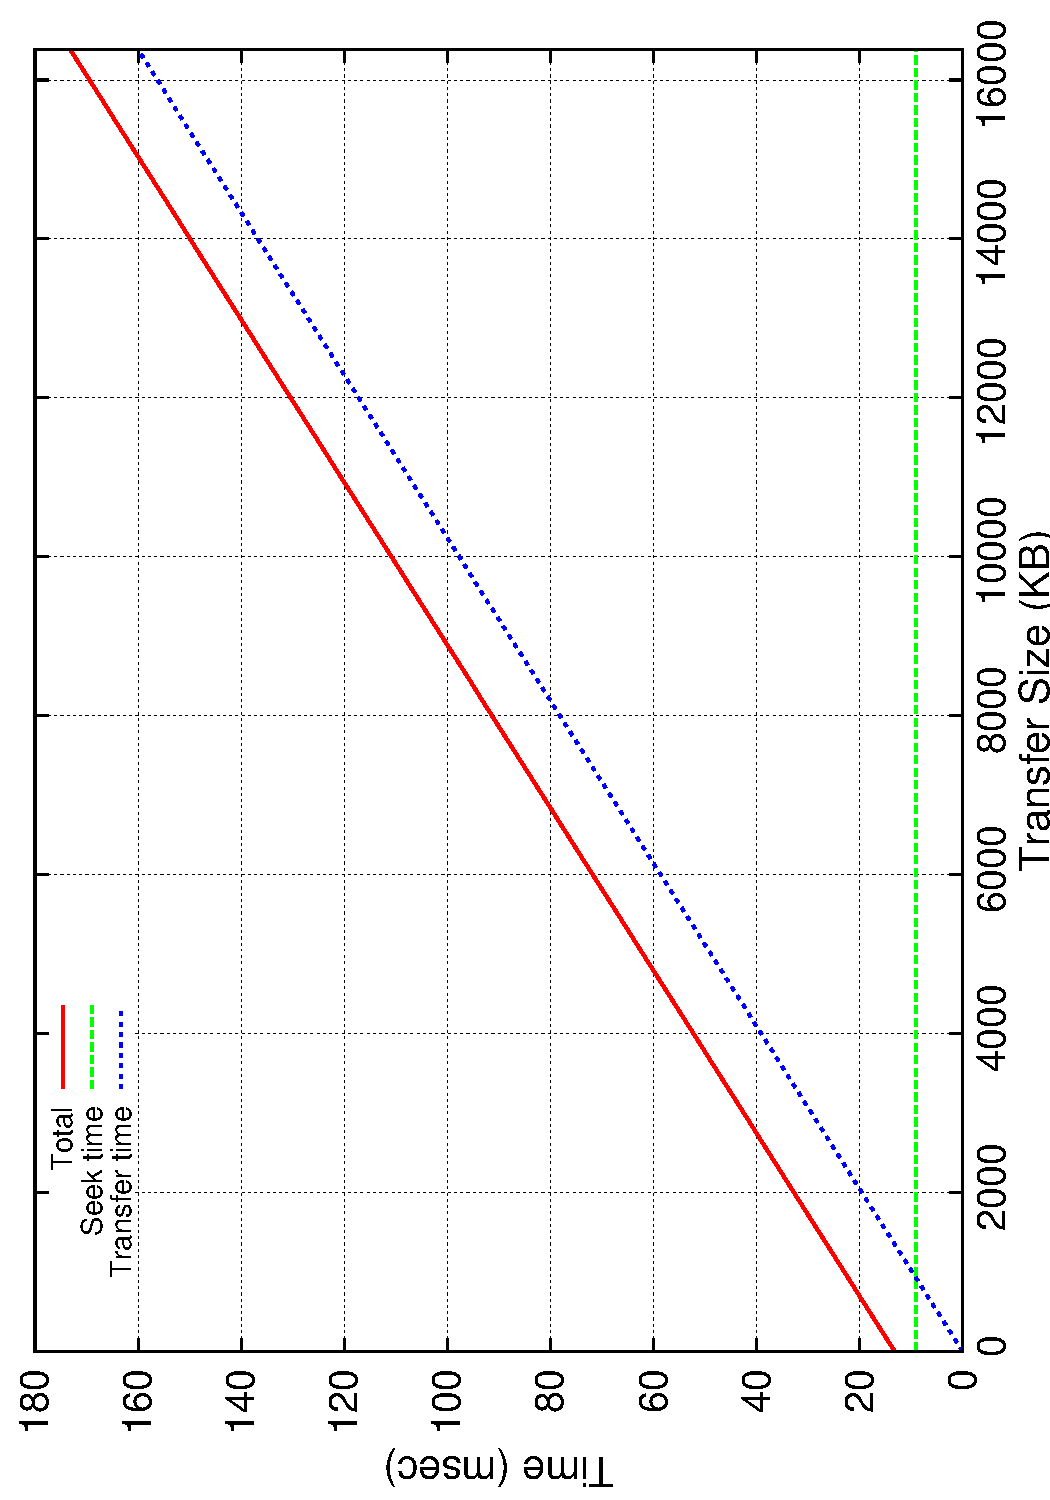
\includegraphics[angle=270,width=\linewidth]{images/io/io-overall}
  \caption{Total I/O time as a function of transfer size.  Transfer rate
  quickly overtakes access time.}
  \label{fig:io-total}
\end{figure}

%%%% It the transfer rate section goes this one should follow
%Since it is very hard to optimize for $T_{rotational}$ we will
%focus on seek time and transfer time optimizations in the following
%sections.

\subsection{Considerations for access time optimizations}

The total time to transfer data of $M$ MB can
be described by the equation:
\begin{align*}
  T_{total} =  \frac{T_{\text{access}}}{1000} +  \frac{M}{R_{\text{trans}}}
\end{align*}
where $R_{trans}$ denotes the transfer rate in MB per second. 
We divide $T_{access}$  by 1000 to express it in seconds as it is
normally given as milliseconds.
Consequently, the access time represents a percentage $P$ of the overall time
that can be expressed as:
\begin{align*}
P &= 100 \cdot \frac{T_{\text{access}}}{T_{\text{total}} \cdot 1000}
\\&=  \frac{T_{\text{access}}} {\frac{T_{\text{access}}}{100} +  10 \cdot \frac{M}{R_{\text{trans}}}}
\end{align*}
If we now insert the parameters of the above described hypothetical
disk and assume that we are partitioning our data in 10 MB blocks we
arrive at the consclusion that---when we need to do a random seek
operation for every single block of data---the seek time accounts for
only 7\% of the overall time to access the data.

Now, to assess the gain of a specific layout scheme we consider the following 
equation. It measures the performance gain $G$ in percent for a given scheme if that scheme reduces 
random access by a factor of $F$.

\begin{align*}
G  &= 100 \cdot F \cdot \left( \frac{ \frac{T_{\text{access}}}{1000} + \frac{M}{R_{\text{trans}}} }{\frac{M}{R_{\text{trans}}}}- 1\right)
\\ &= 100 \cdot F \cdot \frac{ \left(\frac{ T_{\text{access}} } {1000}\right)}   { \left(\frac{M}{R_{\text{trans}}}\right)}
\\ &=  \frac{F}{M} \cdot \frac{T_{\text{access}} \cdot {R_{\text{trans}}}  }   { 10 }
\end{align*}

Again, assuming the hypothetical drive parameters from above and we get

\begin{align*}
G  &=   \frac{F}{M} \cdot 80
\end{align*}

For a scheme that reduces random access by a factor of 3, only a 2.6\%
improvement in runtime would be achieved for 10 MB blocks, while with the same scheme
the performance would be almost tripled with 900 byte blocks.

From these numbers we conclude that in most environments, in particular
those with structured data---where larger data blocks can be
utilized more easily---a data layout optimization would only improve
a very small fraction of the overall time and is most likely not worth
the implementation and
maintenance effort. For environments that \emph{must} break the data into
tiny chunks a clever layout strategy to improve data access times can in the
best case (in which the majority of disk operations involve seeks) double the
data access performance.

%%%% moved to ``The takeway:'' to make it more consistent with the 
%%%% rest of the paper
%Looking at the above results from a different perspective, we can derive the
%rule of thumb that as long as data is broken into pieces larger than 10 MB
%no special care needs to be taken on a consumer HDDs about the data layout.  

It is worth noting that with the advent of solid state drives, in
particular for consumer workstations, this minimal block size required
to utilize unwrought data layout strategies while still obtaining
good performance is bound to shrink even more, as those drives have a
significantly smaller `seek' time with only moderately higher transfer
rates.

Finally, it should once again be stressed that the percentages
given above account for maximum theoretically possible optimization
potentials if all seek operations could be completely avoided and no
other additional overhead would come from the layout.  In reality the
speedup that can be gained from access time optimization will stay
below that value. In particular it is worth noting that accessing data
via optimized layout schemes does not come
for free. Kendall et al.~\cite{Kendall:2009:TDO} demonstrated for
distributed memory systems that a random ordering scheme outperforms
most space filling curve approaches.

The takeway:

\begin{itemize}
  \item If the data is broken into pieces larger than 10 MB, then it
  is not worth worrying about the data layout for even consumer level
  disks.
  \item For kilobyte sized chunks a clever layout strategy can
           significantly cut the data access time on a standard HDD.
\end{itemize}

\section{Parallel Filesystems}\label{sec:parallel_fs}

All distributed filesystems have unique characteristics that should
inform the way we access and process data.  In this section we
will highlight some of the common pitfalls that may be found with
applications designed to run in an NFS or Lustre environment.

\subsection{Opening Files}

Opening a file is one example of an operation that performs uniquely
in a distributed environment.  In NFS systems, this is implemented
via the client sending an \verb!ACCESS! or \verb!GETATTR! remote
procedure call.  The operation asks the server if the client is allowed
to access the file, or requests metadata for the file.  The server
responds with a small message containing the resulting permissions.
The situation in Lustre is similar: queries go to a global `metadata
server' (MDS) that grants or denies access.  In both systems,
\emph{the file is not opened}.  Doing so would consume resources on
the server, particularly due to read-ahead caching, and the request
to actually read or write the file may be significantly delayed in
time---or might never come at all!

%\begin{figure}[Htb]
%  \centering
%  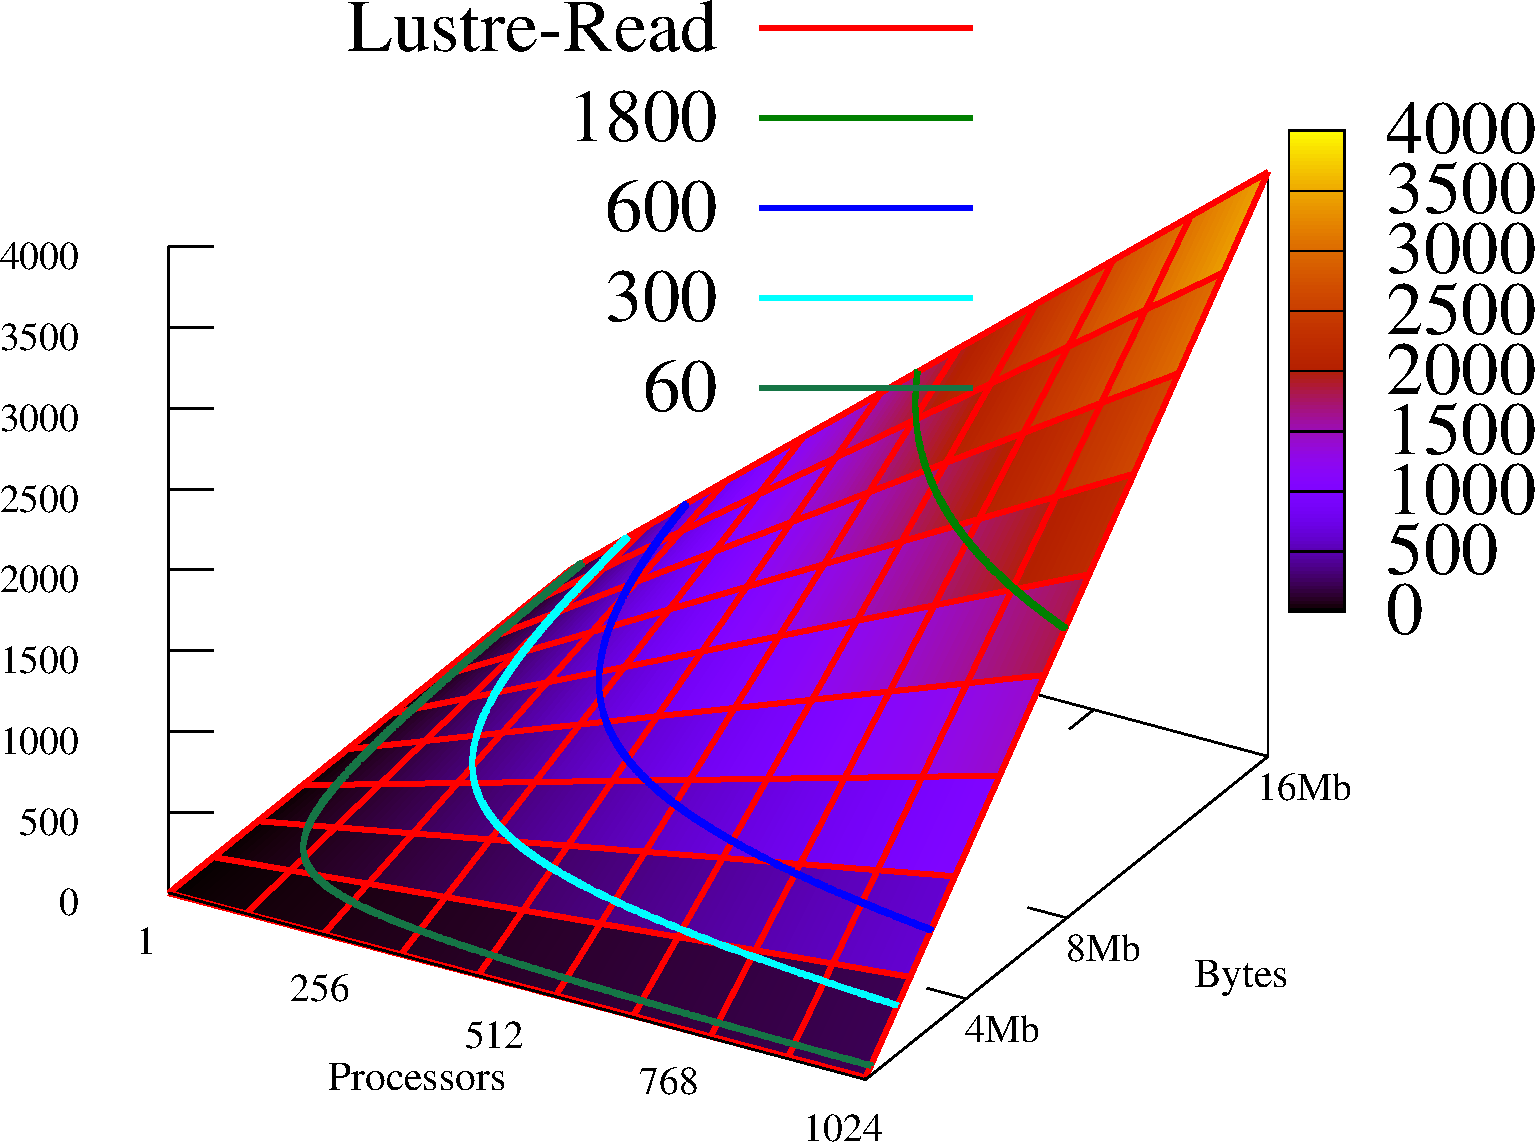
\includegraphics[width=\linewidth]{images/io/lustre-read}
%  \caption{Best case read performance with Lustre.}
%  \label{fig:lustre-read}
%\end{figure}
%
%\todo{Can we fit/justify Figure \ref{fig:lustre-read} in here somehow?  It's
%such a pretty graph ;)}

This has important implications for programs running on such
filesystems.  Any distributed filesystem is going to scale extremely
poorly with a program that opens many files at one time.  Since the
\verb!open! call must correctly report errors, the request and response
must be entirely synchronous.  There is no \verb!openv! system call in
POSIX, analogous to \verb!readv!.  Therefore every open file request
must send a (very small) message to a server, and wait for a (very
small) message to return.  The network capacity for messages at these
sizes is extremely poor.  It is important to note that \emph{Lustre
does not scale any better than NFS} in this use case, as it has the
singular bottleneck of one MDS per filesystem.  Many sites split up
their Lustre offerings into multiple filesystems as a way to mitigate
this problem, but these must then be mounted under different
locations in the filesystem hierarchy.

To prevent inducing poor performance in this manner, avoid opening
more than one or two files per process; at large scale,
even that will be a bottleneck.  Furthermore, if at all possible,
avoid synchronization points immediately before opening files: if one
absolutely needs an \verb!MPI_Reduce!, for example, try opening the
file immediately before the reduce instead of immediately after.  This
should prevent a `thundering herd' (to steal a term from the threading
world) of processes that pound on the metadata server at the same
time.  It is interesting to note that the ADIOS middleware library
already attempts to mitigate this effect~\cite{ADIOS:Manual}.

The takeway:

\begin{itemize}
  \item At large scale, eschew large numbers of files.
  \item Stagger synchronization points with \verb!open! calls.
\end{itemize}

\subsection{Closing Files}

Distributed filesystems almost unilaterally implement what is referred
to as `close-to-open cache consistency'.  To increase performance,
writes are cached locally on the client filesystems.  During regular
intervals or in response to certain events, the client cache is flushed
to the server.

This presents difficulties in implementing \verb!write!s.  The problem
is in reporting errors when a write should fail; since the system only
writes to a local cache, the write never reaches its final destination
and thus additional errors could still occur after the user process has
proceeded beyond the write.  It is possible for the write to be sent to
the server machine, enter into the server's cache, and eventually be
denied due to a transient error (e.g. exceeding quota).  Yet the client
system cannot report this error to the running process, because the
process has long since moved on from the failing write call.

Distributed filesystems thus require a client cache to write-through
all changes when the client application \emph{closes} the file.  Client
operating systems must get a confirmation from the server that all data
has been flushed
\emph{before} it returns from the client processes' \verb!close!
call; this is the last possible operation for the file, and thus the
distributed systems' final opportunity to report errors that may
indicate data loss.

It is therefore highly desirable to delay close operations that occur
after writes.  If a process is writing multiple output files, try to
make it maintain two open files instead of one, and close the file from
the previous iteration while writing in the current iteration.

Sadly many applications, even those designed to run on supercomputers,
do not check the return value of the \verb!close! system call.  There
is no reason to believe that what was written is consistent, given
such applications.

The takeaway:

\begin{itemize}
  \item \emph{Always} check \verb!close! for errors!
  \item Try to delay \verb!close!s that appear after \verb!write!s.
\end{itemize}

\subsection{Locking}

By `locking' here we are referring to advisory file locking, a la
the \verb!flock! system call; mandatory file locking has its own
set of issues in even a serial environment, and the utility of such
locking in an HPC environment is nebulous.  In our experience, few
if any large scale visualization and analysis applications utilize
file locking.  However, it is worth noting that locking typically
adds an I/O synchronization point, much like \verb!close! would.  For
this reason it is not recommended that an application lock and unlock
files unless there is an interaction with known external software
that dictates it.  If at all possible, a better solution would be to
\verb!close! the files on the writing process, and send a message to
reading processes notifying them that the writer has completed---before
they attempt \verb!open!ing the files at all.

Locking can in theory provide the best mechanism for inter-process
communication in a distributed environment (i.e. to coordinate with in
situ visualization and analysis processes), however it is not in wide
use, perhaps due to the issues mentioned here.  As noted
earlier~\cite{Ching:2007:Locking}, this is still an area of research
in HPC systems and so we recommend the aforementioned explicit
synchronization methods for now.

\section{Parallel Data Access}\label{sec:access}

To identify the ideal method for accessing data in numerous
environments, we wrote test programs using a variety of APIs and
API options, then evaluated their performance.  Yet many scientific
visualization and analysis packages, in addition to large scale
simulation software, utilizes some I/O middleware for data access.
These middleware packages offer complexity reduction, and typically
provide a method for ascribing higher level metadata with data, such as
the dimensionality and mesh information.  After identifying the ideal
low-level methodologies, we sought to quantify the differences between
middleware libraries, and in particular their scalability on distinct
clusters.

To quantify this, we developed the same analysis program using
a variety of backend APIs.  The program is simple: it is a
threshold-based volume segmentation tool.  The software reads in a
large volume and outputs a binary mask volume that indicates the
voxels that fall between the threshold values.  The program is
parallel, and out-of-core: the input volume is intelligently bricked,
and each process is responsible for a set of bricks.  Processes load up
a brick and generate the output volume brick one at a time.  We chose
out-of-core as opposed to in-core because it models how future (even
current) visualization and analysis software must be written, given the
current trend of increasing processing-power-to-memory ratios.

\subsection{Results}

We ran our application on multiple distinct supercomputers.  One
cluster is specifically designed for visualization; another excelled at
analysis; the third is a very large scale general purpose supercomputer
designed for `leadership computing'.  Installation dates were diverse:
one cluster was commissioned in 2008, another went into production
early in 2010, and a third was originally installed in 2005, receiving
its most recent upgrade in 2009.  All of these clusters are using
Lustre for their backend filesystem.  On all systems, we used the
`native' compilers and, where available, system-installed modules for
the libraries we required.

% lens: installed may 2008 (analysis)
% longhorn: production on jan 4th 2010 (visualization)
% jaguar: installed 2005, upgraded late 2009 (general purpose)

For backend I/O we tested multiple configurations: NetCDF, HDF5/NetCDF,
and a custom solution.

The hierarchical data format (HDF) is a data model that has seen
significant uptake in the parallel computing world.  It provides
mechanisms for organizing complex data in an extensible manner.  We did
not look directly at HDF5, but instead considered it in concert with
NetCDF.

\begin{figure}
  \centering
  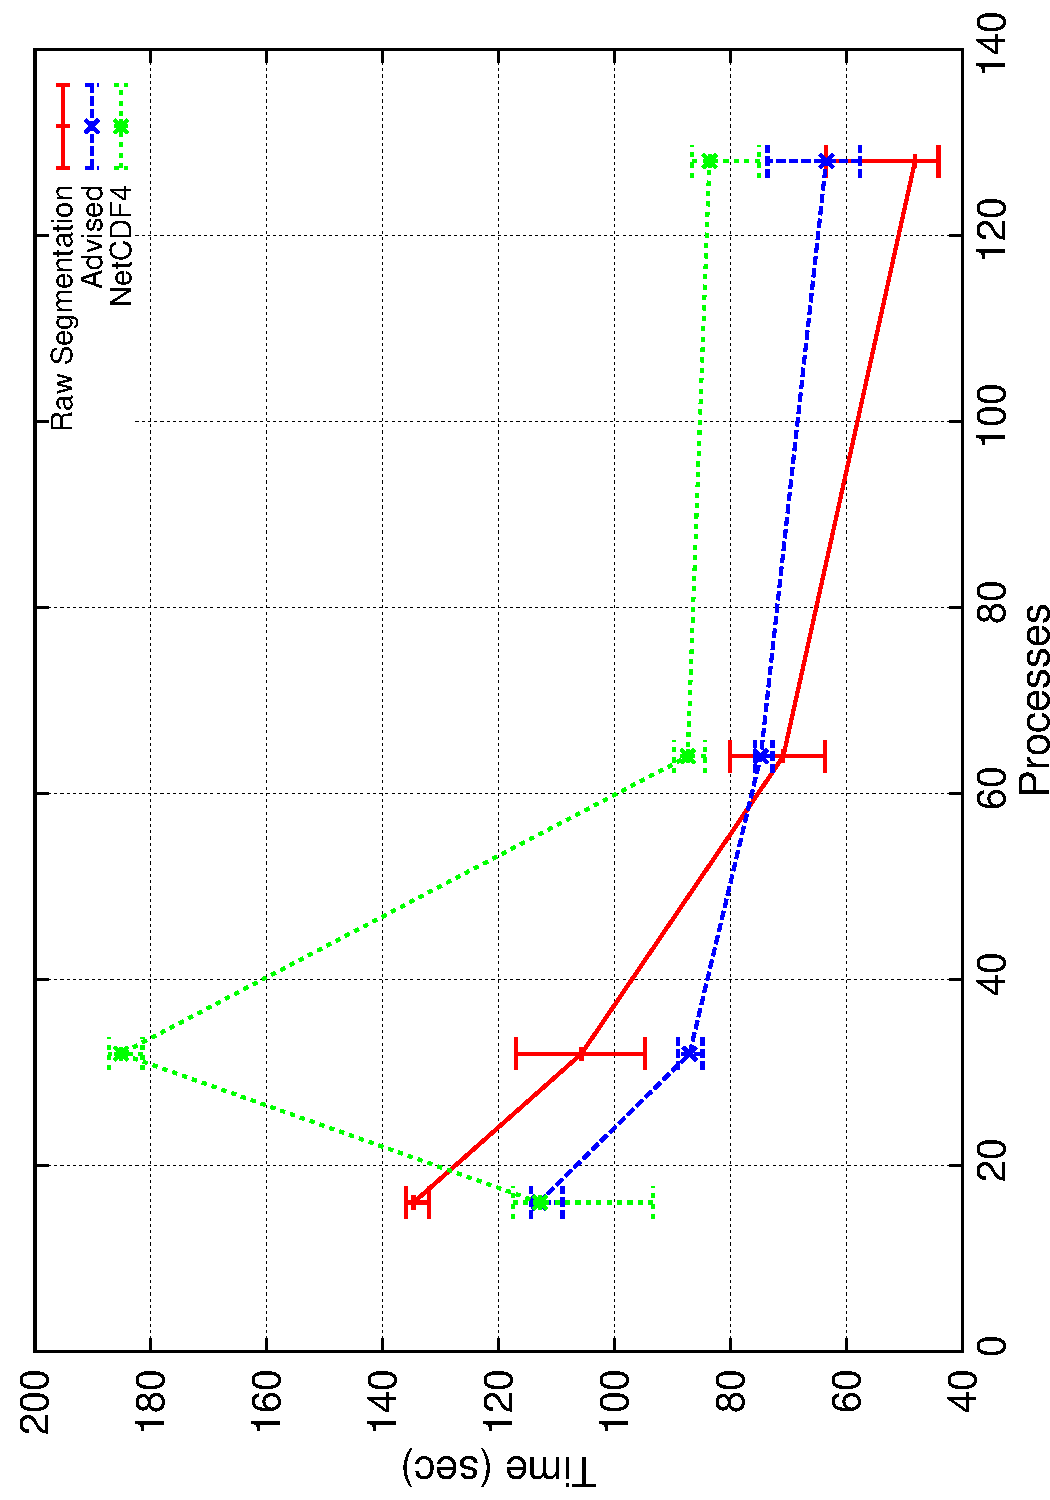
\includegraphics[angle=270,width=\linewidth]{images/io/lens-most}
  \caption{Strong scaling of our example segmentation program running
  on cluster \#1, with a variety of I/O backends.  `NetCDF4' is NetCDF
  with an HDF5 backend.  `Raw' is our hand-generated simple I/O layer,
  and `Advised' a minor modification on it.  Error bars indicate
  maximum and minimum running times per process in the job.}
  \label{fig:lens-most}
\end{figure}

The Network Common Data Form is a library that provides array-oriented
data access.  Like HDF5, NetCDF files endeavor to be partly
self-describing.  With recent releases of the NetCDF library, there
are a multitude of options for backend I/O.  The first is so-called
`classic' NetCDF files.  These files have a limit of 2Gb per variable,
and thus were not considered for this study.  The `64bit offset' format
is an extension of the `classic' format to allow use of 64bit indices,
and thereby to address files of, for all practical purposes, unlimited
size.  The final format is the so-called `NetCDF4' format -- somewhat
confusing because the `64bit offset' format debuted in 3.6.0, right
before the 4.0 release, yet is a distinct backend that uses HDF5 as
its backend.  To disambiguate, we refer to the `64bit offset' format as
``NetCDF-64'' and the HDF5-backed format as ```NetCDF4'' in this work.

We also developed a custom I/O layer based on our experiences on a
variety of machines, including workstations.  The approach is very
simple: each process memory-maps a chunk of the large input data file,
as well as the relevant portion of the output mask file.  Data are
processed out of the memory-map as is, without intermediate buffers.
The source for this version is thus simpler than any other version of
the program, containing no memory management code for data buffers.  As
such, this version required the least memory by a wide margin: the API
dictated an approach that was naturally out-of-core.

The results on the first cluster can be seen in Figure
\ref{fig:lens-most}.  `NetCDF4' is NetCDF backed with an HDF5 file.
`Raw segmentation' uses our custom I/O layer based on \texttt{mmap}.
`Advised' is the `Raw' line, with the addition of just a single line of
code, placed before we process a block of data:
\begin{verbatim}
  posix_fadvise(fd,
    index * sizeof(float),
    buffer_size,
    POSIX_FADV_WILLNEED
  );
\end{verbatim} That is, we are informing the operating system that
we will need block $X+1$ in the near future, just before we begin
processing block $X$.  We had found that including this optimization
increases our performance 3 to 4x on desktop systems.  Results on the
supercomputer do show an initial increase in performance, but the
effect was unfortunately subdued at higher concurrency.  We do not
include results for the NetCDF-64 run in this figure, as it did not fit
in the same scale as the pictured backends.

Results for this machine were somewhat difficult to report, because
they varied so widely.  We ran the scaling study for one particular
format straight through, with no delays between runs, multiple
times.  In each instance the NetCDF4 result included a spike in the
running time.  For our raw segmentation, we would see results offset
by 20 seconds or so, and the width of the error bars would change
arbitrarily.  The readahead version of the program experienced less
variability, but we were unable to conclude whether this was a property
of the program or simply luck.  The data presented in figures
represents the \emph{set} of runs that performed best overall, for
that I/O backend.

\begin{figure}
  \centering
  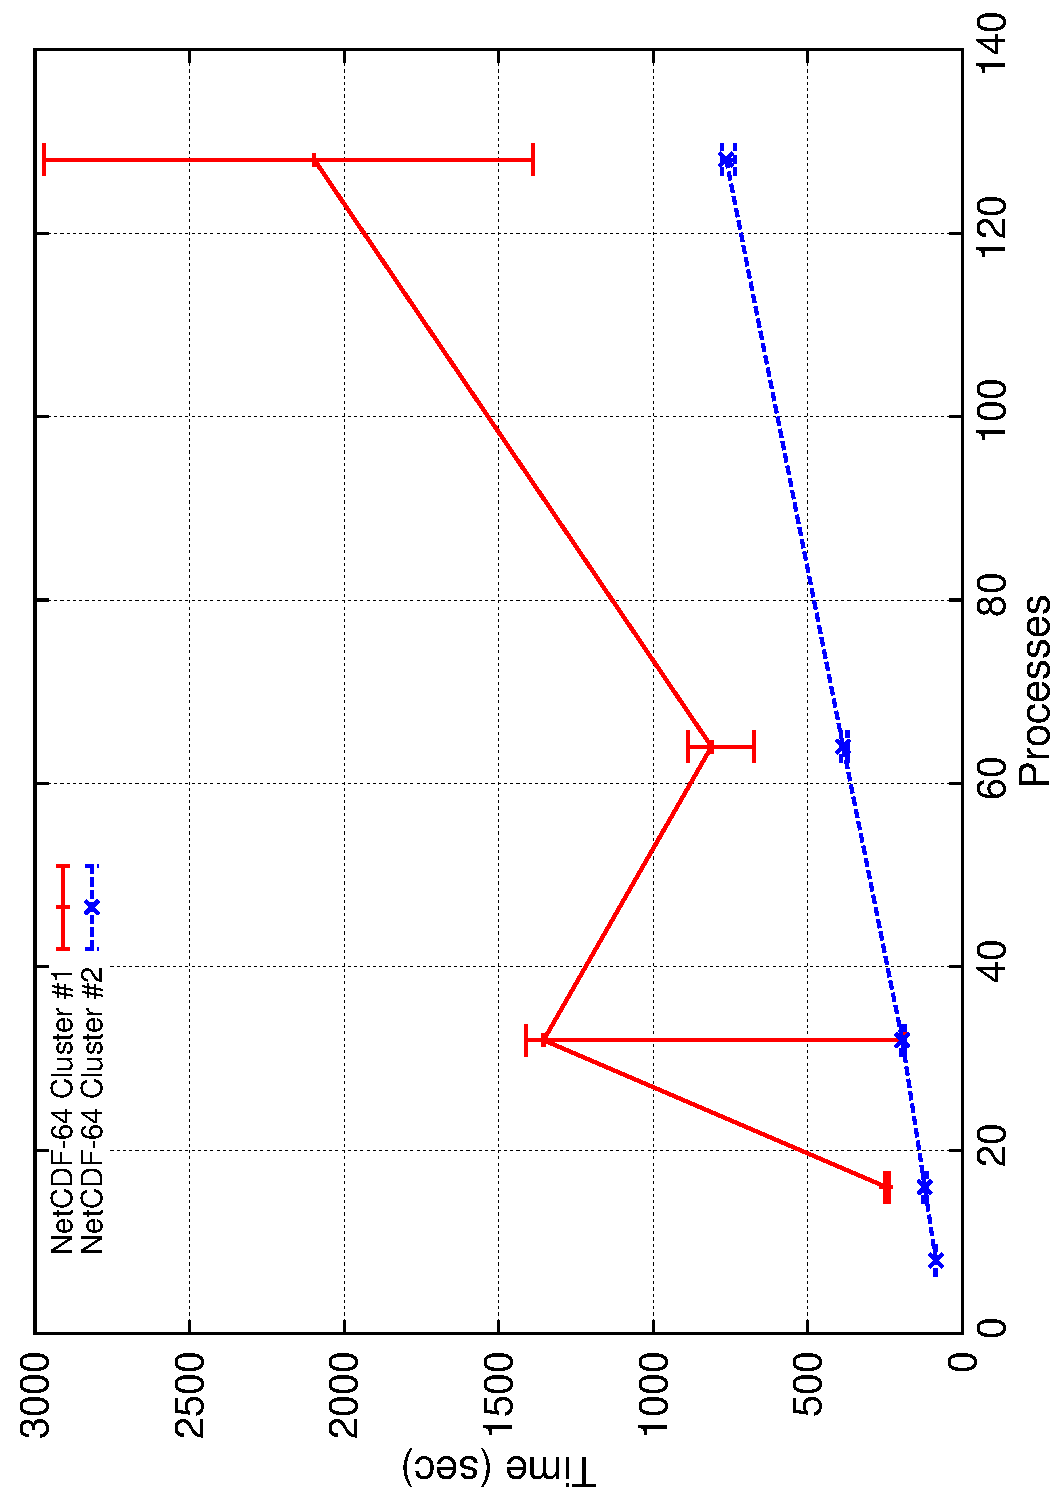
\includegraphics[angle=270,width=\linewidth]{images/io/n64}
  \caption{Strong scaling using the NetCDF `64bit offset' file format
  on multiple clusters.  Higher levels of concurrency led to decreased
  overall performance when using this format.  Of note is the high
  variability from cluster \#1, characteristic of that machine's I/O
  subsystem.}
  \label{fig:n64}
\end{figure}

The NetCDF-64 results could not be plotted with the other results, due
to the large difference in scale.  Results using this format on
multiple clusters is provided in Figure \ref{fig:n64}.  Performance
actually decreased with this backend.  For this reason, we highly
recommend forcing the HDF backend (using the \texttt{NC\_NETCDF4} flag)
when writing applications that make use of the NetCDF API.

\begin{figure}
  \centering
  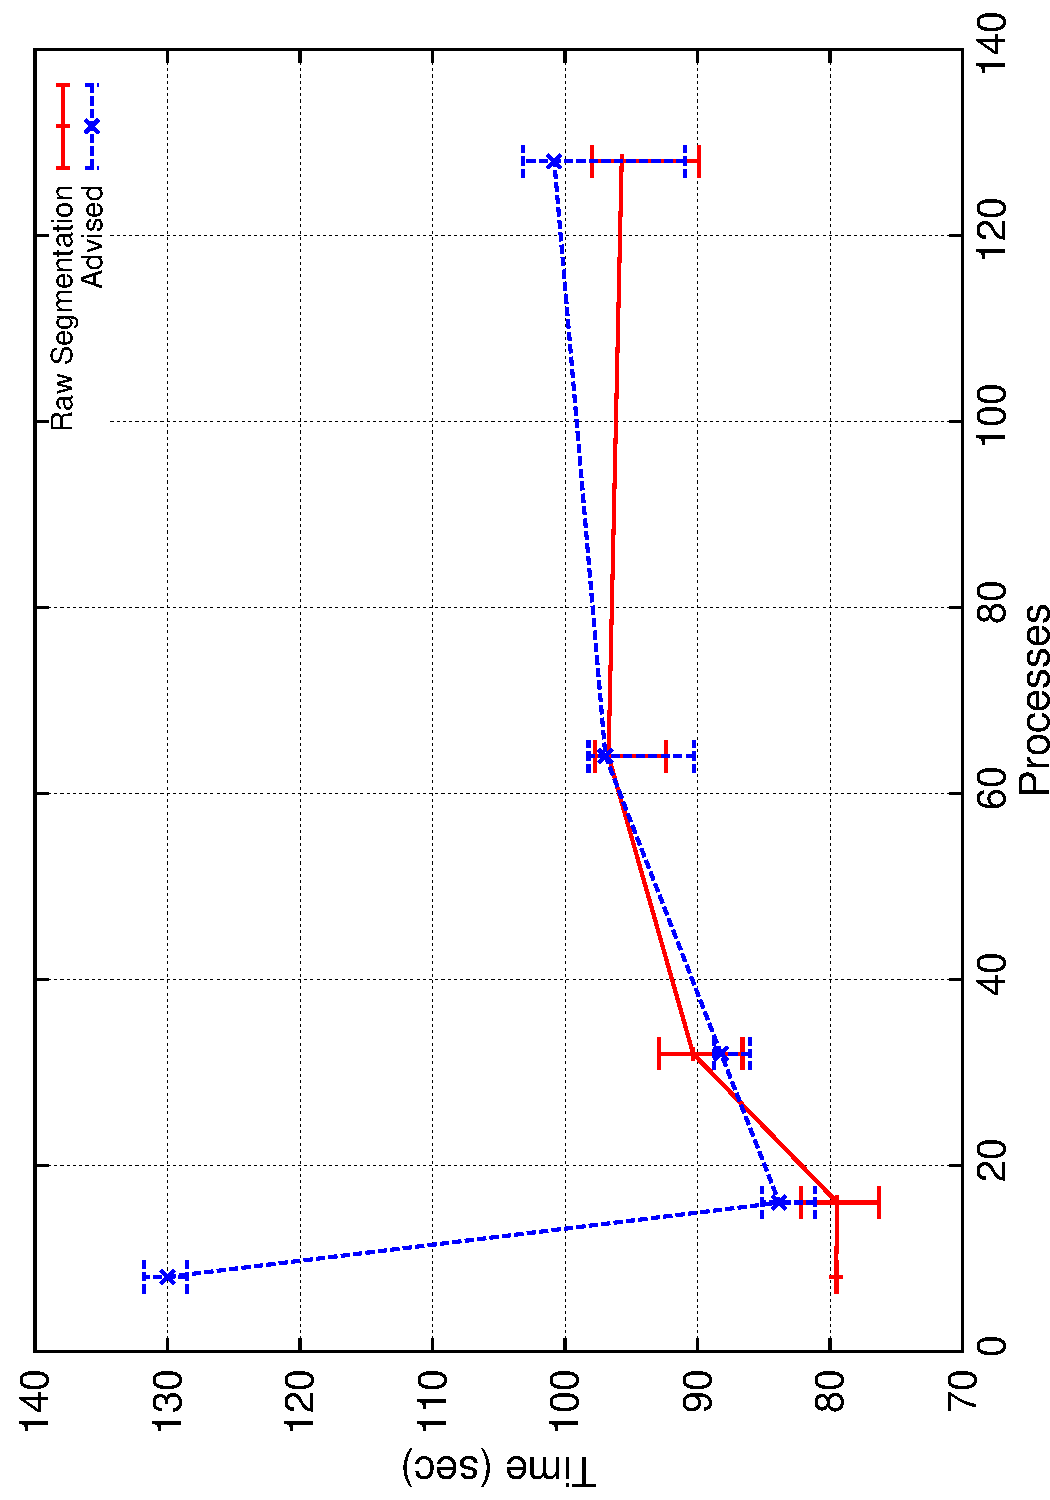
\includegraphics[angle=270,width=\linewidth]{images/io/lh-most}
  \caption{Raw segmentation strong scaling with and without explicit
  caching, on the second cluster.  Explicit single-block readahead
  makes little difference, especially at higher concurrency levels.}
  \label{fig:lh-most}
\end{figure}

Results from running on the second cluster are given in Figure
\ref{fig:lh-most}.  The HDF-backed NetCDF version could not be run on
this cluster due to a software incompatibility.

\begin{figure}
  \centering
  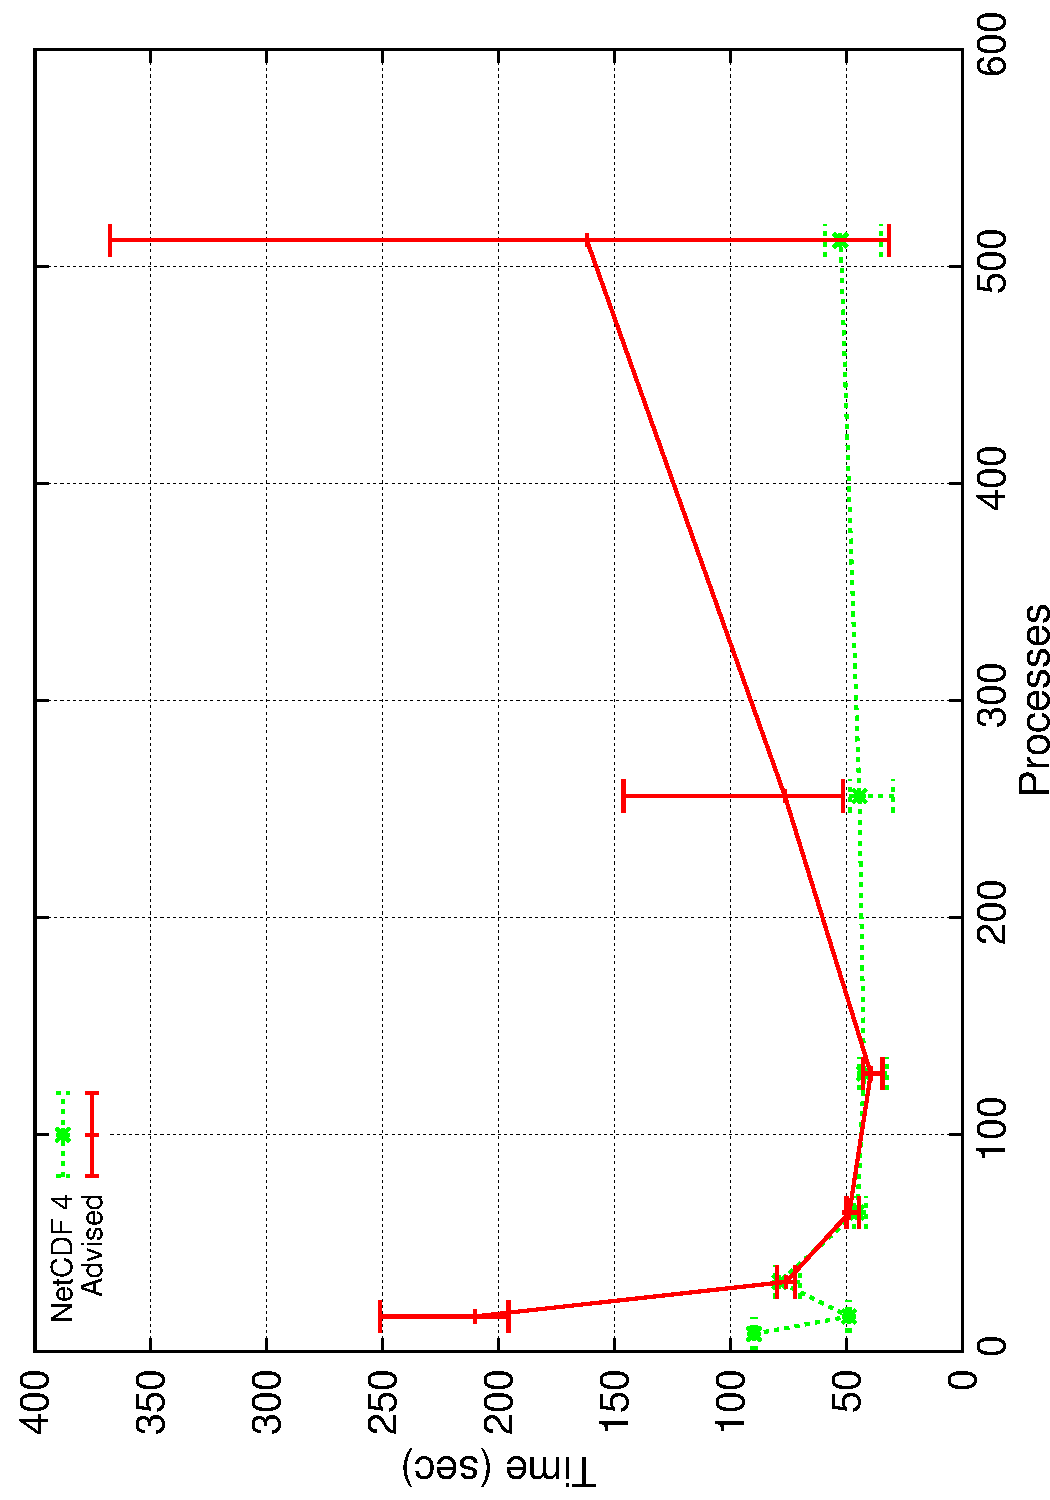
\includegraphics[angle=270,width=\linewidth]{images/io/jaguar-most}
  \caption{HDF-backed NetCDF and raw advised I/O method scaling on the
  third cluster.  Performance is largely the same at first, hinting
  that explicit readahead is likely too limited to be effective.  At
  higher levels of concurrency, our writes get very small, and the HDF
  backend is able to deal with the case much more effectively.}
  \label{fig:jaguar-most}
\end{figure}

Results from the third cluster are given in Figure
\ref{fig:jaguar-most}.  This machine is one of the largest scale
supercomputers we have access to, and so we performed runs at larger
levels of concurrency, although we did not utilize the entire cluster.
We only performed the `advised' version of our raw algorithm for this
cluster, as the simpler version gave essentially the same performance,
and compute time was harder to obtain for this machine.

%\subsection{ADIOS}
%
%ADIOS is unique in that it is not a file format alone, but rather a
%middleware suite that interfaces to a variety of backend methods for
%reading and writing data.  These methods include HDF5, NetCDF4 and
%ADIOS-only backends such as raw POSIX I/O and MPI-IO.  One of the
%promising features of this approach is that such a system could have
%rapid uptake of the results presented in work such as this.
%
%Unfortunately the current release at the time of publication (ADIOS
%1.2.1) does not yet support out-of-core data access.  For large-scale
%visualization applications, which commonly run on just a subset of the
%nodes utilized to produce simulation data in the first place, this is
%an essential feature.  We hope to include ADIOS results in a future
%study.

%\subsection{Custom Low-Level Data Access}
%
%This is a method we developed based on a series of experiments with
%different I/O methods on multiple machines.  The approach is rather
%simple: each process memory-maps a chunk of the large input data file,
%as well as the relevant portion of the output mask file.  Data are
%processed from the memory-map as-is.  The source is very simple, and
%contains now allocations other than those performed internally (for
%example, to initialize MPI).  As such, this version of the program
%required the least memory by a wide margin; the natural method of
%writing it was out-of-core.

% \begin{figure}
%  \centering
%  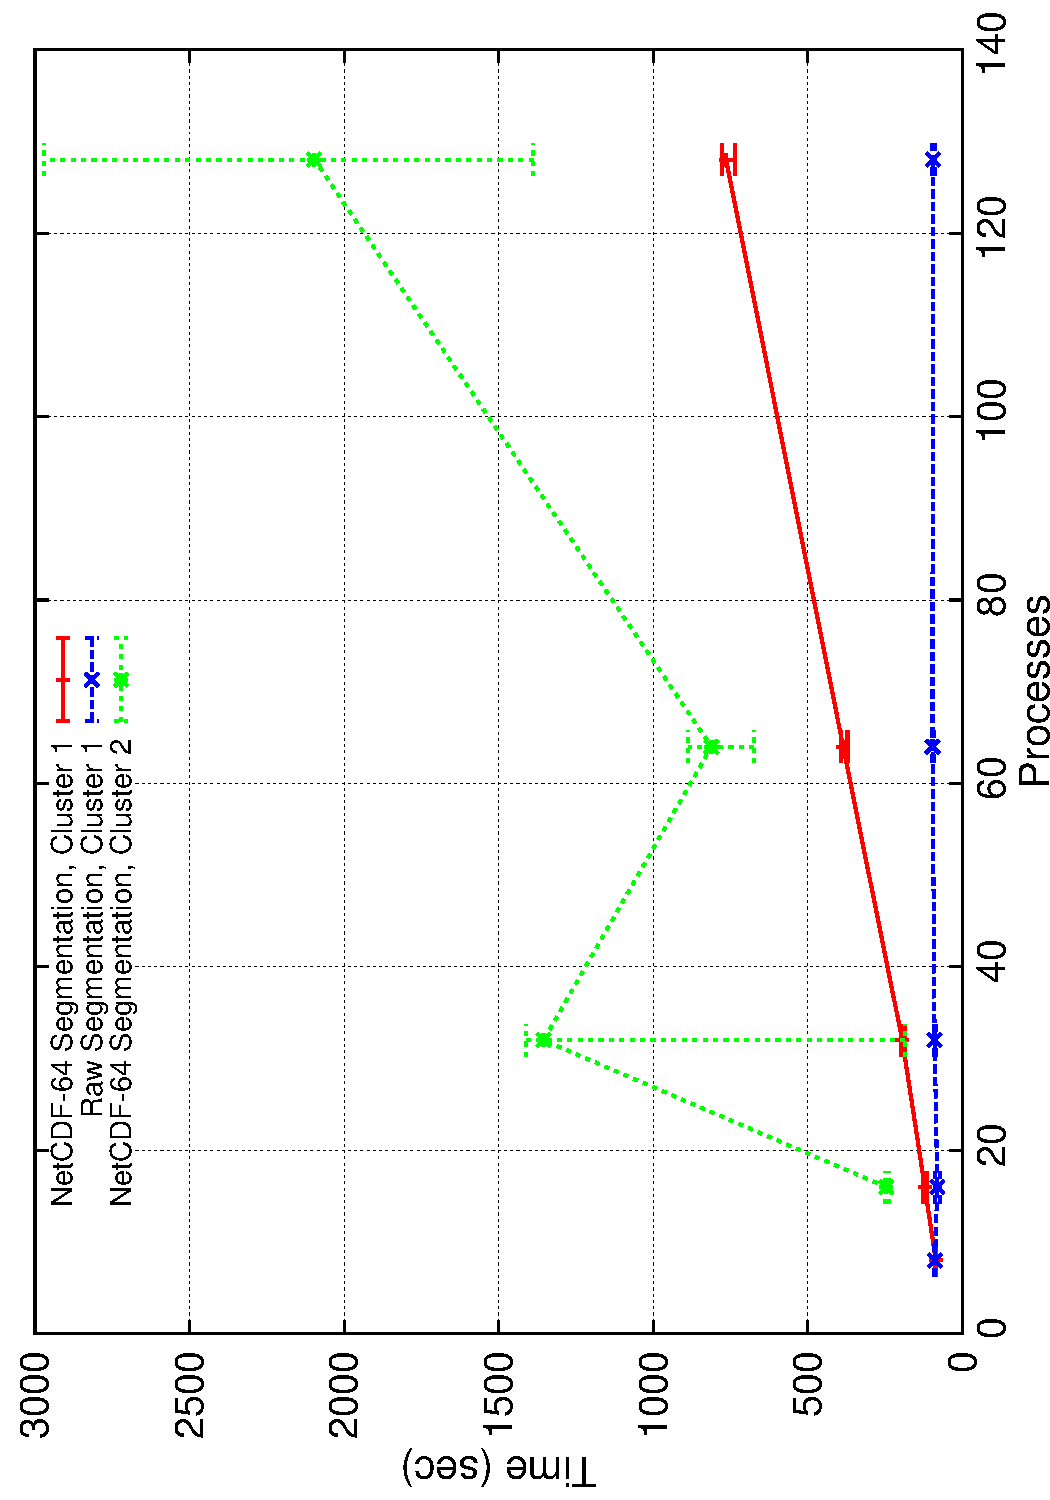
\includegraphics[angle=270,width=\linewidth]{images/io/lh-all}
%  \caption{
%  Strong scalability for a simple segmentation problem using NetCDF
%  `64bit offset' files and a custom I/O layer, on multiple clusters.
%  Error bars indicate minimum and maximum running times observed, per
%  process in the job.
%  {split things into two figures: one figure for Lens, one for Longhorn,
%  and another for Jaguar if I can fit runs in...}
%  }
%  \label{fig:lh-performance}
%\end{figure}

% Figure \ref{fig:lh-performance} shows the scalability of this program
% (`Raw Segmentation') alongside the results of the NetCDF4-backed
% files, run on the same cluster.  At scale, the performance appears
% to be flat.  However, we note that a closer look at the performance
% data indicates that performance increases up to 16 processors, and
% then begins to worsen.  This is due to our chosen problem; the
% thresholding segmentation is incredibly simple, and after 16 tasks we
% don't gain much of a benefit from more processors, as there simply is
% not enough work to go around.

% ``While we don't show the results, we ran the raw tests with a larger
% file, and confirmed that more processors brings the runtime down
% out to a larger number of processors, demonstrating that we just
% do not have enough work in our algorithm to scale this approach
% appropriately.  More complicated applications would see a greater
% benefit from this method.'' blah blah blah.


% This is still true, but the raw benchmark kicks so much ass that I
% don't think we need to go back and redo the NetCDF benchmarks &&
% ensure we're comparing apples-to-apples.
%\note{The raw I/O benchmark includes the `close' calls, but the
%(currently-running) NetCDF benchmarks you have going do not.  Probably
%want to go back and redo the NetCDF benchmarks to time that.}

\section{A Parallel File API}\label{sec:design}

In the work presented for this paper, as well as our previous
experience writing visualization and analysis programs targeting
supercomputers, we have noticed that the available I/O models presented
by the standard POSIX API is insufficient from both the producer and
consumer vantage points.  Implementers are not given enough information
about access patterns that applications are utilizing, which prevents
filesystems from optimizing for common tasks.  Library and application
developers, on the other hand, have no mechanism for communicating such
information.  The result is sub-par performance, with both parties
feeling like there is little that can be done.

For this reason, we present an API that:

\begin{itemize}
  \item models the way visualization and analysis application
  programmers think about their data,
  \item simplifies data access, and
  \item enables implementers to design effective filesystems.
\end{itemize}

A summary of the methods that the API provides is given in Table
\ref{tbl:api}.  Our primary goal with such an API is to encourage
application developers to structure their code in such a way that it
models a similar API, as it provides more information to lower levels.
At the same time, we hope middleware libraries and even kernel code
begin to offer APIs that allow application developers to provide this
kind of information.  In the end, there should be much more data about
the patterns and intent of data access that the application provides to
the levels that can make use of it.

\colorbox{lightgray}{\texttt{open\_range}} and
\colorbox{lightgray}{\texttt{close\_range}}; \verb!open! and \verb!close!
calls that work with byte ranges.
One of the issues that plagues I/O concurrency
at large scales is the inability to indicate which portion of data
a process intends to
access: each process only needs some subset of the overall data, but
cannot communicate this a priori to middleware or the runtime system.
To perform effectively in the majority of cases, caching, large stripe
sizes, and readahead must be employed by the I/O system.  However these
techniques create false sharing when byte ranges overlap.

A popular method to combat this problem is to create a single file per
process.  Since only one process accesses the file, it is clear to
the I/O subsystem that concurrent access is impossible.  While this
is effective at the small scale, at the highest levels of concurrency
the method becomes untenable due to overwhelming amounts of metadata:
listing all files in a directory would require making a hundred
thousand requests to a server.  Even if this were technically feasible,
it presents significant data management difficulties; it would be much
easier on users if we could contain results into a singular file.

Many analysis applications would be able to calculate the byte offset
they will need on a given process given just the total number of
processes and the dimensions of the dataset (or number of points in
a point mesh).  Visualization software may need to produce a spatial
hierarchy of the data, but again this can be done with relatively
little metadata.  By providing this information to the underlying
I/O subsystem up front, application developers can cleanly solve one
of the more difficult problems in defining distributed file systems:
distributed lock management.

It should be an error to specify a byte range beyond the file length
when opening a file for read-only access.  When used for write access,
this would be a viable method for extending the file's length.  All
offsets from a file opened in this manner are relative to the start of
the byte range.  Attempting to read beyond the end of the byte range
results in end-of-file.

If the API is made to work with existing file descriptors, the standard
\verb!close! call is the only API needed.  If this API returns a more
opaque type, an API-specific \verb!close! method will be required.

% \colorbox{lightgray}{\texttt{readdirv}}; a \verb!readdir! that accepts
% some type of globbing mechanism and communicates the result to all
% processes in a group.  Consider a visualization application asked to
% process a simulation's output.  The simulation generally created $N$
% files with a common prefix or suffix.  The visualization application
% must identify what that $N$ was and distribute those files among the
% $M$ processes it is presently running on.  The only ways to do this are
% to: 1) have each application \verb!readdir! and identify the files,
% or 2) \verb!readdir! on the root and broadcast the result.  (2) is
% superior, but it would be better if the machine that did the metadata
% lookup knew it had to broadcast the result.

\begin{table*}
  \centering
  \begin{tabular}{|c|l|}\hline
    \textbf{System call} & \textbf{Description}\\\hline
    \textit{open\_range} & open with an explicit range of accessible bytes.\\
    \textit{close\_range} & clean up resources associated with a
      buffer \\
    \textit{readanyv} & accept a set of blocks and returns when any one
      full block is available\\
    \textit{finished} & asynchronous flush; return immediately, but mark
      buffers as unused.\\\hline
  \end{tabular}
  \caption{Summary of proposed new APIs.}
  \label{tbl:api}
\end{table*}

\colorbox{lightgray}{\texttt{readanyv}}; a read that accepts a number
of blocks and returns one of them.  Many applications can identify
what data it will need using a small amount of metadata.  For the
segmentation application used in this work, for example, we could
compute that easily based only on the total amount of data and the
number of processes in the analysis job.  A volume renderer could
read just the world extents of each block and use that for a spatial
subdivision.  In short, it is common for an application to be able to
make progress given some small subset of its input, as long as each
subset is `complete' in some sense.  This interface allows an API
implementer to do \emph{intelligent} read-ahead; as demonstrated in our
test program, this can provide compelling performance advantages.

The API should return pointers; it should not accept previously
allocated buffers.  The gives the implementer freedom to manage
allocations, enabling flexibility in choices of underlying APIs.  For
example, memory-mapped files require page-aligned memory,
which is not provided by \verb!malloc! or \verb!new!, and is more
difficult to use at fixed addresses, as opposed to letting the kernel
choose the mapping.

\colorbox{lightgray}{\texttt{finished}}; an asynchronous flush
operation.  This indicates that the given file (or byte range within
the file, given \texttt{open\_range}) will no longer be used.  The
method returns prior to performing any I/O operations.  It is an
error to read from or write to the given file after performing
this operation.  It is an error to open the given file within the
same process without an intermediate \verb!close! operation.  An
implementation may detect these errors.  It is unspecified whether any
other process sees any modifications to the open file before a future
\verb!close! operation completes.

The intent is to allow a system to better manage its cache and write
throughput.  Should the system experience memory pressure, these cache
blocks are the best candidates to consider for flushing.  If the
network or host resources are currently busy, the system might delay
making the write request until a better time.  This would also allow
an implementation to avoid a `thundering herd' of disk write requests:
mitigated in a system such as Lustre, but a difficult problem in an
NFS-like environment.

It is important to note that, while this system interface was
explicitly developed to deal with the problems of distributed systems,
most calls could provide benefits for applications targeted to typical
workstations.  The issues are largely the same, though the stakes are
higher in a distributed system.  Furthermore, such a system would not
obviate the need for current infrastructure; not all file access can
be made to conform to this model, but the intent is that large scale
applications would be able to effectively utilize these APIs for their
primary I/O needs.

\section{Conclusions}\label{sec:conclusions}

We have presented performance characteristics of modern disks.
Utilizing that information, we evaluated a variety of APIs for
file access with large scale data by implementing the same program
using multiple backends.  Where APIs had options that may effect
performance, we experimented with those options to identify the set that
gave the best parallel performance on our chosen problem.  We evaluated
this program on multiple clusters, attempting to identify generalized
practices that application developers should follow to obtain superior
performance in the common case: where they have no control over where
their users will run the released code.

Variability in I/O performance, such as that depicted in Figure
\ref{fig:n64}, was considerably higher than we expected it to be.  In
some cases we observed a job taking twice as long to execute than it
did at another point in time.  This presents a difficult challenge
for interactive visualization and analysis applications, which should
provide the illusion of interactive response yet are highly susceptible
to such latency.  The results encourage the use of progressive or
multiresolution renderers that can be used to provide real-time
responses in the plausible event that the supercomputer cannot respond
quickly enough.

While the best performance was generally obtained by using operating
system APIs directly, we do not advocate developers use these directly
at this time.  Higher level libraries such as NetCDF, HDF5, and ADIOS
provide mechanisms for self-describing metadata and data attributes,
and can achieve similar performance with the proper configuration,
not to mention providing portability across a wider set of systems.
Instead of having every application developer familiarize themselves
with these to-the-metal APIs, our community should instead work towards
the goal of incorporating these ideas into higher level libraries.
However, some API changes, preferably to accomodate a model more like
the one
presented in Section \ref{sec:design}, could go a long way towards
getting users to write code that can be scaled much more easily.

For application developers, we present the following maxims for
obtaining the best I/O performance possible:

\begin{itemize}
  \item Stagger operations that read or write file metadata.
  \item Read or write in large chunks: 10 megabytes or more.
  \begin{itemize}
    \item This frees the developer from the requirement of
    identifying and implementing intelligent data layout schemes.
  \end{itemize}
  \item Use memory-mapped files whenever possible.
  \item If you can do more, unrelated work before \verb!close!-ing some
  file resource, do so.
  \item \emph{Always} check and report errors during \verb!close!.
\end{itemize}

\subsection{Limitations}\label{sec:issues}

Any study is subject to the limitations of that which can be tested, as
well as the time available to perform tests \textit{ad nauseum}.  This
study is no different, and suffers from at least the following barriers
and limitations on its conclusions.

The most serious is our chosen test application.  We have chosen to
implement a program that essentially maintains two small buffers
at any one time: a brick of the input file and an output brick.
In a real-world application, it would desirable to load as much
data as would fit in the current memory.  Furthermore, many current
applications are not intelligent enough to implement either method:
they employ strictly in-core algorithms.  Due to the memory struggle
between application heap allocations and the operating system's
filesystem caching, in-core applications clearly perform worse when the
heap memory required grows close to the available memory on a node.
%While out-of-core algorithms generally incur some amount of extra
%overhead, this is likely to be negligible.\cite{Fogal:2010:LargeData}
Finally, our application performs very little work on each input voxel;
this was done to emphasize I/O time, but is uncharacteristic of any
useful analysis program.
Therefore it is likely that the application presented here performs
better than real-world visualization and analysis applications.

A second issue, particularly with respect to the proposed API, is
the lack of thorough evaluation.  No applications have been written
to such an API.  We have implemented the API in user-space, but no
middleware or applications have as-yet been adapted to utilize the
model it presents.  Despite these shortcomings, we feel the approach is
well-informed based on our experiences here and in prior literature.

\section{Future Work}

The ADIOS library is unique in that it is not a file format alone,
but rather a middleware suite that interfaces to a variety of backend
methods for reading and writing data.  These methods include HDF5,
NetCDF4 and ADIOS-only backends such as raw POSIX I/O and MPI-IO.
Unfortunately the current release at the time of publication (ADIOS
1.2.1) does not yet support out-of-core data access.  For large scale
visualization and analysis applications, which commonly run on just a
subset of the nodes utilized to produce simulation data in the first
place, we judged this to be an essential feature.  We contacted the
development team and they agreed to look into out-of-core APIs for a
future release; we therefore hope to include ADIOS results in a future
study.

We would like to extend the methodologies used in this work to a larger
set of parallel algorithms.  In particular, algorithms that must
do considerably more per-voxel computation, and those that require
information from neighboring voxels.

% \subsection{Lustre Overview}
%
% Lustre (an almagmation of ``Linux'' and ``cluster'')
% is a distributed file system that is popular in mid-
% to high-end supercomputing facilities. The major claim
% is that Lustre is \emph{scalable}: administrators can
% add disks and new machines to a supercomputer without
% effecting the overall storage performance.
%
% Lustre filesystems are composed of: a single
% \textit{metadata~server} (MDS), many
% \textit{object~storage~targets} (OSTs), and any
% number of \textit{clients}. The filesystem presented
% to the user has standard POSIX access semantics,
% including advanced features such as locking. New
% machines with attached disks (OSTs) register with
% the MDS, and the MDS handles all indexing of data.
% In classic UNIX filesystem terminology, the MDS is
% essentially a collection of inodes and the OSTs store
% the actual file data.
%
% Knowledge of the filesystem's structure is useful in
% designing large-scale visualization applications. For
% example, consider what happens on an `open' of an
% existing file, depicted in Figure
% \ref{fig:lustre-open}.
%
% \begin{itemize}
%
%   \item The client contacts the MDS, sending a
%   filename and access information (read-only,
%   read-write, etc.).
%
%   \item The MDS responds with the basic inode
%   information, as well as a list of OST-to-indices
%   mappings for file locations (e.g. ``bytes 0-512 is
%   on OST hostA at index 6; bytes 512-1024 are on hostA
%   at index 7'').
%
%   \item In almost all cases, the client now contacts
%   the first (or first few) OSTs, trying to fill up a
%   readahead buffer.
%
% \end{itemize}
%
% Consider what happens when all processes in an MPI
% job open the same file: we get \verb!MPI_Comm_size!
% processors that all send a small message to the MDS,
% which must do a disk seek and read a few blocks
% before sending the data back. Then each of those
% \verb!MPI_Comm_size! contacts the OST with byte 0
% and asks for `cache size' bytes. In all likelihood,
% the MDS can get by with a single seek here, and it's
% transferring a small amount of data, so disk I/O time
% is negligible. However a large number of processes
% all requesting a network buffer takes its toll on an
% MDS. For example, by default the maximum number of
% connections a Linux kernel will have open at any one
% time is 128. If an MPI job tries to open a file on all
% processors, then a hundred thousand processes compete
% for 128 slots.
% \note{open-ro.c tests this case}
%
% The `cost' in the above situation is the summation
% of: N round-trips to the MDS, the time for the MDS to
% read the metadata, N small sends to request data from
% the OST[s], the time to read the data from the OSTs,
% and N times the transfer cost of the given data. More
% succinctly:
%
% % This logic needs to be fixed to account for striping.
%
% \begin{eqnarray*}
%   T & = & N \times T_{send->MDS} + \\
%     &&    1 \times T_{read,MDS} + \\
%     &&    N \times T_{send, metadata} + \\
%     &&    N \times T_{send->OST, request} + \\
%     &&    N \times T_{read, OST} + \\
%     &&    N \times T_{send, data}
% \end{eqnarray*}
%
% Since we consider metadata to be `small', we ignore
% transfer time when the MDS
% reads metadata. Thus $T_{read,MDS} = T_{seek}$, the
% time to seek to the appropriate metadata. We model
% network transfers as taking time $M + nB$, where $M$
% is a constant message setup cost and $B$ is a per-byte
% cost, and we use similar simplifications here,
% discounting per-byte overhead for metadata on the
% basis that $nb << M$. Using those transformations,
% our costs become clearer:
% \begin{eqnarray*}
%   T &=& {} + N \times M  \\
%     &&  {} + T_{seek, MDS} \\
%     &&  {} + N \times M \\
%     &&  {} + N \times M \\
%     &&  {} + N \times (T_{seek} + T_{rotational} + T_{transfer}) \\
%     &&  {} + N \times (M + nB)
% \end{eqnarray*}
%
% We consider network performance numbers as given in
% \cite{Rodrigues:FastSockets:1997} \TODO{something newer?}
% Regardless, per-message and per-byte
% overhead is measured in tenths of microseconds; a
% message costs about a third of a microsecond, and a
% byte costs approximately 0.2 microseconds. Therefore
% at just over 4k bytes the per-byte overhead adds up to
% about a millisecond; we can send 37,000 bytes in the
% time it takes to seek on an average disk.  This gives us a function for the
% time taken
% \begin{eqnarray*}
%   T(N, b) &=& {} + 3(N \times 0.3 \mu{}s) \\
%           &&  {} + 9 ms \\
%           &&  {} + N \times (9ms + 4.2ms + b/102400) \\
%           &&  {} + N \times (0.3 \mu{}s + 0.2 b \times 1024)
% \end{eqnarray*}
%
% where $N$ is of course of the number of processes
% in the system and $b$ is the number of bytes to
% read, in kilobytes. The function makes the same disk
% assumptions that we did earlier.
%
% \begin{figure}[Htb]
%   \centering
%   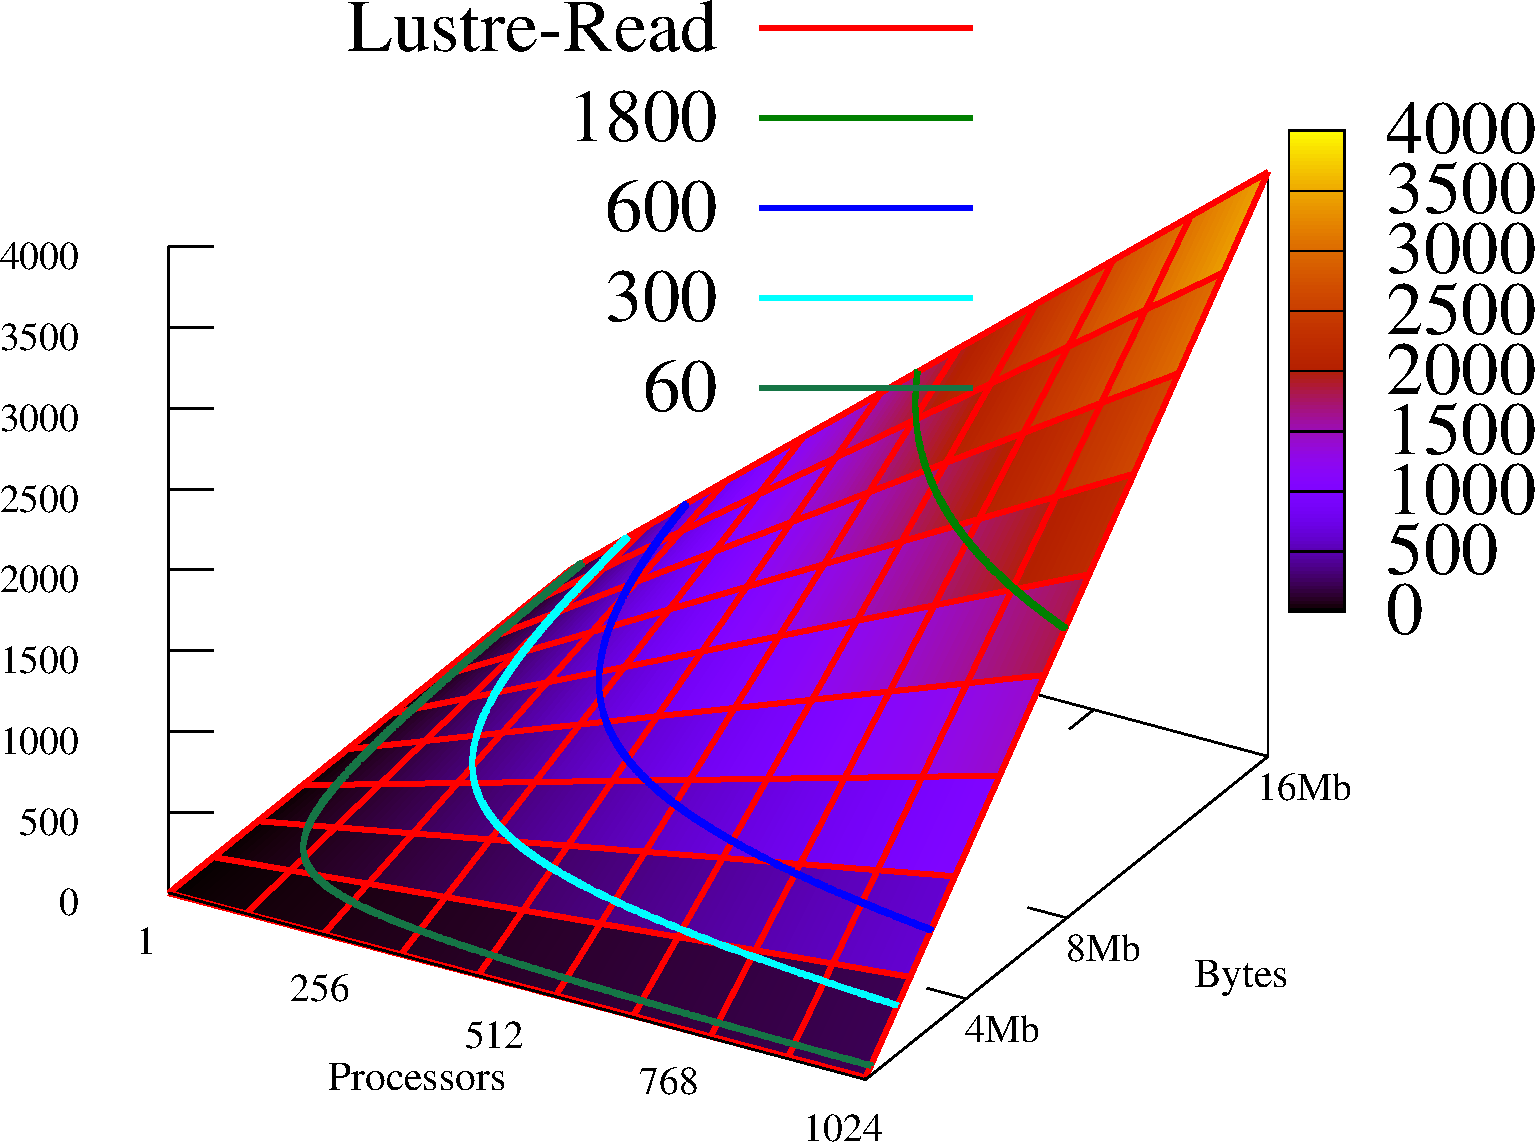
\includegraphics[width=\linewidth]{images/io/lustre-read}
%   \caption{Best case read performance with Lustre.}
%   \label{fig:lustre-read}
% \end{figure}

% Compare this situation to application-level input: the
% program could easily be written to have process 0 open
% and read the desired data, and then send out the data
% to the processes that need it.  This would incur:
% \begin{eqnarray*}
%   T(N, b) &=& {} + 0.6 \mu{}s + (N \times 0.3 \mu{}s) \\
%           &&  {} + 9ms \\
%           &&  {} + (9ms + 4.2ms + (N \times b/102400)) \\
%           &&  {} + 2N \times (0.3 \mu{}s + 0.2 b \times 1024)
% \end{eqnarray*}
%
% Now only one process contacts the MDS; accordingly,
% the request and return are only paid once. Process 0
% still must send N requests for data, however. Seeking
% on the MDS is unchanged: we only looked for one file
% in the first place anyway. We avoid all but one of the
% seek costs on the OST
% BLAH -- the above is wrong, the file will be striped
% across multiple OSTs. Need to fix the case before
% this too.

% \note{Verified on Lens and Longhorn: the default
% stripe count in Lustre is 4, and the default stripe
% size is 1 megabyte. This is probably pretty terrible
% for performance. We should incorporate this info into
% the text, somehow...}


\chapter{Freeprocessing}
\label{chp:freeprocessing}
\newcommand{\freeprocessing}[0]{\textit{Free}processing}
\newcommand{\freeprocessor}[0]{\textit{free}processor}
\newcommand{\nullset}[0]{$\varnothing$}
\newcommand{\insitu}[0]{\textit{in situ}}

%\newcommand{\nullset}[0]{$\emptyset$}
\definecolor{lightgray}{gray}{0.85}

\textit{In situ} visualization has become a popular method for avoiding
the slowest component of many visualization pipelines: reading data
from disk.  Most previous \insitu{} work has focused on achieving
visualization scalability on par with simulation codes, or on the data
movement concerns that become prevalent at extreme scales.
In this work, we consider \insitu{} analysis with respect to ease of
use and programmability.  We describe an abstraction that
opens up new applications for \insitu{} visualization, and demonstrate
that this abstraction and an expanded set of use cases can be realized
without a performance cost.

\section{Introduction and related work}

% The growing size of simulation outputs
% - sims producing much more data
% - too slow to load in for vis
% -> rise of in situ
% - other approaches as well
%   - data staging (io nodes)
%     - enables asynch
%   - co-analysis
%   - acceleration of io (vishwanath)

The growing size of simulation data and the problems this poses
for subsequent analysis pipelines has driven simulation authors to
integrate visualization and analysis tasks into the simulation
itself~\cite{Childs:2013:ChallengesVis}.  The primary advantage of
this approach is to perform operations on data while they are still in
memory, rather than forcing them through disk, thereby eliminating the
most expensive component of the majority of visualization and analysis
pipelines.

Scientists and engineers have developed many different approaches
to \insitu{}.  DART uses RDMA to stage data from supercomputer to
potentially separate analysis-focused
resources~\cite{Docan:2010:DART}, and a system performs computations on
the data as they are in transit from one resource to
another~\cite{Moreland:2011:InTransit}.  The dominant approach is
to use the same supercomputer that is running the simulation for
visualization, though potentially on just a subset of cores, in the
manner of
Damaris/Viz~\cite{Dorier:2013:Damaris}.  Damaris/Viz can provide a
wealth of visualization and analysis opportunities due to its ability
to act as a
front end to both VisIt's~\cite{Childs:2012:VisIt}
\texttt{libsim}~\cite{Whitlock:2011:Libsim} as well as ParaView's
Catalyst~\cite{Fabian:2011:Catalyst, CatalystUserGuide}.  Biddiscombe
et al. proposed an HDF5-based driver that forwards the data from HDF5
calls to ParaView~\cite{Biddiscombe:2011:HDF5Steering}; we give an
example of our system implementing similar functionality in
\S~\ref{sec:enzo-example}.  Abbasi et al. introduce DataStager,
a system for streaming data to staging nodes and demonstrate a
performance benefit by asynchronously streaming multiple buffers at one
time~\cite{Abbasi:2009:DataStager}. \textit{In situ} libraries can also
be used to improve the performance of simulation
code~\cite{Vishwanath:2011:Leadership}.

Most work focuses on extreme-scale performance with less regard for the
effort required in integrating simulation and visualization software,
whereas we focus on the latter concern.  Notably, however, Abbasi et
al. extend their previous work with a JIT compiler that allows users to
customize data coming through
ADIOS~\cite{Lofstead:2008:ADIOS} using snippets of code written in a
subset of
C~\cite{Abbasi:2011:JITStaging}.  Zheng et al. modify OpenMP runtimes,
an approach that shares our mentality of working within the
constraints of existing
infrastructure~\cite{Zheng:2013:GoldRush}.  Others have tightly
integrated simulation with visualization to allow steering, but these
generally come at high integration costs~\cite{Lesage:2012:FlowSitu,
Ament:2011:Steering}.

% Freeprocessing can implement that idea for specific domains; the main
% differences are that binary instrumentation can do this with 1) any
% software and 2) for any writes, not just writes that go through a
% specific library.

% - existing solutions leave potential users behind
%   - difficulty / lack of desire for middleware
%   - maybe file i/o isn't synchronous (e.g. adios requires synchronous opens)
%   - perceived benefit (correct or no) too low
%   - existing infrastructure with custom domains

Existing solutions leave a potentially large segment of the user
community behind.  Most previous work has integrated or presupposed
integration with particular libraries for performing I/O operations,
and no such library has achieved universal adoption.
Yu et al. note the tight collaboration required
for a fruitful integration~\cite{Yu:2010:Combustion}.  Reasons for
not adopting I/O middleware are varied: the difficulty in integrating
the library with local tools, perceived lack of benefit, lack of
support for existing infrastructure with home-grown formats, or issues
conforming to required interfaces, such as synchronous `open' calls.

%   - simple problem/code: no need for middleware
%     - all the serial sims out there
%     - matlab / octave?
%   - middleware doesn't make any sense: HDF5 in openssh?
%   - additional libraries complicate code: must evolve together
%   - diverse use case
%     - non-simulation uses: provenance? instrument all launched programs

Moreover, the focus of modern I/O middleware specifically on
simulations at the extreme scale leaves a long tail of potential
\insitu{} uses behind.  The set of simulation authors focused on
creating exascale-capable simulations is a small subset of all
simulation authors.  A large set does not even dream of petascale;
and even larger are those who would barely know how to exploit a
terascale-capable solver for their science.  The distribution gets
larger and more diverse as one moves out to lower scalability levels.

At the opposite end of `extreme scalability' uses for \insitu{}, one
may find a number of heretofore ignored applications.  There is no
reason to limit the \insitu{} idea to parallel code running on a
supercomputer, for example.  Analysis routines embedded into the fabric
of network transfer operations would be a boon to distributed research
groups (and
the success of tools such as Globus~\cite{Foster:2011:Globus} speaks
to the multitudes of domains faced with this problem).  Those
writing simulations in MATLAB\textsuperscript{{\tiny \textregistered{}}} might
also benefit from precanned visualization tasks that occur concurrently
with their simulation, yet the closed source nature of the product
makes the prospect of integrating I/O middleware improbable at best.

The currently-dominant middleware approach to \insitu{} requires
significant effort.  It is reasonable for simulation authors to spend a
week integrating and retooling their code to achieve
thousand-way concurrent \insitu{} visualization, but this level of
investment is unreasonable to users who simply wants to compute a
data range on their files as they move across the country.  The cliff
between `nothing' and
a `100\%' solution for \insitu{} visualization with
existing middleware solutions is too high to appease such diverse
use cases.  Worse, the model is unworkable in some situations;
it is doubtful that the OpenSSH maintainers would accept patches
incorporating
ParaView's Catalyst into \texttt{sftp}, for example.

\textit{Free}processing is an abstraction of previous work.  Using
it, one can implement classical \insitu{} visualization and analysis,
computation or data reduction via staging nodes, unique instrumentation
such as gathering power consumption information
dynamically~\cite{Gamell:2013:InSituPower}, or a number of novel
`processing while moving data' ideas.  This processing can be
synchronous or asynchronous depending on the needs and desires of the
user.  Developers of a \freeprocessor{} can connect it to existing
visualization tools such as VisIt's \texttt{libsim} or ParaView's
Catalyst, implement their own analysis routines, and even push data
into another language such as Python, all without data
copying---\emph{or} with data copying, should those semantics be
preferable.  The general
nature of \freeprocessing{} not only allows one to implement the
diverse domains of previous work, but also allows novel use cases.
Specifically, we contribute:

% - freeprocessing is an abstraction of previous work
%   - can copy data or work with it in the same address space
%   - can be synchronous or asynchronous with simulation code
%   - can implement classical in situ
%   - can implement the `in transit' mode of DataStager
%   - can implement `DART'
%   - can implement visualization during data transfer
%   - can implement data conversion
%   - can forward data to ParaView's catalyst for tool-specific in situ
%   - can implement i/o acceleration (delayed closes?)
%   - can implement special provenance tracker

\begin{itemize}

  \item a new method for inserting data processing code into I/O
  operations;
%, including demonstrations that previous work can be
%  implemented within it;

  \item the generalization of \insitu{} ideas to heretofore unexplored
  domains, such as visualization during network transfer;

  \item greatly increased programmability for \insitu{} ideas, making
  them applicable with considerably less effort;

  \item a sample implementation that demonstrates all of these ideas in
  real-world cases.

\end{itemize}

The rest of this paper is organized as follows.  First, we explain the
technical underpinnings of how the program works.  In
\S~\ref{sec:classical} we demonstrate
\freeprocessing{} in some classical environments and show that there
is almost no overhead.  We demonstrate some novel uses
before we conclude and note limitations as well as future work in
\S~\ref{sec:conclusion}.

% \section{Previous work}
%
% Others have proposed solutions to the problems within \insitu{}
% parallel visualization and analysis.

% Gamell et al. detail the power requirements of a prototypical \insitu{}
% workflow~\cite{Gamell:2013:InSituPower}.  DART uses RDMA to stage data
% from the supercomputer to potentially-separate
% analysis-focused resources~\cite{Docan:2010:DART}.  Continuing this
% idea of utilizing a smaller set of nodes for visualization and
% analysis, Damaris/Viz adds visualization to an I/O-oriented framework
% at demonstrably low
% overheads~\cite{Dorier:2013:Damaris}.  It can act as a frontend to
% both VisIt's~\cite{Childs:2012:VisIt}
% \texttt{libsim}~\cite{Whitlock:2011:Libsim} as well as
% ParaView's Catalyst~\cite{Fabian:2011:Catalyst}.  Biddiscombe et al.
% proposed an HDF5-based driver which forwards the data from HDF5 calls
% to ParaView~\cite{Biddiscombe:2011:HDF5Steering};
% \S~\ref{sec:enzo-example} gives an example of our system implementing
% similar functionality.

% In doing so, we make simulation software easier to instrument, make it
% much simpler to plug-in alternate visualization and analysis tools, and
% enable uses of `\insitu' ideas in novel environments.

% [in contrast to GoldRush], our method 1) requires no maintenance for
% updating runtimes, 2) works even if a simulation does not utilize
% OpenMP, and 3) does not have the initial cost of porting to a new
% runtime.

% \section{Structure of a simulation}
% \label{sec:structure}
%
% The common method to enable \insitu{} visualization in an existing
% simulation is to make a coupling library available to simulation
% software, change the simulation source code to call the new API, and
% recompile the simulation code, additionally linking the visualization
% tool as a library.  This is a significant investment: while the
% multiple simulations which use it can amortize the development costs
% of the coupling library, instrumenting the simulation source code
% is necessarily a per-simulation cost.  Furthermore, visualization
% software is typically multiple orders of magnitude more complicated
% to build than the simulation code which then utilizes it.  This
% can be a large barrier, particularly when simulation authors are
% not well-versed in the arcane lore of large-scale C++ software
% development.
%
% One of the most complicated components of this process is in
% modifying the simulation code: it must push the data over to the
% visualization software, and it must relinquish and regain control
% periodically to allow the visualization tool to produce its output.
% The decision of where to insert these code changes can be difficult
% for a simulation author, especially when the simulation scales better
% than the visualization tool.  Insertion of this `glue' code is also
% problematic if there are cases in which running the visualization
% tool is undesirable or even impossible---for example, when the
% simulation tool supports a particular esoteric architecture that the
% visualization tool does not.  Furthermore, there can be an impedance
% mismatch between the two tools, for example if the visualization tool
% requires both a grid and associated data in a single call, but the
% simulation does not colocate this information in time (instructions)
% or space (memory).
%
% Yet all simulations must fulfill the contract of writing and
% describing its data, at some point.  To this end, we have analyzed
% a number of simulation packages to identify their overall
% structure---essentially the operations in their outermost loops.

\section{Instrumentation}
\label{sec:instrumentation}

\begin{figure*}
  \centering
  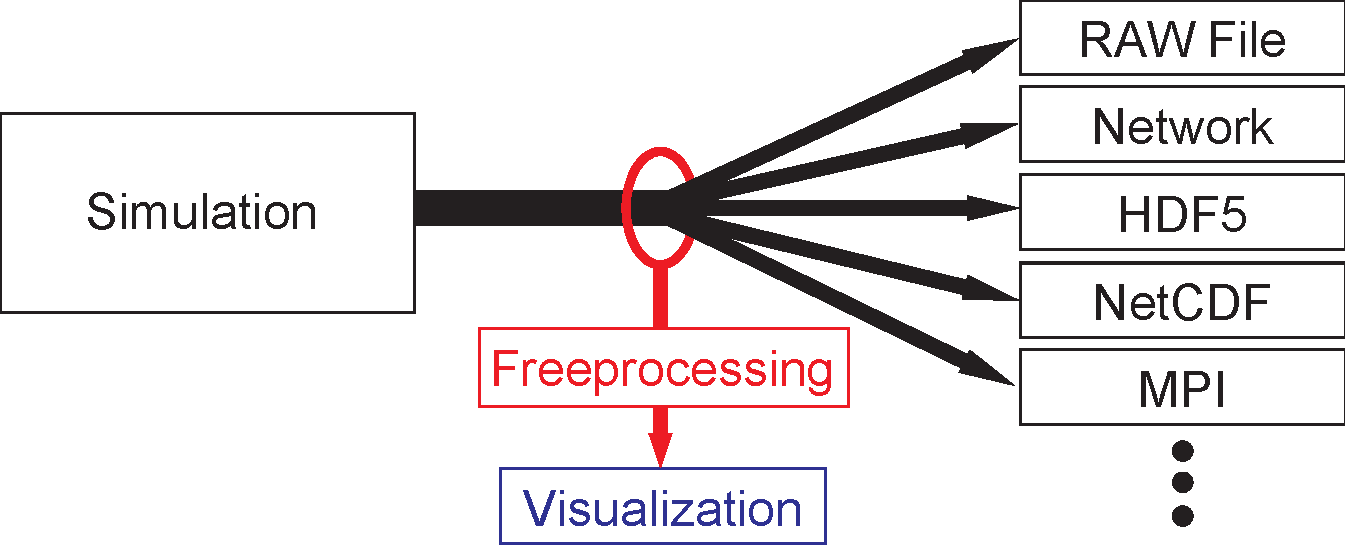
\includegraphics[width=0.95\linewidth]{images/fp/fp}
  \caption{\textit{Free}processing works like a vampire tap on the data
  coming out of a simulation.  Without changes to a program's source
  code, we can intercept the data as it goes to the IO library and
  inject visualization and analysis tasks.}
  \label{fig:interchange}
\end{figure*}

Previous \insitu{} solutions have relied on the simulation author
explicitly invoking the visualization tool, or the simulation using a
custom library for I/O, which is then repurposed for analysis.  In this
work we demonstrate that there is little need for
either; every simulation produces output already, an \insitu{} tool
just needs to tap into that output.

Our symbiont uses binary instrumentation to realize that tap. We take
unmodified simulation binaries and imbue them with the ability to
perform visualization and analysis tasks.  In doing so, we remove a
potentially
complicated component of \insitu{}: modifying the program to work with
the visualization or analysis tool.  Notably, this approach
enables simulation software to produce \insitu{} visualizations even
when the source code of the simulation is unavailable.  Furthermore, as
the symbiont interposes these functions during load time, a user need
only change the invocation of the program to enable or disable these
features.

%%%% ---- %%%%%

The method we use is to redefine some of the standard I/O functions, in
a similar manner to the way the
GLuRay or Chromium systems operate~\cite{Brownlee:2012:GLuRay,
Humphreys:2002:Chromium}.  These methods rely on features available in
runtime dynamic linkers to replace any function implemented within a
library at load time.  The overridden entry points form what we call
the `symbiont', the core of
\freeprocessing{}. The symbiont's purpose is to conditionally forward
data to a
\freeprocessor{}---a loadable module that implements the
desired \insitu{} computation---in addition to fulfilling the
function's original duties.  Separating the instrumentation itself and
the \freeprocessor{} allows users to develop processing elements
without knowledge of binary instrumentation.

The set of intercepted functions is different depending on the I/O
interface that the
simulation uses, as shown in Figure~\ref{fig:interchange}.  For the C
language, these functions are those of the POSIX
IO layer, such as \texttt{open(2)} and \texttt{write(2)}.  In Fortran
these calls are implementation-specific, and C++ implements I/O
differently, but on POSIX-compliant systems all such implementations
are ultimately layered on top of the POSIX I/O interface.  We also
introduce interposition for higher-level functions, such as those that
comprise MPI File I/O, and a subset of calls from the HDF5 family.
Using this interposition, what the simulation believes is a standard
`write' operation actually calls in to our symbiont.

\subsection{Data semantics}

Function interposition for higher-level functions from libraries such
as HDF5 and NetCDF provide an important benefit: data semantics.  As
these formats are self-describing, there is enough information in just
the stream of function calls to identify data properties---in contrast
to raw POSIX I/O functions, which provide little more than an abstract
buffer.  The symbiont forwards any available data semantics from the
interposed library functions to the
\freeprocessor{}.

However, in contrast to previous work, \freeprocessing{} will also
willingly forward data without knowledge of any underlying semantics.
A \freeprocessor{} can also ignore metadata simply by not implementing
the methods that interpret those messages.  This distinction is
important, as it both enables \freeprocessing{} to function in a larger
set of scenarios, as well as increases the flexibility of the system.
Presumably a \freeprocessor{} would then obtain this information from
some external source.  We view allowing semantic-less data transfer
similar to using `dangerous' constructs in a programming language, such
as casts in C.  While these constructs are generally
frowned upon, with restrained application they can be a powerful and
thereby useful tool.

% We view it much in the same way as a cast in C: it is dangerous,
% unwieldy, and a source of bugs, so one should never program this
% way---unless, of course, you have to, or it would be really inefficient
% otherwise, or it is an
% hour before a meeting and you \emph{need} this result, or these data
% really \emph{will always} be $32^3$, or ...

\subsection{Data semantics}

Meta-information concerning data semantics are required, and are
only available through \freeprocessing{} in limited cases.  While we
consider such concerns beyond the scope of this work, they need to be
provided for the demonstration of the technique.  The general nature of
\freeprocessing{} allows any number of solutions: the problem is no
different than understanding arbitrary binary data read from a file.
One of the solutions we have found works well is a simple text file
in the style of Damaris/Viz or ADIOS~\cite{Dorier:2013:Damaris,
Lofstead:2008:ADIOS}.  An example of one such configuration
is given in Listing~\ref{lst:jscfg}.  However, it is important to
note that this configuration is external to \freeprocessing{}
itself.  The symbiont does not contain this parsing and metadata
acquisition code; the `user
code'---\freeprocessor{}s---implements this only if they desire.

%We provide code which the user can drop into their code for this
%purpose, but there is no library a user must link against to implement
%a
%\freeprocessor{}.  Not forcing a metadata mechanism is useful, for
%example, in the instrumentation of PsiPhi (\S~\ref{sec:psiphi}), which
%already describes its output in a custom manner.  In previous work, such
%metadata would need to be duplicated in the \insitu{} tool's
%configuration.

\begin{minipage}{\linewidth}
\lstinputlisting[label=lst:jscfg,caption=JSON configuration file used
for a Silo conversion \freeprocessor{}.  Variants that do not require
the repeated \texttt{"i"}s are possible\textrm{,} but lack the desirable
property of strict adherence to the JSON specification.]{silo.json}
\vspace{-0.01em}
\end{minipage}

\freeprocessing{} itself does not endorse any specific method for
obtaining data semantics, in the same way that the C file I/O routines
do not endorse a specific encoding for metadata on binary streams.

%We note, however, that \freeprocessing{} leaves issues related to data
%semantics open.  There are a plethora of methods to communicate this
%information out-of-band, all of which are possible to implement with
%\freeprocessing.

\subsection{Defining \freeprocessor{}s}

The module interface for a \freeprocessor{} is simple.  The system
exposes a stream processing model.  Data are input to the processor,
utilized (or ignored), and thereafter unavailable.  This interface is
in principle the same model as GLSL, OpenCL, and CUDA expose, though we do not
currently impose the same restrictions.  A \freeprocessor{} is free to
implement a cache and process data in a more traditional manner, for
example.

Listing~\ref{lst:interface} shows the \freeprocessor{} interface.
The symbiont calls \texttt{Init} when a file is first accessed; some of
our \freeprocessor{}s initialize internal resources here.  The
\texttt{filename} parameter allows the processor to provide different
behavior should the simulation output multiple file formats.  The
\texttt{buffer} and \texttt{n} parameters are the data and its size in
bytes.  If the required information is available, the symbiont will call
\texttt{Metadata} immediately before a write, communicating the
characteristics for the impending data.  Likewise,
\texttt{finish} cleans up
any per-file resources.  Finally, the \texttt{create} function
implements a `virtual constructor' to create the processor.
All functions sans \texttt{create} are optional; if a
\freeprocessor{} has no need for metadata, for example, it simply does
not implement the corresponding function.

\begin{minipage}{\linewidth}
\lstinputlisting[language=C++,label=lst:interface,caption=Base class for a
\freeprocessor{}.]{interface.c}
\vspace{-0.01em}
\end{minipage}

\subsubsection{Configuration}

The symbiont reads a configuration file that describes
which \freeprocessor{}
to execute.  Any library that satisfies the interface given in
Table~\ref{lst:interface} is a valid \freeprocessor{}.  It is important
to note that the operations share the semantics of the simulation code.
For example, if a parallel simulation performs only collective writes
for a given file, then it is appropriate to perform
collective operations in the \freeprocessor{}'s \texttt{Stream} call.

It is common for a simulation to produce a large set of output
files.  Furthermore, MPI runtimes frequently open a number of files
to configure their environment, and all these files are `seen' by the
symbiont.  It is therefore necessary to provide a number of filtering
options.  Some of these are built in, such as ignoring files that
are opened for read-only access.  Others the user specifies in the
configuration file for the symbiont.  The specification uses a match
expression for the filenames, so the user can further limit where
instrumentation will occur.  These match expressions provide a more
convenient mechanism to uniquely connect processing elements to
streams, but the
assignment could also be done by the \freeprocessor{} implementation.

\subsubsection{Python}
\label{sec:python}

Developers may also implement \freeprocessor{}s in Python.  We provide a simple
\freeprocessor{} that embeds the Python interpreter and exports data
and needed metadata.  Most notably, it creates the
`\texttt{stream}' variable: a NumPy array for the data currently being
written.  Exposing the array to Python does not require a copy; the
simulation data shares the memory with the Python runtime.  Should
the Python script attempt any write operation on the data, a copy is
transparently made inside the Python runtime, which is then managed via
Python's garbage collector.  We allow only one of the simulation or the
Python tool to run at any given time.

The Python script is otherwise indistinguishable from standard Python
code; the symbiont imposes no restrictions beyond the unique source of
data.  Communication via, e.g., MPI4Py is even possible, provided the
simulation utilizes synchronous writes.
In \S~\ref{sec:enzo-example} we demonstrate this method by connecting
\freeprocessing{} with the \texttt{yt}
visualization tool~\cite{Turk:2010:yt}.

% It is worth noting that choosing to utilize Python somewhat complicates
% the use of \freeprocessing{}.  In particular, search paths for Python
% libraries---and shared libraries they link against---must be carefully
% configured so that they propagate into the more limited environment of
% the simulation code.  This is no different than the situation with, for
% example, ParaView's Catalyst; their documentation notes the same
% tradeoff~\cite{CatalystUserGuide}.

\section{Classical in situ}
\label{sec:classical}

\freeprocessing{} can implement a number of \insitu{} ideas,
including the traditional use case of \textit{in situ}: visualization
and analysis during a simulation run.  In this section, we detail how
the
corresponding \freeprocessor{}s for a few simulation codes operate, and
demonstrate that the overhead of the method is negligible.

\subsection{PsiPhi}
\label{sec:psiphi}

\begin{figure}
  \centering
  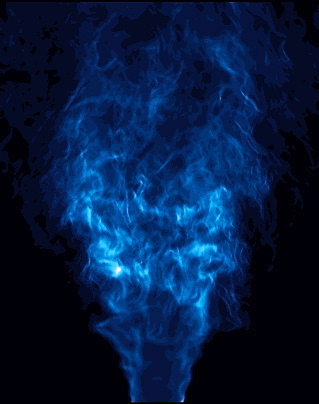
\includegraphics[width=0.48\linewidth]{images/fp/PsiPhi-vring.png}
  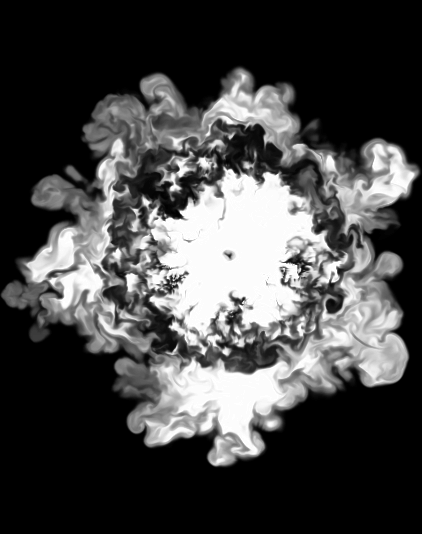
\includegraphics[width=0.48\linewidth]{images/fp/PsiPhi-slice.png}
  \caption{Sample \textit{in situ} visualizations of the Cambridge
  stratified flame produced by the PsiPhi code.}
  \label{fig:PsiPhi}
\end{figure}

PsiPhi is a Fortan95/2003-based CFD-solver that focuses on Large Eddy
Simulation (LES) of flows that include combustion and other types of
chemical reactions.  The simulation discretizes the governing equations
of mass, momentum, and species concentration on a cartesian grid via
the finite volume method.  Second-order schemes discretize the domain,
and an explicit third-order low storage Runge-Kutta scheme advances
the solution.  The immersed boundary (IB) technique handles diverse
geometries in a computationally efficient manner.  Besides the solution
of the mentioned transport equations in an Eulerian formulation, the
code is able to solve the equations of motion for Lagrangian particles.
A combination of Lagrangian particles and immersed boundaries describes
moving objects.  The code is modular, easy to extend and maintain, and
highly portable to different machines.  PsiPhi parallelizes via the
distributed-memory paradigm, using MPI.

% would be good if \cite{Franchetti2013PCI} fit in this list as well...

PsiPhi simulates highly-resolved simulations of reactive flows, e.g.,
premixed, non-premixed and stratified combustion, coal and biomass
combustion, liquid spray combustion, and nanoparticle
synthesis~\cite{Pettit2011PCI, Ma2013CTM, CavalloMarincola2013PCI}.
The software has scaled to thousands of cores on Top500 machines such
as SuperMUC and JUQUEEN.  Recent tests with the program have shown
that the output of the computational results becomes a performance
bottleneck when moving up to an even higher number of cores.

There are three types of intermediate outputs in the PsiPhi simulation.
The first
are actually custom-developed \textit{in situ} visualizations: slice
outputs and volume renderings.  The simulation writes out these
visualizations in custom ASCII-based formats every $n$ time steps, with
typical values of $n$ in
between 100 and 1000~\cite{Proch2014CNF};
Figure~\ref{fig:PsiPhi} shows example visualizations.  The second
type of output is a simulation-specific binary format used for
restart files, which is organized in a `one file per process' manner.
Synchronous Fortran `unformatted'
\texttt{WRITE} operations create these outputs.  The third kind of
output is an ASCII-based metadata file that describes the layout of
the binary restart files.
%addition to a separate ASCII-based metadata file.

The PsiPhi authors are interested in extracting arbitrary 2D slices
as well as 3D visualizations with more flexibility than their
custom-developed routines allow.
Therefore, we developed a custom \freeprocessor{} for the PsiPhi
simulation.  PsiPhi periodically dumps its state to disk in the form
of restart files, at approximately the same cadence as `normal' output
files.  We utilized the aforementioned restart files as the basis for our
\freeprocessor{}, in addition to parsing the ASCII-based metadata to interpret
these restart files.

% As such, we elected to utilize these restart files as the basis
% for our \freeprocessor{}.  Fortunately, PsiPhi was also writing a
% simple ASCII file which described its fields, and so we glean the
% needed metadata from the writing of this file.

\begin{figure}
  \centering
  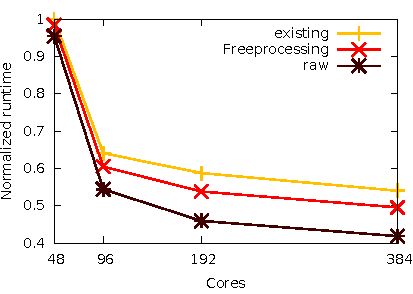
\includegraphics{images/fp/scaling.pdf}

  \caption{Scalability of the PsiPhi simulation. `existing' and
  `Freeprocessing' produce the same outputs via different mechanisms,
  while `raw' produces only restart files.  Freeprocessing's
  overhead is negligible; new output methodologies can even increase
  performance.}

  \label{fig:scaling}
\end{figure}

The simulation authors were enthusiastic about the
\freeprocessor{}.  All the outputs the simulation previously created
were redundant with the restart files.  Furthermore, PsiPhi users
hardcoded postprocessing parameters such as slice numbers into the
simulation source, necessitating a recompile to modify the parameters.
In light of the visualization
options presented by the \freeprocessor{}, the PsiPhi authors elected
to remove
all custom-developed \insitu{} outputs and create only the restart
files.

We therefore reimplemented their outputs in a \freeprocessor{} and
measured the performance of the system under both the old and new
configurations.  As
shown in Figure~\ref{fig:scaling}, not only was the overhead miniscule,
but the
simulation actually ran \emph{faster} with the \freeprocessor{}.  The
performance difference arose from the difference in how PsiPhi and
the \freeprocessor{} organize their writes.  In the
\freeprocessor{}, we calculate the appropriate file offsets on each
rank and output to a shared file directly; the original PsiPhi approach
was to gather the data on the root processor and then do all writing
from there.

% PsiPhi future:
%   specification of slices: *always* want mid-slice
%   want the same slices for every field; no need to change it per-field
%
%
% they typically take 2D slices, and then pull a line out from those
% slices. then they want to see an average (over time) and/or root
% mean square of the data along that line. compare it with a limited
% quantity of measured data. put it all together in gnuplot.
%
% they do this for a series of lines. often they take multiple slices
% and multiple lines.
%
% there is a desire to compare different simulations. done visually, or
% by putting the lines from different runs together in gnuplot.
%
% common workflow:
%
%   1. ssh to remote machine
%   2. run script to get the lines desired into PROFILE/ dir.
%   3. scp PROFILE/ dir to local machine
%   4. run another script to pull out line data into form for gnuplot
%
% this is painful.  would be nice if something could automate all that crap.
%
% desire single UI that knows all the machines you're using and can ssh to
% them and grok this information to display it.  in the end, want to see a
% slice and be able to drag and move it.

\subsection{Enzo}
\label{sec:enzo-example}

\begin{figure}
  \centering
  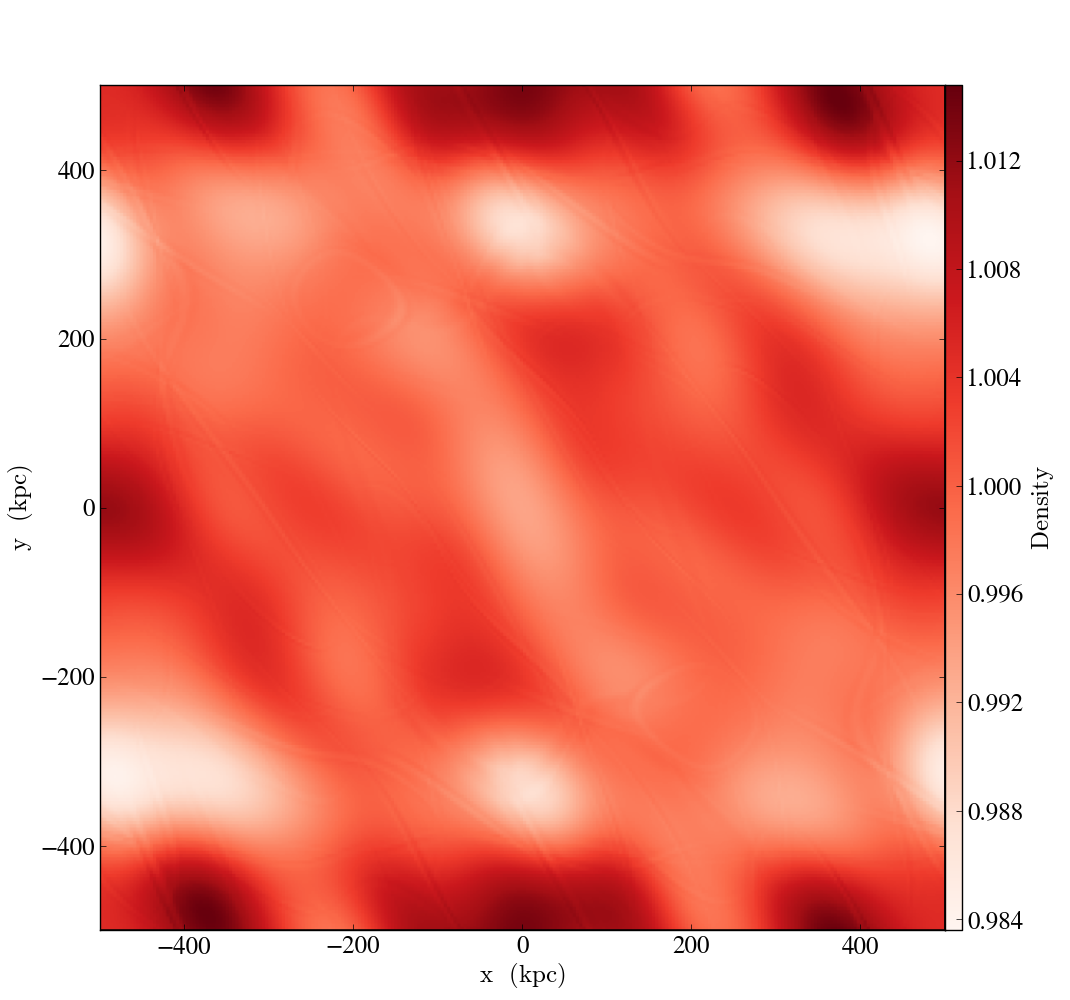
\includegraphics[width=\linewidth]{images/fp/enzo-density}
  \caption{`Density' field generated in situ by the Python
  visualization tool `yt' applied to an Enzo hydrodynamics simulation.
  A \freeprocessor{} exposed the data into Python and a standard yt
  script created the visualization.}
  \label{fig:enzo}
\end{figure}

Enzo is a simulation code designed for rich, multi-physics hydrodynamic
astrophysical calculations~\cite{Enzo:2013}.  It is of special interest
in the visualization community due to its use of adaptively-refined
(i.e., AMR) grids.  Enzo runs in parallel via MPI and CUDA on some of
the world's Top 500 supercomputers, with OpenMP hybrid parallelism
under investigation.  For I/O, Enzo relies on the HDF5 library.

As Enzo is HDF5-based and HDF5 provides all the data semantics
required, the selection of which fields are of interest is the only
required work.  For HDF5 outputs, the symbiont configuration file
specifies the `Datasets' (in the HDF5 sense) of interest as opposed to
a filename; the symbiont assumes that all HDF5 files opened for write
access are a simulation output.

When Enzo was first investigated, HDF5 support was not available in our
symbiont.  Generic HDF5 support in the symbiont required only a day of
effort.  Configuring it to work with Enzo takes seconds. Users must
edit a text file to indicate which field[s] they wish to see.  To work
with
Enzo's \texttt{yt} tool, we utilize the aforementioned
\freeprocessor{} that exposes data into Python and runs a script
(\S~\ref{sec:python}); the script we utilized is a standard yt script,
except that it
pulls its data from the special `\texttt{freeprocessing}' import,
instead of a file.  Figure~\ref{fig:enzo} demonstrates this.  The
100-line \freeprocessor{} is applicable for any \insitu{} application;
the 20-line Python script is specific to yt.

% ngoldbaum: ``I would totally use that for quick viz of a small
% simulation''
%
% Sam Skillman: ``Where do I sign up?''

\subsection{N-Body simulation coursework}

We taught a course in High-Performance Computing during the preparation
of this manuscript.  Among the work given in the course was an
MPI+OpenMP hybrid-parallel N-Body simulation.  We provided our symbiont
to the students along with a simple ParaView script, which would
produce a visualization given one of their timestep outputs.  A sample
visualization is
shown in Figure~\ref{fig:nbody}.

\begin{figure}
  \centering
  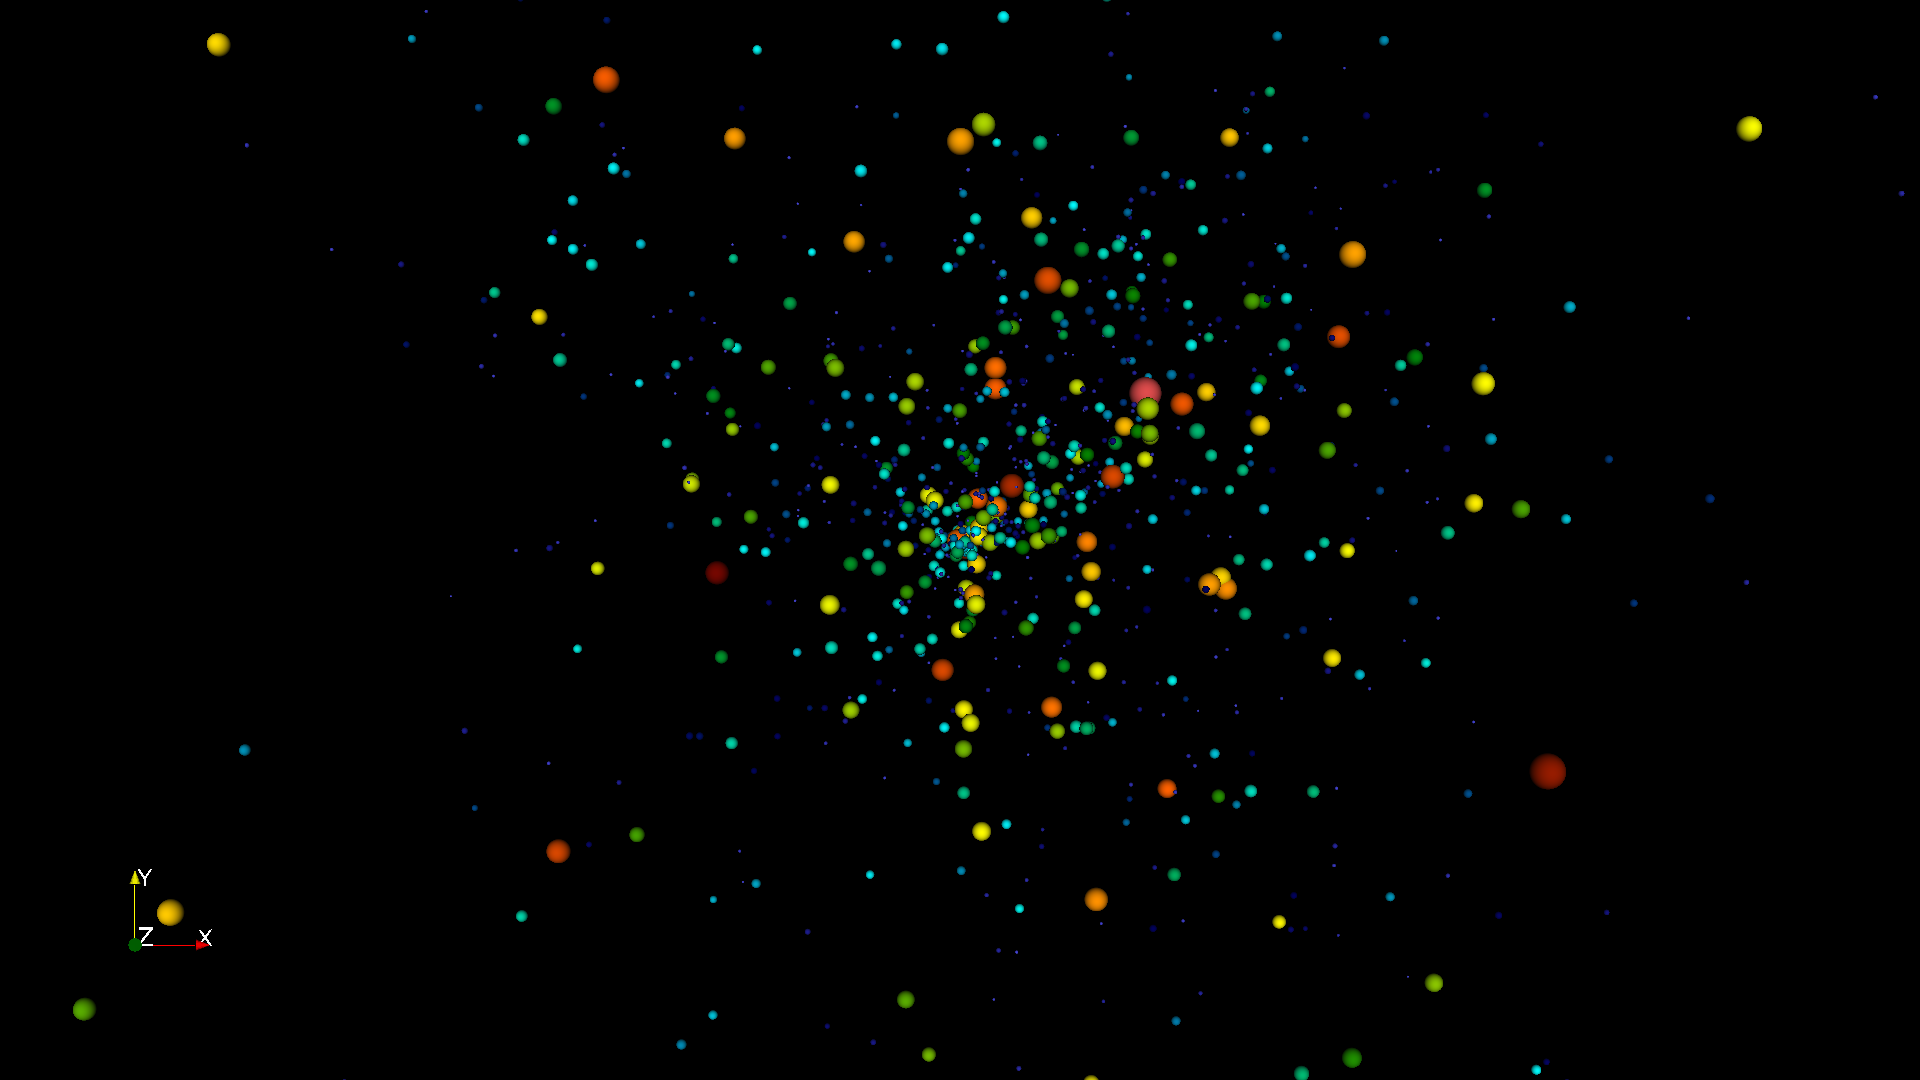
\includegraphics[width=\linewidth]{images/fp/pv-nbody-better}
  \caption{Sample frame from an animation produced from a student's
  simulation using our tool.  The ease of use allowed the student
  to quickly get the tool running, allowing fast and simple visual
  debugging.}
  \label{fig:nbody}
\end{figure}

The flexibility of the system was a boon in this environment.
Visualizing the data in-memory would be difficult. The data were
distributed, and the writes were in ASCII; parsing the data from the
given stream was daunting for undergraduates.  Therefore they elected
to delay launching ParaView until after a timestep completed.  The
system must write and then read particle information from disk, but
visualization was still concurrent with simulation and faster than
serializing the two tasks.  Most importantly, the simplicity allowed
application of the technique in
\textit{tens of minutes}.

% \subsection{Stop the world vs. Asynchronous}
%
% \subsection{In-process vs. Out-of-process}
%
% shared memory vs. just relying on the disk cache
%
% \subsubsection{Out-of-process: launching jobs from within a job}
%
% \subsubsection{Out-of-process advantage over inotify}
%
% it works even over NFS (or other parallel filesystems)

\section{Alternative use cases}
\label{sec:novel}

The ability to hook into \emph{any} data movement operation of a
process enables \freeprocessing{} to create novel applications of
\insitu{} ideas.  In this section, we highlight a couple uses which
makes
\freeprocessing{} unique among \insitu{} tools.

\subsection{Transfer-based visualization}

A heretofore lost opportunity has been in applying visualization
methods to data \emph{during transport from site to site}.  This use
case shares
the primary motivation behind prior \insitu{} visualization work: that
we should do
operations on data while they are \emph{already} in memory, instead of
writing the data to disk and then reading them back. While most if not
all HPC experts agree that---at the largest scale---moving data will
no longer be viable for large data, a large userbase still exists for
which simulation on a powerful remote supercomputer and analysis on
local resources is the norm.

To downplay this drawback, we propose preprocessing during this transit
time.  As an
example of \freeprocessing{} for this novel case, we use it to
instrument the transfer of a dataset using the popular secure copy
(\texttt{scp}) tool.  The system works by intercepting data as it goes
out to or comes in from a socket.  The source of the secure shell
program itself needs no modification; the system could work with any
network service, such as an FTP client or a web browser.

\begin{figure}
  \centering
  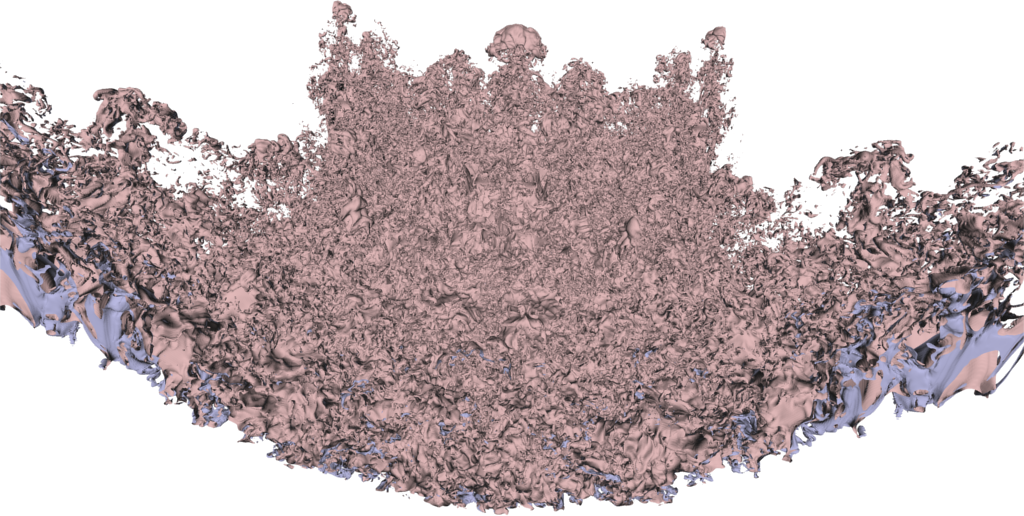
\includegraphics[width=\linewidth]{images/fp/rmeshkov-iso}

  \caption{Richtmyer-Meshkov instability isosurface computed by a
  \freeprocessor{}.  Whereas the \freeprocessor{} could be applied to
  any process that moves data, this particular isosurface was computed
  during network transfer via \texttt{scp}.}

  \label{fig:rm-iso}
\end{figure}

One use case is the computation of an isosurface;
Figure~\ref{fig:rm-iso} shows an example.  A \freeprocessor{} computed
this isosurface of a Richtmyer-Meshkov instability during network
transfer.  This example demonstrates one of the issues with our system:
we needed to modify a marching cubes implementation to work in a
slice-by-slice manner, as opposed to assuming all data were in-core.
Additionally, our marching cubes implementation required at least two
slices to operate, which necessitated a cache in the
\freeprocessor{} to make up for the small writes utilized by
\texttt{scp}.  This buffering and our unoptimized marching cubes
implementation slows down a gigabit-link transfer by 4x.  Although
this still proved faster than transferring the dataset and computing
the isosurface in series, it highlights the pain associated with the
need to rewrite code in a stream processing fashion.  On the other
hand, with the rise of data parallel architectures and the decreasing
memory per core ratio, one might argue that a transition to a stream
processing model is inevitable.

% One
% example is from GPU volume rendering, which requires data organized
% into regular `bricks' for effective paging.  However, as noted by
% recent
% work~\cite{Fogal:2013:Analysis}, this can become a prohibitively
% expensive operation for suitably large data.  The main cost in data
% reorganization is simply loading and writing the file back to disk;
% moving data around in memory is comparatively fast.
%
% The system works by ... calculating the appropriate new
%offset, and transparently re-routing the data to the bricked position.

\subsection{MATLAB}

% MATLAB is a numerical computing environment.  Though it is not
% typically associated with high-performance computing, it nonetheless
% sees extensive use in engineering domains.  It is therefore impossible
% to change the behavior of the program through conventional means, as
% the commercial software is only distributed in binary form.

Users often request methods to read outputs of binary-only commercial
software in tools like
VisIt.\footnote{c.f. ``Using MATLAB to write Silo files to bring
data into VisIt'', \texttt{visit-users} mailing list, February 2014.}.
We implemented a \freeprocessor{} that accepts raw data, reads a
metadata description from a configuration file for semantics, and
exports these data into a Silo file that VisIt can easily import.
Applying this
\freeprocessor{} incurs an additional overhead of 3--10\% on a simple
Julia set calculation in MATLAB, due to the additional data that it
writes.

The alternative of an `export to Silo' MATLAB extension has notable
drawbacks. First, one must compile using the `\texttt{mex}' compiler
frontend, and every major MATLAB update will require a recompilation or
even rewrite.  Second, divorcing the code from MATLAB and its interface
may require significant effort.
In contrast, our \freeprocessor{} is indendendent of the MATLAB version
it instruments, with neither source changes nor a recompilation
required.
Furthermore, the same \freeprocessor{} is applicable in other manners,
such as creating Silo files during a network transfer.

% \TODO{\subsection{Provenance}}

\section{Conclusions}
\label{sec:conclusion}

In this paper we have introduced \textit{Freeprocessing}: an \insitu{}
visualization and analysis tool based on binary instrumentation.  The
method imbues
an existing simulation with \insitu{} powers, with little or---in
some cases---no effort on the part of the simulation author.  The
method's generality enables novel applications, such as visualization
during network transfer or instrumenting software for which source is
unavailable.

The system is, however, not without its drawbacks.  The symbiont
is stable, but customizing the system via new
\freeprocessor{}s can require per-simulation effort.  Furthermore,
the unidirectional communication model precludes simulation steering
applications.
The ability of \freeprocessing{} to insert small,
\textit{ad hoc} bits of code in myriad new places uncovers perhaps
its greatest limitation: increased programmability requires increased
programming.

The work presented here lowers the barrier of entry for a
simulation to indulge in \insitu{} processing.  Previous work on
\insitu{} has largely focused on achieving highly scalable results,
with less regard to the amount of integration effort required.  The
most significant contribution of this work may be that fruitful
capabilities can arise from a modicum of effort.

%Future work in \freeprocessing{} will center around methods for pulling
%additional metadata from the environment, as well as the
%definition of novel \freeprocessor{}s.


\chapter{Metadata inference for \textit{in situ} visualization}
\label{chp:inference}
\newcommand{\addr}[1]{\texttt{#1}}

\section{abstract}

%Visual debugging can be a valuable method to identify and correct
%errors in simulation software.  Current approaches, however,
%are limited by the traditional workflows ascribed to the \emph{use} of
%simulation software. We endeavor to enable \textit{in situ}
%understanding of simulation data.

%The massive size of current and future data is a cause of great concern
%among the visualization community. \textit{In situ} visualization
%provides one of the most promising approaches for dealing with
%the data deluge.  However, the coupling between visualization and
%simulation tool---including the ongoing maintenance such a coupling
%implies---limits the
%application of \textit{in situ} visualization to a small set of
%technically-inclined users.
%
%This coupling is fundamentally rooted in the exchange of metadata that
%describes the data model and data structures of the simulation code to
%the visualization tool.  In this work, we demonstrate that a data model
%and a simulation program are enough information to fully parameterize
%the data structure metadata for \textit{in situ} visualization,
%obviating the need for coupling code and auxiliary descriptions of data
%arrays and information.

Simulation software is routinely used by many disciplines to understand
phenomena when traditional measurement is impractical or even
impossible.  As models increase in detail, however, and the software
stacks underlying high-performance simulation code expand, developing
simulations consequently grows in difficulty.  Verification and
validation of a simulation is therefore an increasingly critical task.
Visualization serves a prominent role in this process, but similar
complexity concerns weigh heavily on the development of new simulation
techniques.

To address the high cost of coupling visualization with simulation
code, we have developed a novel approach that obviates the need for
an explicit connection.  Through instrumented execution of native
x86-64 assembly, we cheaply segment out data of interest and infer the
metadata required for visualization.  As our analysis is binary-level,
it works with any of the languages popular in the high-performance
computing domain.  This transient coupling can be applied or removed
in an \textit{ad hoc} manner.  We demonstrate the utility of the
approach with a number of microbenchmarks and real-world simulations
in use by current researchers.

\definecolor{darkcyan}{rgb}{0.1,0.5,0.6}
\definecolor{darkgreen}{rgb}{0.1,0.6,0.1}
\lstset{
  commentstyle=\color{darkgreen},
  keywordstyle=\color{red},
  identifierstyle=\color{black},
  keywords="size_t",
  frame=none,
  captionpos=b,
  numbers=none,
  numberstyle=\tiny\color{gray},
}

\section{Introduction}

%what/why sim
%vis is necessary
%existing coupling solutions (e.g. VisIt's libsim) are difficult to integrate
%dream: visualization is *concurrent* with simulation development

%data in a simulation program can be considered one of a few (finite)
%  parameterized types
%if we have the parameterized type for a data set, we can create a visualization
%  for it
%most \textit{in situ} tools rely on APIs to transmit this information from
%  simulation to visualization
%the APIs for transmittance are what makes this difficult

%two things make in situ vis hard:
%  * linking in massive software stack for visualization tool
%  * coding to the aforementioned API for communicating data \&\& metadata
%if we could remove these aspects, we're one step closer to the dream.  but how
%do we communicate the metadata without explicit communication?

%simulation does not `do' much, in comparison to most application software
%that is, a simulation spends most of its time in inner loops, repeating the
%  same computation
%this means there isn't too much data that isn't "data of interest": something
%  we might want to visualize
%we can get a small set by automatic means (no strings, etc.)
%when small enough, user interaction can reduce the set to a manageable size
%  \* enzo made 2,028 allocations in a sample run i did.  this is a small \#!

%\todo{histogram of memory lifetimes? can use it to make the point that
%most memory is short-lived}

%\todo{this appears to address Vis people and Sim people, but we're
%publishing it in a PL conference.  Addressing the wrong people, need to
%change focus!}

%\todo{can probably make the point that vis and sim can go together in
%smaller amount of text}

Simulation has seen tremendous growth as a tool to understand problems
from biomedicine to engine design, epidemiology, atmospheric systems,
and many more scientific disciplines. In developing and debugging
such simulations, validation is a difficult yet necessary process.
The inability or cost of performing experimental comparison is often
prohibitive.  Even when measured experimental scenarios exist,
oftentimes comparisons to the measurements are best done in a visual
way.

%% add here that we need to do in situ so that it makes the process feasible

The traditional cycle for simulation-based understanding begins with
editing the simulation's code, running some example systems and dumping
potentially large amounts of data to disk, and finally loading the data
into a visualization tool for analysis.  To accelerate the cycle time
in this `waterfall' process, many simulation authors are turning to
\textit{in situ} visualization: pre-baking the visualization task so
that it can be
produced \emph{while} the simulation is running.  Dynamic control (i.e.
editing of the visualization task at runtime) is possible, but has
remained elusive in practice.

The nature of these as discrete steps is unfortunate.  A simulation
author might not consider visualization until the simulation
itself is fully written.  Yet the ability to \emph{see} the effect of
code modifications on the simulated data could have a profound effect
on the productivity of the simulation author.  We believe part of what
holds back dynamic visualization of simulation data is the difficulty
in integrating visualization tools into simulation development.

% need to find a way to say this that's not offensive to comp.al scientists
These difficulties are twofold.  The first issue is that visualization
software is often orders of magnitude more complex than simulation
software, and the former requires an extensive set of middleware for
its underlying software stack.  The second is common to using any
library: the simulation author must learn the API and data model that
the visualization tool uses to communicate data and metadata.

\cite{Hall:2009:Next50}~note the importance of ``program-analysis strategies to
improve software construction, maintenance, and evolution.''  In this
work, we introduce a methodology for ``0 day'' coupling of simulation
and visualization code.  We remove the need to link in any external
code to the simulation.  The simulation software does not even need to
be recompiled.  The bulk of our contribution is in the form of program
understanding: we demonstrate how to infer which data
are interesting \emph{as well as}---more importantly---the
parameterization of those data that enables visualization.  This
obviates the need for the simulation author to conform to, or even
learn, an external API.

%Some simulation authors are turning to \textit{in situ} techniques for
%effective high-performance visualization, especially as simulations
%begin dumping more data than can be processed via a traditional
%`staged' pipeline.  These techniques consider the complete process of
%understanding phenomena, with simulation and visualization as a single
%intertwined symbiotic stage.  This fuels large efficiency increases, at
%the cost of a measure of flexibility.

%The small scale of the visualization community in relation to the
%simulation community's size has imposed a particular and often
%ill-acknowledged collaborative structure.  Notably, the visualization
%community must produce tools that the simulation community consumes.
%In the case of \textit{in situ} visualization, the visualization
%community produces \textit{in situ} tools, and individual simulation
%authors are tasked with coupling those visualization tools with their
%simulation.
%
%We feel that this merger between simulation and visualization tool
%imposes a significant tax on the simulation author.  Furthermore,
%background dynamics of both communities disenfranchise the simulation
%author to effect this symbiosis: commonly, simulation authors are
%domain experts, and visualization experts come from a computer science
%background.  Frequently, visualization community members have formal
%and practical training in the construction of software, whereas a
%simulation author who is both a domain expert \emph{as well as} an
%experienced software developer is cherished for their abilities.
%
%As an alternative to the status quo in the communities' interaction,
%visual validation, and the traditional \emph{in situ} visualization
%approaches, we propose a novel system that automatically identifies and
%interprets visualizable fields in a running simulation.  No special
%effort is required on the part of the simulation author.  Visualizable
%data is presented concurrently with simulation results and updated
%automatically as the simulation evolves.  The ease of use encourages
%simulation authors to include visual debugging in their regular
%development cycle, much in the way a read-eval-print-loop (REPL)
%encourages users to experiment and evaluate language constructs.

\section{Program analysis and assumptions}
\label{sec:model}

In this section we develop an abstract model of an executing simulation
program.  Our model utilizes a machine that is a significant
simplification from our target architecture of x86-64, but our analysis
only requires this high-level specification.

%While the model is restrictive, architectural realities, the state
%of modern compiler capabilities, and modern software development
%`best practices' make the simplifications largely irrelevant for our
%purposes.  We then use the model to infer data of interest.

\begin{lstlisting}[float=*,label=lst:relaxation,language=C,caption=A code
fragment representative of simulation software.  A large array is smoothed using
a set of nested loops. \texttt{S} is presumed to be a macro that
samples \texttt{data} while properly accounting for edge cases.]
for(size_t j=0; j < dims[1]; ++j) {
  const size_t row = j*dims[0];
  for(size_t i=0; i < dims[0]; ++i) {
    data[row+i] = (S(x-1,y-1) + S(x-0,y-1) + S(x+1,y-1) +
                   S(x-1,y-0) + S(x-0,y-0) + S(x+1,y-0) +
                   S(x-1,y+1) + S(x-0,y+1) + S(x+1,y+1)) / 9.0
  }
}
\end{lstlisting}

The code fragment in Listing~\ref{lst:relaxation} fits the model of the
software of interest to us in this work.  Assuming such code is found
in an environment that greatly emphasizes high-performance implies much
about the code displayed here.  First, the
\texttt{data} array can only be a multidimensional array (even though
its type is one-dimensional).  That array must be heap-allocated using
a single allocation request: simulations routinely deal with data
sizes far larger than typical stack or static memory sizes.  Data flow
analysis would identify
the access of \texttt{data} within the loops of
Listing~\ref{lst:relaxation} as dependent on the loop variables
\texttt{i} and \texttt{j}, though there is little need for such
formality: both the programmer and the compiler would have strong
incentives to hoist the access, were this not the case.  Finally,
\texttt{data}'s dimensionality in this program must be two, and the
number of elements is $dims[0] \times dims[1]$.

\newcommand{\pointsto}[0]{\rightarrow}
\newcommand{\union}[0]{\cup}

\begin{figure}
\begin{eqnarray}
  BaseType &:=& Booleans \union Integers \union FP
    \union Strings \nonumber\\
  Type &:=& BaseType \union Array \union Pointer \nonumber \\
  Memory &:=& Heap \union Static \union Local
    \union Arguments \union Text \nonumber \\
  IPtr &\in& Text \nonumber\\
  T &:=& Memory \mapsto Type \nonumber \\
  B &:=& Memory \mapsto BaseType \nonumber \\
  F &:=& [ addr \in Text, end \in Text ]  \mid \  addr < end \nonumber\\
  W &:=& Text \mapsto F \nonumber \\
  %\textbf{class} & \  Node_{CFG} & \  address \  edges \nonumber\\
  \textbf{class} && \  Node_{CFG} \  address \  edges \nonumber\\
  % we have a hole here: need to say a CFG is a set of Node_{CFG}s.
  \indent CFG &:=& \{ n \mid n = Node_{CFG} \} \nonumber\\
  % note that this definition disallows self-modifying code.  that's OK.
  Wr &:=& (m \in Text) \mapsto (n \in (Memory \setminus Text)) \mid m \neq n
    \nonumber\\
  Rd &:=& (m \in Text) \mapsto (n \in (Memory \setminus Text)) \mid m \neq n
    \nonumber\\
  % we have a hole here: need to say a CFG is a set of Node_{CFG}s.
  BB &:=& F \mapsto CFG \nonumber \\
  K &:=& Text \mapsto Node_{CFG} \nonumber\\
  H &:=& Node_{CFG} \mapsto Boolean \nonumber\\
  L &:=& Node_{CFG} \mapsto Integer \nonumber
 %Q := Text \mapsto F\\
%  \textbf{class} \  ND \  base \  length \  dims \  ndims\\
%  \indent | base \pointsto m \in Heap\\
%  \indent | B(base) \in FP\\
%  \indent | T(dims) \in Array \union Pointer\\
%  \indent | B(dims) \in Integer\\
%  \indent | T(ndims) \in Integer\\
%  \indent | ndims > 0\\
%  \indent | Wr(IPtr) \in [ base, base + length ]\\
%  \indent | b \in BB(W(IPtr)) \land IPtr \notin b \land H(b)
%    \land L(K(IPtr)) > L(b)\\
\end{eqnarray}
  \caption{Definitions for abstract machine and analysis based on
  properties of control flow.}
  \label{fig:model}
\end{figure}

We use the formalisms given in Figure~\ref{fig:model}.  We consider an
abstract machine described by an
\textit{instruction pointer} and the current state of
\textit{memory}.
%\begin{math}
%  \indent IPtr \in Text\\
%  \indent Memory := Heap \union Static \union Local \union Argument
%    \union Text\\
%\end{math}
The instruction pointer is assumed to advance automatically, and memory
operations consist of reads and writes that map an address to a mutable memory
location.
%\begin{math}
%  \indent Wr = m \in Text \mapsto n \in (Memory \setminus Text) \mid m \neq n\\
%  \indent Rd = m \in Text \mapsto n \in (Memory \setminus Text) \mid m \neq n\\
%\end{math}
Note that this definition denies self-modifying code.  Memory is assumed to be
\emph{typed}, with a small set of available types.  The $T$ and $B$ mappings
define mappings from memory locations to type information.
%\begin{math}
%  \indent BaseType = Booleans \union FP \union Integers \union Strings\\
%  \indent Type = BaseType \union Array \union Pointer\\
%\end{math}
%and mappings from memory locations to type information.
%\begin{math}
%  \indent T = Memory \mapsto Type\\
%  \indent B = Memory \mapsto BaseType\\
%\end{math}

The running process is assumed to consist of a series of
\textit{functions}, $F$, that are defined as the functions' upper and
lower addresses.  We will make use of an inverse mapping $W$ that
allows us to identify a function from the
current instruction pointer.
%\begin{math}
%  \indent F = [ addr \in Text, end \in Text ] \mid addr < end\\
%  \indent W = Text \mapsto F\\
%\end{math}
We build local \textit{control flow graph}s (CFGs) that describe the potential
execution paths.  These graphs are represented as a set of \textit{nodes} that
contain an entry \textit{address} as well as a set of \textit{edges}.
%\begin{math}
%  \indent \textbf{class} \  Node_{CFG} \  address \  edges\\
%  % we have a hole here: need to say a CFG is a set of Node_{CFG}s.
%  \indent CFG = \{ n \mid n = Node_{CFG} \}\\
%\end{math}
We build these CFGs based on the
function address range.  We define a mapping $K$ that allows
us to identify nodes in the control flow graph from an instruction
address.
%\begin{math}
%  \indent BB = F \mapsto CFG\\
%  \indent K = Text \mapsto Node_{CFG}\\
%\end{math}
We define two final mappings from a node in the control flow graph: 1)
a predicate identifying \textit{loop headers}, and 2) a mapping for the
calculated \textit{loop depth}.  The headers $H$ correspond to the
basic blocks that contain the loop test.  In Listing~\ref{lst:relaxation},
the basic blocks containing \texttt{j < dims[1]} and \texttt{i <
dims[0]} would be the loop headers.  Loop depth is the nesting level of
the provided basic block.  In Listing~\ref{lst:relaxation}, the
assignment to \texttt{row} has a depth of $1$.  The assignment to the
element in \texttt{data} has a loop depth of $2$.
%\begin{math}
%  \indent H = Node_{CFG} \mapsto Boolean\\
%  \indent L = Node_{CFG} \mapsto Integer\\
%\end{math}

%\noindent \begin{math}
%  BaseType := Booleans \union Integers \union FP \union Strings\\
%  Type := BaseType \union Array \union Pointer\\
%  Memory := Heap \union Static \union Local \union Arguments \union Text\\
%  IPtr \in Text\\
%  T = Memory \mapsto Type\\
%  B = Memory \mapsto BaseType\\
%  F := [ addr \in Memory, end \in Memory ] | addr < end\\
%  W := Text \mapsto F\\
%  % note that this definition disallows self-modifying code.  that's OK.
%  Wr := (m \in Memory) \mapsto (n \in Memory) | m \neq n\\
%  \textbf{class} \  Node_{CFG} \  address \  edges\\
%  % we have a hole here: need to say a CFG is a set of Node_{CFG}s.
%  BB := F \mapsto CFG\\
%  K := Text \mapsto Node_{CFG}\\
%  H := Node_{CFG} \mapsto Boolean\\
%  L := Node_{CFG} \mapsto Integer\\
%  %Q := Text \mapsto F\\
%  \textbf{class} \  ND \  base \  length \  dims \  ndims\\
%  \indent | base \pointsto m \in Heap\\
%  \indent | B(base) \in FP\\
%  \indent | T(dims) \in Array \union Pointer\\
%  \indent | B(dims) \in Integer\\
%  \indent | T(ndims) \in Integer\\
%  \indent | ndims > 0\\
%  \indent | Wr(IPtr) \in [ base, base + length ]\\
%  \indent | b \in BB(W(IPtr)) \land IPtr \notin b \land H(b)
%    \land L(K(IPtr)) > L(b)\\
%\end{math}

Using this model of program execution, we consider the problem of
automatically identifying memory regions that house data that a user
would want to visualize.  We model these as a set of constraints on
type classes.  An instance of the type class allows one to visualize
data within a simulation.

%, with constraints sourced from the observation of program
%execution.  In this way, we can visualize the data \emph{as} it is
%modified by the simulation.

%\todo{haven't actually convinced myself this is a type class in the
%correct sense of the term, based on my limited understanding of it.
%maybe `constrained parametric type' is better. it certainly resonates
%better with me...}

The type we search for is the $N$-dimensional (``ND'') data array.
This type is parameterized by a \texttt{base} address, a
\texttt{length} (in bytes), the number of
dimensions \texttt{ndims}, an array of dimensions \texttt{dims}, and
finally the type of the data.
% need a 'comment' column to summarize important considerations!
\begin{eqnarray}
  \indent \textbf{class} \ & ND & \  base \  length \  ndims \  dims \  type
    \nonumber\\
  \indent &\land& base \pointsto m \in Heap\\
  \indent &\land& B(base) = type\\
  \indent &\land& T(dims) \in Array \union Pointer\\
  \indent &\land& B(dims) \in Integer\\
  \indent &\land& T(ndims) \in Integer\\
  \indent &\land& ndims > 0\\
  \indent &\land& Wr(IPtr) \in [ base, base + length ]\\
  \indent &\land& \exists b \in BB(W(IPtr)) : \nonumber\\
    && \land \ IPtr \notin b \nonumber \\
    && \land \ H(b) \nonumber\\
    && \land \ L(K(IPtr)) > L(b)
\end{eqnarray}
We use the $\pointsto$ notation to mean ``points to''; the first
constraint simply states that the data of interest live on the heap.
As simulation data is large, it cannot fit on the stack or even in
statically initialized memory.  The second constraint conveys that the base
type matches a parameter of our model, such as $FP$ (floating point).
The third and fourth constraints dictate that the dimensions are stored
in a linear list of integers, and the fifth and sixth say the variable
that describes the length of that list is a simple integer.

The 7th and 8th constraints are complex and intertwined.  First, the
application must write into the the relevant memory block.  Secondly,
the basic block where the data are written is deeper than another basic
block that contains a loop header.  That is to say that the data access
is within a loop.

The formulation gives rise to a pattern matching problem.  The
\texttt{\textbf{class}}es of interest are the patterns, and the space
to match within is the running process' \texttt{Memory} and
\texttt{IPtr}.  In Listing~\ref{lst:relaxation}, the parameter bindings are:
\texttt{data} for \texttt{base}, the size of the allocation (not shown, but
assumed to be \texttt{dims[0]*dims[1]*sizeof(float)}) for
\texttt{length}, \texttt{dims} for \texttt{dims}, and $2$ for
\texttt{ndims}.

\section{Implementation}

Our task is to match the given constraints with an executing process.
Working with the executing process is imperative given our goal of
concurrently visualizing the data as it is computed.  Furthermore, some
constraints---notably those involving the value of variables, such as
the instruction pointer or a variable to be matched such as $ND$'s
(``$N$-Dimensional'')
\texttt{ndims}---can only be determined at runtime.  Therefore the
system must include some level of dynamic analysis.  For simplicity and
applicability, we do all of our analysis during runtime and directly on
the binary under execution.

We target unstripped binaries with debug information.  This gives us
robust type information as well as simplifying implementation.
\cite{Reps:2010:Bottom} give detailed information on how this
simplifies the task. Our use case of simulation developers creating and
debugging their simulation coincides with this input: the environment
would make it likely that users would compile with debug information
even without our tool in use.

A notable advantage of targeting binaries is that it is
language-agnostic.  C, C++, and Fortran are the dominant programming
languages used in high-performance computing environments.  By parsing
machine code for our target x86-64 platform we simplify the entire
system by dealing ostensibly with a single input language.  %A %set of
%reasonable assumptions for the executing process and environment %is
%given in
%\S{\ref{sec:assumptions}}.
Given these assumptions and the simplifications of our model in
Section~\ref{sec:model}, the transformation from a language such
as C to assembly language preserves all information of relevance.

Our system uses a \texttt{ptrace(2)}-based supervisor for the target
program.  We induce small changes to process execution that are
invisible under memory-safe operation, and our efforts are rewarded
through efficient notification of events in the simulation.  An example
event is the access of a data array previously identified as housing
visualizable data.
When such events are \emph{not} occurring, simulation execution
proceeds at native speed.

% governed by a finite state machine (see fig 1)
% every memory (allocation) region is at some state in state machine
% we don't actually need to instantiate a state machine for each allocation
%% those in the 'null' state can be ignored

Heap-allocated memory is the centerpiece of each
\texttt{\textbf{class}} we search for.  Any heap-allocated memory
region is potentially of interest for us, though we note that at any
given moment, most allocations provide uninteresting input from a
visualization standpoint. We model each memory region by the finite
state machine given in
Figure~\ref{fig:fsm}, with the initial `null' state represented
implicitly for efficiency reasons.  All memory is assumed to be in the
`null' state initially.  Memory regions change their state based on
events observed in the simulation process.  Note that a single event
may cause a transition in multiple regions.

\begin{figure}
  \centering
  \begin{tikzpicture}[scale=1.0,thick,align=center]
    \node[state](null){null};
    \node[state,right of=null](mloc){malloc};
    \node[state,above of=mloc](mret){mreturn};
    \node[state,right of=mret](allow){allow};
    \node[state,below of=allow](kill){kill};
    \node[state,below of=kill](deny){deny};
    \node[state,left of=deny](hdr){header};
    \path[line](null)--(mloc);
    \path[line](mloc)--(mret);
    \path[line](mret)--(kill);
    \path[line](mret)--(allow);
    \path[line](allow)--(kill);
    \path[line](allow)--(hdr);
    \path[line](allow) to[out=-20,in=0] (deny);
    \path[line](hdr)--(kill);
    \path[line](hdr)--(deny);
    \path[line](hdr) to[out=180,in=120,distance=1cm] (hdr);
    \path[line](deny) to[out=20,in=0] (allow);
    \path[line](deny)--(kill);
    \path[line](kill) to[out=-200, in=60] (null);
  \end{tikzpicture}

  \caption{Finite state machine governing memory regions of interest.
  Regions transition between the states based on events observed in
  the observed simulation process.  Basic information is obtained in
  the \emph{malloc} and \emph{mreturn} states.  The \emph{allow} state
  initializes parameters for visualization and enables unfettered
  access to the memory. \emph{header} states build up the dimensions of
  the data.  The \emph{deny} state is used to detect future accesses.
  Memory is \emph{kill}ed when it is deallocated.}
  \label{fig:fsm}

\end{figure}

\subsection{Memory tracking}

The events that instantiate the memory regions of interest are
allocation requests.  We implement the event notification by
inserting a breakpoint on \texttt{malloc} calls, and can thereby track
all heap memory in use by an application.  When the breakpoint is hit,
we examine the argument to determine the size of the allocation.  A
second breakpoint is inserted when
\texttt{malloc} returns, to read the pointer the call produced.
Together, these allow us to identify the base addresses and lengths
of all the heap memory in the process.  Overhead for this aspect is
predominantly context switching from the simulation process to the
supervisor.

The $ND$ \texttt{\textbf{class}} has constraints that include the
function pointer at the time the data (memory within \texttt{base} and
\texttt{base} $+$ \texttt{length}) were accessed.  Unfortunately, the
\texttt{malloc}-based tracking only informs us what dynamic memory
\emph{exists} in a process, not when it is \emph{accessed}.
Traditional debugger watchpoints are implemented (on x86*
architectures) using a finite set of debug registers; these would be
quickly exhausted in our case.  Finding instructions that modify memory
and inserting checks is a viable
alternative, but \cite{Antoniu:2001:PFault} previously showed this to
be inefficient.

%Tracking the pointer via symbolic interpretation may be possible, but
%quickly runs up against difficult-to-solve aliasing problems, and is
%unlikely to be computationally viable.

We use a technique from distributed shared memory environments that
induces a segmentation fault when the data of interest are accessed.
We subtly alter every allocation of interest so that it not only
allocates the memory, but also protects the memory region, as per the code
shown in Listing~\ref{lst:malloc}.  When the process attempts to alter
the data of interest, the memory
protection hardware traps and our supervisor is notified\footnote{The
program may also trap because it has a bug that causes an invalid
memory access.  Such programs are beyond the scope of this work: who
would want to visualize the calculations of a broken program?  Still,
we note that we can discern the invalid memory access case and notify
users of the error's location.}

%\begin{minipage}{\linewidth}
\begin{lstlisting}[label=lst:malloc,language=C,caption=Replacement \texttt{malloc}
implementation used for tracking field access.]
void* alignedalloc(size_t n) {
  void* mem;
  if(posix_memalign(&mem, getpagesize(), n) != 0) {
    return NULL;
  }
  if(mprotect(mem, n, PROT_READ) != 0) {
    free(mem);
    return NULL;
  }
  return mem;
}
\end{lstlisting}
%\end{minipage}

As this segmentation handling is expensive, we only perform access
detection for the first access within a function.  After it detects a
segmentation fault in the simulation process, our supervisor changes
the memory protections to allow unfettered access to the data.  At
the same time, we insert a breakpoint at the caller of the current
function, so that we may re-enable memory protection and detect
subsequent accesses of the same data.

The astute reader may note that memory protection is possible only on
page-aligned data.  We therefore require a modified \texttt{malloc}
implementation that calls \texttt{posix\_memalign} (to allocate the
page-aligned memory) followed by \texttt{mprotect} (to set up the
desired memory protections).  Since we do not require the user to link
against any runtime, adding a function in the traditional way is not
viable.  Instead, we inject our modified \texttt{malloc} implementation
directly into the executing process image after static initialization
has completed.  We modify the instruction pointer when a
\texttt{malloc} occurs to instead jump to our page protection
allocation routine.

\subsection{Control flow}

The memory tracking described above enables our supervisor to track
most of the events it needs.  To pinpoint the remaining events we use
analysis based on the local control flow.  When a region is accessed,
we build the local control flow graph for the currently-executing
function.  Our supervisor computes common compiler analysis
information such as dominance~\cite{Torczon:2007:Compiler} and uses
the results of this analysis to define per-node depth as well as to
identify
loop headers, as in Figure~\ref{fig:cfg}.

There are some known limitations to this approach.  One is its
fragility in the presence of
\texttt{goto} statements.  If the \texttt{goto} crosses a loop
boundary, then the depth information calculated may be incorrect, and
the algorithm will not compute a proper loop tree.  Fortunately, in
practice this is rare; we have not encountered this case in simulation
programs of interest.

%% drop this?  it sounds really negative.
Some compiler optimizations pose issues as well.  Loop transformations,
such as loop tiling or fission, can cause issues with the inference we
perform.  While it may be possible to workaround these on a case by
case basis, we reiterate that our use case is primarily in the domain
of simulation \emph{development}.  As such, these optimizations can
simply be disabled during development to allow use of the tool.

%% relies on assumptions:
%%%% data are within the loop because the loop is relevant
%%%% => loop bounds imply bounds on the data
%%%% the application does not use gotos in these tight loops
%%%% loop tiling etc. are not performed
\begin{figure}
  \centering
  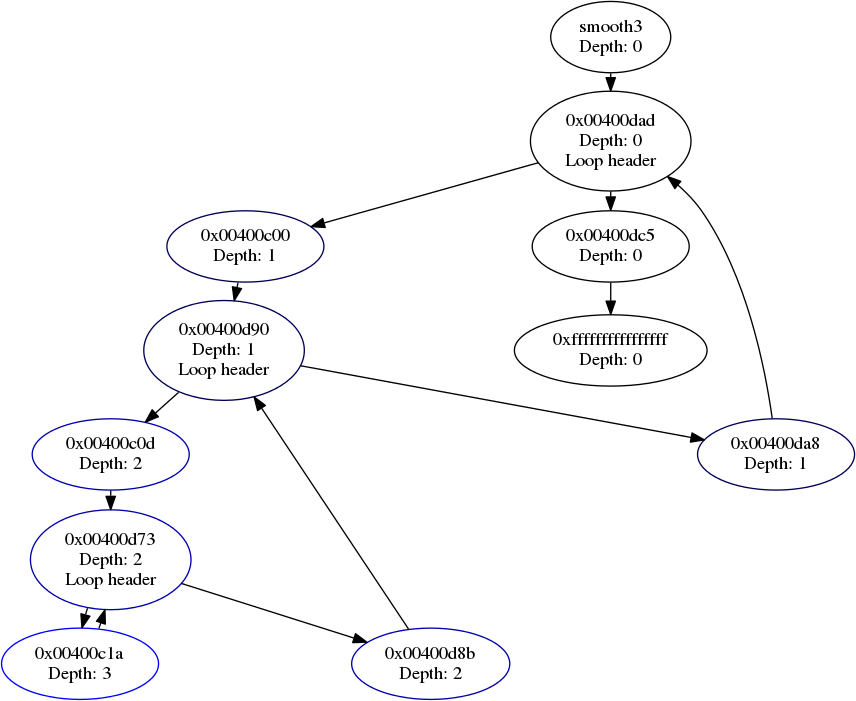
\includegraphics[width=\linewidth]{images/dbg/s3}

  \caption{Simplified control flow graph for a small function that
  smooths a 3D array.  Analysis identifies loop headers and the nesting
  level (`Depth') of each basic block.  On access, the loop tree is
  traversed to determine the dimensionality of the array.}

  \label{fig:cfg}
\end{figure}

\subsection{Symbolic execution}

As described in the $\textbf{class} \ ND$ of Section~\ref{sec:model},
we assume a relation between loop headers and the basic blocks that are
contained within those loops and accessing memory.  The loop variable
must be involved: if it were not, the access would be loop-invariant
and hoisted out of the loop, either explicitly by the programmer or
implicitly by the compiler.  We assume a stronger relation, however:
that the loop conditions imply the dimensionality of the memory regions
accessed therein.

%\todo{this is very strong, which is okay, but we have no proof, which
%is not okay} Barring absurd instruction sequences (e.g. a series of
%\texttt{NOP}s), there are a finite number of ways that a compiler might
%encode a loop header.

Since the loop header decides whether the loop will continue or not, it
must reference both the induction variable and the loop bound.  If we
can identify which operand is which, then we will know the loop bound.

The comparison instruction itself has no ordering or other method to
distinguish the operands.  We utilize the debug information to decide
whether each operand is a local, reference to a global, or a constant.
When exactly one of these references is a local, we consider it the
induction variable; the other variable gives the loop's bound.

\begin{lstlisting}[label=lst:header,caption=Instructions within a
sample loop header.  Both the induction variable and the loop bound
appear as arguments to the \texttt{CMP} instruction.  The preceding
instructions are still necessary for distinguishing between the two
variables.]
  MOV %rdx, [%rip+0x20507]
  MOV %rax, [%rpb-0x60]
  CMP %rdx, %rax
  JB -0x275
\end{lstlisting}

%% bad: 'we'd like to do X, but it's too impossible, so we do Y.'
Ideally, we would simply examine the comparison instruction to identify
the operands and infer the loop bound. Unfortunately a myopic view of
this single instruction is insufficient for operand classification.
The instruction sequence for a loop header generally follows the
pattern that
Listing~\ref{lst:header} follows: first, the bound and induction
variables are loaded into registers; second, the comparison is
performed; and finally, a conditional jump exits the basic block.  The
induction and bound variables are referenced in the basic block, but
the comparison itself often operates on registers that have erased the
original source of the data.  Concretely, in Listing~\ref{lst:header},
\texttt{\%rax} itself is less relevant than the \emph{source} of
\texttt{\%rax}'s
value: the memory pointed to by \texttt{\%rbp-0x60}.  Since the variable
is relative to the frame pointer, this tells us that it must be an
argument or a local variable.  Debug information for the program can
discriminate between these final two cases for us.

% the LH basic block must reference both the induction variable as well as the
%   end criterion
%%%% we could prove this empirically.  just take enzo, for example, compute the
%%%%  CFG for every function, and then analyze each loop header to check if it
%%%%  loads two things.
% "myopic view of CMP" is not enough
%% no ordering to the operands! how do we identify what kind of thing we have?
%%% the induction variable can be safely assumed to be a local
%%% the end criterion *might* be local, but more likely a constant, argument
%%%   to the current function, or a global.
%%%%% again, we could empirically verify: is every CMP in an enzo LH a
%%%%% combination of a local and a (constant | argument | global)?
%% we can solve the type information problem using debug information
%%% but again: myopic view of CMP is not enough

\begin{algorithm}
  \caption{Symbolic interpretation algorithm for identifying data sources.  A
  virtual register set is tracked within loop-free basic blocks to identify
  the source of operands to specific instructions.  These sources are then
  used to lookup debug information and interpret register contents.}
  \label{alg:sinterp}
  \begin{algorithmic}[1]
    \State register[*] := UNKNOWN
    \State instruction := bb$_{addr}$ \Comment first instruction in loop header
    \Repeat \Comment foreach instruction in the basic block
      %\Comment cast to instruction of appropriate type
      \State \Comment cast to instruction of appropriate type
      \If{instruction.Opcode = MOVE}
        \State mov := (MovInstruction)instruction
        \If{mov.source $\in$ register}
          \State register[mov.target] := register[mov.source]
        \ElsIf{mov.source is an address}
          \State register[mov.target] := mov.source + \\
                                         \hspace{6em}memdiff[mov.source]
        \EndIf
      \EndIf
      \State \Comment Track address modifications
      \If{instruction.Opcode = ADD}
        \State add := (AddInstruction)instruction
        \If{add.dest $\in$ register $\land$ \\
            \hspace{3.75em} register[add.dest] $\neq$ UNKNOWN}
          \State register[add.dest] += add.source
        \EndIf
        \If{add.dest $\in$ memory}
          \State memdiff[add.dest] += add.source
        \EndIf
      \EndIf
      \State instruction := next(instruction)
    \Until instruction.Opcode = CMP
  \end{algorithmic}
\end{algorithm}

Algorithm~\ref{alg:sinterp} derives the source of the data in the loop
header's comparison instruction.  We track a virtual register set
and the set of memory changes over the basic block of the header's
instruction sequence.  Instructions that modify a register or memory
are tracked, though only the differences to memory operations are
saved.  The interpretation terminates at the basic block's comparison
instruction, and outputs the symbolic register file.  We can use this
register file to identify the source of the data within a comparison
instruction.

%% again, a negative and really minor case.  can't we just drop this?
It can occur that the loop bound is also a local variable, making
both the induction variable and the bound both local.  This impedes
our ability to discern the bound operand.  However, we note that this
situation is unlikely to occur in practice.  If the dimensionality of
the array does not change during execution of the function, then this
local variable for the bound should also not change: in this case,
the compiler is likely to elide the variable in favor of a constant.
Our fallback case is to choose the larger of the two values in the
comparison, however we note that we have not yet hit this case in
simulation code utilized thus far.

Once we have identified the source of the data in the comparison
instruction, we allow the simulation to run to that point.  We use
\texttt{ptrace(2)} to read the value for the loop bound.  To interpret
the value, the virtual register set gives the key for the debug
information needed.

%Integer-based or pointer-based indices is at present an input to our
%model that the user must specify, with ill-developed semantics for
%the pointer case.  In the future, we hope to detect this case using
%debug information to automatically choose between the two.  Pointer
%comparisons as opposed to integer indices may pose issues due to the
%ambiguous mapping from the addresses to indices accessed.  For the
%future, we plan to assume a linear traversal of the data and compute
%the indices based on the allocation's type as well as the starting and
%ending indices.  In practice, this case happens so rarely in simulation
%code that we simply ignore loops of this type.

Each iteration of this process gives a single loop bound.  By following
the
state machine in Figure~\ref{fig:fsm} and setting breakpoints up the
chain of the loop tree, we derive the full set of bounds.  At the
function boundary, we enter the `deny' state and re-enable memory
protection for that region.

\section{Evaluation}

%\todo{be more excited about how great this is}
%
%\todo{constantly mentioning the drawbacks and "the 1\%" cases that
%fail, but they're not a big deal---mention those later}

% our stuff is the greatest thing since sliced bread

% already found an indexing error in an image smoothing application
%% image: an image side-by-side with a smoothing error that skews in X

% get a figure of a (pretty!) volume rendering in here

\textit{In situ} visualization is commonly applied in large-scale
parallel simulations in order to reduce the cycle time from simulation
setup to data understanding.  The approach is primarily motivated by
performance: visualization that runs concurrently with the simulation
does not need the costly data loading step common at the start of most
visualization pipelines.  Our thesis is orthogonal to this original
purpose: that \textit{in situ} visualization is useful during
\emph{development} to visually verify the calculations performed
therein.

%\begin{figure}
%  \centering
%  % \includegraphics ...
%
%  \caption{Original image (left) and image smoothed by an incorrect
%  smoothing algorithm (right) that skews the image in X.  The indexing
%  error is readily apparent from the preview visualization provided.}
%
%  \label{fig:smootherr}
%\end{figure}

%Figure~\ref{fig:smootherr} details an error uncovered in an image
%processing routine in some software the authors' lab was concurrently
%developing.  There was an indexing error relative to one of the loops'
%induction variables, causing the issue on the right.  Viewing the
%result of the algorithm immediately exposes the error.

We are integrating more advanced visualization techniques into the
software at present.  Figure~\ref{fig:volren} shows a volume rendering
for the volume of tissue activated in a biomedical simulation.  The
image was generated using the
ImageVis3D~\cite{Fogal:2010:Tuvok} desktop volume rendering package.
The connection of our instrumentation suite and this visualization tool
presently relies on serialization to and from files due to limitations
of ImageVis3D, but we hope to rely on in-memory transfers in the near
future.

\begin{figure}
  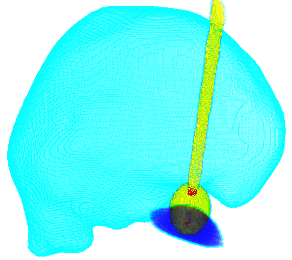
\includegraphics[width=\linewidth]{images/dbg/brain}

  \caption{Volume rendering of the volume of tissue activated from
  a biomedical simulation of deep brain stimulation.  Array shape
  information and data were read from the running simulation and
  serialized to disk, while a concurrent process made the data suitable
  for import into a volume rendering tool.  No user intervention was
  required, beyond setting the transfer function to derive the color
  information.}

%  \caption{Volume rendering of the temperature field from a
%  \textit{PsiPhi} simulation.  Array shape information and data were
%  read from the running simulation and serialized to disk, while a
%  concurrent process made the data suitable for import into a volume
%  rendering tool.  No user intervention was required, beyond setting
%  the transfer function to derive the color information.}

  \label{fig:volren}
\end{figure}

\subsection{Performance}
\label{sec:performance}

A high performance tool encourages simulation authors to integrate that
tool into their daily development routines.  Few developers integrate
useful tools such as Valgrind into their rapid edit-compile-test
cycles, in part due to performance. This functionality is instead
relegated to pre-commit or even nightly testing, limiting the
effectiveness of some memory debugging tools.  Our goal is to enable
visualization that is not only easy to set up, but also cheap enough
that developers leave the tool enabled during daily development.

%\begin{figure}
%  % \includegraphics....
%  %% bar graph of performance w/ and w/o our instrumentation
%
%  \caption{Our `MallocTrace' tool watches for and reports allocation
%  and deallocation requests, producing a report that would be useful in
%  identifying the most promising locations to reduce the application's
%  memory footprint.  It uses breakpoints heavily but no memory access
%  protection; the relatively low overhead indicates that program
%  interruption and interrogation is lightweight.  Software that
%  performs many allocations may experience higher overheads.}
%  \label{fig:mtrace}
%\end{figure}

We therefore consider multiple aspects of performance.  We induce an
overhead in the simulations that we execute by interrupting them at
key points, as well as by minor adjustments to program execution.  The
performance of our supervisor itself is also of interest, as it must
manipulate large symbol tables, construct control flow graphs from
instruction streams, and interpret some instructions to uncover loop
indices.

The approach is evaluated with a set of relevant test programs.
\textit{Linpack} is the matrix-vector multiplication benchmark of
floating point performance that is used to rank supercomputers in the
popular `Top500' list. \textit{Relax} is a program that identifies
the steady state for the case of a plane connected to a constant heat
source.  The program's ratio between function calls and accessing the
data to be visualized is at parity, stressing the memory access and
analysis aspects of our supervisor. \textit{PsiPhi} is a real-world
computational fluid dynamics solver that focuses on Large Eddy
Simulation (LES) of flows that include combustion and other types of
chemical reactions~\cite{Proch:2014:PsiPhi}. \textit{allocs} is a test
program that simply allocs and frees memory without ever acessing it.

Figure~\ref{fig:performance} looks at multiple aspects of performance
across this set of programs.  The red `Uninstrumented' bar details the
execution time without our instrumentation applied, representing an
upper bound for performance.  `Trace' inserts breakpoints at
`\texttt{malloc}', `\texttt{free}', and their return addresses,
measuring what it costs to start and stop the execution of the
simulation program.  Simulations which utilize more regions of dynamic
memory will see higher overheads due to this aspect.  However, the
graph does not capture the phased nature of these processes: generally,
they include a startup phase that allocates memory and initializes
inputs, followed by a computational phase that computes.  As simulation
sizes increase, the initialization phase holds constant whilst the
compute phase scales polynomially.

`Allocations' is a more expensive variant of the `Trace' benchmark.
In addition to allocation interception, this version reads relevant
information from the client process so that it may generate a report
of the [de]allocations made by the process.  The traces this algorithm
creates might be useful in producing and analyzing heap usage over
time, in the same manner as Valgrind's
`Massif'~\cite{Nethercote:2006:Massif}.  We note that this adds little
additional overhead to the instrumentation, demonstrating that reading
memory from the process is cheap.

%As demonstrated by Figure~\ref{fig:mtrace}, the overhead for program
%interruption tied to allocation tracking is low.  All programs profiled
%follow the model of allocating the required memory up front and keeping
%it active for the lifetime of the process.  Thus, most overhead for
%allocation tracking is in a one-time startup phase.  During the
%processes' compute phases, allocations tend to come from external
%libraries, such as the HDF5 file I/O middleware.

`Full' in
Figure~\ref{fig:performance} details overheads for the full gamut of
our analysis techniques.  Conflating the results, however, are filters
that can be applied when more analysis is performed.  As one example of
these
filters, `Full' identifies the caller of \texttt{malloc} and ignores
the allocation if the
memory is an internal \textit{glibc} buffer.  With the extra
information gained from this additional work, `Full' can in many
cases realize that an allocation region is not interesting.  It then
removes the item from the set of memory it tracks, thereby reducing the
overhead induced.  If the overhead of tracking the memory exceeds that
of the analysis, then this variant will actually be cheaper than the
more na\"ive implementations.

% allows comparison of the overheads induced
%by different aspects of the instrumentation.  In particular, it shows
%that the access detection based on page protection has approximately
%the same complexity as the allocation tracking.  For both cases, few

In all cases, a limited number of allocations and accesses results in
near-native performance.  The
\textit{Linpack} benchmark shows this best, as it performs a single
allocation and the array is accessed entirely when it is accessed
at all---the spatial locality is extremely high.  Thus the natural
inclination of the programmer to seek spatially-local accesses
is also the best performance case for our instrumentation.  The
high-performance computing community goes a step further than spatial
locality to advocate high
`arithmetic intensity': the use of a \emph{single} value in \emph{many}
instructions.  Such a focus goes even further towards amortizing our
penalty on first accesses across the larger dataset.

% graph: for `full': stacked bar graph with CFG time,
%  symbolic exec time, symbol table loading, and type lookup time all separate?

\begin{figure}
  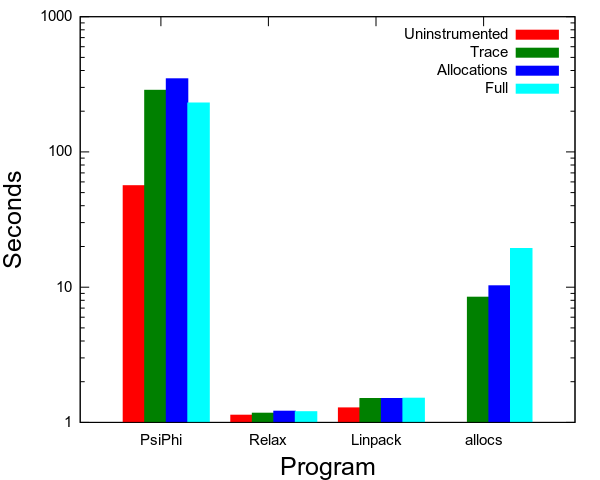
\includegraphics[width=\linewidth]{images/dbg/mtrace/performance}

  \caption{Performance of our evaluation programs under different
  instrumentation scenarios. Note logarithmic scale.  `Uninstrumented'
  is performance of the simulation without our interference. `Trace'
  interrupts for allocations; `mallocs' \emph{reports} allocations as
  well, which requires reading more data from the instrumented program.
  `Full' does allocation tracking, access detection, analysis, and
  visualization of the data.}

  \label{fig:performance}
\end{figure}

In practical terms, the performance scales with 1) the number of
allocations the program performs, and 2) the number of allocations that
are tracked and provide source locations for analysis.  Reducing the
number of allocations requires changing the programs of interest, which
is counter to our goal of a transparent solution.  However, avoiding
the tracking infrastructure for memory that the user is not interested
in is a plausible practical mechanism by which the user can influence
the performance of the instrumented system.

In many simulations, there is a large set of allocated memory that
is uninteresting from a visualization perspective.  Examples would
include data allocated internally to the C runtime or as a buffer for
I/O operations, in addition to simulation-allocated memory that simply
is not related to the underlying physics of interest.  To assist in
real-world usage, we provide a number of filters that ignore such
regions, much as Valgrind ignores known problems within e.g.
\textit{glibc}.  Furthermore, we provide a mechanism for the user to
mark memory regions as uninteresting.  This marking can be performed up
front, by
specifying a rule such as ``\textit{size $\geq$ 42}'', or in an
\textit{ad hoc} manner, by selecting a region explicitly.  Regions
ignored in this manner create no overhead, as observers for events
affecting them are removed as opposed to ignored.

% the tool has 0 overhead!
%% interrupting the program with ptrace is cheap
%% building the CFG is amortized over the accesses
%% symbolic execution is free due to the limited setting
%%%% in enzo, the average # of instructions in a basic block we hit is <X>
%% interrupting during accesses is not too expensive
%%%% we only interrupt the first access per function
%%%% only for memory we care about (i.e. not all accesses)
%%%% user can drop memory from the set of things we care about, improving perf
% reference hatcher again?

%\section{Overview}

%As in Figure~\ref{fig:teaser}, we seek to create a program that takes
%a program as well as a data model as input, and creates a set of
%visualizations.  These visualizations utilize a user-selected subset of
%the intermediate or output data evolved during the normal execution of
%the simulation program.  Visualizations are automatically updated as
%execution proceeds.

%\todo{have a screenshot of a user double-clicking the name of a
%variable and seeing a volume rendering of that data.}

%At its core level, our visual debugger will control the execution of
%the simulation via the \texttt{ptrace(2)} system call.  At important
%instants during simulation execution, the controlling process pauses
%the simulation process to inspect state and reverse-engineer the
%code from the instruction stream.  By successively eliminating
%possible interpretations of data, the controller can come to a unique
%understanding of these data and thereby create relevant visualizations.
%The controller knows when stale visualizations must be updated through
%updates to the underlying data.

%\subsection{Assumptions}
%\label{sec:assumptions}

%\todo{this gets very specific very quickly, we need more overview (or
%overview earlier) as to the vision for the whole thing}
%
%\begin{itemize}
%
%  \item visualizable data of interest are held in dynamic memory, and
%
%  \item arrays/data accessed in loops are contained in those loops
%  because the loop variable indexes the array, and
%
%  \item bounds on loop variables as found in loop headers imply bounds
%  on arrays accessed within the loop, and
%
%  \item the application does not use \texttt{goto}s from outside to
%  inside a loop in performance-critical code, and
%
%  \item a subset of optimizations related to code motion, notably loop
%  tiling, are not performed, and
%
%  \item debug information is available.
%
%  \todo{autovec doesn't happen?}
%
%\end{itemize}

%These assumptions are not onerous restrictions for the subset of
%programs used in simulation-based science.  As simulation data may be
%potentially large, it must be held in dynamic memory.  The `large'
%memory model popular in Fortran77 compilers violates this restriction,
%but this is being phased out by Fortran90+'s superior
%\texttt{allocatable} memory.

%\todo{better: ``we have found these assumptions to mostly be valid,
%one exception is e.g. fortran77's `large' memory model''. the idea is
%wording it so that fortran is just one example}

% Our loop bound assumptions are, at first glance, easier to violate.
% However, we note that we target a domain that is unusually focused on
% high-performance code.  If an array is accessed within a loop, but the
% index is not a function of the loop variable, then both the programmer
% as well as the compiler are likely to hoist this access outside of
% the loop.  Otherwise the access is redundant and an obstacle to the
% high-performance sought by simulation authors.

% The restriction on \texttt{goto} is a potential issue.
% High-performance code of interest may indeed utilize \texttt{goto}.
% However, we note that only a particular class of \texttt{goto} usage
% will violate our assumptions.  Furthermore, the construct has been in
% decline since Dijkstra's paper that argues the construct is harmful.
% \todo{other arguments why this isn't a big deal?}

% The optimization assumptions are particularly difficult, as these are
% dealt with on a case-by-case basis. Furthermore, each compiler will
% approach this problem differently.  However, \todo{[Someone] shows
% that loop tiling operations in C are extremely difficult to apply in
% practice [cite Someone here].}  Finally, considering our stated goal
% is minimizing the edit-compile-test cycle for simulation development,
% optimizations that defeat our analysis could simply be disabled during
% development.

%\todo{add a future work, maybe: tracking first and last access to an
%array so that i can detect issues with tiling, or the issue i'd have
%getting/using the wrong base address (the one of the allocation) when
%tiling/etc. hits us}

%\subsection{orig}

% Abstract interpretation is a promising approach to glean the properties
% we require for fitting memory to the given data model.  However,
% a straightforward interpretation approach is quickly stymied by
% computational cost.  Without bounds on the input, bounds on metadata
% can be wildly inaccurate, and we require exact sizing information for
% visualization.  Consider the relatively simple case of identifying the
% size of a dynamically-allocated array: the \texttt{malloc} argument is
% unlikely to be deterministic without the initial state of the program.
% Worse, even given the initial state, propagating this analysis is at
% least as expensive as executing the program.

% Consider the relatively simple case of identifying the
% size of a dynamically-allocated array: the \texttt{malloc} argument is
% unlikely to be deterministic without the initial state of the program.
% Worse, even given the initial state, propagating this analysis is at
% least as expensive as executing the program.
%
% Dynamic instrumentation is plagued with similar cost issues.  Software
% developers greatly value Valgrind\cite{Nethercote:2007:Valgrind} for
% its unwavering ability to identify memory errors, yet the software is
% rarely noted for its performance.
%
% The na\"ive application of both of these ideas is the primary cause
% of the computational explosion.  Our desire is to understand data
% structures, a task that is grossly more modest than whole program
% understanding.  Much code in a program has little to do with data
% structures.  A vastly smaller set of code is concerned with the
% manipulation of our data of interest: large 3D arrays.  By limiting
% our approach to only these regions, we can drastically cut the
% computational cost.

%\section{Large array identification}
%
%Any memory block in a simulation process' address space is a potential
%candidate
%for \textit{in situ} visualization.  However, only a small fraction
%of this memory is of practical interest.  Large amounts of memory are
%consumed by library code and the runtime stack, among other things.

%As per our assumptions, data of interest are heap-allocated.  Thus we
%expend effort identifying and tracking dynamically-allocated memory
%regions.

%\subsection{Tracking allocations}
%
%To identify memory regions of interest (i.e., visualizable data), we
%track all the allocations in a program.  When an allocation occurs,
%the simulation is temporarily paused.  We investigate the current
%state of the stack to identify the size as well as the memory address
%that was allocated, and then continue the execution of the simulation.
%Breakpoints implement this pause and continue cycle.

%We track allocations via breakpoints on both \texttt{malloc} and
%\texttt{free}.  Testing has shown that C++ and Fortran95 allocation
%routines boil down to these functions on all of GNU, Intel and LLVM
%implementations readily available to us.

%In practice, this produces a multitude of false positives: not all
%dynamic allocations are interesting sources for visual analysis.
%Almost all programs perform some level of string manipulations that
%directly or indirectly cause many allocations, for example.  We
%threshold our list by tracking only allocations above a particular
%size.
%\todo{Furthermore, by examining the debug information for the
%destination of the allocation, we can eliminate certain allocation
%classes (i.e. string allocations).}

%Processes that produce invalid memory operations may be exarcerbated
%by our modifications of the simulation's execution.  Handling such
%programs is beyond the goals of our work: conventional debugging
%techniques should be applied first.  Generally,
%Valgrind~\cite{Nethercote:2007:Valgrind}-clean operation is enough to
%guarantee our analysis is valid.

% \section{Symbolic and concrete execution}
%
% \todo{lorem ipsum dolor sit amet...}

%\section{Identifying loop bounds}

%Identifying the loop headers is an analysis on the program's control
%flow graph.  We compute only the control flow graph local to a function
%of interest due to the expense of the graph's construction.  Dominance
%information is computed via a textbook
%algorithm~\cite{Torczon:2007:Compiler}, but further analysis is needed
%to identify loop headers and a property we refer to as `depth'.  Depth
%is a count of the number of loops that a region of code is contained
%within.

%\subsection{Instruction parsing}

%The loop bound information is contained within the basic blocks that
%form loop headers and the memory of the simulation code.  However,
%identifying the data's source is nontrivial, due to the plethora of
%options that the compiler has for encoding a loop header.  While the
%options for the exact instruction sequence are numerous, we note that
%they are finite and all lead to an unambiguous conclusion concerning
%the data source.  For brevity, we detail the approach for a specific
%case and hint at the changes needed to support the full set of cases.

%Our example will use the instruction sequence from
%Listing~\ref{lst:header}.  This sequence of instructions copies two
%values from memory into registers, does a comparison between the two
%registers, and jumps to a new basic block based on the comparison.  The
%two values are the loop index and the loop bounds.  Of particular note
%is the source of data: one source is relative
%to the \texttt{rip} register, which is the instruction pointer in
%x86-64.  The second is relative to the \texttt{rbp} register, otherwise
%known as the frame pointer.

%\todo{this is essentially written in a `the way we want it to work,
%X, cannot work, so we do Y' style, but maybe we should flip it to be,
%`we do Y, which would be better as X but X is too expensive because
%Reason'}

%The most important instruction is the \texttt{CMP}.
%Unfortunately, a myopic view of this instruction leaves a
%nondeterministic interpretation of its arguments.  Either \texttt{rdx}
%or
%\texttt{rax} could be the bound we seek; worse, as registers are
%untyped, we have no ability to interpret the byte sequences within
%these registers.  Importantly, we must discern between signed and
%unsigned values, integer or floating point, and pointer versus
%primitive types.  We can obtain this required binary descriptor by
%correlating
%the \emph{source} of the data in the comparison instruction with the
%debug information available for that source.

%\begin{algorithm}
%  \caption{Symbolic interpretation algorithm for identifying data sources.}
%  \label{alg:sinterp}
%  \begin{algorithmic}[1]
%    \State register[*] := UNKNOWN
%    \State instruction := start of basic block
%    \Repeat
%      \If{instruction.Opcode = MOVE}
%        \State mov := (MovInstruction)instruction
%        \If{mov.source $\in$ register}
%          \State register[mov.target] := register[mov.source]
%        \ElsIf{mov.source is an address}
%          \State register[mov.target] := mov.source
%        \EndIf
%      \EndIf
%%      \If{instruction.Opcode = ADD}
%%        \State add := (AddInstruction)instruction
%%        \If{add.dest $\in$ register $\land$ register[add.dest] $\neq$ UNKNOWN}
%%          \State register[add.dest] += add.source
%%        \EndIf
%%      \EndIf
%      \State instruction := next(instruction)
%    \Until instruction.Opcode = CMP
%  \end{algorithmic}
%\end{algorithm}

%Algorithm~\ref{alg:sinterp} derives the data source information.  We
%create a symbolic representation of the architecture's register file.
%The
%source of data in each register is initialized to the \texttt{UNKNOWN}
%state.  Move instructions will initialize the symbolic register's value
%with the address of the data being loaded.  Instructions that do not
%move data simply copy the information from the previous instruction.
%We continue until we hit the comparison instruction of interest.  The
%output of the algorithm is a symbolic register file that can be used to
%query the source of data in a comparison instruction.

%Note that the algorithm relies on implicit state that is guaranteed
%externally.  For example, there cannot be more than a single compare
%within this instruction sequence, as this would create a different
%basic block and our analysis is local to a single block.  Furthermore,
%the basic block under interpretation must load the data of interest
%from memory as opposed to relying on its presence from a preceding
%basic
%block.\todo{Actually, this state/assumption is not guaranteed to be
%valid.  The compiler
%\emph{could} decide to keep the loop bound in a register the whole
%time, for example.  I've never seen this happen, which I attribute to
%two reasons: the compiler cannot prove that the loop bound does not
%change (imprecise alias analysis?), and register pressure on x86.}

%To discern the actual values, execution of the simulation is continued
%up until
%the \texttt{CMP} instruction.  The \texttt{ptrace(2)} system call is
%then used to pull the register values from the simulation, and the
%addresses from the symbolic register file are used to query the debug
%information for the simulation, allowing the register values to be
%interpreted.  Once a correct interpretation is possible, the larger of
%the two arguments is assumed to be the loop bound.

%\todo{The system is currently vulnerable to code that uses pointer
%comparisons instead of indices to bound access to a visualizable field.
%We know which registers hold pointers, though (due to
%Algorithm~\ref{alg:sinterp}), and presumably
%\emph{could} discern and then properly interpret this case.}

%Variations on the above theme cover alternative cases.  One example
%is the comparison instruction directly referencing memory, instead
%of pulling data into a register with a previous move instruction,
%obviating the need for the symbolic register file.  Another is the loop
%index counting from the bound down to 0.  Multiple iterations must be
%observed in this case, and the maximum value seen is taken.

%Astute readers will note that the implicit assumption that a data array
%accessed within a loop does not strictly implicate that the loop bound
%applies to that data array.  In a manner similar to identifying the
%source of operands in the compare instruction, one could verify that
%the loop indices are utilized when indexing the data of interest.  In
%practice, we have not found this to be necessary: if an array access
%is not dependent on the loop index, authors will move the access
%outside of the loop.  In some cases, the compiler may prove the index
%independence and hoist the access itself.
%
%\todo{what about autovectorization?}
%
%\subsection{Data access identification}
%%
%The creation and analysis of the control flow graph is on the order
%of tens of milliseconds for small test programs.  However, for `real
%world' programs this analysis scales poorly.  To make this process
%feasible, we aggressively localize the analysis.
%Algorithm~\ref{alg:sinterp} runs only within relevant loop header
%basic blocks.  Another method we use for localizing the analysis is by
%building only the local control flow graph in the areas where data are
%accessed.
%
%Modern data flow analysis is \todo{(is it really?)} capable of
%tracking data from allocation to its access and use.  However,
%the intractability of alias analysis is a significant barrier
%to application in this context.  An alternative option would be
%dynamic instrumentation a la Valgrind, however this would incur a
%prohibitive per-memory-access penalty.  Debug registers as used to
%implement watchpoints in debuggers are yet a third option, but popular
%architectures such as x86-64 have a limit of four such registers.
%
%The solution we utilize is based on an approach pioneered for
%distributed shared memory.  In these systems, data are presented as
%if the entirety of a large distributed array is local to a single
%node.  However, only the parts local to that process are mapped into
%the processes' address space.  Accessing remote regions produces a
%segmentation fault that is caught and used to identify the remote
%machine that houses the required data.  After the remote data have been
%copied locally, the instruction that produced the segmentation fault is
%restarted and normal operation is resumed.

%We utilize a similar scheme to identify data access locations.  When
%data are
%allocated, we silently and transparently replace the \texttt{malloc}
%function with calls to our custom implementation in
%Listing~\ref{lst:malloc}.  The purpose of this function is to
%write-protect the allocation of the field.  Execution is then
%resumed at native speed.  When the simulation reaches a point where
%the allocated memory is modified, execution will pause due to a
%segmentation fault.  The address of the instruction that caused the
%segmentation fault is the starting point for our analysis: we create
%and analyze the control flow graph only for the function that contains
%that instruction.  After analysis is complete, we unprotect the memory
%and resume execution at the previous instruction.  The protection is
%reinstated at the exit point from the current function.
%
%This approach has a number of advantages.  The primary motivation
%is its performance.  As the access privileges are checked via the
%hardware's memory management unit (MMU), it incurs no additional overhead
%during normal operation.  Replacing \texttt{malloc} with a more
%complicated allocation is negligible, as allocations are already
%expensive operations.  Write access incurs a context switch and two
%additional
%\texttt{mprotect} calls to disable and re-enable protection.
%\todo{or worse? what is the actual overhead?}  Unlike debug registers,
%per-page memory protection is not a limited resource.


\section{Related work}

\textit{In situ} visualization has a rich history in the visualization
community.  Recent frameworks include Damaris/Viz, the ParaView
Coprocessing library, and VisIt's `libsim'~\cite{Dorier:2013:Damaris,
Fabian:2011:Catalyst, Whitlock:2011:Libsim}. \cite{Dorier:2013:Damaris}
open
by noting the important factors for an \textit{in situ} visualization
tool. Among these factors are \textbf{low impact on code} and
\textbf{low impact on runtime}.  As our solution requires zero code
modifications, it has the lowest impact on the simulation code of any
\textit{in situ} visualization tool.  Performance is viable in
favorable conditions, and we hope to lower the overhead in the future.

Debugging high-performance computing applications is especially important as
parallelism increases and debugging becomes correspondingly more difficult.
\cite{Laguna:2011:Debugging} extend their earlier
work~\cite{Bronevetsky:2010:AutomaDeD} with a scalable method to
identify divergent parallel processes based on reduced control flow and
call stack information. \cite{Gao:2007:DMTracker} watch data movement
patterns of a parallel application and use anomalies to statistically
infer a set of undesirable program activites.
\cite{Luecke:2003:MPICheck} instruments an MPI program to detect
invalid or inconsistent usage of the library.  All of these debugging
techniques are focused on identifying and eliminating the source of
programming-level errors, such as data corruption, deadlock, or
livelock.  In contrast, our \textit{ad hoc} visualization approach
would be more appropriate to identify algorithmic errors, such as
non-convergent error smoothing.

\cite{Rosenblum:2011:Authors} use program control flow graphs and a
custom-defined set of stylistic considerations to classify programs by
their authors given only the input binary.
\cite{Bernat:2012:BinEdit} define a number of `safe' control flow graph
transformations and an algebra for describing and deriving new ones.
Our code injection for page-aligned allocation is straightforward and
undeserving of such a robust formalism.

Our approach must identify and verify memory regions and related
variables that meet a set of invariants. \cite{McCloskey:2010:Infer}
provided both a language and an implementation to specify complex
invariants suitable for our analyses.
\cite{Nguyen:2012:Invariants} use dynamic analysis to identify detailed
invariants that include array accesses.  Our approach utilizes
invariants that include reasoning at different levels, such as control
flow, in addition to invariants like those discovered therein.
\cite{Sharma:2013:DDEC} implement equivalence identification for
instruction-level loops.  Our code injection and access detection might
be seen as a lighter weight variant of their sandboxing technique.  The
techniques in \cite{Sharma:2013:DDEC} present a potential vector
for inferring bounds from pointer-based loop guards, by deriving
equivalent index-based guards and relying on our existing analysis
infrastructure.

\section{Conclusion}

% we have made simulationa and visualization easy to couple
% hit primary goal
% demonstrated that (with certain assumptions) compilation is not lossy
% drawbacks:
%% we can only reason about block data (arrays) right now
%% no solution for distributed data
%%

We have elucidated a method and demonstrated a prototype that
eliminates the surface area between simulation code and visualization
tool.  The dynamic instrumentation-based method is robust across
different domains in high-performance computing.  The approach solves a
data understanding and metadata communication problem while remaining
flexible in the visualization choices, allowing \textit{ad hoc}
visualization methods or the ability to leverage the large body of work
performed in the visualization community.

The primary goal of minimizing the integration effort for \textit{in
situ} visualization has been met.  Simulation authors need only
apply our work to their binary to instantly gain a window into their
calculations.  This was possible by using the running process'
instructions as well as the program's debug information to recover the
structure and meaning of simulation software from the compiled binary.
The restrictions we impose, including restrictions on how
\texttt{goto}s are used, ensure this decompilation is robust without
posing onerous requirements on the simulation developer.

%We have elucidated a mechanism that eliminates the surface area between
%simulation software and visualization tool.  The mechanism can be
%applied to
%either simplify existing \textit{in situ} visualization tool couplings,
%or can be used to generate novel visualizations.  The level of
%simplification is large enough to completely eliminate manual efforts
%in coupling visualization and simulation software.  It works without
%introducing an additional layer of abstraction; instead, it utilizes
%the specification already provided.

The approach is not without drawbacks.  We have presently only
validated the idea for single kind of simulation data: $N$-dimensional
arrays.  While we believe extensions to other mesh types are possible,
we leave this to future work.  Simulation software is typically
parallelized, yet we operate on a process level; it remains to be
seen how one might combine data from multiple sources to create
visualizations of the distributed domain.

The work here demonstrates that the metadata needed to make sense of
data structures is present in the binary as well as the source code, if
one is willing to work to extract it.  It represents a promising step
along the way of automatic \textit{in situ} visualization that we hope
to extend and see extended in the future.

\subsection{Future work}

Integer-based or pointer-based loop indices is an input to our model
that the user must specify, with ill-developed semantics for the
pointer case.  In the future, we hope to detect this case using
debug information to automatically choose between the two.  Pointer
comparisons as opposed to integer indices may pose issues due to the
ambiguous mapping from the addresses to indices accessed.  We plan to
assume a linear traversal of the data and compute the indices based on
the allocation's type as well as the starting and ending indices.

Our preliminary prototype is already eminently useful.  However, there
are still a number of cases where the inference fails.  We hope to
incorporate a feedback loop with the user so that they may create
visualizations for memory that has not been accessed recently, or
adjust the parameterization should it exhibit subtle errors.

While we have connected our analysis with visualization software in an
\textit{ad hoc} manner, our primary focus thus far was to evaluate
whether the analysis was complete enough to derive metadata needed for
visualization.  To make a tool useful to simulation developers, we will
connect our inference tool to an existing \textit{in situ}
visualization tool, such as VisIt~\cite{Childs:2012:VisIt} or
ParaView~\cite{Fabian:2011:Catalyst}.

% Withheld for double blind review.
%\section{Acknowledgements}
%
% The authors thank Alexander Schiewe, Chuck Hansen, Chris Johnson, Pat
% McCormick, and Matt Might for insightful discussions.
%
% This work was supported by ...


\chapter{Conclusions and future work}
\label{chp:conclusions}
In this dissertation, we have
\begin{itemize}
	\item demonstrated a forward-looking architecture for volume visualization
	\item supported the approach of ray-guided rendering with extensive benchmarks
	\item established the multi-scale parallelism architecture that future
	visualization--and hpc---work is following
	\item put forward a number of best practices for the now-\#1 problem in
large-scale visualization: IO
	\item profoundly simplified the manner with which we perform in situ
visualization
\end{itemize}

Tuvok paper ...
\begin{itemize}
	\item point1
	\item point2
	\item ...
	\item pointN
\end{itemize}

Ray-guided volume rendering is the way to do volume rendering: 5 TB
dataset in under a second!
\begin{itemize}
	\item we have shown how fast such a renderer can be
	\item order of magnitude faster than other methods
	\item speedup comes mostly from only loading data that are needed
\end{itemize}

Reorganizing the data continues to be the bane of high-performance
volume rendering.
\begin{itemize}
	\item just reading a terabyte on a 100mb/s disk takes 2.9125 hours
	\item reorganization is lots of scattered writes and reads, can't perform well
	\item at heart, data movement: this is only going to get worse
	\item mitigation work is possible, but still no solution on the horizon
\end{itemize}

multi-scale parallelism is necessary for future scalability
\begin{itemize}
	\item must parallelize both across and within nodes
	\item many of the same techniques we use on the desktop can work in dist. mem
situations
	\item `fat' nodes are the way to go, at scale
	\item for volume rendering: compositing isn't a big deal; use fewer nodes
	\item for volume rendering: load balancing continues to be a sore spot
\end{itemize}

%	. KD-tree decomposition and binary swap compositing works well enough
%	. compositing is not an issue: don't use so many nodes.

%readback / pushing data to the GPU is really not an issue, as shown in
%both HPG2010 as well as LDAV2013.

% Mesa-based rendering is wicked slow and never worth it.

% load balancing *can* help, but in general is not a good idea at scale---yet.

IO remains as and will remain as the major problem in large-scale vis.
\begin{itemize}
	\item (get that Ultrascale institute graph of rendering vs. io vs. compositing)
	-> (make point that the story would be the same if the X axis were research
	    papers arranged by year published)
	\item GPUs+CPUs getting very fast / HW is scaling very effectively
	\item memory is getting smaller, so caches are less effective
	\item HDs are getting faster (SSDs!), but not keeping pace with other elements
	\item distributed filesystems seem locked in unscalable stream abstraction
\end{itemize}

We have described a number of policies for IO code to perform well
\begin{itemize}
	\item use large reads or complicated SFCurves to access `nearby' data
	\item avoid large numbers of smaller files
	\item stagger implicit IO synchronization points, such as open and close,
	across all processes in the parallel job
	\item delay file closure as long as possible
\end{itemize}

%current IO APIs are ill-suited to the task: there is no way to specify
%information that the IO subsystem needs for efficient operation.
%	. need to match IO of distributed file storage to node requesting/using it
%	. current APIs force everything into stream interface
%	. middleware helps, but this needs to interact with VFS, at the core.

In situ visualization is playing and will play an increasingly important role
in high-performance visualization.
\begin{itemize}
	\item movement of data from disk to memory is too expensive
	\item extreme scales preclude other approaches
	\item many analysts, and data cannot move between sites
	\item $\leadsto$ centralization of computational resources?
	\item sampling of analysis is the best---only?---way to limit data sizes
\end{itemize}
In the future, we can expect that little to no analysis will be
performed on data from a previous run: new analysis will imply a new
simulation run.

In situ visualization is currently complex and difficult.
\begin{itemize}
	\item large APIs
	\item instability
	\item lots of metadata to convey
	\item when to interrupt sim / balance of sim vs. vis time
\end{itemize}

We have shown that in situ visualization can be considerably easier
than previously expected.
\begin{itemize}
	\item works with normal compiled versions
	\item majority of metadata is worthless
\end{itemize}


\bibliographystyle{unsrt}
\bibliography{alt,analysis,insitu,iorefs,understanding,us,vr}

\end{document}
